% !TEX program = xelatex
% !TEX encoding = UTF-8 Unicode
% !Mode:: "TeX:UTF-8"

\documentclass[draftformat,mathCMR]{HUSTthesis}%草稿用这个
%\documentclass[finalformat,mathCMR]{HUSTthesis}%盲审用这个
%\raggedbottom

\usepackage{HUSTtils}% 所有其它可能用到的包都统一放到这里了，可以根据自己的实际添加或者删除。这样做主要是为了避免class文件过于臃肿。

\setmainfont{Times New Roman}

% 定义所有的图片文件在figures子目录下
\graphicspath{{figures/}}




\begin{document}


% 生成封面，版权页，摘要

\frontmatter
\ctitle{面向6G可重构天线系统的\\波束赋形算法与性能分析研究}

\xuehao{D202180808} \schoolcode{10487}
\csubjectname{信息与通信工程} \cauthorname{裴熙隆}
\csupervisorname{尹海帆} \csupervisortitle{教授}
\defencedate{2026~年~6~月~6~日} \grantdate{}
\chair{}%
\firstreviewer{} \secondreviewer{} \thirdreviewer{}

\etitle{English Title}
\edegree{Doctor of Engineering}
\esubject{Information and Communication \newline Engineering}
\eauthor{PEI Xilong}
\esupervisor{Prof. YIN Haifan}
\edate{June, 2026}

%定义中英文摘要和关键字
\cabstract{
	摘要是学位论文极为重要、不可缺少的组成部分，它是论文的窗口，并频繁用于国内外资料交流、情报检索、二次文献编辑等。其性质和要求如下
}


\ckeywords{可重构天线系统；动态超表面天线；捏合天线；可重构智能表面；波束赋形；性能分析；离散相移}

\eabstract{
	This is abstract. 
}

\ekeywords{Keyword1, beamforming, discrete phase shifts, }

\makecover

% 目录
\tableofcontents

% 对照表
%\include{body/denotation}  

% 正文
\mainmatter
\chapter{绪论}\label{ch:intro}

\section{研究背景与意义}\label{sec:background}

近年来，随着第五代移动通信技术（The Fifth Generation Mobile Communication Technology, 5G）在全球范围内的规模化商用部署，移动通信技术在提升信息传输效率、拓展应用场景以及推动社会信息化进程等方面发挥了重要作用\cite{YouXiaoHu20145gyidongtongxinfazhanqushiyuruoganguanjianjishu, ahmed2018survey}。依托大规模多输入多输出（Massive Multiple-Input and Multiple-Output, mMIMO）、毫米波（Millimeter Wave, mmWave）通信以及超密集组网（Ultra-Dense Network, UDN）等关键技术，5G网络在峰值速率、频谱效率和连接密度等性能指标上相较第四代移动通信技术（The Fourth Generation Mobile Communication Technology, 4G）实现了数量级的提升，初步支撑了增强型移动宽带（Enhanced Mobile Broadband, eMBB）、大规模机器通信（Massive Machine-Type Communications, mMTC）以及超可靠低时延通信（Ultra-Reliable and Low-Latency Communications, URLLC）这三大应用场景的需求\cite{marzetta2016fundamentals,marzetta2015massive,larsson2014massive,bennis2018ultrareliable}。
然而，远程医疗、无人驾驶和沉浸式虚拟现实等技术的蓬勃发展，对无线链路的速率、时延和能效等要求越来越高，使得现有技术的局限性逐渐显现出来，人们开始了对第六代移动通信技术（The Sixth Generation Mobile Communication Technology, 6G）的预研\cite{zhao20196g,ZhangPing20196gyidongtongxinjishuzhanwang,you20216g}。

\begin{figure}[!htbp]
	\centering
	% 第一张子图
	\begin{subfigure}[b]{0.50\linewidth} % 设置子图宽度，[b]表示底部对齐
		\centering
		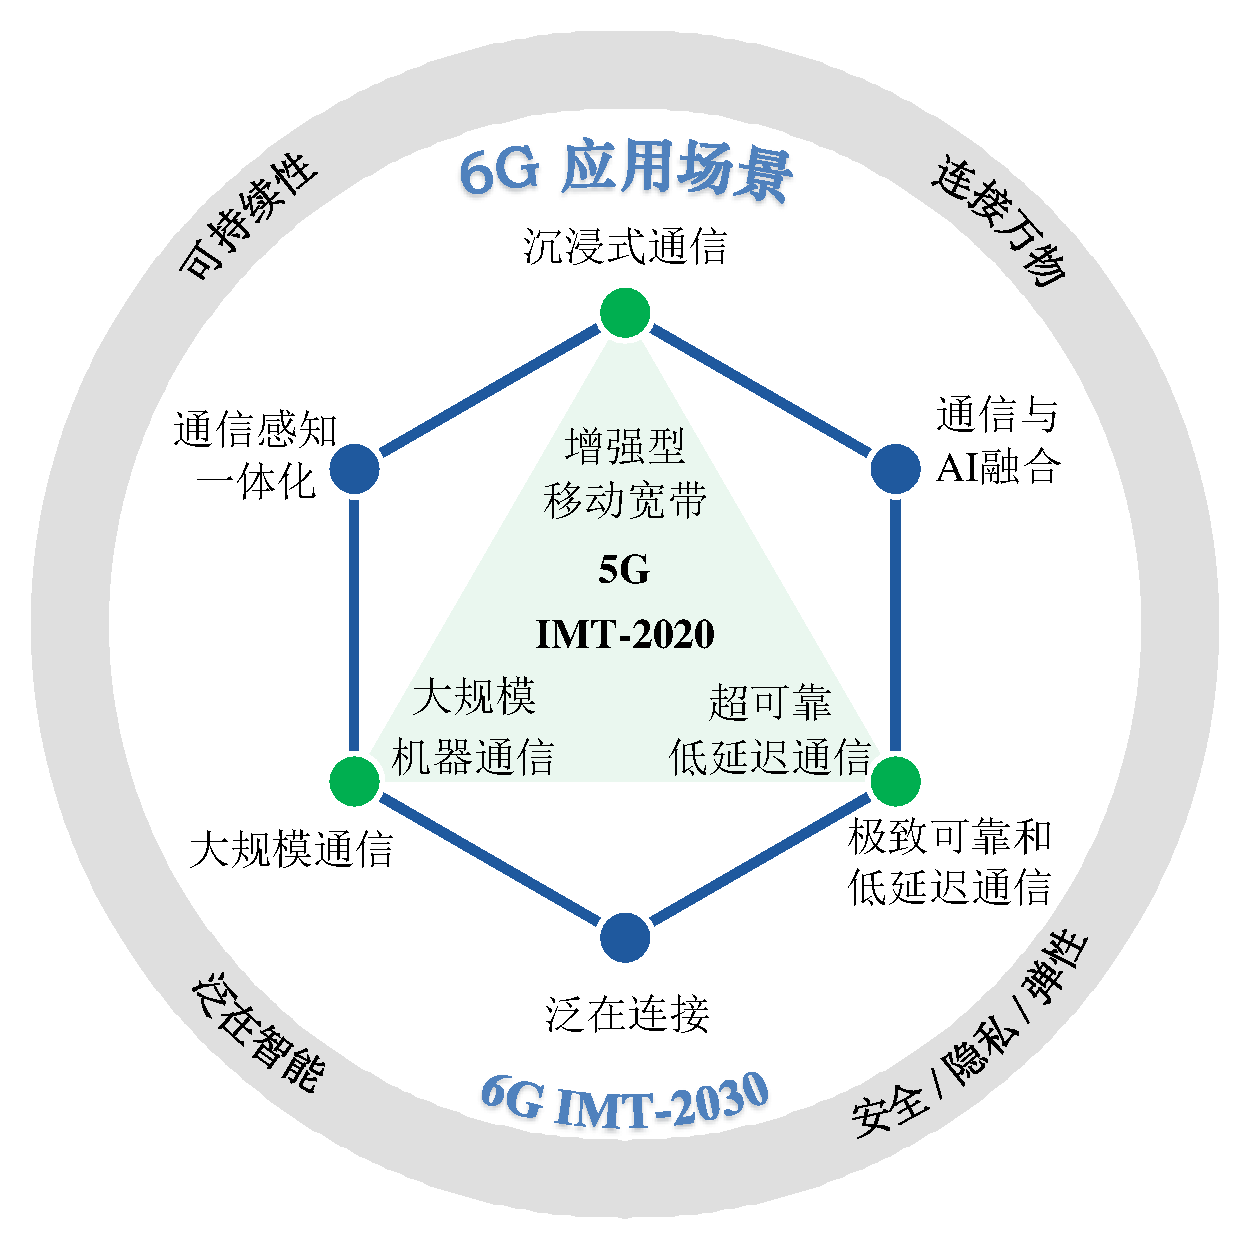
\includegraphics[width=\linewidth]{intro/intro_6G_usage_scenarios.pdf}
		\caption{6G典型应用场景}
		\label{fig:intro_6G_usage_scenarios}
	\end{subfigure}% % 这里的 % 很有必要，防止产生多余空格导致换行
	\hfill % 在两个子图之间自动填充间距
	% 第二张子图
	\begin{subfigure}[b]{0.46\linewidth}
		\centering
		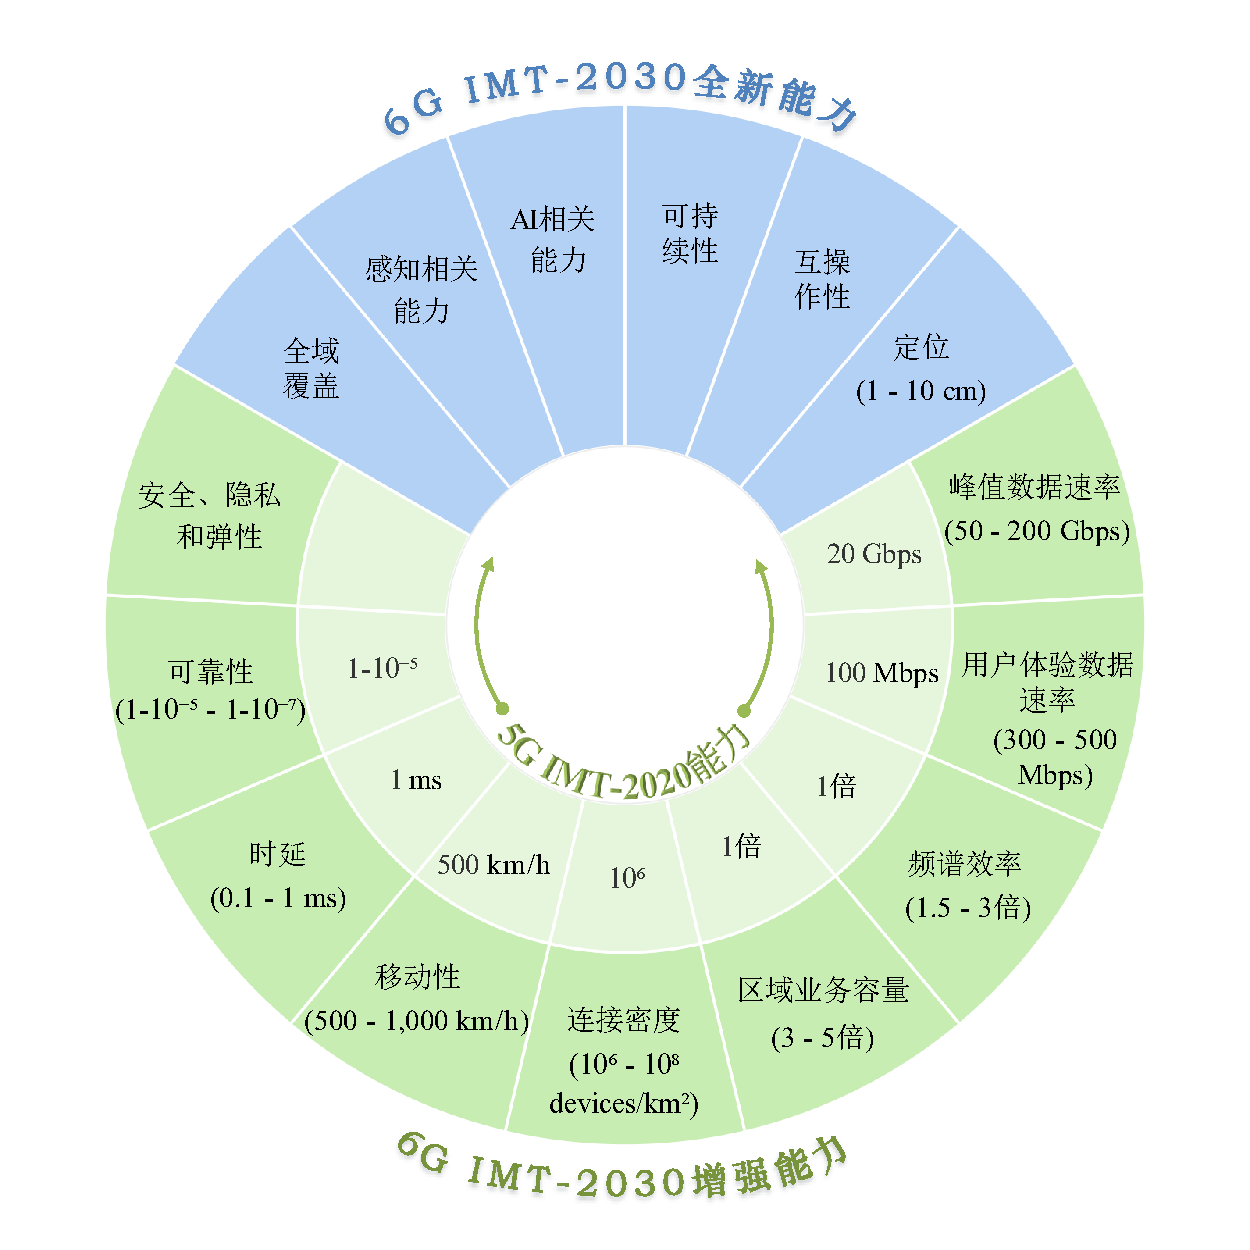
\includegraphics[width=\linewidth]{intro/intro_6G_performance.pdf}
		\caption{6G与5G性能指标对比}
		\label{fig:intro_6G_performance}
	\end{subfigure}
	\vspace{-0.5cm}
	\caption{IMT-2030中提出的6G愿景与性能指标\cite{ITU2023M2160}}
	\label{fig:intro_6G_imt}
\end{figure}

2023年11月，国际电信联盟（International Telecommunication Union, ITU）发布了6G建议书\cite{ITU2023M2160}，书中明确提出6G网络的六大典型应用场景，如图~\ref{fig:intro_6G_imt}(a)所示。其中包含对5G的原有场景提出了更高的要求，分别是：沉浸式通信、大规模通信和极致可靠和低延时通信，另外引入了通信感知一体化（Integrated Sensing and Communication, ISAC）、通信与人工智能（Artificial Intelligence, AI）融合和泛在连接三大全新应用范式。为了实现这些愿景，ITU为6G网络提出了15个具体的性能指标维度要求，如图~\ref{fig:intro_6G_imt}(b)所示。具体而言，九大增强型能力指标在5G原有能力上拓展，数据速率、频谱效率和能量效率均要求数倍于5G性能；六大全新能力涵盖全域覆盖、感知能力、定位能力、AI能力、可持续性和互操作性，要求6G网络向智能化、一体化发展。

然而，5G系统中广泛使用的技术已经不能很好地适应这些新需求。一方面，传统的mMIMO技术由有源相控阵实现，通过在基站侧和用户侧配置多根天线，可以带来信道容量的提升，且增益正比于天线数量\cite{asplund2020advanced,bjornson2016massive,yin2020addressing}。为实现6G中更高的频谱效率要求，所需的天线数量将剧烈增长，这不仅受到系统物理尺寸和复杂度的制约，大量的射频链路还会引起不可忽视的成本和功耗问题\cite{dohler2010cooperative}。另一方面，现有的蜂窝网络普遍受限于既定的物理传播环境，依靠更高的建站密度提升非视距（Non-Line-of-Sight, NLoS）覆盖，实现“全域覆盖”将进一步推高网络的建设和运营成本。在6G对高性能与低功耗双重要求的背景下，需要打破传统的通信架构，由“适应信道”的旧范式转变为“主动改变信道”的新设计范式，力求实现高效节能通信。

因此，如何构建智能电磁环境成为6G技术演进的重要突破方向。可重构天线系统（Reconfigurable Antenna System, RAS）这一新型体系结构，能够主动调控电磁波的传播行为，实现“重构信道”，已经成为6G物理层系统架构中的重要研究方向之一。广义而言，RAS是指一类能够在相位响应、幅度响应或空间分布等维度实现动态调控的天线阵列或电磁表面，其核心目标是在尽量降低硬件复杂度的前提下，实现对电磁波传播路径和特性的主动控制，有效解决传统mMIMO技术在成本、能效与部署方面面临的挑战。根据系统部署位置及重构方式的不同，现有RAS相关研究可大致划分为三类具有代表性的技术路径：第一类为部署于发射端，用以取代或简化有源相控阵的动态超表面天线（Dynamic Metasurface Antenna, DMA）\cite{smith2017analysis}；第二类为同样部署于发射端，但通过调整天线空间位置可实现大尺度信道重构的捏合天线系统（Pinching Antenna Systems, PASS）\cite{ding2025flexibleantenna}；第三类为部署在基站（Base Station, BS）与用户设备（User Equipment, UE）之间，用于构建视距链路（Line-of-Sight, LoS），改善覆盖条件的可重构智能表面（Reconfigurable Intelligent Surface, RIS）\cite{liu2021reconfigurable}。下文将对上述三类可重构天线技术的基本原理与典型特征进行简要介绍。

其中，动态超表面天线侧重于基站侧的体系结构革新，不同于传统相控阵高度依赖射频链路或移相器网络进行相位调节，DMA通过在波导或谐振腔表面集成大量包含正-本征-负（Positive-Intrinsic-Negative, PIN）二极管、变容二极管等可调谐元件的超材料单元，实现对电磁波幅度和相位的直接调控。借助对单元谐振状态的独立控制，DMA能够显著减少天线阵列中射频链路的数量，从而降低硬件复杂度和系统功耗，为超大规模天线阵列的工程实现提供了可行路径。然而，这种以波导馈电和单元辐射为特征的结构形式，也使DMA的信号传输过程不可避免地受到波导传播效应及单元耦合特性的共同影响，其可实现的波束增益及性能边界有别于传统相控阵。因此，有必要从理论层面对DMA的波束赋形机制及其性能极限进行系统分析。

在此基础上，捏合天线系统进一步从空间层面拓展了可重构自由度。捏合天线（Pinching Antenna, PA）又称夹子天线，介质波导上被夹子夹住的地方，介电常数会发生变化，电磁波便会辐射出来。利用这一性质，将DMA中波导上的超材料单元替换成这种可以沿着波导移动的“夹子”，使其具有位置可调的新自由度。该特性使捏合天线系统能够主动选择有利的空间位置，以规避深度衰落的区域并降低路径损耗，同时为高精度定位与感知提供更为丰富的空间信息。但实际部署中天线位置的移动往往伴随着馈电波导长度的改变，使信号在波导中传输和自由空间传播这两个过程存在紧密的耦合关系。上述因素使捏合天线的位置优化复杂化，需要针对性进行性能分析与算法设计。因此，有必要建立符合物理传播特性的PASS传输模型，定量刻画空间自由度引入所带来的性能增益，并进一步探索PA位置信息辅助下的通感一体化波束赋形机制。

与DMA和PASS侧重于发射机自身的重构不同，RIS将重构对象拓展至无线传播环境本身。RIS是一种由大量的亚波长人工结构单元组成的平面阵列，具备调控电磁波幅度、相位或极化的能力。与DMA类似，RIS单元通常由电阻、电容、电感和二极管等无源元件构成，调节加载在单元上的电压值，能产生不同的响应。于是，通过对各单元反射相位的协同调控，RIS能够重塑电磁波的传播路径，实现信号在空间中的定向反射与聚焦。由于RIS能够以极低的功耗人为构建绕过障碍物的视距链路，它很适合作为部署于基站与用户之间的辅助通信节点，在提升覆盖的同时降低系统能耗。然而，RIS作为独立于收发机之外的即插即用型系统，通常难以与基站或终端协同完成信道估计过程；同时，其自身缺乏独立的射频链路，难以直接感知获取信道状态信息（Channel State Information, CSI），使得依赖完备CSI的传统波束赋形与优化方法难以适用。因此，如何设计无需信道状态信息的低复杂度波束赋形算法，并在算法与工程实现之间建立可行的衔接路径，构建可实际部署的原型系统，是RIS技术走向商用的关键前提。

尽管DMA、PASS与RIS在具体实现形式和调控维度上各有侧重，但三者的核心目标一致，即通过引入新的信道调控自由度，实现对电磁传播环境的精细控制。无论是简化射频结构、重构天线空间位置，还是调控传播环境，其最终效果均体现为波束赋形能力的重塑及系统性能的提升。因此，围绕波束赋形机理、实际场景中的性能分析以及低复杂度算法实现开展研究，构成了可重构天线系统在6G物理层设计中的共同理论基础。下一节将分别综述三类可重构天线技术的代表性研究成果并总结目前面临的挑战。


\section{国内外研究现状与挑战}\label{sec:current_research_and_challenge}

\subsection{动态超表面天线研究现状与挑战}

如前文所述，动态超表面天线的核心是引入了包含可调谐元件的超材料单元。超材料这一概念在20世纪60年代由前苏联理论物理学家维克托·韦谢拉戈提出，他预言了磁导率和介电常数同为负值的左手材料的存在。他在研究中指出，当电磁波在这种介质中传播时，其电场矢量、磁场矢量与波矢量三者之间的方向关系，不再符合经典电磁学所描述的右手定则，而表现为左手关系\cite{veselago1968electrodynamics}。其传播相速度的方向与能量流动的方向恰好相反，将产生“负折射”的现象。这一现象为控制电磁波的传播开拓了新的可能性\cite{engheta2006metamaterials}。然而，受限于实验技术和制作工艺，这一构想被长期搁置，在当时并未引起足够的关注。

20世纪末，随着材料科学的不断进步，研究者们通过在材料上设计精细的微观结构，逐步制备出具备负磁导率和负介电常数的人工材料，并在此基础上开展对电磁波调控的研究。1996年，英国的J. B. Pendry教授提出了设计负介电常数结构的思路，利用周期性金属细线阵列结构，将金属的有效等离子体频率大幅降低至微波频段，实现了在该频段下具有等效负介电常数的人工超材料\cite{pendry1996extremely,pendry1998low}。随后，这一团队在1999年进一步提出了实现负磁导率超材料的结构方案：采用亚波长尺寸的金属开口谐振环组成周期性阵列，通过人为设计可使该结构表现出负磁导率特性\cite{pendry1999magnetism}。Pendry 教授主要贡献在于提出了较为完善的超材料设计理论，直至2001年，杜克大学的D. R. Smith教授团队首次采用印刷电路板（Printed Circuit Board, PCB）工艺成功制备出实物，并在实验中观测到了双负现象，验证了超材料相关理论的正确性\cite{smith2000composite,shelby2001experimental}。

相较于结构复杂、加工难度高的传统三维体态超材料，二维超表面以其低剖面、易集成的特点，成为一种新兴的超材料形态，能够有效简化制造工艺并降低集成复杂度\cite{chen2016review}。







\noindent\rule{\linewidth}{2pt}

随着制造工艺与电磁理论的不断演进，三维的体态超材料逐渐向低剖面、易集成的二维超表面形态过渡。正是在这种通过人工微结构重塑电磁波行为的长期积淀下，D. R. Smith 团队顺理成章地将超材料技术引入了微波天线的设计中，开创性地提出了一种颠覆传统射频架构的波导馈电动态超表面天线（Dynamic Metasurface Antenna, DMA）模型\cite{smith2017analysis}。



这种全新的架构将微带波导或二维谐振腔作为信号传输的骨架，在其表面密集嵌刻了大量亚波长尺寸的辐射缝隙。更为精妙的是，每个辐射单元内部均集成了如PIN二极管等有源可调器件。在发射状态下，基带信号仅需由极少量的射频链路注入波导。当导波在结构内部向前传播时，受数字指令控制的二极管会动态改变各个辐射单元的电磁谐振状态，使导波以漏波（Leaky-wave）的形式耦合至自由空间。这种设计直接在天线的物理辐射端完成了波束赋形的幅度与相位重构，彻底剥离了传统相控阵对庞大移相器网络和密集射频链路的依赖。凭借其低剖面、低功耗以及极简馈电的颠覆性优势，DMA迅速成为6G超大规模天线系统演进路径上极具潜力的研究焦点。



在向6G演进的进程中，天线阵列规模的持续扩张与硬件能耗之间的矛盾已成为无线通信物理层设计中难以回避的核心痛点。现有的全数字或混合预编码架构，本质上依赖于庞大的射频链路群与精密（且高功耗）的移相器网络来实现大规模MIMO的波束赋形。然而，当天线数量达到数百乃至上千级别时，这种“堆叠硬件”的传统相控阵设计思路在成本控制、馈电网络布线以及散热管理上均面临着难以逾越的物理瓶颈\cite{bjornson2017massive}。要从根本上打破这一僵局，就必须在天线的底层物理机制上寻求突破，而近年来超材料（Metamaterials）在电磁波调控领域的快速发展，恰好为重构天线阵列形态提供了全新的技术土壤\cite{cui2010metamaterials}。
通过将超材料的亚波长周期性结构与微波传输线相结合，杜克大学D. R. Smith团队首次提出了一种全新的天线架构——动态超表面天线（Dynamic Metasurface Antenna, DMA）\cite{smith2017analysis}。这种架构从根本上颠覆了传统天线的馈电与辐射机制。在具体实现上，DMA通常由一维微带波导或二维谐振腔构成主体，并在其表面密集排列大量亚波长尺寸的辐射单元。这里的关键在于，每个辐射单元不仅是物理意义上的“天线缝隙”，更是一个加载了PIN二极管或变容二极管的可调谐电磁谐振器\cite{shlezinger2019dynamic}。
从信号传输的视角来看，DMA的工作机理非常独特。在发射端，携带基带信息的电磁波只需由极少量的射频链路注入到微带波导的起始位置。当导波在波导内部向前传输时，它会依次经过表面的各个辐射单元，并通过电磁耦合以漏波（Leaky-wave）的形式向外辐射。由于表面每个单元的谐振状态均受其内部二极管偏置电压的独立控制，基站只需通过极低功耗的数字指令改变这些电压状态，就能直接在物理层面上对辐射出去的电磁波幅度与相位进行联合重构。这种将复杂的基带波束赋形操作下沉至天线物理辐射层的设计，不仅使系统摆脱了对密集射频链路的依赖，还在剖面尺寸和功耗上展现出传统相控阵难以企及的优势，为面向未来的超大规模智能天线设计开辟了一条极具工程潜力的技术路线。

如前文所述，为了满足6G网络对极高频谱效率与全域覆盖的严苛要求，基站端配置的天线阵列规模正向着超大阵列（Ultra-Massive MIMO）加速演进。然而，传统的全数字或混合相控阵天线架构通常需要为大量的天线振子配备独立的射频链路（RF Chains）与高精度的移相器网络。随着阵列规模的成倍扩张，庞大的射频硬件不仅导致系统成本与功耗呈指数级激增，其复杂的微带馈电布线也在高频段（如毫米波系统）面临着严重的物理空间与电磁互耦瓶颈\cite{bjornson2017massive}。为了打破这一“功耗-成本-尺寸”的工程瓶颈，研究人员开始寻求天线底层物理架构的根本性变革，而超材料（Metamaterials）技术的突破恰好为此提供了契机。

超材料是由亚波长尺度的人工微结构按特定空间排列方式构成的新型电磁材料。它突破了自然材料的电磁属性限制，能够实现负折射率、完美吸收以及异常反射等奇异的电磁调控现象\cite{cui2010metamaterials}。随着该技术的不断成熟，杜克大学（Duke University）的 D. R. Smith 团队将其与传统导波结构相结合，于近年来开创性地提出了一种基于波导馈电的动态超表面天线（Dynamic Metasurface Antenna, DMA）架构\cite{smith2017analysis}。

与传统相控阵复杂的树状馈电网络或自由空间馈电不同，DMA 巧妙地在一维微带波导或二维谐振腔体的表面，密集刻蚀了大量亚波长尺寸的辐射单元（Metamaterial Elements）以形成物理阵列。每一个辐射单元本质上是一个可调谐的电磁谐振器，其内部集成了正-本征-负（PIN）二极管或变容二极管（Varactor Diodes）等有源固态半导体器件\cite{shlezinger2019dynamic}。在DMA的工作过程中，基带信号仅需通过极少数的射频链路馈入波导的起始端。当电磁波在波导内部向前传播时，会与表面的超材料辐射单元发生电磁耦合，从而形成向自由空间辐射的漏波（Leaky-wave）。基站控制器通过外部指令动态调节各单元内二极管的偏置电压，即可独立改变每个超材料单元的谐振频率，进而在天线的物理辐射层面实现对电磁波幅度与相位的直接重构。这种创新架构将波束赋形操作从高功耗的数字基带转移到了天线物理层，极大地压缩了所需的射频链路数量，凭借其低剖面、低功耗的显著优势，成为了学术界公认的下一代大规模天线演进方向之一。



超材料（Metamaterials）是由亚波长尺度的人工微结构按特定空间排列方式构成的新型电磁材料。它突破了自然材料的电磁属性限制，能够实现负折射率、完美吸收以及异常反射等奇异的电磁现象\cite{cui2010metamaterials}。随着超材料技术的不断成熟，其在天线设计领域的应用逐渐成为学术界与工业界的研究热点。传统的大规模MIMO和毫米波通信系统高度依赖于全数字或混合相控阵架构，这类架构通常需要为每根天线或子阵列配备独立的射频链路（RF Chains）与高精度移相器。随着天线规模的急剧增加，系统的硬件成本、馈电网络布线难度以及射频功耗均呈现出难以接受的线性甚至指数级增长\cite{bjornson2017massive}，成为了制约6G大阵列系统走向实用化的核心瓶颈。

\noindent\rule{\linewidth}{2pt}

超材料（Metamaterial）是一类通过人工设计的周期性或非周期性微结构单元构成的复合材料，其电磁特性主要取决于单元结构的几何形状与空间排列方式，而非材料的本征属性。这一独特特性使得超材料能够展现出天然材料所不具备的电磁响应行为，例如负折射率、完美吸收、电磁波极化调控等奇异现象。自21世纪初Pendry等人关于完美透镜的开创性工作以来，超材料在电磁波调控领域的研究取得了蓬勃发展，并逐渐从基础物理研究走向工程应用。在天线设计领域，超材料的应用为突破传统天线性能瓶颈提供了全新思路。传统天线设计往往受限于材料的固有属性和几何尺寸，而超材料天线通过精心设计单元结构，可以实现对电磁波传播方向、极化状态、频率响应等特性的灵活调控，从而显著提升天线的增益、带宽、扫描范围等关键性能指标。

在超材料天线的发展历程中，动态超表面天线（Dynamic Metasurface Antenna, DMA）的提出标志着一个重要里程碑。2017年，Smith团队在文献中首次系统地提出了波导馈电DMA的概念与理论模型。与传统相控阵天线依赖大量射频链路和移相器实现波束扫描不同，DMA采用了一种创新性的架构设计：将亚波长尺度的超材料辐射单元嵌入波导或腔体结构中，通过外部控制信号调节每个单元的电磁响应特性，从而实现对辐射波前的程序化调控。在Smith团队提出的波导馈电DMA模型中，每条波导上均匀分布着若干超材料辐射单元，输入信号经由波导传输并逐级馈电至各个单元，最终由单元向自由空间辐射。这一架构的核心优势在于，它仅需要与波导数量相等的射频链路，而非与辐射单元数量相等的射频链路，从而大幅降低了系统的硬件复杂度和功耗成本。

从物理建模角度，Smith团队的研究揭示了DMA辐射单元的频率响应呈现出典型的洛伦兹谐振特性。具体而言，每个超材料单元可视为一个可调谐的谐振电路，其频率响应可通过调节单元的谐振频率进行外部控制。对于窄带通信系统，单元的响应可以简化为洛伦兹约束形式$q = (j + e^{j\phi})/2$，其中$\phi$为可配置的相位偏移参数。这一数学形式揭示了DMA设计中面临的一个关键挑战：单元的幅度响应与相位响应存在固有的耦合关系，而非传统相控阵中相互独立的幅度和相位控制。这种耦合特性使得DMA的波束赋形优化问题具有独特的数学结构，既不同于传统的数字预编码问题，也不同于基于单位模约束的移相器优化问题。Smith团队的工作不仅建立了DMA的理论分析框架，还深入探讨了互耦效应、波导衰减、单元间距等实际因素对系统性能的影响，为后续DMA在无线通信领域的应用研究奠定了坚实基础。



\noindent\rule{\linewidth}{2pt}



为了突破传统相控阵天线的物理与功耗瓶颈，杜克大学（Duke University）的 D. R. Smith 团队于近年来开创性地提出了一种基于波导馈电的动态超表面天线（Dynamic Metasurface Antenna, DMA）架构\cite{smith2017analysis}。与传统相控阵复杂的微带馈电网络或自由空间馈电不同，DMA 在一维微带波导或二维谐振腔体的表面密集刻蚀大量亚波长尺寸的辐射单元（Metamaterial Elements）以形成物理阵列。每一个辐射单元本质上是一个可调谐的电磁谐振器，其内部集成了正-本征-负（PIN）二极管或变容二极管（Varactor Diodes）等有源固态半导体器件\cite{shlezinger2019dynamic}。

在DMA的工作过程中，基带信号仅需通过极少数的射频链路馈入波导的起始端。当电磁波在波导内部向前传播时，会与表面的超材料辐射单元发生电磁耦合，从而形成向自由空间辐射的漏波（Leaky-wave）。基站控制器通过外部的现场可编程逻辑门阵列（FPGA）或微控制器发出数字指令，动态调节各单元内二极管的偏置电压，即可独立改变每个超材料单元的谐振频率，进而实现对辐射电磁波幅度与相位的直接重构。这种创新的物理架构巧妙地将波束赋形操作从高功耗的基带数字预编码或射频移相器网络，转移到了天线阵列的物理辐射层面。它不仅极大地压缩了多天线系统所需的射频链路数量，还凭借其低剖面、低成本、低功耗的显著优势，为6G超大规模天线阵列的工程部署提供了一种极具潜力的革命性替代方案。

\noindent\rule{\linewidth}{2pt}

\begin{figure}[!htbp]
	\centering
	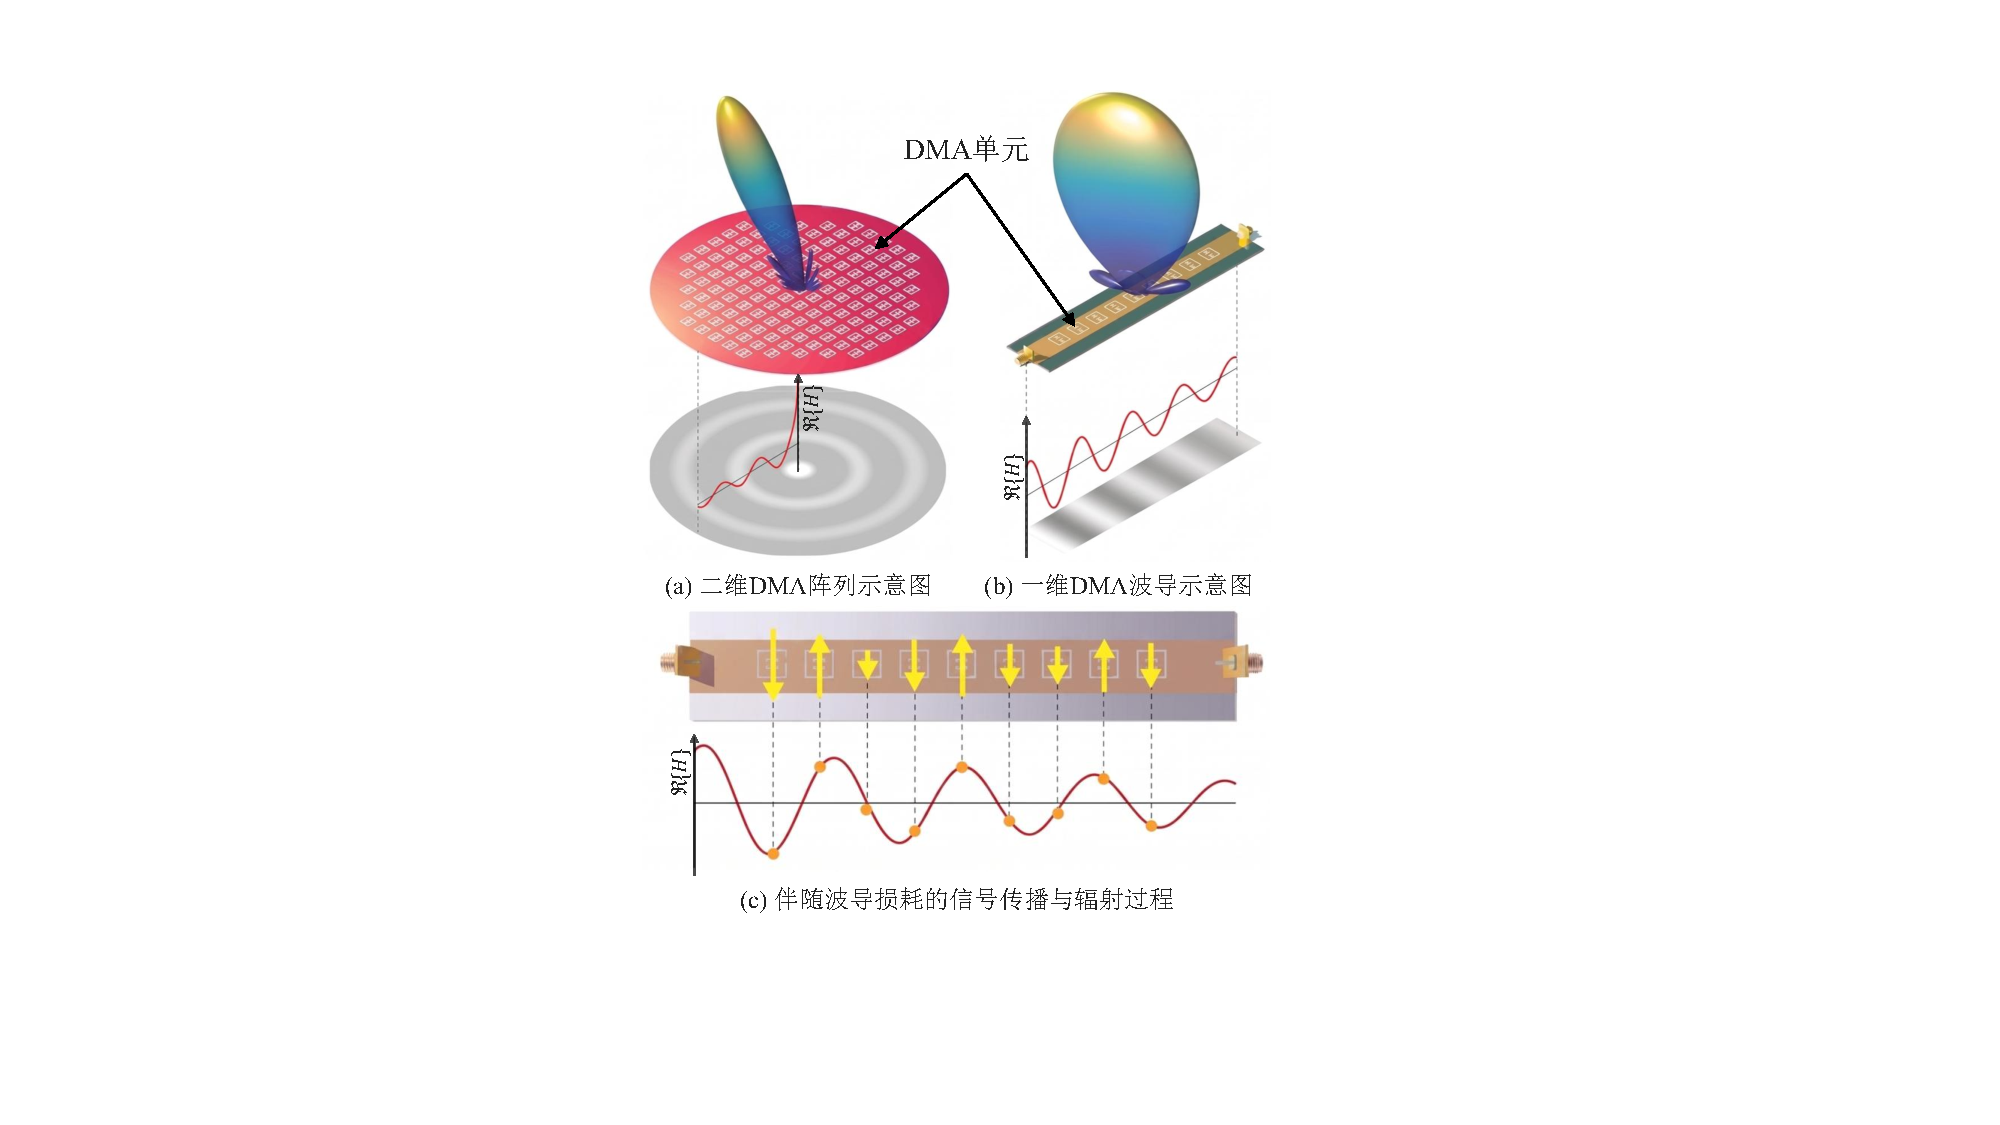
\includegraphics[width=0.5\linewidth]{intro/intro_DMA_waveguide_loss.pdf}
	\caption{动态超表面天线结构及工作原理示意图\cite{yoo2019enhancing}}
	\label{fig:intro_DMA_waveguide_loss}
\end{figure}



SIW

介绍第一次提出


介绍洛伦兹约束

从极化率的角度详细分析为什么会相依能力不足


介绍波束赋形算法

介绍性能分析现状

介绍挑战


这一部分需要展示对DMA底层机理的深刻理解，并精准地指出当前理论研究与工程实现之间的脱节，从而为你后续提出“离散算法”和“量化分析”做铺垫。

以下是为你撰写的 **1.2.1 动态超表面天线 (DMA) 研究现状**，语言风格保持学术严谨，你可以根据实际引用的文献编号进行调整。

---

 1.2.1 动态超表面天线 (DMA) 研究现状

作为一种极具潜力的新型收发机架构，动态超表面天线（DMA）通过在波导或空腔结构上集成大量可调超材料单元，实现了对电磁波辐射特性的动态调控。与传统相控阵天线依赖移相器和独立射频链路不同，DMA利用超表面的物理特性进行信号处理，极大地简化了硬件架构。

**（1）DMA架构与洛伦兹谐振模型**
DMA的基本概念最早由杜克大学的D. R. Smith教授团队系统性提出[1]。其典型架构通常由微带线或波导作为馈电结构，表面周期性或准周期性地排列着亚波长超材料谐振单元。当导波在馈电结构中传输时，通过外部控制信号（如直流偏置电压）改变加载在单元上的电子元件（如变容二极管或PIN二极管）的状态，从而调节每个单元的辐射振幅和相位，最终在自由空间合成所需的波束方向图。

在理论建模方面，Smith等人提出了基于**洛伦兹（Lorentzian）谐振**的极化率模型来描述DMA单元的电磁响应[2]。在该模型中，第  个超材料单元的磁极化率  通常表示为：



其中， 为工作频率， 为单元的谐振频率， 为振荡强度， 为阻尼系数。通过调节电路参数改变谐振频率  或阻尼 ，即可改变单元对导波的耦合强度和辐射相位。这一模型揭示了DMA的一个关键物理特性：**幅度与相位是强耦合的**，即在改变相位的过程中，单元的辐射幅度也会随之遵循洛伦兹曲线发生非线性变化，这与传统相控阵中幅度相位独立调控的机制截然不同。

**（2）基于连续相位假设的波束赋形算法研究**
基于上述架构，早期的DMA波束赋形研究主要聚焦于全息波束赋形理论。其核心思想是将所需的波束方向图视为“目标物波”，将波导内的传输场视为“参考波”，通过优化超表面单元的阻抗分布来重建目标波前。为了简化优化问题，现有文献多采用**松弛（Relaxation）策略**，即假设超材料单元的谐振频率或相位响应可以在一定范围内**连续变化**。
在此假设下，研究者们将DMA的波束赋形建模为连续域上的数学优化问题，并利用最小二乘法（Least Squares）、梯度下降法或基于格林函数的迭代算法求解最优的单元配置权重[3-4]。这些基于连续性假设的算法在理论仿真中展示了DMA在多波束生成、干扰抑制及高维MIMO传输方面的巨大潜力。

**（3）现有研究的局限与挑战（Gap 1）**
尽管关于DMA的理论研究已取得显著进展，但将理论转化为实际工程应用仍面临严峻挑战，主要体现在以下两个方面：

首先，**理想连续相位假设与实际离散硬件约束存在鸿沟**。在工程实现中，为了降低控制电路的复杂度和成本，DMA单元通常采用1-bit（开/关）或低比特（如2-bit）的数字控制方案，即单元的相位响应只能取有限个离散值。现有的基于连续相位的算法直接应用于离散系统时，需要进行强制量化（Rounding），这将破坏波束赋形的相干性，导致严重的天线增益损失和旁瓣抬升。

其次，**缺乏针对离散与耦合约束的高效算法**。由于DMA单元遵循洛伦兹谐振模型，其**幅度和相位存在固有的非线性耦合**，且离散化后的波束赋形问题本质上是一个非凸的整数规划问题（Integer Programming）。现有的穷举搜索法随单元数量呈指数级复杂度，难以应用于大规模阵列；而传统的松弛算法在处理强耦合的离散约束时往往陷入局部最优。因此，**如何在考虑洛伦兹耦合约束和离散相位约束的前提下，设计低复杂度的波束赋形算法，并从理论上量化分析离散化带来的性能损失，是DMA技术走向实用化亟待解决的关键问题**。

---

 **参考文献标注建议：**

* [1] Sleasman T, Imani M F, Gollub J N, et al. Dynamic metasurface antennas as a new paradigm for radio detection and ranging[J]. Applied Physics Letters, 2015. (Smith团队的基础性论文)
* [2] Pulido-Mancera L, Sleasman T, Smith D R, et al. Analytical modeling of dynamic metasurface antennas[J]. IEEE Transactions on Antennas and Propagation, 2021. (洛伦兹模型的详细分析)
* [3] [插入你查阅的关于DMA连续相位优化的相关文献]
* [4] [插入你查阅的关于全息波束赋形算法的相关文献]

 **写作提示：**

这段文字明确了Gap 1：**“连续假设 vs. 离散现实”** 以及 **“幅相独立 vs. 洛伦兹耦合”**。这不仅指出了前人的不足，更直接为你第二章（性能极限分析）和第三章（离散算法设计）提供了最为坚实的立论依据。

\subsection{捏合天线系统研究现状}

介绍第一次提出NTT DOCOMO

介绍性能分析，介绍波束赋形，介绍定位，介绍通感或者感知。

介绍挑战






\begin{figure}[!htbp]
	\centering
	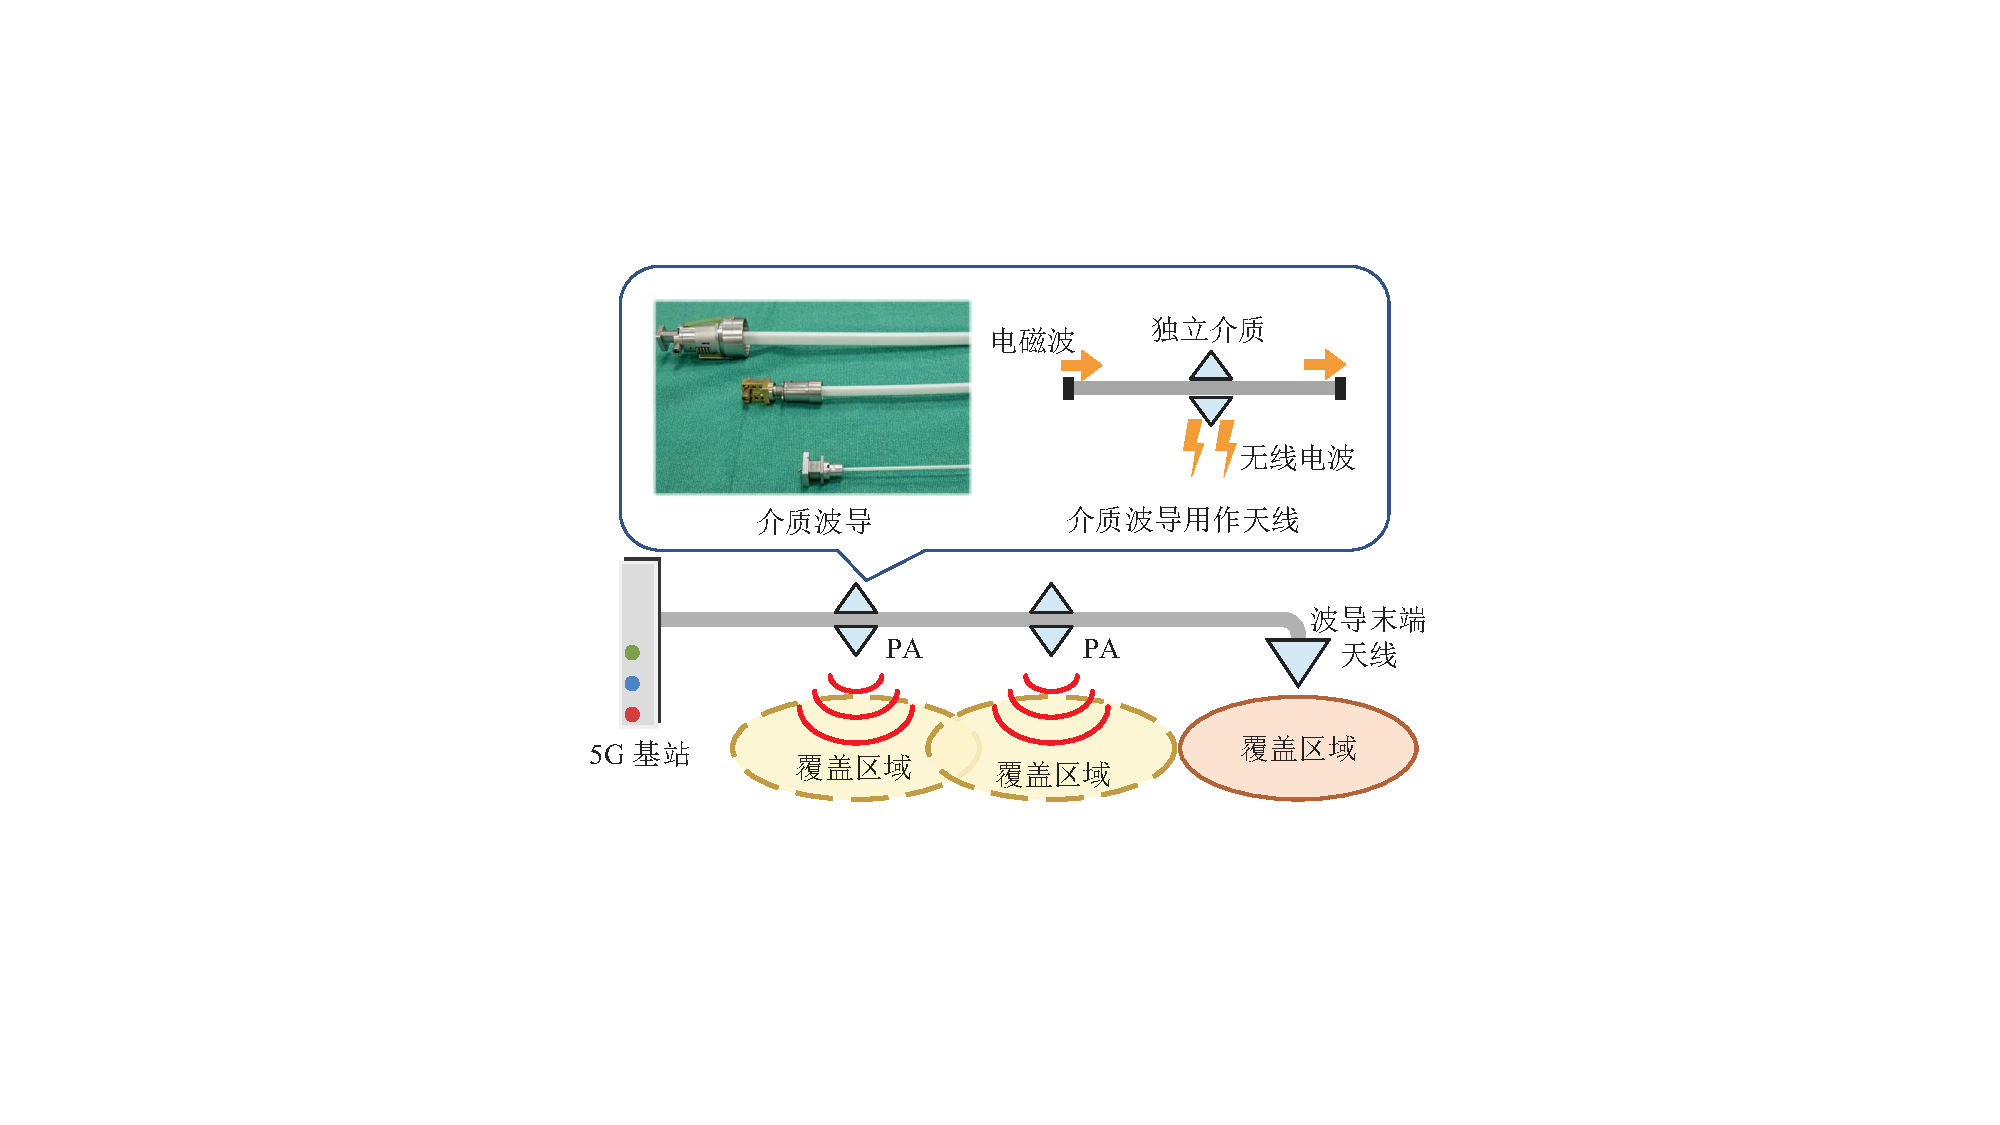
\includegraphics[width=0.6\linewidth]{intro/intro_PASS.pdf}
	\caption{使用捏合天线部署通信区域\cite{fukuda2022pinching}}
	\label{fig:intro_PASS}
\end{figure}


\begin{figure}[!htbp]
	\centering
	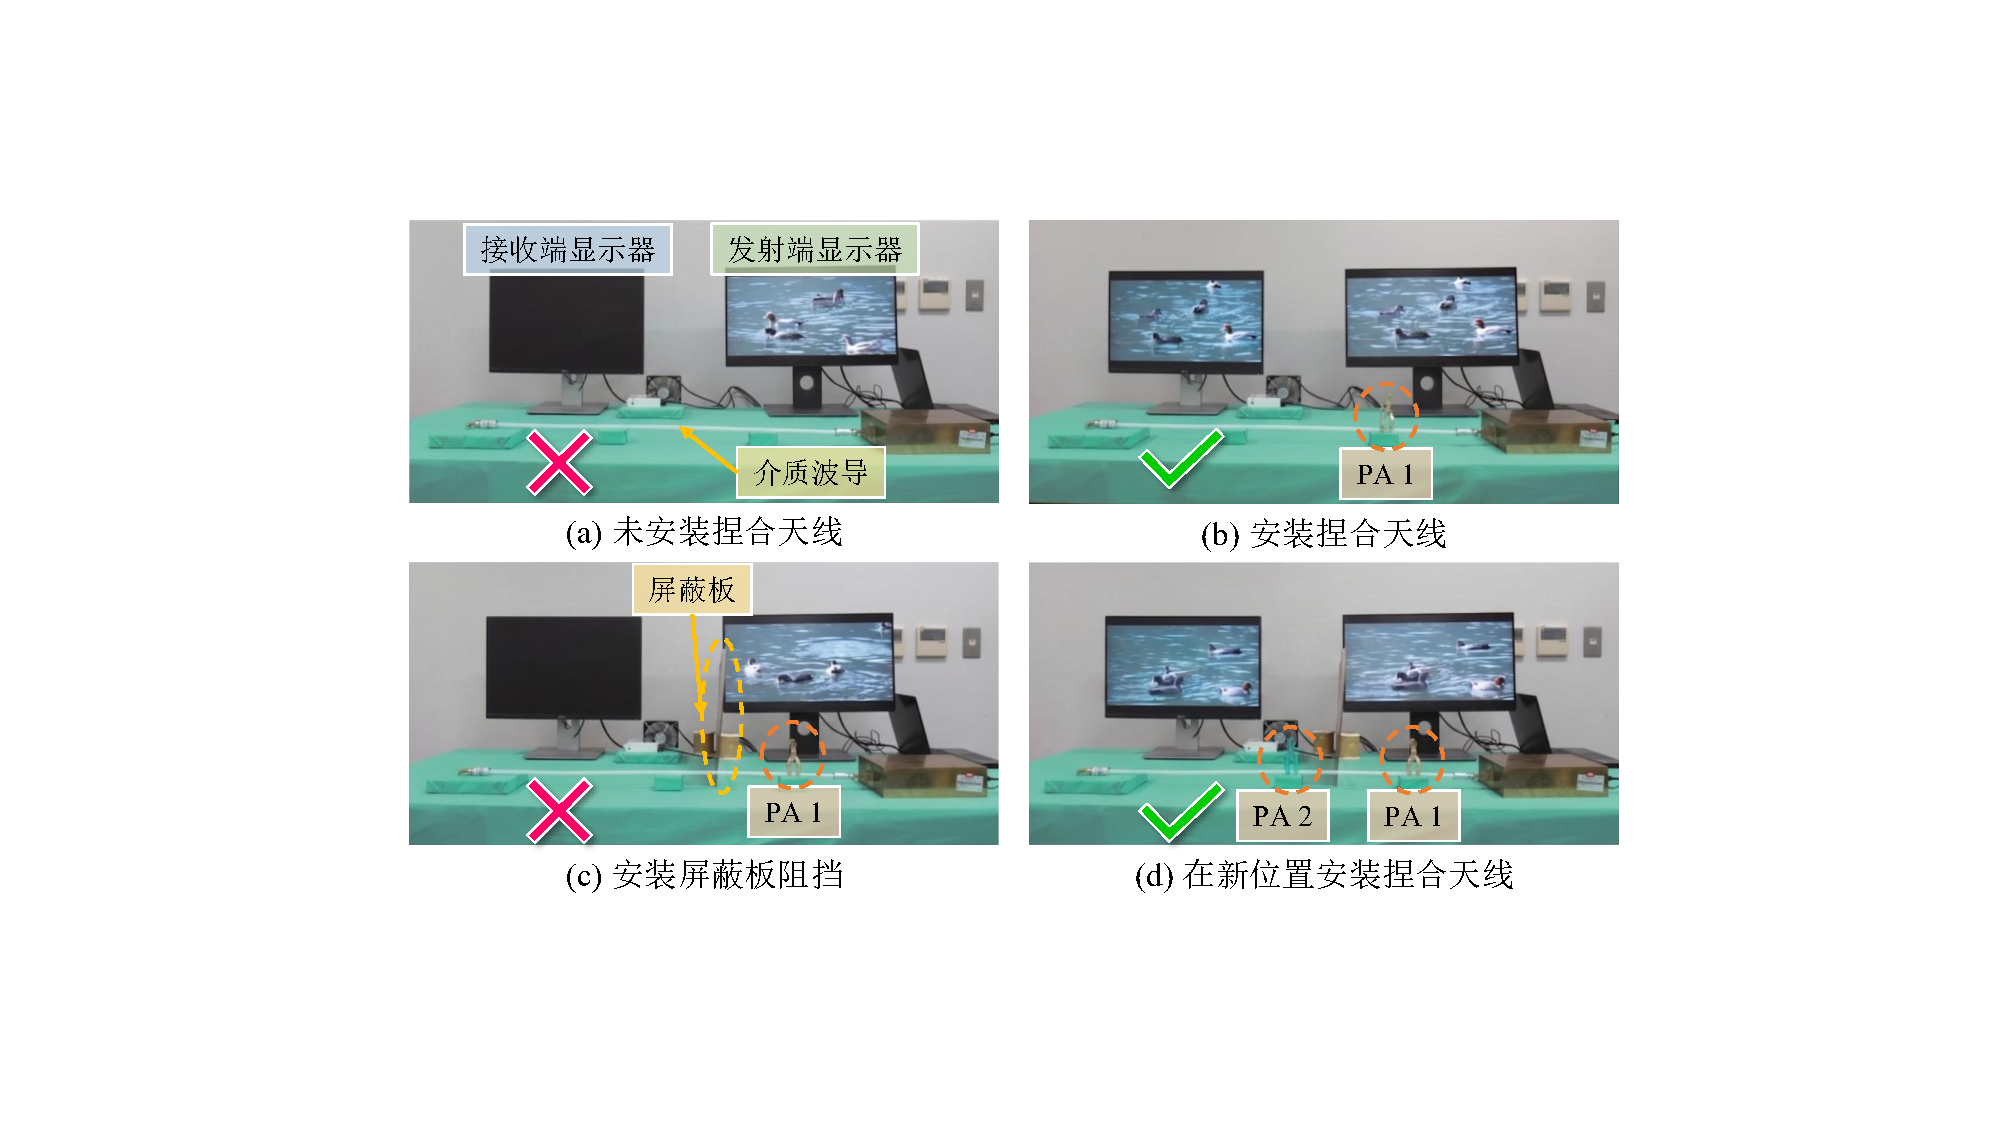
\includegraphics[width=0.7\linewidth]{intro/intro_PASS_demo.pdf}
	\caption{通过捏合天线进行视频传输实验\cite{fukuda2022pinching}}
	\label{fig:intro_PASS_demo}
\end{figure}

\subsection{可重构智能表面研究现状}

介绍基本概念第一次提出、崔铁军和RFocus

介绍波束赋形算法

介绍系统研制

介绍不足

\subsection{现有研究中存在的不足}

DMA的理论不完善

从体系结构角度看，DMA通过在发射端引入电磁响应可重构的超材料单元，显著降低了射频链路数量，为大规模阵列的低功耗实现提供了新的硬件基础。然而，这种结构性简化也使得波束赋形过程受到波导传播效应与单元耦合特性的联合约束，其可实现的波束空间及性能边界有别于传统相控阵，亟需从理论层面对其波束赋形机理与性能极限进行系统分析。

因此，可重构天线系统的性能分析与波束赋形算法设计仍然有许多尚未解决的问题

\section{研究内容与章节安排}\label{sec:content_and_arrangement}

\subsection{论文主要研究内容}\label{sec:content}

本文主要研究xxx

\subsection{论文章节安排}\label{sec:arrangement}

全文共分为7章。主要内容如下：

第1章 绪论：简要介绍论文的研究背景、国内外研究现状、存在的问题，给出全文的主要研究内容。为了让读者更容易理解全文，建议用一个文档结构图给出各章节逻辑关系。

第2章 样式使用说明：一般应介绍该章的主要内容，说明这一章做什么。

第3章 实验研究类论文：……

第4章 理论或算法类论文的结构：……

第5章 总结与展望：给出全文的主要内容及结论，总结本文的创新点，并对未来的工作进行展望。





 % 绪论
\chapter{连续相移DMA波束赋形性能分析与相位对齐算法}\label{ch:cdma}

\section{引言}

\textcolor{red}{之后再写}

\section{系统模型}\label{sec:cdma_system_model}

本章考虑基于DMA架构的下行链路通信系统，其中基站采用DMA作为发射阵列，为单天线用户提供通信服务。如图~\ref{fig:cdma_system}所示，输入信号先经过数字基带预编码处理，然后由射频链路馈入波导起始位置，经波导传输后由单元辐射。该DMA阵列包含包含$N_d$条平行的波导，每条波导上分布着$N_e$个亚波长间隔的超材料辐射单元，则单元总数量为$N \triangleq N_d \times N_e$。
每个辐射元件都被视为一个共振电路，令$q_{i,l}$表示第$i$条波导上第$l$个辐射单元的频率响应，其洛伦兹形式描述如下\cite{smith2017analysis}：
\begin{equation}\label{eq:cdma_qilf}
	q_{i,l}(f) = \frac{-\Omega f^{2}}{f^{2} - \hat f_{i,l}^{2} + j \Gamma f},
\end{equation}
其中$\Omega \in \mathbb R$是振荡器强度，$\hat f_{i,l}$是该单元的共振频率，$\Gamma$是阻尼因子。通过外部控制可以调节单元的共振频率，从而调控响应的幅度和相位。对于窄带系统，通常认为元件具有平坦的频率响应\cite{wang2021dynamic}。因此，每个DMA元素的响应呈现如下形式：
\begin{equation}\label{eq:cdma_qil}
	q_{i,l} =\frac{j+e^{j \phi_{i,l}}}{2}, \quad \phi_{i,l} \in [0, 2\pi),
\end{equation}
其中$\phi_{i,l}$是每个元素的可配置连续相位偏移。

\begin{figure}[!htbp]
	\centering
	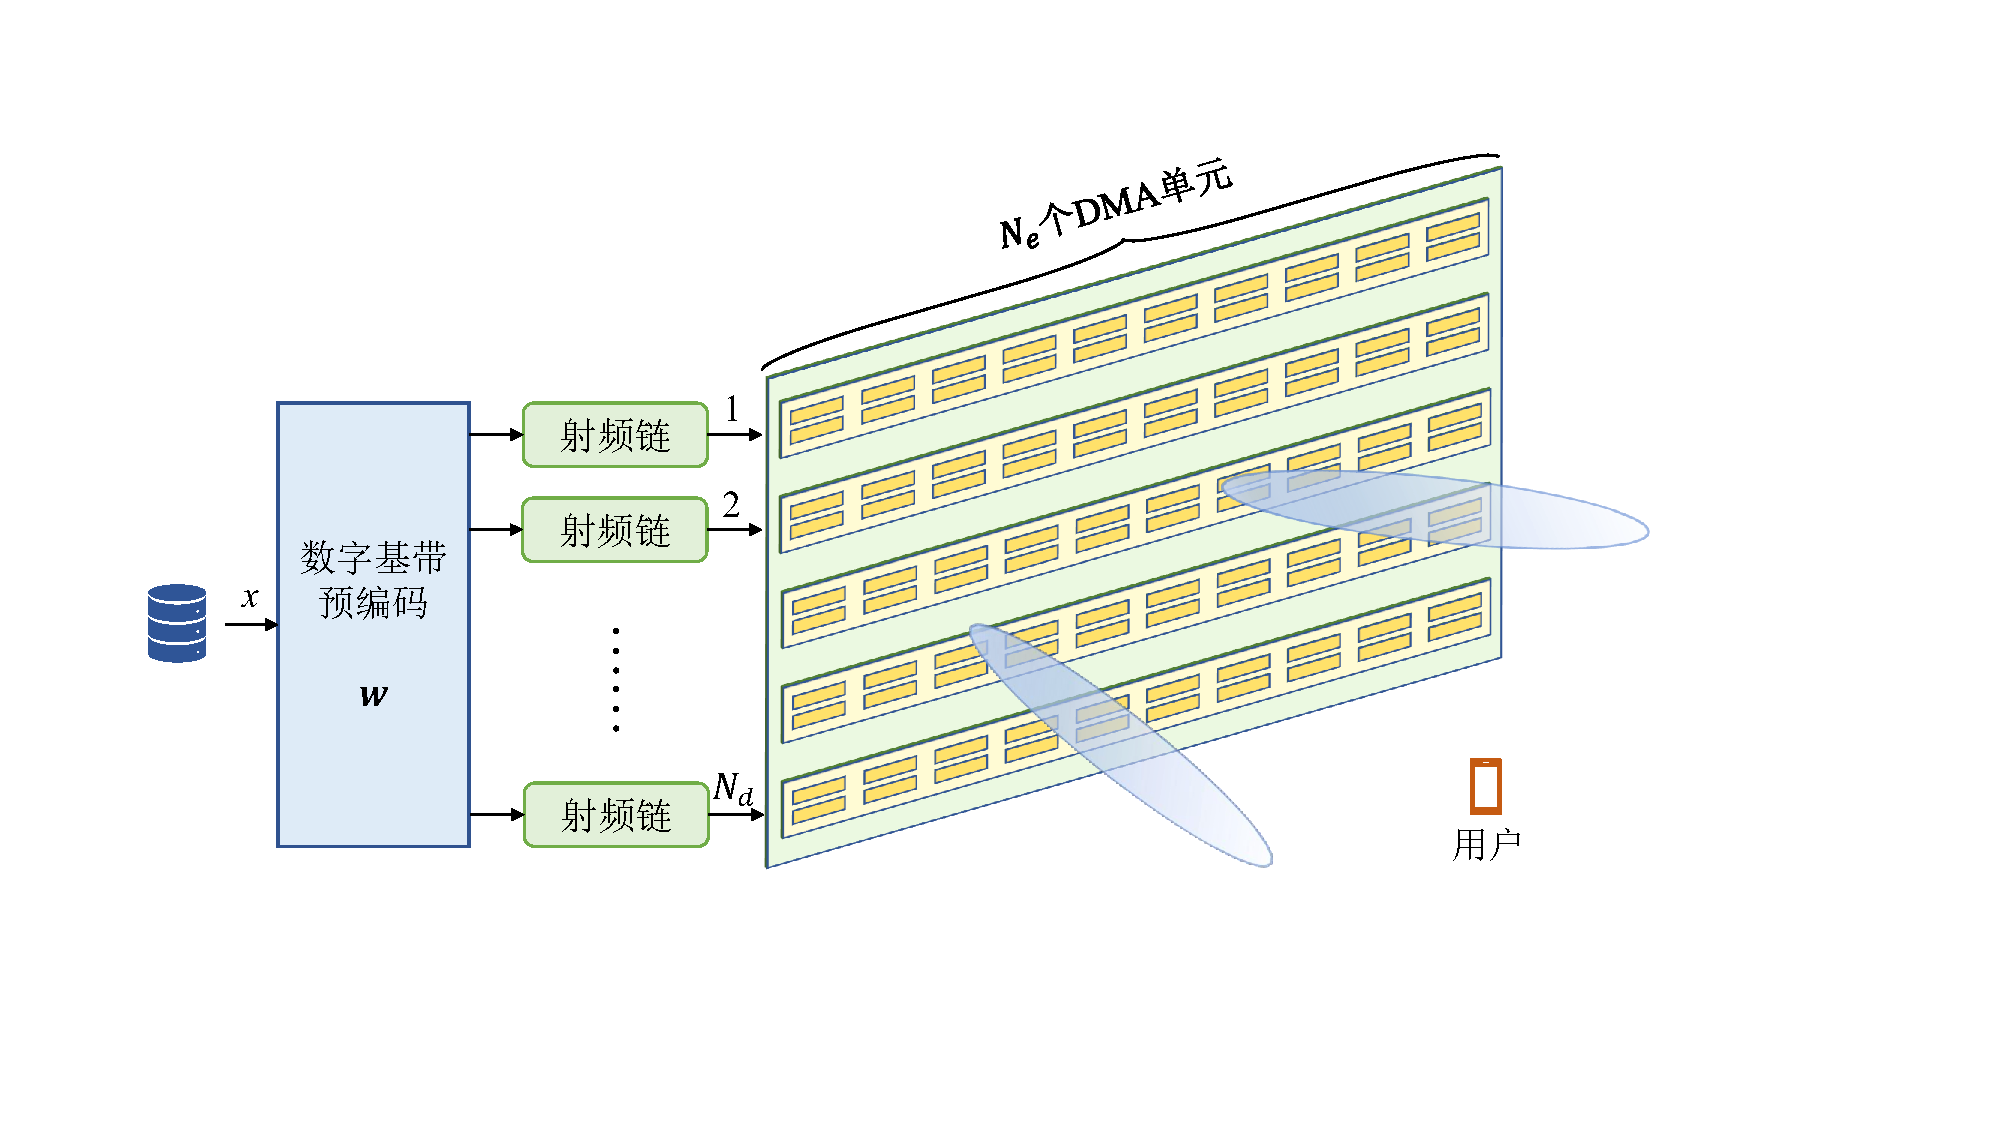
\includegraphics[width=0.8\linewidth]{cdma/cdma_system.pdf}
	\caption{动态超表面天线通信系统示意图}
	\label{fig:cdma_system}
\end{figure}

信号在波导内传输会经历传播时延和衰减，这个过程可以描述为：
\begin{equation}\label{eq:cdma_hil}
	h_{i,l} = \frac{1}{\sqrt{N_e}}e^{-\upsilon_{i,l}(\alpha + j\beta)},\quad \forall i,l,
\end{equation}
其中$\alpha$、$\beta$和$\upsilon_{i,l}$分别代表波导的衰减系数、波数以及第$l$个单元在第$i$个波导中的位置。通常，对于均匀的DMA阵列，$\upsilon_{i,l} = D(l-1)$，其中$D$表示单元之间的间距。归一化系数$1/\sqrt{N_e}$的引入确保了总功率是受到约束的。这样设定是因为随着单元数量的增加，每个单元可获取的功率会减少，为简化分析，假设波导上的单元都会因为其他单元的辐射而经历相同的整体衰减过程。

设$\bm{v} = [v_1, v_2, \cdots, v_{N_d}]^\mathrm{T} \in \mathbb{C}^{N_d \times 1}$表示基带输入到所有波导的向量。于是，DMA阵列辐射出的信号$\bm s \in \mathbb{C}^{N \times 1}$可以写为：
\begin{equation}\label{eq:cdma_s}
	\bm s=\bm{H Q v},
\end{equation}
其中$\bm H \in \mathbb{C}^{N \times N}$是描述所有波导信号传播效应的对角矩阵，由下式给出：
\begin{equation}\label{eq:cdma_H}
	\bm{H} = \operatorname{diag}\left( h_{1,1}, \cdots, h_{1,N_e}, h_{2,1}, \cdots, h_{2,N_e}, \cdots, h_{N_d,1}, \cdots, h_{N_d,N_e} \right).
\end{equation}
矩阵$\bm{Q}$是一个块对角矩阵，表示DMA单元的可配置权重。其形式如下：
\begin{equation}\label{eq:cdma_Q}
	\bm{Q} = 
	\begin{bmatrix}
		\bm{q}_1 & \bm{0} & \cdots & \bm{0} \\
		\bm{0} & \bm{q}_2 & \cdots & \bm{0} \\
		\vdots & \vdots & \ddots & \vdots \\
		\bm{0} & \bm{0} & \cdots & \bm{q}_{N_d}
	\end{bmatrix}
	\in \mathbb{C}^{N \times N_d},
\end{equation}
其中每个子块$\bm{q}_i \in \mathbb{C}^{N_e \times 1}$对应第$i$个波导上所有单元的权重：
\begin{equation}
	\bm{q}_i = 
	\begin{bmatrix}
		q_{i,1} \\
		q_{i,2} \\
		\vdots \\
		q_{i,N_e}
	\end{bmatrix},
	\quad i = 1,2,\ldots,N_d.
\end{equation}

需要指出的是，$\bm H$的对角线假设忽略了超表面单元之间的相互耦合。虽然互耦会影响模型的精度并降低系统性能，但是，当波导与超表面单元导波模式弱耦合时，通常这样简化\cite{smith2017analysis}。为了进一步减小互耦，可以在设计DMA阵列的时候采取一些常用的方法，例如将辐射元件从波导中心向边缘移动，减少相邻元件之间的共同场区域，在此基础上，可以让辐射单元在波导两侧交替排列，进一步增大单元之间的间距。在本章中，假设每个波导内的元件间距不小于半个波长，这有助于确保元件不会干扰波导模式，并且元件之间的相互作用可以忽略不计。

基站通过发送功率为$P_t$的单位符号$x$来为用户提供服务，并采用预编码向量$\bm w \in \mathbb{C}^{N_d \times 1}$进行预编码。因此，输入至DMA的发射信号可表示为$\bm v = \bm w x$。根据式~\eqref{eq:cdma_s}，用户端接收信号$y$可表示为：
\begin{equation}
	y=\sqrt{P_{t}}\bm{g}^\mathrm{T} \bm{HQw} x + \eta,
\end{equation}
其中，$\bm g =[g_{1,1}, \cdots, g_{1,N_e}, \cdots, g_{N_d,1}, \cdots, g_{N_d,N_e}]^\mathrm{T} \in \mathbb{C}^{N \times 1}$表示基站与用户之间的信道向量，在本章中，不失一般性，假设DMA阵列和用户之间为瑞利信道，即：$\bm g \sim \mathcal{CN}(\bm 0_{N\times1}, \sigma_g^2 \bm I_N)$，$\eta \sim \mathcal{CN}(0, \sigma^2)$为用户处的加性白高斯噪声（Additive White Gaussian Noise，AWGN）。

\section{DMA最优相位配置方法与性能分析}\label{sec:cdma_opt}

\subsection{波束赋形问题建模}

对于给定系统，在用户处的信噪比定义为：
\begin{equation}\label{eq:cdma_SNR}
	\mathrm{SNR}=\frac{P_{r}}{\sigma^2}
	=\frac{P_{t} \left| \bm{g}^\mathrm{T} \bm{HQw} \right|^2} {\sigma^2},
\end{equation}
其中$P_{r}$为用户的接收功率。为了使接收机的信道比最大化，需要在以下约束条件下联合优化预编码器$\bm{w}$和DMA系数矩阵$\bm{Q}$：首先，功率约束确保发射功率保持在允许的范围内；其次，洛伦兹约束要求矩阵$\bm{Q}$保持前面讨论过的结构。从式~\eqref{eq:cdma_SNR}去除常数因子$P_{t}$和$\sigma^2$，得到如下有效信道增益的最大化问题：
\begin{align}\label{eq:cdma_P1}
	\max_{\bm{w}, \bm{Q}} \quad & \left| \bm{g}^\mathrm{T} \bm{HQw} \right|^2, \\ 
	\text{s.t.} \quad &\|\bm{w}\| \leq 1,\;\eqref{eq:cdma_H},\;\eqref{eq:cdma_Q}.
\end{align}

注意到，对于给定的系数矩阵$\bm Q$，最大比率传输（Maximum Ratio Transmission，MRT）给出了最大化式~\eqref{eq:cdma_P1}的最佳预编码器，即：
\begin{equation}\label{eq:cdma_wstar}
	\bm{w}^\star = \frac{(\bm{g}^\mathrm{T} \bm{HQ})^\mathrm{H}} {\|\bm{g}^\mathrm{T} \bm{HQ}\|}.
\end{equation}
将式~\eqref{eq:cdma_wstar}代入式~\eqref{eq:cdma_P1}，得到关于$\bm{Q}$的单变量优化问题：
\begin{align}\label{eq:cdma_P2}
	\max_{\bm{Q}} \quad & \|\bm{g}^\mathrm{T} \bm{HQ}\|^2, \\
	\text{s.t.} \quad &\eqref{eq:cdma_H},\;\eqref{eq:cdma_Q}.
\end{align}


\subsection{最优相位配置方法}\label{sec:cdma_best_phase_align}

在DMA系统中，一个主要的挑战是洛伦兹约束，它限制了每个辐射单元的相位和幅度，具体而言，每个单元的实际相移$\arg(q_{i,l})$被限制在区间$[0,\pi)$内，且幅度和相移存在耦合关系。这种耦合效应使信号处理任务变得复杂，使得解决问题~\eqref{eq:cdma_P2}变得不简单。现有的一些研究将洛伦兹约束放松为更容易解决的单位圆约束\cite{zhang2021beam, zhang2022beam}，使振幅保持恒定为1，只优化单元的相位，求得松弛解后再投影回原始洛伦兹约束。然而，由于恒幅约束和洛伦兹约束之间的不匹配，这种方法会导致性能下降。

为了解决洛伦兹约束带来的挑战，将约束解耦为可分离的项是必要的。核心思想是将$\bm{Q}$的每个非零元素表示为常数项$j/2$和可调指数项$e^{j \phi_{i,l}}/2$的组合。这种分解可以推导出定理~\ref{the:cdma_Qstar}所描述的封闭形式的解。
\begin{theorem}\label{the:cdma_Qstar}
	设$\bm{Q}^\star$为连续相移条件下的问题~\eqref{eq:cdma_P2}的解，则$\bm{Q}^\star$中的非零元素$q_{i,l}^\star=(j+e^{j \phi_{i,l}^\star})/2$满足：
	\begin{equation}\label{eq:cdma_phi_star}
		\phi_{i,l}^\star = \left(\arg\left(j\sum_{\lambda=1}^{N_e} g_{i,\lambda} h_{i,\lambda}\right)
		-\arg\left(g_{i,l} h_{i,l} \right)\right) \bmod 2\pi,\; \forall i,l.
	\end{equation}
\end{theorem}

\begin{proof}
	由于矩阵$\bm{Q}$的特殊的块对角结构，式~\eqref{eq:cdma_P2}可以被进一步简化，将矩阵运算转换成如下的求和形式：
	\begin{equation}\label{eq:cdma_sumExpand}
		\max_{\{q_{i,l}\}} \quad \sum_{i=1}^{N_{d}}\left|\sum_{l=1}^{N_{e}} g_{i, l} h_{i, l} q_{i,l}\right|^{2}, \quad
		\text{s.t.} \quad \eqref{eq:cdma_qil},\; \forall i,l.
	\end{equation}
	因此，问题~\eqref{eq:cdma_sumExpand}可以解耦为$N_d$个独立的子问题，每个问题对应一个波导。以第一条波导为例，目标转化为最大化以下函数：
	\begin{equation}\label{eq:cdma_sub1}
		\max_{\{q_{1,l}\}} \quad \left|\sum_{l=1}^{N_{e}} g_{1, l} h_{1, l} q_{1, l}\right|^{2}, \quad
		\text{s.t.} \quad \eqref{eq:cdma_qil},\; \forall l.
	\end{equation}
	将式~\eqref{eq:cdma_qil}代入式~\eqref{eq:cdma_sub1}，得到：
	\begin{align}\label{eq:cdma_sub1Expand}
		\max_{\{\phi_{1,l}\}} \quad &\frac{1}{4}\left|j\sum_{l=1}^{N_{e}} g_{1, l} h_{1, l} + \sum_{l=1}^{N_{e}} g_{1, l} h_{1, l} e^{j \phi_{1,l}} \right|^{2}, \\
		\text{s.t.} \quad &\phi_{1,l} \in [0,2\pi),\; \forall l.
	\end{align}
	
	式~\eqref{eq:cdma_sub1Expand}的目的是通过适当地选择相移$\phi_{1,l}$来最大化复数和的模长或平方幅度。观察这个表达式的结构，容易发现$\phi_{1,l}$的作用是旋转信道项$g_{1, l} h_{1, l}$。因此，调节$\{\phi_{1,l}\}$使得和式中的所有项$\{g_{1, l} h_{1, l}e^{j \phi_{1, l}}\}$都与$j\sum_{l=1}^{N_{e}} g_{1, l} h_{1, l}$的方向一致，确保所有单元的贡献一致地叠加，此时问题~\eqref{eq:cdma_sub1Expand}取得如下的最优解：
	\begin{equation}\label{eq:cdma_s4sub1Expand}
		\phi_{1,l}^{\star}=\left(-\arg(g_{1, l} h_{1, l}) + \arg\left( j\sum_{\lambda=1}^{N_{e}} g_{1, \lambda} h_{1, \lambda}\right)\right) \bmod 2\pi,\; \forall l.
	\end{equation}
	式~\eqref{eq:cdma_s4sub1Expand}的第一项确保每个求和项的增益能相干叠加，第二项将整体相位与$j\sum_{l=1}^{N_{e}} g_{1, l} h_{1, l}$对齐，取模运算将$\phi_{1,l}$限制在区间$[0, 2\pi)$内。对所有剩余的子问题重复此过程，从而证明该定理。
\end{proof}

定理~\ref{the:cdma_Qstar}提供了最优相移的显式表达式。通过分离相位分量$e^{j \phi_{i,l}}/2$，该方法在考虑洛伦兹约束的前提下得出了一个易于处理的闭形式解，避免了松弛方法带来的性能下降，为后续从统计意义上分析该相位配置所能达到的信噪比增益及其随系统规模变化的性能极限奠定了理论基础。

\subsection{平均信噪比分析}

基于第~\ref{sec:cdma_system_model}节的系统模型，本小节将推导最优相位配置方法下DMA通信系统的平均信噪比，研究平均信噪比与波导数量$N_d$、每个微带的辐射元素数$N_e$之间的关系并分析相比松弛算法的性能提升，最后探讨非完美信道状态信息（Channel State Information，CSI）下系统的性能会如何变化。系统的平均信噪比$\gamma$定义为：
\begin{equation}\label{eq:cdma_gamma}
	\gamma = \mathbb{E}(\mathrm{SNR}) = 
	\frac{P_{t}}{\sigma^2}\mathbb{E}\left(\|\bm{g}^\mathrm{T} \bm{HQ}\|^2\right),
\end{equation}
下面的定理提供了$\gamma$的解析表达式。

\begin{theorem}\label{the:cdma_gamma}
	假设DMA阵列和用户之间为瑞利信道，即：$\bm g \sim \mathcal{CN}(\bm 0_{N\times1}, \sigma_g^2 \bm I_N)$，在最优相位配置方法下，平均信噪比$\gamma$为：
	\begin{equation}\label{eq:cdma_theorem_gamma}
		\gamma = \frac{P_{t}\sigma_g^2 N_d}{16\sigma^2 N_e}\left[\pi a_1^2 + 2\pi a_1\sqrt{a_2} + (8-\pi) a_2\right],
	\end{equation}
	其中$a_1 = \frac{1 - e^{-\alpha D N_e}}{1 - e^{-\alpha D}}$，$a_2 = \frac{1 - e^{-2\alpha D N_e}}{1 - e^{-2\alpha D}}$是由波导衰减引起的求和项。
\end{theorem}

\begin{proof}
	根据定义，系统的平均信噪比为$\gamma = \frac{P_{t}}{\sigma^2}\mathbb{E}\left(\|\bm{g}^\mathrm{T} \bm{HQ}\|^2\right)$。由于矩阵$\bm{H}$为对角矩阵且矩阵$\bm{Q}$具有块对角结构，同时各波导间的信道统计特性独立同分布，总功率增益可分解为$N_d$个独立的波导增益之和。定义单条波导的有效信道增益$Y_i = \sum_{l=1}^{N_e} g_{i,l} h_{i,l} q_{i,l}$，则有：
	\begin{equation}
		\gamma = \frac{P_{t} N_d}{\sigma^2} \mathbb{E}\left( |Y_i|^2 \right).
	\end{equation}
	将式~\eqref{eq:cdma_phi_star}代入$Y_i$，利用相位对齐条件，可得有效信道增益的模值为：
	\begin{equation}
		|Y_i| = \frac{1}{2} \left( \left| \sum_{l=1}^{N_e} g_{i,l} h_{i,l} \right| + \sum_{l=1}^{N_e} |g_{i,l} h_{i,l}| \right).
	\end{equation}
	
	由于$g_{i,l} \sim \mathcal{CN}(0, \sigma_g^2)$，则$g_{i,l} h_{i,l}$服从复高斯分布$\mathcal{CN}(0, \sigma_g^2 |h_{i,l}|^2)$。相应的，其模值$|g_{i,l} h_{i,l}|$服从瑞利分布，其一阶矩和二阶矩分别为：
	\begin{equation}
		\mathbb{E}(|g_{i,l} h_{i,l}|) = \frac{\sqrt{\pi}}{2} \sigma_g |h_{i,l}|, \quad
		\mathbb{E}(|g_{i,l} h_{i,l}|^2) = \sigma_g^2 |h_{i,l}|^2.
	\end{equation}
	对$|Y_i|^2$展开并求期望，有：
	\begin{equation}\label{eq:cdma_Yi_expansion}
		\medmath{
		\mathbb{E}\left( |Y_i|^2 \right) = \frac{1}{4}
		\Bigg ( \underbrace{\mathbb{E}\left[ \left| \sum_{l=1}^{N_e} g_{i,l} h_{i,l} \right|^2 \right]}_{T_1} 
		+ 
		\underbrace{\mathbb{E}\left[ \left( \sum_{l=1}^{N_e} |g_{i,l} h_{i,l}| \right)^2 \right]}_{T_2} 
		+ 
		\underbrace{2 \mathbb{E}\left[ \left| \sum_{l=1}^{N_e} g_{i,l} h_{i,l} \right| \left( \sum_{l=1}^{N_e} |g_{i,l} h_{i,l}| \right) \right]}_{T_3} \Bigg ).
		}
	\end{equation}
	下面逐项计算式~\eqref{eq:cdma_Yi_expansion}中的$T_1,\;T_2,\;T_3$：对于相干叠加项$T_1$，由于$g_{i,l} h_{i,l}$为独立零均值变量，和的方差等于方差的和，有：
	\begin{align}
		T_1
		&= \sum_{l=1}^{N_e} \mathbb{E}(|g_{i,l} h_{i,l}|^2) = \sigma_g^2 \sum_{l=1}^{N_e} |h_{i,l}|^2 \\
		&= \frac{\sigma_g^2}{N_e} \sum_{l=1}^{N_e} e^{-2\alpha D (l-1)} = \frac{\sigma_g^2}{N_e} \frac{1 - e^{-2\alpha D N_e}}{1 - e^{-2\alpha D}}.
	\end{align}
	对于非相干叠加项$T_2$，展开平方项并利用独立性，有：
	\begin{align}
		T_2 
		&= \sum_{l=1}^{N_e} \mathbb{E}(|g_{i,l} h_{i,l}|^2) +
		\sum_{l=1}^{N_e}\sum_{\lambda=1,\lambda \neq l}^{N_e} \mathbb{E}(|g_{i,l} h_{i,l}|) \mathbb{E}(|g_{i,\lambda} h_{i,\lambda}|) \\
		&= \frac{\sigma_g^2}{N_e} \frac{1 - e^{-2\alpha D N_e}}{1 - e^{-2\alpha D}}
		+ \frac{\pi \sigma_g^2}{4} \sum_{l=1}^{N_e}\sum_{\lambda=1,\lambda \neq l}^{N_e} |h_{i,l}| |h_{i,\lambda}|.
	\end{align}
	利用代数恒等式$\sum_{l \neq \lambda} a_l a_\lambda = (\sum a_l)^2 - \sum a_l^2$，上式化简为：
	\begin{equation}
		T_2
		= \frac{\sigma_g^2}{N_e} \left(1 - \frac{\pi}{4}\right) \frac{1 - e^{-2\alpha D N_e}}{1 - e^{-2\alpha D}}
		+ \frac{\pi \sigma_g^2}{4 N_e} \left(\frac{1 - e^{-\alpha D N_e}}{1 - e^{-\alpha D}}\right)^2.
	\end{equation}
	对于交叉项$T_3$，由于相干项$\left| \sum g_{i,l} h_{i,l} \right|$与非相干项$\sum |g_{i,l} h_{i,l}|$均由大量独立随机变量构成，根据大数定律，当$N_e$较大时，两者之间的相关性对期望的影响较小，可以近似得出：
	\begin{equation}
		T_3 = 2 \cdot \mathbb{E}\left( \left| \sum_{l=1}^{N_e} g_{i,l} h_{i,l} \right| \right) \cdot \mathbb{E}\left( \sum_{l=1}^{N_e} |g_{i,l} h_{i,l}| \right),
	\end{equation}
	其中，变量$\sum_{l=1}^{N_e} g_{i,l} h_{i,l}$服从$\mathcal{CN}(0, \frac{\sigma_g^2}{N_e} \frac{1 - e^{-2\alpha D N_e}}{1 - e^{-2\alpha D}})$，其模值$|\sum_{l=1}^{N_e} g_{i,l} h_{i,l}|$的期望为$\frac{\sqrt{\pi}}{2} \sqrt{\frac{\sigma_g^2}{N_e} \frac{1 - e^{-2\alpha D N_e}}{1 - e^{-2\alpha D}}}$。
	因此：
	\begin{equation}
		T_3 =
		\frac{\pi \sigma_g^2}{2N_e} \sqrt{\frac{1 - e^{-2\alpha D N_e}}{1 - e^{-2\alpha D}}} \frac{1 - e^{-\alpha D N_e}}{1 - e^{-\alpha D}}.
	\end{equation}
	将$T_1,\;T_2,\;T_3$代回式~\eqref{eq:cdma_Yi_expansion}，合并同类项并整理，即得式~\eqref{eq:cdma_theorem_gamma}，证毕。
\end{proof}

定理~\ref{the:cdma_gamma}表达了平均信噪比$\gamma$与系统关键参数$N_d$、$N_e$之间的关系。波导数量$N_d$作为$\gamma$中的直接比例因子，反映了多个波导的累积增益贡献。然而，$a_1$和$a_2$均以指数形式依赖于$N_e$，且其增长趋势同时受到波导衰减系数$\alpha$的制约，系统性能随$N_e$变化的整体规律并不直观。
为了深入探究辐射单元数量对系统性能的具体影响规律，特别是波导衰减存在时的非单调特性，需要进一步分析上述解析表达式的极值特性。
在实际DMA系统中，单元间距通常较小，使得$\alpha D$处于低衰减区间，下面的推论揭示了在此典型场景下，平均信噪比关于$N_e$渐近行为。

\begin{corollary}\label{cor:cdma_Ne_opt}
	假设$\alpha D \ll 1$，平均信噪比$\gamma$随每条波导辐射单元数$N_e$的增加呈现先增大后减小的趋势，且满足$\lim_{N_e\to +\infty}\gamma=0$。当$\gamma$取得最大值时，单元数量$N_e^\star$满足如下近似关系：
	\begin{equation}\label{eq:cdma_Ne_opt}
		N_e^\star \approx \frac{1.256}{\alpha D}.
	\end{equation}
\end{corollary}

\begin{proof}
	对指数函数进行泰勒展开，有：$1-e^{-x} = x-\frac{x^2}{2}+\frac{x^3}{6}-\cdots$，利用假设$\alpha D \ll 1$，有如下近似：
	\begin{equation}
		1 - e^{-\alpha D} \approx \alpha D, \quad 1 - e^{-2\alpha D} \approx 2\alpha D.
	\end{equation}
	令$x = \alpha D N_e$，则$a_1$和$a_2$可以重写为关于$x$的函数：
	\begin{equation}\label{eq:cdma_a1a2_approx}
		a_1 \approx \frac{1 - e^{-x}}{\alpha D}, \quad a_2 \approx \frac{1 - e^{-2x}}{2\alpha D}.
	\end{equation}
	将式~\eqref{eq:cdma_a1a2_approx}代入式~\eqref{eq:cdma_theorem_gamma}，整理可得平均信噪比$\gamma$关于$x$的表达式：
	\begin{equation}\label{eq:cdma_gammax_approx}
		\gamma(x) \approx \frac{P_{t}\sigma_g^2 N_d}{16\sigma^2 x}
		\left[ \frac{\pi(1-e^{-x})^2}{\alpha D} + \frac{2\pi(1-e^{-x})\sqrt{1-e^{-2x}}}{\sqrt{2\alpha D}} + \frac{(8-\pi)(1-e^{-2x})}{2} \right].
	\end{equation}
	
	首先考察上述表达式的极限，当$N_e\to+\infty$时，即 $x \to +\infty$，中括号内的值为一常数，而$\gamma$整体仍受前置因子$1/x$的限制，因此$\lim_{N_e\to +\infty}\gamma = 0$。下面推导$\gamma(x)$的极值点，注意到在$\alpha D \ll 1$的条件下，式~\eqref{eq:cdma_gammax_approx}中方括号内的第一项起主导作用。为简化分析，考虑主导项的影响，有：
	\begin{equation}
		\gamma(x) \propto f(x) = \frac{(1-e^{-x})^2}{x}.
	\end{equation}
	等效于求解关于$f(x)$的极大值点，对$f(x)$求导并令其为0：
	\begin{equation}
		f'(x) = \frac{2x(1-e^{-x})e^{-x} - (1-e^{-x})^2}{x^2} = 0.
	\end{equation}
	化简上述方程，得到超越方程：
	\begin{equation}
		e^x - 2x - 1 = 0.
	\end{equation}
	上述方程无法用初等函数给出解析解，但可借助Lambert $W$函数进行表示并通过数值计算求解，其正根可写为：
	\begin{equation}
		x^\star = -\frac{1}{2} - W_{-1}\left( -\frac{1}{2\sqrt{e}} \right) \approx 1.256,
	\end{equation}
	其中$W_{-1}(\cdot)$表示Lambert $W$函数的第$-1$分支，证毕。
\end{proof}

推论~\ref{cor:cdma_Ne_opt}揭示了DMA系统设计中的一个重要权衡关系，即盲目地增加每个波导上的辐射单元数量$N_e$并不会带来系统性能的持续提升。对于较小的$N_e$，新增单元能够提供额外的相干增益，从而显著提高接收信噪比；然而，当$N_e$进一步增大时，波导传播损耗的累积效应逐渐占据主导，后续单元的有效贡献迅速衰减，反而导致整体信噪比下降。
因此，在实际系统设计中，应根据波导的衰减系数$\alpha$和单元间距$D$合理选择$N_e$，以实现性能的最优化。


\subsection{最优相位配置方法与松弛算法的性能对比}

通过第~\ref{sec:cdma_best_phase_align}小节的分析可以看出，洛伦兹约束下的最优相位配置方法能够实现严格的相位对齐；相比之下，现有文献中常采用松弛方法将洛伦兹约束放松，虽然在形式上更为简洁，但不可避免地引入了相位失配，导致系统性能下降。如图~\ref{fig:cdma_relax}所示，目前的研究中常采用的松弛方法有两种，分别是直接映射松弛\cite{zhang2022beam, azarbahram2025waveform, smith2017analysisa}和欧氏投影松弛\cite{carlson2024hierarchical, boyarsky2021electronically}。

\begin{figure}[!htbp]
	\centering
	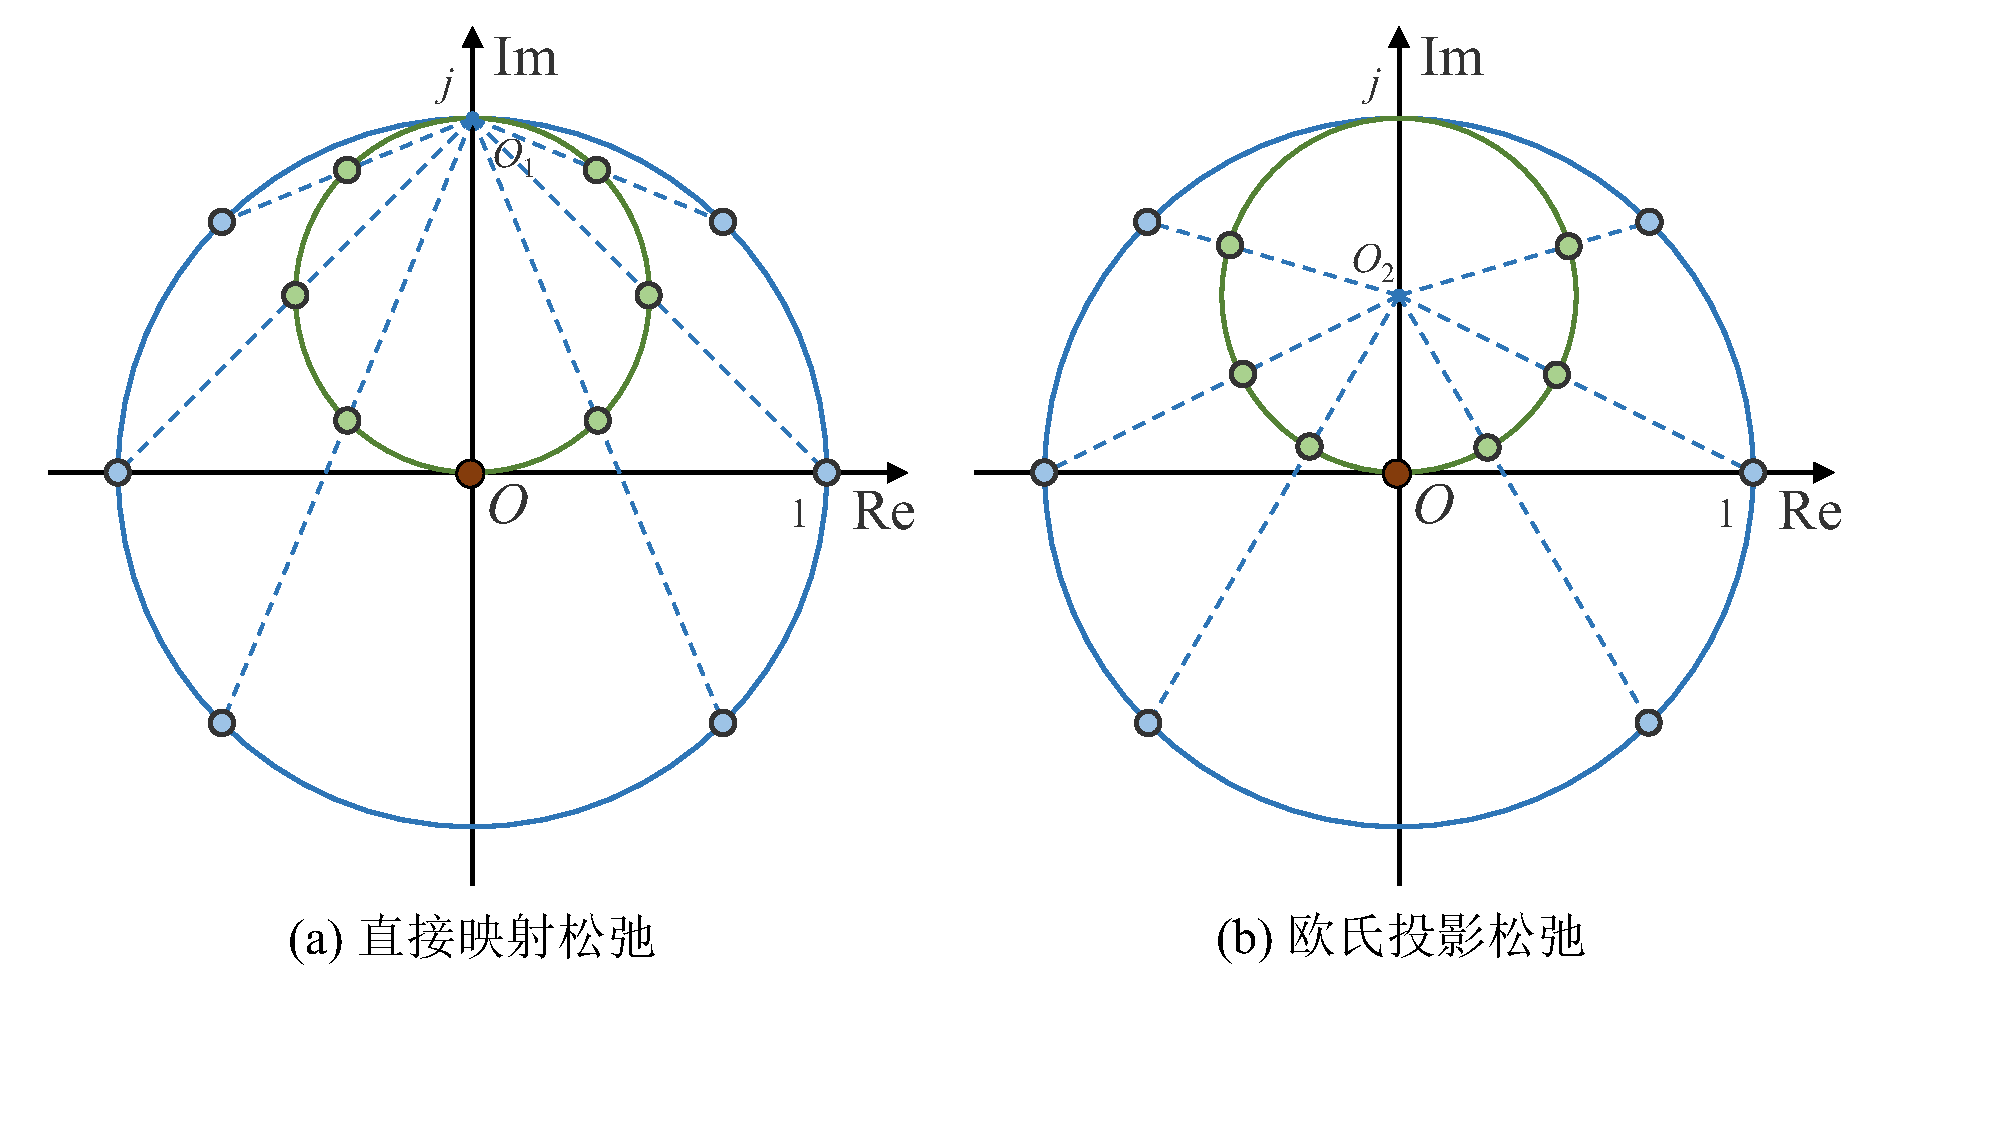
\includegraphics[width=0.8\linewidth]{cdma/cdma_relax.pdf}
	\caption{目前DMA研究中常用的松弛方法}
	\label{fig:cdma_relax}
\end{figure}

这两种方法都是对单位圆下的解进行变换得到的，单位圆约束由典型的采用单位幅度移相器的相控阵实现，此时，移相器所需设置的角度可以表示为$\theta_{i,l}=-\arg(g_{i,l} h_{i,l})$，即图中的蓝点所表示的位置。
直接松弛映射令DMA单元的可调相位参数$\phi_{i,l}^{\text{direct}}=\theta_{i,l}$，这种方法在几何上相当于将单位圆上的解直接缩放到洛伦兹圆上，不会改变DMA元素之间的相位差，从图~\ref{fig:cdma_relax}(a)中来看，这种映射是均匀的，其延长线相交于复平面上的$(0,j)$点处。
而对于欧氏投影松弛，其目标是在洛伦兹约束的可行域内寻找一个点$q_{i,l}$，使其与单位圆上的解$e^{j\theta_{i,l}}$在复平面上的欧氏距离最小。该问题可以表述为：
\begin{equation}
	\phi_{i,l}^{\text{proj}} = \mathop{\arg \min}_{\phi} \left| \frac{j+e^{j\phi}}{2} - e^{j\theta_{i,l}} \right|^2.
\end{equation}
从几何角度看，如图~\ref{fig:cdma_relax}(b)，欧氏投影解对应于单位圆上的最优解点与洛伦兹圆圆心$O_2$的连线与洛伦兹圆的交点。
根据几何关系，容易得出该映射对应的相位计算公式为：
\begin{equation}\label{eq:cdma_phi_proj}
	\phi_{i,l}^{\text{proj}} = \operatorname{\arctan 2}(\frac{2\sin\theta_{i,l}-1}{2}, \cos\theta_{i,l}).
\end{equation}
为了定量刻画两种方法与最优相位配置方法之间的性能差异，有必要进一步推导这两种松弛算法下DMA系统的平均信噪比表达式，并与定理~\ref{the:cdma_gamma}中的结果进行对比分析。

\begin{corollary}\label{cor:cdma_gamma_relax}
	在直接映射松弛下，假设DMA阵列与用户之间仍服从瑞利衰落信道$\bm g \sim \mathcal{CN}(\bm 0_{N\times1}, \sigma_g^2 \bm I_N)$，则系统的平均信噪比为：
	\begin{equation}\label{eq:cdma_gamma_relax}
		\gamma^{\mathrm{direct}} =
		\frac{P_{t}\sigma_g^2 N_d}{16\sigma^2 N_e}
		\left[\pi a_1^2 + (8-\pi) a_2\right],
	\end{equation}
	其中 $a_1$ 和 $a_2$ 的定义与定理~\ref{the:cdma_gamma}一致。
\end{corollary}

\begin{proof}
	在直接松弛下，DMA单元的幅度被固定为常数，而相位仅在单位圆约束下进行优化。其核心目标通常是最大化$\left| \sum_{l=1}^{N_e} g_{i,l} h_{i,l} e^{j\phi_{i,l}} \right|$，即令$\phi_{i,l}^{\mathrm{direct}} = -\arg(g_{i,l}h_{i,l})$。
	按照与定理~\ref{the:cdma_gamma}类似的推导步骤，此时单条波导上的有效信道增益变为：
	\begin{equation}
		Y_i= \frac{1}{2} \Big ( \underbrace{j \sum_{l=1}^{N_e} g_{i,l} h_{i,l}}_{T_1} + \underbrace{\sum_{l=1}^{N_e} |g_{i,l} h_{i,l}|}_{T_2} \Big ).
	\end{equation}
	对$|Y_i|^2$展开并取期望时，需要考虑复数项$T_1$和实数项$T_2$之间的相位关系。显然$T_1$是一个复高斯随机变量，其相位$\varphi_i = \arg(T_1)$在$[0, 2\pi)$上服从均匀分布，且相对于$T_2$具有统计独立性。对$|Y_i|^2$进行展开，有：
	\begin{equation}\label{eq:cdma_Yi2_relax}
		|Y_i|^2 = \frac{1}{4} \left( |T_1|^2 + T_2^2 + 2|T_1|T_2 \cos\varphi_i \right).
	\end{equation}
	在求取期望$\mathbb{E}(|Y_i|^2)$ 时，前两项的期望对应于定理~\ref{the:cdma_gamma}证明过程中一致。由于$\mathbb{E}(\cos\varphi_i) = 0$，第三项的期望为0，因此，直接映射松弛下的平均增益仅由式~\eqref{eq:cdma_Yi2_relax}的前两项构成，可得到式~\eqref{eq:cdma_gamma_relax}，证毕。
\end{proof}

\begin{corollary}\label{cor:cdma_gamma_proj}
	在欧氏投影松弛下，假设DMA阵列与用户之间仍服从瑞利衰落信道$\bm g \sim \mathcal{CN}(\bm 0_{N\times1}, \sigma_g^2 \bm I_N)$，则系统的平均信噪比为：
	\begin{equation}\label{eq:cdma_gamma_proj}
		\gamma^{\mathrm{proj}} = 
		\frac{P_t \sigma_g^2 N_d}{16 \sigma^2 N_e} 
		\left[ \pi \xi_2^2 (a_1^2-a_2) + 8\xi_1 a_2 \right],
	\end{equation}
	其中 $a_1$ 和 $a_2$ 的定义与定理~\ref{the:cdma_gamma}一致，$\xi_1$和$\xi_2$分别为欧氏投影下的能量修正因子和相位效率因子，其解析表达式如下：
	\begin{align}
		\xi_1 &=1 + \frac{1}{\pi} \left[ K(\frac{2\sqrt{2}}{3}) - 3 E(\frac{2\sqrt{2}}{3}) \right]\approx 0.741,\\
		\xi_2 &= \frac{1}{2\pi} \left[ K(\frac{2\sqrt{2}}{3}) + 3 E(\frac{2\sqrt{2}}{3}) \right] \approx 0.934,
	\end{align}
	其中$K(\cdot)$为第一类完全椭圆积分，$E(\cdot)$为第二类完全椭圆积分。
\end{corollary}

\begin{proof}
	在欧氏投影松弛中，相位配置依据最小化复平面距离准则，$\phi_{i,l}$ 由式~\eqref{eq:cdma_phi_proj}给出。
	定义单条波导上第$l$个单元的有效信道增益项为$u_{i,l} = g_{i,l} h_{i,l} q_{i,l}$。记$g_{i,l} h_{i,l} = |g_{i,l} h_{i,l}| e^{-j\theta_{i,l}}$，将欧氏投影的几何关系代入$q_{i,l}$，可以求得$u_{i,l}$的实部项和虚部分别为：
	\begin{align}
		\Re(u_{i,l}) &= \frac{|g_{i,l} h_{i,l}|}{2} \left( \sin\theta_{i,l} + \frac{1 - 0.5\sin\theta_{i,l}}{\sqrt{1.25 - \sin\theta_{i,l}}} \right), \\
		\Im(u_{i,l}) &= \frac{|g_{i,l} h_{i,l}|}{2} \cos\theta_{i,l}\cdot \left( 1 - \frac{0.5}{\sqrt{1.25 - \sin\theta_{i,l}}} \right).
	\end{align}
	单个增益项的功率$|u_{i,l}|^2=(\Re(u_{i,l}))^2+(\Im(u_{i,l}))^2$可利用上式计算为：
	\begin{equation}
		|u_{i,l}|^2 
		= \frac{|g_{i,l}h_{i,l}|^2}{4} \left(2 + \frac{2\sin\theta_{i,l} - 1}{\sqrt{1.25 - \sin\theta_{i,l}}}\right).
	\end{equation}
	考虑单条波导的总功率增益期望$\mathbb{E}[|Y_i|^2]$，将其展开，有：
	\begin{align}
		\mathbb{E}[|Y_i|^2] 
		&= \sum_{l=1}^{N_e} \mathbb{E}[|u_{i,l}|^2] + \sum_{l \neq k} \mathbb{E}[u_{i,l} u_{i,k}^*] \\
		&\overset{\text{(a)}}{=} \sigma_g^2 \mathbb{E}[|q_{i,l}|^2] \sum_{l=1}^{N_e} |h_{i,l}|^2 
		+ \sum_{l \neq k} \mathbb{E}[\Re(u_{i,l})] \mathbb{E}[\Re(u_{i,k})]
		\\
		&= 0.5\sigma_g^2 \xi_1 \sum_{l=1}^{N_e} |h_{i,l}|^2 
		+ \frac{\pi \sigma_g^2 \xi_2^2}{16}
		\cdot \left[ \left( \sum_{l=1}^{N_e} |h_{i,l}| \right)^2 - \sum_{l=1}^{N_e} \left(|h_{i,l}| \right)^2 \right],
	\end{align}
	其中(a)成立是因为$\mathbb{E}[\Im(u_{i,l})]=0$，$\xi_1$、$\xi_2$定义如下：
	\begin{align}
		\xi_1&=\mathbb{E}\left(1 + \frac{\sin\theta - 0.5}{\sqrt{1.25 - \sin\theta}}\right)
		= 1+\frac{1}{2\pi}\int_{0}^{2\pi} \frac{\sin\theta - 0.5}{\sqrt{1.25 - \sin\theta}}  d\theta, \\
		\xi_2&=\mathbb{E}\left( \sin\theta + \frac{1 - 0.5\sin\theta}{\sqrt{1.25 - \sin\theta}} \right)
		=\frac{1}{2\pi} \int_{0}^{2\pi} \frac{1 - 0.5\sin\theta}{\sqrt{1.25 - \sin\theta}}  d\theta.
	\end{align}
	
	$\xi_1$、$\xi_2$没有初等形式的解，利用代数变换可以将它们用第一类完全椭圆积分$K(k)$和第二类完全椭圆积分$E(k)$表达，利用换元法，记：
	\begin{align}
		\mathcal{J}_1 &= \int_{0}^{2\pi} \frac{d\theta}{\sqrt{a - \sin\theta}} = \frac{4}{\sqrt{a+1}} K\left(\sqrt{\frac{2}{a+1}}\right),\\
		\mathcal{J}_2 &= \int_{0}^{2\pi} \sqrt{a - \sin\theta} \, d\theta = 4\sqrt{a+1} E\left(\sqrt{\frac{2}{a+1}}\right).
	\end{align}
	代入$a=1.25$，可得$\mathcal{J}_1=\frac{8}{3} K(\frac{2\sqrt{2}}{3}),\;\mathcal{J}_2=6 E(\frac{2\sqrt{2}}{3})$。
	$\xi_1$、$\xi_2$可以使用$\mathcal{J}_1$、$\mathcal{J}_2$表示为：
	\begin{equation}
		\xi_1 = 1 + \frac{1}{2\pi}\left( \frac{3\mathcal{J}_1}{4}-\mathcal{J}_2\right) ,\quad
		\xi_2 = \frac{1}{2\pi}\left(\frac{3}{8}\mathcal{J}_1 +\frac{1}{2}\mathcal{J}_2\right).
	\end{equation}
	
	整理合并同类项，即可得到式~\eqref{eq:cdma_gamma_proj}，证毕。
\end{proof}

以直接映射松弛的平均信噪比$\gamma^{\mathrm{direct}}$为基准，定义归一化性能比值$R(N_e) = \gamma / \gamma^{\mathrm{direct}}$。当波导上的辐射单元数量趋于无穷时，由波导衰减引起的求和项之比的极限满足：
\begin{equation}\label{eq:cdma_a1a2_infty}
	\lim_{N_e \to \infty} \frac{a_2}{a_1^2} = \frac{(1 - e^{-\alpha D})^2}{1 - e^{-2\alpha D}} = \frac{1 - e^{-\alpha D}}{1 + e^{-\alpha D}} = \tanh\left(\frac{\alpha D}{2}\right).
\end{equation}
由定理~\ref{the:cdma_gamma}、推论~\ref{cor:cdma_gamma_relax}、推论~\ref{cor:cdma_gamma_proj}与式~\eqref{eq:cdma_a1a2_infty}，可推导出最优相位配置与欧氏投影松弛的渐近归一化性能：
\begin{align}
	R_{\infty}^{\mathrm{opt}} &= 1 + \frac{2\pi \sqrt{\tanh\left(\frac{\alpha D}{2}\right)}}{\pi + (8-\pi) \tanh\left(\frac{\alpha D}{2}\right)}, \label{eq:cdma_R_opt_inf}\\
	R_{\infty}^{\mathrm{proj}} &= \frac{\pi \xi_2^2 + (8 \xi_1 - \pi \xi_2^2) \tanh\left(\frac{\alpha D}{2}\right)}{\pi + (8-\pi) \tanh\left(\frac{\alpha D}{2}\right)}. \label{eq:cdma_R_proj_inf}
\end{align}

式~\eqref{eq:cdma_R_opt_inf}表明，最优相位配置相对于直接映射的增益并不会随$N_e$的增加而消失，而是收敛于大于$1$的常数。在 $\alpha D \ll 1$的条件下，$\tanh(\alpha D/2) \to 0$，非相干项 $a_2$可以忽略不计，系统的渐近归一化性能主要由相干增益项主导。
基于此近似，表~\ref{tab:cdma_comparison}提取了三种方法平均信噪比表达式中的主导项系数，并以直接映射松弛为基准进行了归一化比较。

\begin{table}[!htbp]
	\centering
	\caption{三种相位配置方法的相干增益性能对比}
	\label{tab:cdma_comparison}
	\begin{tabular}{cccc}
		\toprule
		\textbf{方法} & \textbf{映射策略} & \textbf{主导相干增益} & \textbf{渐近归一化性能} \\
		\midrule
		最优相位配置 & 式~\eqref{eq:cdma_phi_star} & $\pi a_1^2 + 2\pi a_1\sqrt{a_2}$ & $1+\sqrt{2\alpha D}$ \\
		直接映射松弛 & $\phi = -\arg(gh)$ & $\pi a_1^2$ & $1$ \\
		欧氏投影松弛 & 式~\eqref{eq:cdma_phi_proj} & $\pi \xi_2^2 a_1^2$ & $0.873$ \\
		\bottomrule
	\end{tabular}
\end{table}

通过对比可以看出，三种方法的平均性能满足最优相位配置$\gamma>$直接映射松弛$\gamma^{\mathrm{direct}}>$欧氏投影松弛$\gamma^{\mathrm{proj}}$。最优相位配置方法通过充分利用洛伦兹约束的固有偏置，保留了直接映射松弛所忽略的交叉项增益，在性能上严格优于后者。特别是在$N_e$较小时，这种相干增益在总能量中占比较大，最优配置方法的优势将更为显著。
而欧氏投影松弛虽在几何上最小化了单元层面的映射误差，却因引入额外的相位失配导致了约$12.7\%$的功率衰减，其有效相干增益反而低于直接映射松弛。


\subsection{非完美CSI下的平均信噪比分析}

在实际通信场景中，受限于信道估计误差、反馈时延以及硬件不完美等因素，基站通常难以获取精确的信道状态信息。本小节基于统计信道误差模型，分析非完美CSI对所提最优相位配置方法性能的影响，并推导此时系统的平均信噪比闭式解。

假设实际信道向量$\bm g$可分解为估计信道$\hat{\bm g}$与估计误差$\tilde{\bm g}$之和，即：
\begin{equation}\label{eq:cdma_channel_model_imp}
	\bm g = \hat{\bm g} + \tilde{\bm g},
\end{equation}
其中$\hat{\bm g} \sim \mathcal{CN}(\bm 0, \hat{\sigma}_g^2 \bm I_N)$，$\tilde{\bm g} \sim \mathcal{CN}(\bm 0, \tilde{\sigma}_g^2 \bm I_N)$，且二者相互独立，实际信道增益方差为$\sigma_g^2 = \hat{\sigma}_g^2 + \tilde{\sigma}_g^2$。

在非完美CSI条件下，系统基于估计信道$\hat{\bm g}$设计相位配置矩阵$\bm Q(\hat{\bm g})$ 及预编码器$\bm{w}(\hat{\bm{g}})$，而接收信噪比则由实际信道$\bm g$决定。因此，系统的平均信噪比可表示为：
\begin{equation}\label{eq:cdma_gamma_imp_def}
	\gamma^{\mathrm{imp}} = \frac{P_{t}}{\sigma^2}\mathbb{E}(\left| \bm g^\mathrm{T} \bm H \bm Q \bm w \right|^2)
	= \frac{P_{t}}{\sigma^2} \left[\mathbb{E}( \left| \bm{\hat{g}}^\mathrm{T} \bm H \bm Q \bm w \right|^2 )
	+ \mathbb{E}( \left| \bm{\tilde{g}}^\mathrm{T} \bm H \bm Q \bm w \right|^2 )\right].
\end{equation}

上式中括号内第一项$\mathbb{E}( \left| \bm{\hat{g}}^\mathrm{T} \bm H \bm Q \bm w \right|^2 )$可直接利用定理~\ref{the:cdma_gamma}的结论，只需将原表达式中的信道方差 $\sigma_g^2$替换为估计信道方差$\hat{\sigma}_g^2$，即可得到该项的表达式：
\begin{equation}\label{eq:cdma_term1_imp}
	\mathbb{E}( \left| \bm{\hat{g}}^\mathrm{T} \bm H \bm Q \bm w \right|^2 ) = \frac{\hat{\sigma}_g^2 N_d}{16 N_e}\left[\pi a_1^2 + 2\pi a_1\sqrt{a_2} + (8-\pi) a_2\right].
\end{equation}

接下来分析第二项$\mathbb{E}( \left| \bm{\tilde{g}}^\mathrm{T} \bm H \bm Q \bm w \right|^2 )$，这是一个由信道估计误差引起的干扰项。根据重期望公式$\mathbb{E}(X) = \mathbb{E}_Y[\mathbb{E}_X(X|Y)]$，通过先对$\tilde{\bm g}$求期望，再对$\hat{\bm g}$求期望，可得：
\begin{align}\label{eq:cdma_term2_expand}
	\mathbb{E}( \left| \bm{\tilde{g}}^\mathrm{T} \bm H \bm Q \bm w \right|^2 ) &= \mathbb{E}_{\hat{\bm g}}\left[ \mathbb{E}_{\tilde{\bm g}}\left( \bm w^\mathrm{H} \bm Q^\mathrm{H} \bm H^\mathrm{H} \tilde{\bm g}^* \tilde{\bm g}^\mathrm{T} \bm H \bm Q \bm w \mid \hat{\bm g} \right) \right] \\
	&\overset{\text{(a)}}{=} \mathbb{E}_{\hat{\bm g}}\left[ \bm w^\mathrm{H} \bm Q^\mathrm{H} \bm H^\mathrm{H} \mathbb{E}_{\tilde{\bm g}}(\tilde{\bm g}^* \tilde{\bm g}^\mathrm{T}) \bm H \bm Q \bm w \right] \\
	&\overset{\text{(b)}}{=} \tilde{\sigma}_g^2 \mathbb{E}_{\hat{\bm g}}\left( \|\bm H \bm Q \bm w\|^2 \right),
\end{align}
其中(a)成立是因为在内部的期望中，$\hat{\bm g}$被视为已知，那么基于它计算出来的$\bm Q$和$\bm w$为常量矩阵，(b)成立是因为$\mathbb{E}_{\tilde{\bm g}} \left( \bm{\tilde{g}}^* \bm{\tilde{g}}^\mathrm{T} \right) = \tilde{\sigma}_g^2 \bm{I}_N$。利用矩阵$\bm H$和$\bm Q$的块对角结构，范数项可展开为：
\begin{equation}
	\|\bm H \bm Q \bm w\|^2 = \sum_{i=1}^{N_d} \left( |w_i|^2 \sum_{l=1}^{N_e} |h_{i,l}|^2 |q_{i,l}|^2\right).
\end{equation}

考虑到预编码向量满足功率约束$\|\bm w\|^2 = 1$，且各波导的统计特性一致，上述求和项可简化为单条波导内各单元功率增益之和，因此，其期望可写为：
\begin{equation}\label{eq:cdma_EHQw2}
	\mathbb{E}_{\hat{\bm g}}\left( \|\bm H \bm Q \bm w\|^2 \right) = \sum_{l=1}^{N_e} |h_{i,l}|^2 \cdot \mathbb{E}(|q_{i,l}|^2).
\end{equation}
对于满足洛伦兹约束的单元响应，其模平方为$|q_{i,l}|^2 = (1+\sin\phi_{i,l})/2$。由于最优相位$\phi_{i,l}$跟随随机信道相位变化，其在$[0, 2\pi)$内服从均匀分布，于是：
\begin{equation}\label{eq:cdma_Eqil2}
	\mathbb{E}(|q_{i,l}|^2) = \frac{1}{2}+\frac{1}{2}\mathbb{E}(\sin\phi_{i,l})
	=\frac{1}{2}.
\end{equation}
结合式~\eqref{eq:cdma_hil}定义的波导衰减模型，将式~\eqref{eq:cdma_EHQw2}和式~\eqref{eq:cdma_Eqil2}代入式~\eqref{eq:cdma_term2_expand}，有：
\begin{equation}\label{eq:cdma_term2_imp}
	\mathbb{E}( \left| \bm{\tilde{g}}^\mathrm{T} \bm H \bm Q \bm w \right|^2 ) 
	= \tilde{\sigma}_g^2 \sum_{l=1}^{N_e} \frac{1}{N_e} e^{-2\alpha D(l-1)} \cdot \frac{1}{2} 
	= \frac{\tilde{\sigma}_g^2}{2N_e} \frac{1 - e^{-2\alpha D N_e}}{1 - e^{-2\alpha D}}.
\end{equation}
综合式~\eqref{eq:cdma_term1_imp}与式~\eqref{eq:cdma_term2_imp}，可得非完美CSI下系统平均信噪比的闭式解，如推论~\ref{cor:cdma_gamma_imp}所示。

\begin{corollary}\label{cor:cdma_gamma_imp}
	在存在信道估计误差且满足式~\eqref{eq:cdma_channel_model_imp}所示的统计误差模型下，定义相对信道估计误差系数$\xi$为误差方差与实际信道方差之比，即：$\xi = \frac{\tilde{\sigma}_g^2}{\sigma_g^2}, \; \xi \in [0, 1]$，则DMA通信系统的平均信噪比为：
	\begin{equation}
		\gamma^{\mathrm{imp}} = (1-\xi)\frac{P_{t}\sigma_g^2 N_d}{16\sigma^2 N_e}\left[\pi a_1^2 + 2\pi a_1\sqrt{a_2} + (8-\pi) a_2\right] 
		+ \xi \frac{P_t \sigma_g^2 a_2}{2 \sigma^2 N_e},
	\end{equation}
	其中$a_1, a_2$的定义同定理~\ref{the:cdma_gamma}。
\end{corollary}

推论~\ref{cor:cdma_gamma_imp}表明，非完美CSI下的平均信噪比由两部分组成：第一部分由估计信道的质量$\hat{\sigma}_g^2$主导，其增益随天线数量$N$的增加而显著增长，体现了DMA的波束赋形增益；第二部分由信道估计误差$\tilde{\sigma}_g^2$引起，该项不仅没有波束赋形增益，反而引入了与波导衰减有关的因子。
权重因子由信道估计质量$\xi$决定，当$\xi \to 0$时，信道估计趋于完美，推论~\ref{cor:cdma_gamma_imp}退化为定理~\ref{the:cdma_gamma}中的完美CSI结果；当$\xi \to 1$，即完全无法估计信道时，系统性能仅剩由波导结构决定的固定功率泄露。
值得注意的是，该误差项与波导数量$N_d$无关，这表明随着阵列规模$N_d$的增加，虽然由估计误差引起的误差项保持不变，但波束赋形增益项会随$N_d$线性增长。因此，增加波导数量可以在一定程度上弥补由CSI不完美带来的性能损失。


\subsection{中断概率和遍历容量分析}

基于前文推导的最优相位配置方法及平均信噪比闭式解，本节将进一步分析系统的可靠性与频谱效率，分别推导DMA系统的中断概率和遍历容量。为了便于后续性能指标的推导，首先需确定接收端瞬时信噪比的统计分布特性。在最优配置下，如前文所述，有效信道增益主要由 $N_d$个独立波导的增益之和构成。
根据中心极限定理，当DMA阵列较大时，$\left| \bm g^\mathrm{T} \bm H \bm Q \bm w \right|$近似服从高斯分布，因此瞬时信噪比可近似通过伽马分布进行建模。
设瞬时信噪比服从形状参数为$k$、尺度参数为$\theta$的伽马分布，其概率密度函数为：
\begin{equation}\label{eq:cdma_pdf_gamma}
	f_{\mathrm{SNR}}(x) = \frac{x^{k-1} e^{-\frac{x}{\theta}}}{\Gamma(k) \theta^k}, \quad x \geq 0,
\end{equation}
其中$\Gamma(\cdot)$是伽马函数。为了确定伽马分布的参数$k$和$\theta$，除了已知的一阶矩$\mathbb{E}(\mathrm{SNR})$，还需要推导信噪比的方差$\operatorname{Var}(\mathrm{SNR})$。由于各波导间是独立的，总方差为各波导信噪比方差之和，即：
\begin{equation}\label{eq:cdma_var_snr}
	\operatorname{Var}(\mathrm{SNR}) = \left(\frac{P_t}{\sigma^2}\right)^2 \sum_{i=1}^{N_d} \operatorname{Var}(|Y_i|^2),
\end{equation}
其中$Y_i$为单条波导的有效信道增益。


在最优相位配置下，单条波导的有效信道增益模值可表示为两部分之和：$|Y_i| = \frac{1}{2} (X_1 + X_2)$，其中相干项 $X_1 = \left| \sum_{l=1}^{N_e} g_{i,l} h_{i,l} \right|$，非相干项 $X_2 = \sum_{l=1}^{N_e} |g_{i,l} h_{i,l}|$。
首先分别分析 $X_1$ 和 $X_2$ 的统计特性。对于 $X_1$，其内部复数和服从零均值复高斯分布 $\mathcal{CN}\left(0, \frac{\sigma_g^2 a_2}{N_e}\right)$，因此 $X_1$ 服从瑞利分布，其均值和方差分别为：
\begin{equation}
	\mu_{X_1} = \frac{\sqrt{\pi} \sigma_g \sqrt{a_2}}{2 \sqrt{N_e}}, \quad \sigma_{X_1}^2 = \frac{(4-\pi)\sigma_g^2 a_2}{4 N_e};
\end{equation}
对于 $X_2$，它是大量独立瑞利随机变量之和。根据中心极限定理，当 $N_e$ 较大时，$X_2$ 渐近服从高斯分布$\mathcal{N}(\mu_{X_2}, \sigma_{X_2}^2)$，其均值和方差分别为：
\begin{equation}
	\mu_{X_2} = \frac{\sqrt{\pi} \sigma_g a_1}{2 \sqrt{N_e}}, \quad \sigma_{X_2}^2 = \frac{(4-\pi)\sigma_g^2 a_2}{4 N_e},
\end{equation}
其中$a_1 = \frac{1 - e^{-\alpha D N_e}}{1 - e^{-\alpha D}}$，$a_2 = \frac{1 - e^{-2\alpha D N_e}}{1 - e^{-2\alpha D}}$。

如定理~\ref{the:cdma_gamma}证明中所述，当 $N_e$ 较大时，$X_1$ 和 $X_2$ 近似统计独立。因此，有效信道增益模值 $|Y_i| = \frac{1}{2}(X_1 + X_2)$ 的均值 $\mu_Y$ 和方差 $\sigma_Y^2$ 可直接求得：
\begin{align}
	\mu_Y &= \frac{1}{2}(\mu_{X_1} + \mu_{X_2}) = \frac{\sqrt{\pi} \sigma_g}{4 \sqrt{N_e}}(a_1 + \sqrt{a_2}), \\
	\sigma_Y^2 &= \frac{1}{4}(\sigma_{X_1}^2 + \sigma_{X_2}^2) = \frac{(4-\pi)\sigma_g^2 a_2}{8 N_e}.
\end{align}

由于非相干项 $X_2$ 具有较大的均值且渐近服从高斯分布，它主导了 $|Y_i|$ 的分布形态，故可近似认为 $|Y_i|$ 渐近服从高斯分布 $\mathcal{N}(\mu_Y, \sigma_Y^2)$。
对于服从高斯分布的幅度变量 $|Y_i|$，其平方的方差可由矩的关系导出：
\begin{equation}\label{eq:cdma_var_Yi2}
	\operatorname{Var}(|Y_i|^2) = 4\mu_Y^2 \sigma_Y^2 + 2\sigma_Y^4.
\end{equation}
将 $\mu_Y$ 和 $\sigma_Y^2$ 代入式~\eqref{eq:cdma_var_Yi2}，整理可得单条波导增益平方的方差：
\begin{equation}
	\operatorname{Var}(|Y_i|^2) = \frac{(4-\pi)\sigma_g^4 a_2}{32 N_e^2} \left[ \pi(a_1 + \sqrt{a_2})^2 + (4-\pi)a_2 \right].
\end{equation}

将上式代回式~\eqref{eq:cdma_var_snr}，可得系统总信噪比的方差：
\begin{equation}\label{eq:cdma_var_snr_output}
	\operatorname{Var}(\mathrm{SNR}) = 
	\frac{(4-\pi) P_t^2 \sigma_g^4 N_d a_2}{32 \sigma^4 N_e^2} \left[ \pi(a_1 + \sqrt{a_2})^2 + (4-\pi)a_2 \right].
\end{equation}

结合定理~\ref{the:cdma_gamma}中推导的平均信噪比 $\mathbb{E}(\mathrm{SNR})$，利用矩匹配法，即可唯一确定伽马分布的形状参数 $k$ 和尺度参数 $\theta$ 如下：
\begin{align}\label{eq:cdma_gamma_k_theta}
	k &= \frac{(\mathbb{E}(\mathrm{SNR}))^2}{\operatorname{Var}(\mathrm{SNR})}
	= \frac{N_d [\pi a_1^2 + 2\pi a_1\sqrt{a_2} + (8-\pi)a_2]^2}{8(4-\pi)a_2 \left[ \pi(a_1+\sqrt{a_2})^2 + (4-\pi)a_2 \right]}, \\
	\theta &= \frac{\operatorname{Var}(\mathrm{SNR})}{\mathbb{E}(\mathrm{SNR})}
	= \frac{P_t \sigma_g^2 a_2 (4-\pi) \left[ \pi(a_1+\sqrt{a_2})^2 + (4-\pi)a_2 \right]}{2 \sigma^2 N_e [\pi a_1^2 + 2\pi a_1\sqrt{a_2} + (8-\pi)a_2]}.
\end{align}


\subsubsection{中断概率}

中断概率是衡量通信系统可靠性的重要指标，定义为瞬时SNR低于特定目标阈值$\gamma_{\text{th}}$的概率。基于上述伽马分布模型，系统的中断概率$P_{\text{out}}$可表示为：
\begin{equation}
	P_{\text{out}}= \operatorname{Pr}(\mathrm{SNR} < \gamma_{\text{th}}) = \int_{0}^{\gamma_{\text{th}}} f_{\mathrm{SNR}}(\gamma)\, d\gamma.
\end{equation}
将式~\eqref{eq:cdma_pdf_gamma}代入积分，并作变量代换$t = x/\theta$，得：
\begin{equation}
	P_{\text{out}} 
	= \int_{0}^{\gamma_{\text{th}}} \frac{x^{k-1} e^{-\frac{x}{\theta}}}{\Gamma(k) \theta^k} \, dx
	= \frac{1}{\Gamma(k)} \int_{0}^{\frac{\gamma_{\text{th}}}{\theta}} t^{k-1} e^{-t}\, dt 
	= \frac{\gamma_{\text{inc}}\left(k, \frac{\gamma_{\text{th}}}{\theta}\right)}{\Gamma(k)},
\end{equation}
其中$\gamma_{\text{inc}}(s, x) = \int_0^x t^{s-1} e^{-t}\, dt$为下不完全伽马函数。考虑到$\theta = \gamma / k$，中断概率可表示为：
\begin{equation}\label{eq:cdma_Pout_final}
	P_{\text{out}} = \frac{\gamma_{\text{inc}}\left(k, \frac{k \gamma_{\text{th}}}{\gamma}\right)}{\Gamma(k)}.
\end{equation}
式~\eqref{eq:cdma_Pout_final}表明，在给定的阈值下，中断性能主要取决于平均信噪比$\gamma$（由定理~\ref{the:cdma_gamma}给出）以及反映DMA阵列固有特性的形状参数 $k$。

\subsubsection{遍历容量}

遍历容量表征了DMA系统的平均频谱效率，定义为瞬时互信息的期望值：
\begin{equation}\label{eq:cdma_capacity_def}
	C = \mathbb{E}\left[ \log_2(1 + \mathrm{SNR}) \right] = \int_{0}^{\infty} \log_2(1 + x) f_{\mathrm{SNR}}(x)\, dx.
\end{equation}
上式的积分难以直接求解，本小节将通过推导容量的紧致上界、高信噪比以及低信噪比下的渐近近似，来分析系统的频谱效率特性。根据Jensen不等式，可得遍历容量的上界：
\begin{equation}
	C \leq C^{\text{up}} = \log_2\left( 1 + \mathbb{E}(\mathrm{SNR}) \right) = \log_2(1 + \gamma).
\end{equation}
将定理~\ref{the:cdma_gamma}中推导的平均信噪比$\gamma$代入，可得：
\begin{equation}
	\label{eq:cdma_capacity_upper}C^{\text{up}} = \log_2\left( 1 + \frac{P_{t}\sigma_g^2 N_d}{16\sigma^2 N_e}\left[\pi a_1^2 + 2\pi a_1\sqrt{a_2} + (8-\pi) a_2\right] \right).
\end{equation}
上式表明，遍历容量上界随发射功率$P_t$对数增长。在大规模DMA系统中，由于大量辐射单元的叠加作用使得信噪比的方差相对于均值逐渐减小，该上界非常紧致，足以作为系统容量评估的有效近似。

为了进一步量化参数$k$对容量的影响，下面考虑低信噪比场景和高信噪比场景下的近似。
在低SNR区域，利用泰勒级数展开，遍历容量可近似为：
\begin{equation}
	C = \frac{1}{\ln 2} \mathbb{E}\left[ \ln(1 + \mathrm{SNR}) \right]
	\approx \frac{1}{\ln 2} \left( \mathbb{E}(\mathrm{SNR}) - \frac{1}{2}\mathbb{E}(\mathrm{SNR}^2) \right).
\end{equation}
其中二阶矩可计算为：$\mathbb{E}(\mathrm{SNR}^2)=(\mathbb{E}(\mathrm{SNR}))^2+\operatorname{Var}(\mathrm{SNR})$。代入$\mathbb{E}(\mathrm{SNR})=\gamma$和$\operatorname{Var}(\mathrm{SNR})=\gamma^2/k$，低信噪比下的近似遍历容量为：
\begin{equation}\label{eq:cdma_capacity_low_snr}
	C^{\text{low}} \approx \frac{\gamma}{\ln 2} - \frac{\gamma^2}{2 \ln 2} \left( 1 + \frac{1}{k} \right).
\end{equation}

在高信噪比下，遍历容量可近似表示为：
\begin{equation}
	C \approx \mathbb{E}\left[ \log_2(\mathrm{SNR}) \right] = \frac{1}{\ln 2} \mathbb{E}\left[ \ln(\mathrm{SNR}) \right].
\end{equation}
根据伽马分布的统计特性，其对数期望为：
\begin{equation}
	\mathbb{E}[\ln(\mathrm{SNR})] = \psi(k) + \ln(\theta),
\end{equation}
其中$\psi(x) = \frac{d}{dx}\ln \Gamma(x)$为双伽马函数。整理得到高SNR下遍历容量的渐近表达式：
\begin{equation}\label{eq:cdma_capacity_high_snr}
	C^{\text{high}}
	\approx \log_2(\gamma) + \frac{\psi(k) - \ln(k)}{\ln 2}.
\end{equation}


\section{基于RSSI的相位估计与相位对齐算法}

前文分析了在完美CSI条件下的最优相位配置及其性能上限。然而，在实际部署中，DMA阵列通常包含数以百计的辐射单元，受限于硬件成本和功耗，射频链路的数量$N_d$远小于辐射单元总数$N$。在这种架构下，基带处理单元通常只能获取每条波导叠加后的等效信道信息，而难以通过传统的导频训练方案单独估计每个辐射单元的信道系数$g_{i,l}h_{i,l}$。若采用开关轮询的方式逐个估计，导频开销将随$N_e$线性增长，导致系统传输效率下降。鉴于此，本节提出一种基于RSSI的相位对齐算法。由于用户端能够容易地测量下行链路的接收功率并反馈给基站，该方法无需单独估计信道，而是利用RSSI反馈直接优化DMA相位配置，从而最大化接收信噪比。

通过第~\ref{sec:cdma_opt}节的分析可知，在采用MRT预编码策略时，系统会根据各条波导的有效信道进行最大比合并，总接收功率表现为各个波导接收信号幅度的相干叠加，因此，可以分别对$N_d$个波导进行独立优化。
不失一般性，考虑第$i$条波导，目标是通过调整该波导上$N_e$个单元的相位配置$\bm q_i$，以最大化该波导贡献的接收功率。
令$u_{i,l} = \sqrt{P_t} g_{i,l} h_{i,l}$表示包含发射功率、空间信道和波导传播效应的复合信道增益，则第$i$条波导在用户端的接收功率可表示为：
\begin{equation}\label{eq:cdma_rssi_power_def}
	p(\bm{\phi}_i) = \left| \sum_{l=1}^{N_e} u_{i,l} \frac{j+e^{j\phi_{i,l}}}{2} + \eta \right|^2,
\end{equation}
其中$\bm{\phi}_i = [\phi_{i,1}, \cdots, \phi_{i,N_e}]^\mathrm{T}$为待优化的相位向量。由于噪声项$\eta$的存在，单次测量的功率具有随机性，但以接收功率期望最大化为目标等价于最大化有用信号功率。针对此类问题，坐标下降法提供了一种高效的求解思路。该方法通过迭代机制，将复杂的多变量联合优化问题分解为一系列单变量子问题，即在每一步迭代中仅优化一个辐射单元的相位，同时保持其余单元状态固定，从而逐步逼近最优解。为了构建该算法，首先需要分析在固定其他单元配置时，如何确定目标单元的相位，使得信号功率最大。

\subsection{功率期望最大化的相位估计方法}\label{sec:cdma_phase_est_method}

本小节考虑对第$i$条波导上第$\lambda$个单元的相位进行优化。固定除第$\lambda$单元以外的所有其他单元的相位$\{\phi_{i,l}\}_{l \neq \lambda}$，仅将当前单元的相位$\phi_{i,\lambda}$视为变量。
对式~\eqref{eq:cdma_rssi_power_def}中的可变量与不变量进行分离，令$T_1 =j\frac{u_{i,\lambda}}{2} + \sum_{l\neq \lambda} u_{i,l} \frac{j+e^{j\phi_{i,l}}}{2}, \; T_2=\frac{u_{i,\lambda}}{2}$，接收功率可表示为$p(\phi_{i,\lambda})=\left| T_1+T_2 e^{j\phi_{i,\lambda}}+\eta \right|^2 $。利用噪声$\eta \sim \mathcal{CN}(0, \sigma^2)$的统计特性，接收功率的期望可推导为：
\begin{align}
	\mathbb{E}[p(\phi_{i,\lambda})] &= |T_1 + T_2 e^{j\phi_{i,\lambda}}|^2 + \sigma^2 \\
	&=|T_1|^2 + |T_2|^2 + \sigma^2 +  2|T_1||T_2| \cos(\phi_{i,\lambda} - \psi),\label{eq:cdma_expected_power}
\end{align}
其中$\psi = \arg(T_1 T_2^*)$。式~\eqref{eq:cdma_expected_power}表明，功率的统计期望关于相位$\phi_{i,\lambda}$遵循周期为$2\pi$的余弦规律，$\phi_{i,\lambda}=\psi$为使得期望功率最大化的相位。因此，相位优化问题为一个余弦波参数估计问题：即通过有限次的含噪功率测量，估计出相位参数$\psi$。

为便于参数估计，将式~\eqref{eq:cdma_expected_power}展开为如下线性回归模型：
\begin{equation}\label{eq:cdma_linear_model}
	\mathbb{E}[p(\phi)] = x_0 + x_1 \cos\phi + x_2 \sin\phi,
\end{equation}
其中待估参数定义为$x_0 = |T_1|^2 + |T_2|^2 + \sigma^2$，$x_1 = 2|T_1||T_2| \cos\psi$，$x_2 = 2|T_1||T_2| \sin\psi$。
一旦获得参数$x_1$和$x_2$的可靠估计，目标相位即可由$\psi = \operatorname{atan2}(x_2, x_1)$确定。

为了从含噪观测中准确恢复上述参数，首先需要确定合适的相位采样策略。假设在区间$[0, 2\pi)$内选取$M$个相位采样点$\{\varphi_1, \varphi_2, \cdots, \varphi_M\}$，并测量对应的接收功率。根据式~\eqref{eq:cdma_linear_model}，测量过程可建模为如下线性观测方程：
\begin{equation}\label{eq:cdma_bmp}
	\bm{p} = \bm{A} \bm{x} + \bm{\epsilon},
\end{equation}
其中$\bm p=[p_1,\ldots,p_M]^\mathrm{T}$为观测向量，$\bm x=[x_0,x_1,x_2]^\mathrm{T}$为参数向量，$\bm\epsilon\in\mathbb{R}^{M\times 1}$是由噪声 $\eta$引起的测量误差，满足$E(\boldsymbol{\epsilon}) = \mathbf{0}$，可近似认为$\operatorname{Cov}(\boldsymbol{\epsilon})=\sigma_\epsilon^2\bm I$，$\bm A\in\mathbb{R}^{M\times 3}$为观测矩阵，其具体形式为：
\begin{equation}
	\bm A=
	\begin{bmatrix}
		1      & \cos\varphi_1 & \sin\varphi_1 \\
		\vdots & \vdots        & \vdots        \\
		1      & \cos\varphi_M & \sin\varphi_M
	\end{bmatrix}.
\end{equation}

根据最小二乘法，估计量的形式为：
\begin{equation}
	\hat{\bm{x}}
	= \mathop{\arg\min}_{\bm x} \|\bm{p} - \bm{A}{\bm{x}}\|^2
	= (\bm{A}^\mathrm{T} \bm{A})^{-1} \bm{A}^\mathrm{T} \bm{p}.
\end{equation}
代入式~\eqref{eq:cdma_bmp}，可得：
\begin{align}
	\hat{\bm{x}} 
	&= (\bm{A}^{\mathrm{T}} \bm{A})^{-1} \bm{A}^{\mathrm{T}} (\bm{A} \bm{x} + \bm{\epsilon}) \\
	&= (\bm{A}^{\mathrm{T}} \bm{A})^{-1} (\bm{A}^{\mathrm{T}} \bm{A}) \bm{x}
	+ (\bm{A}^{\mathrm{T}} \bm{A})^{-1} \bm{A}^{\mathrm{T}} \bm{\epsilon} = \bm{x} + (\bm{A}^{\mathrm{T}} \bm{A})^{-1} \bm{A}^{\mathrm{T}} \bm{\epsilon}.
\end{align}

这说明估计量$\hat{\bm x}$是无偏估计，记$\bm A^\dagger = (\bm{A}^{\mathrm{T}} \bm{A})^{-1} \bm{A}^{\mathrm{T}}$，则$\hat{\bm x}$的协方差矩阵计算为：
\begin{align}
	\operatorname{Cov}(\hat{\bm x})
	&= \mathbb{E}[(\hat{\bm x} - \mathbb{E}(\hat{\bm x}))(\hat{\bm x}- \mathbb{E}(\hat{\bm x}))^{\mathrm{T}}] 
	= \mathbb{E}\!\left[(\bm A^\dagger \bm\epsilon)(\bm A^\dagger \bm\epsilon)^{\mathrm T}\right] \\
	&= \operatorname{Cov}(\bm A^\dagger \bm\epsilon)
	=\bm A^\dagger \operatorname{Cov}(\bm\epsilon)(\bm A^\dagger)^{\mathrm T}
	= \sigma_\epsilon^2 \bm A^\dagger (\bm A^\dagger)^{\mathrm T},
\end{align}
式中$\bm A^\dagger (\bm A^\dagger)^{\mathrm T}$可计算为：
\begin{equation}
	\bm A^\dagger(\bm A^\dagger)^{\mathrm T}
	= (\bm A^{\mathrm T}\bm A)^{-1}\bm A^{\mathrm T}\bm A(\bm A^{\mathrm T}\bm A)^{-1}
	= (\bm A^{\mathrm T}\bm A)^{-1}.
\end{equation}

进一步地，定义估计均方误差为：
\begin{equation}
	\mathrm{MSE}(\hat{\bm x})
	= \mathbb{E}\!\left[\|\hat{\bm x}-\bm x\|^2\right]
	= \operatorname{tr}\!\left(\operatorname{Cov}(\hat{\bm x})\right)
	= \sigma_\epsilon^2 \operatorname{tr}\!\left((\bm A^{\mathrm T}\bm A)^{-1}\right).
\end{equation}
由此可见，在噪声方差固定的情况下，最小化参数估计的均方误差可表述为：
\begin{equation}
	\min_{\{\varphi_m\}} \operatorname{tr}\!\left((\bm A^{\mathrm T}\bm A)^{-1}\right), \quad \text{s.t.} \quad \varphi_m \in [0, 2\pi),\;\forall m. 
\end{equation}

计算一般形式下的信息矩阵 $\bm{F} = \bm{A}^\mathrm{T} \bm{A}$如下：
\begin{equation}
	\bm F = 
	\begin{bmatrix}
		M & \sum_{m=1}^M \cos\varphi_m & \sum_{m=1}^M \sin\varphi_m \\
		\sum_{m=1}^M \cos\varphi_m & \sum_{m=1}^M \cos^2\varphi_m & \sum_{m=1}^M \cos\varphi_m \sin\varphi_m \\
		\sum_{m=1}^M \sin\varphi_m & \sum_{m=1}^M \cos\varphi_m \sin\varphi_m & \sum_{m=1}^M \sin^2\varphi_m
	\end{bmatrix}.
\end{equation}
为方便后续分析，将矩阵$\bm{F}$进行分块表示如下：
\begin{equation}
	\bm F = 
	\begin{bmatrix}
		F_{11} & \bm f_{12}^{\mathrm T} \\
		\bm f_{12} & \bm F_{22}
	\end{bmatrix},
\end{equation}
其中：
\begin{equation}
	F_{11} = M,\;
	\bm f_{12} = \begin{bmatrix} \sum \cos\varphi_m \\ \sum \sin\varphi_m \end{bmatrix},\;
	\bm F_{22} = \begin{bmatrix} \sum \cos^2\varphi_m & \sum \cos\varphi_m \sin\varphi_m \\ \sum \cos\varphi_m \sin\varphi_m & \sum \sin^2\varphi_m \end{bmatrix}.
\end{equation}
定义$\bm{F}_{22}$在矩阵$\bm{F}$中的Schur补为$S = F_{11} - \bm{f}_{12}^{\mathrm{T}} \bm{F}_{22}^{-1} \bm{f}_{12}$，利用分块矩阵求逆公式，矩阵$\bm{F}$的逆可表示为：
\begin{equation}
	\bm{F}^{-1} =
	\begin{bmatrix}
		S^{-1} & -S^{-1} \bm{f}_{12}^{\mathrm{T}} \bm{F}_{22}^{-1} \\
		-\bm{F}_{22}^{-1}  \bm{f}_{12} S^{-1} & \bm{F}_{22}^{-1} + \bm{F}_{22}^{-1} \bm{f}_{12} S^{-1} \bm{f}_{12}^{\mathrm{T}} \bm{F}_{22}^{-1}
	\end{bmatrix}.
\end{equation}
于是，$\operatorname{tr}(\bm F^{-1})$可计算为：
\begin{align}
	\operatorname{tr}(\bm{F}^{-1}) &= S^{-1} + \operatorname{tr}\!\left( \bm{F}_{22}^{-1} + \bm{F}_{22}^{-1} \bm{f}_{12} S^{-1} \bm{f}_{12}^{\mathrm{T}} \bm{F}_{22}^{-1} \right) \\
	&= \frac{1}{S} + \operatorname{tr}(\bm{F}_{22}^{-1}) + \frac{1}{S} \operatorname{tr}\!\left( \bm{F}_{22}^{-1} \bm{f}_{12} \bm{f}_{12}^{\mathrm{T}} \bm{F}_{22}^{-1} \right). \label{eq:cdma_trFni}
\end{align}
利用迹的交换性质$\operatorname{tr}(\bm A \bm B) = \operatorname{tr}(\bm B \bm A)$，上式中的第三项可重写为二次型形式：
\begin{equation}
	\operatorname{tr}\!\left( \bm{F}_{22}^{-1} \bm{f}_{12} \bm{f}_{12}^{\mathrm{T}} \bm{F}_{22}^{-1} \right)= \bm{f}_{12}^{\mathrm{T}} \bm{F}_{22}^{-1} \bm{F}_{22}^{-1} \bm{f}_{12}= \| \bm{F}_{22}^{-1} \bm{f}_{12} \|^2.
\end{equation}

为了最小化MSE，分别考察式~\eqref{eq:cdma_trFni}中的各项：对于$S$，由于$\bm{F}_{22}$是正定矩阵，二次型$\bm{f}_{12}^{\mathrm{T}} \bm{F}_{22}^{-1} \bm{f}_{12} \ge 0$，
所以 $S \le F_{11}$，当且仅当 $\bm{f}_{12} = \mathbf{0}$ 时，$S$ 取最大值 $M$，从而使得第一项 $1/S$ 取得最小值 $1/M$；对于$\| \bm{F}_{22}^{-1} \bm{f}_{12} \|^2$，由于范数非负，当且仅当$\bm{f}_{12} = \mathbf{0}$时，范数为$0$。这表明最优采样策略必须满足一阶矩为零的中心化条件，在这一条件下，矩阵$\bm F$为分块对角矩阵，目标问题转化为最小化$\bm{F}_{22}$的逆矩阵的迹，即：
\begin{equation}
	\min_{\bm{F}_{22}} \operatorname{tr}(\bm F_{22}^{-1}), \quad 
	\text{s.t.} \quad \operatorname{tr}(\bm{F}_{22}) = M, \; \bm{F}_{22} \succ 0.
\end{equation}
记矩阵$\bm F_{22}$的两个特征值为$\mu_1, \mu_2$，由基本不等式：
\begin{equation}
	\operatorname{tr}(\bm{F}_{22}^{-1}) = 
	\frac{1}{\mu_1}+\frac{1}{\mu_2}
	\ge \frac{4}{\mu_1 + \mu_2} = \frac{4}{M},
\end{equation}
当且仅当$\mu_1= \mu_2= M/2$时取等号。对于实对称矩阵，特征值相等意味着$\bm F_{22}$满足：
\begin{equation}
	\bm F_{22} = 
	\begin{bmatrix}
		\frac{M}{2} & 0 \\ 0 & \frac{M}{2}
	\end{bmatrix}.
\end{equation}

将$\bm f_{12}$、$\bm F_{22}$的结果和$\bm F$的定义元素一一对应，可以得到关于$\{\varphi_m\}$方程组：
\begin{equation}
	\begin{cases}
		\displaystyle \sum_{m=1}^{M} \cos \varphi_m = \sum_{m=1}^{M} \sin \varphi_m = 0, \\
		\displaystyle \sum_{m=1}^{M} \cos \varphi_m \sin \varphi_m = 0, \\
		\displaystyle \sum_{m=1}^{M} \cos^2 \varphi_m = \sum_{m=1}^{M} \sin^2 \varphi_m = \dfrac{M}{2}.
	\end{cases}
\end{equation}
容易验证在$[0,2\pi)$上的均匀采样满足上述方程组所有条件，取：
\begin{equation}
	\varphi_m = \frac{2\pi(m-1)}{M}, \quad m=1, 2, \cdots, M.
\end{equation}
此时估计量$\hat{\bm x}$的最小均方误差为：
\begin{equation}
	\mathrm{MSE}_{\min} (\hat{\bm x})
	= \sigma_\epsilon^2(\frac{1}{M} + \frac{1}{M/2} + \frac{1}{M/2})
	= \frac{5\sigma_\epsilon^2}{M}.
\end{equation}

至此，确定了均匀采样为最优相位采样策略。在此基础上，可以进一步推导等效观测误差方差$\sigma_\epsilon^2$。记第$m$次无噪接收信号为$C_m = T_1 + T_2 e^{j\varphi_m}$，则实际含噪测量值为$p_m = |C_m + \eta_m|^2$。将其展开并与式~\eqref{eq:cdma_expected_power}对比，可得测量误差项$\epsilon_m$的表达式为：
\begin{equation}
	\epsilon_m = p_m - \mathbb{E}[p_m] = 2\Re(C_m^* \eta_m) + |\eta_m|^2 - \sigma^2.
\end{equation}
由于$\eta_m \sim \mathcal{CN}(0, \sigma^2)$，交叉项与噪声功率项不相关，故单次测量的方差为：
\begin{equation}\label{eq:cdma_Var_epsilon_m}
	\operatorname{Var}(\epsilon_m) = \mathbb{E}\left[ (2\Re(C_m^* \eta_m))^2 \right] + \operatorname{Var}(|\eta_m|^2) = 2\sigma^2|C_m|^2 + \sigma^4.
\end{equation}

从式~\eqref{eq:cdma_Var_epsilon_m}可以看出，由于平方检波的非线性，原本的同分布白噪声转变为与瞬时信号幅度 $|C_m|^2$ 相关的异方差噪声。然而，在均匀相位采样策略下，所有采样点信号功率的平均值满足:
\begin{equation}
	\frac{1}{M}\sum_{m=1}^{M}|C_m|^2 = |T_1|^2 + |T_2|^2.
\end{equation}
因此，可以使用平均方差作为线性回归的等效观测噪声方差$\sigma_\epsilon^2$，即：
\begin{equation}\label{eq:cdma_sigma_eps}
	\sigma_\epsilon^2 \approx \frac{1}{M}\sum_{m=1}^{M}\operatorname{Var}(\epsilon_m) = \sigma^4 + 2\sigma^2(|T_1|^2 + |T_2|^2).
\end{equation}


上述分析给出了中间参数$\bm{x}$的最优估计及其理论误差，但实际波束赋形应用中更关注的是相位参数 $\psi$ 的估计精度。
相位估计量 $\hat{\psi}$ 与线性参数估计量 $\hat{x}_1, \hat{x}_2$ 之间存在非线性映射关系 $\hat{\psi} = \operatorname{atan2}(\hat{x}_2, \hat{x}_1)$。为了分析 $\hat{\psi}$ 的均方误差，在真值 $(x_1, x_2)$ 处对 $\hat{\psi}$ 进行一阶泰勒展开：
\begin{equation}
	\hat{\psi} \approx 
	\psi + \frac{\partial \psi}{\partial x_1} (\hat{x}_1 - x_1) + \frac{\partial \psi}{\partial x_2} (\hat{x}_2 - x_2),
\end{equation}
其中各项偏导数计算如下：
\begin{equation}
	\frac{\partial \psi}{\partial x_1} = \frac{-x_2}{x_1^2 + x_2^2}, \quad\frac{\partial \psi}{\partial x_2} = \frac{x_1}{x_1^2 + x_2^2}.
\end{equation}

在高信噪比条件下，基于该线性化近似，相位估计的均方误差可表示为：
\begin{align}
	\operatorname{MSE}(\hat{\psi})
	&= \mathbb{E}[|\hat{\psi} - \psi|^2]
	\approx \mathbb{E}\left[ \left| \nabla\psi^{\mathrm{T}} (\hat{\bm{x}}_{1,2} - \bm{x}_{1,2}) \right|^2 \right] \\
	&= \nabla\psi^{\mathrm{T}} \operatorname{Cov}(\hat{\bm{x}}_{1,2}) \nabla\psi,\label{eq:cdma_mse_psi_general}
\end{align}
其中 $\nabla \psi = [\frac{\partial \psi}{\partial x_1}, \frac{\partial \psi}{\partial x_2}]^{\mathrm{T}}$ 为梯度向量，$\operatorname{Cov}(\hat{\bm{x}}_{1,2})$ 为参数 $\hat{x}_1$ 和 $\hat{x}_2$ 的协方差子矩阵。
在前文推导的均匀采样策略下，观测矩阵满足正交性条件，此时协方差矩阵 $\operatorname{Cov}(\hat{\bm x})$ 为对角阵，因此有：$\operatorname{Cov}(\hat{\bm{x}}_{1,2}) =\frac{2\sigma_\epsilon^2}{M} \bm{I}$。将此结果代入式~\eqref{eq:cdma_mse_psi_general}，可得：
\begin{align}
	\operatorname{MSE}(\hat{\psi})&\approx \frac{2\sigma_\epsilon^2}{M} \nabla\psi^{\mathrm{T}} \bm{I} \nabla\psi= \frac{2\sigma_\epsilon^2}{M} \|\nabla\psi\|^2 \\
	&= \frac{2\sigma_\epsilon^2}{M} \cdot \frac{x_1^2 + x_2^2}{(x_1^2 + x_2^2)^2}= \frac{2\sigma_\epsilon^2}{M(x_1^2 + x_2^2)}.
\end{align}
代入$x_1 = 2|T_1||T_2| \cos\psi$ 与 $x_2 = 2|T_1||T_2| \sin\psi$，并将式~\eqref{eq:cdma_sigma_eps}中的方差$\sigma_\epsilon^2$代入，可得均匀采样下的相位估计量$\hat{\psi}$的均方误差为：
\begin{equation}\label{eq:cdma_mse_psi_final}
	\operatorname{MSE}_{\min}(\hat{\psi}) = \frac{\sigma_\epsilon^2}{2 M |T_1|^2 |T_2|^2} = \frac{\sigma^4 + 2\sigma^2(|T_1|^2 + |T_2|^2)}{2 M |T_1|^2 |T_2|^2}.
\end{equation}


由以上分析可知，均匀采样不仅最小化了$\hat{\bm x}$的均方误差，同时也使得相位参数 $\hat{\psi}$ 的均方误差最小。
这是由于在均匀采样下$\bm f_{12} = \mathbf{0}$，消除了直流参数$\hat{x}_0$ 与正余弦参数 $\hat{x}_1, \hat{x}_2$ 之间的估计耦合，避免了误差传递。同时，均匀采样使得$\bm F_{22}$的特征值相等，这保证了 $\hat{x}_1$ 和 $\hat{x}_2$ 具有相同的估计精度，此时合成角度的不确定度最小。由于参数估计问题完全解耦，$\hat{\bm x}$ 存在简洁的闭式解：
\begin{equation}\label{eq:cdma_hatbmx}
	\begin{cases}
		\hat{x}_0 = \dfrac{1}{M} \displaystyle\sum_{m=1}^{M} p_m, \\
		\hat{x}_1 = \dfrac{2}{M} \displaystyle\sum_{m=1}^{M} p_m \cos\left(\dfrac{2\pi (m-1)}{M}\right), \\
		\hat{x}_2 = \dfrac{2}{M} \displaystyle\sum_{m=1}^{M} p_m \sin\left(\dfrac{2\pi (m-1)}{M}\right).
	\end{cases}
\end{equation}
因此，最优相位 $\hat{\psi}$ 可通过下式快速计算：
\begin{equation}\label{eq:cdma_hatpsi}
	\hat{\psi} = \operatorname{atan2}(\hat{x}_2, \hat{x}_1) = \arg\left( \sum_{m=1}^{M} p_m e^{j \frac{2\pi (m-1)}{M}} \right).
\end{equation}

\subsection{基于RSSI的逐元素坐标下降算法}

将上述针对单个单元的相位估计方法推广至整个DMA阵列，本节提出一种基于RSSI的逐元素坐标下降算法。该算法对 $N_d$ 条波导分别进行独立优化，核心思想是迭代优化进行坐标下降。具体而言，首先将所有 DMA 单元的相位系数 $\phi_{i,l}$ 初始化为 $0$，
然后对每条波导执行$K$次迭代循环。
在单次循环中，依次遍历该波导上的 $N_e$ 个辐射单元。
当轮询到第 $l$ 个单元时，保持其他 $N_e-1$ 个单元的相位不变，在 $[0, 2\pi)$ 周期内对该单元进行 $M$ 次均匀相移并测量对应的 RSSI。根据测量结果，利用前述闭式解计算出使当前总功率最大的最佳相位 $\hat{\psi}$，并立即更新该单元的相位 $\phi_{i,l}$为$\hat{\psi}$，随后进入下一个单元的优化。
RECD算法的具体流程如算法~\ref{alg:cdma_phase_alignment}所示。

\begin{algorithm}[!t]
	\caption{基于RSSI的逐元素坐标下降算法（RECD）}
	\label{alg:cdma_phase_alignment}
	\begin{algorithmic}[1]
		\REQUIRE 波导数量 $N_d$，单元数 $N_e$，采样点数 $M$，迭代次数 $K$，功率向量$\bm p$。
		\ENSURE 优化后的DMA配置矩阵$\bm{Q} \in \mathbb{C}^{N \times N_d}$。
		\STATE 初始化DMA配置矩阵$\bm{Q}$，将所有相位初始化为0；
		\FOR{波导索引 $i = 1,\cdots,N_d$}
		\FOR{迭代次数 $k = 1,\cdots,K$}
		\FOR{单元索引 $l = 1,\cdots,N_e$}
		\STATE 依次设置$\phi_{i,l} \in \{0, \frac{2\pi}{M}, \dots, \frac{2\pi(M-1)}{M}\}$，测量 $M$ 个接收功率值得到向量 $\bm p$；
		\STATE 根据式~\eqref{eq:cdma_hatbmx}计算参数$\hat{x}_1,\hat{x}_2$；
		\STATE 根据式~\eqref{eq:cdma_hatpsi}计算最优目标相位$\hat{\psi} = \operatorname{atan2}(\hat{x}_2, \hat{x}_1)$；
		\STATE 更新当前单元相位$\phi_{i,l} \leftarrow \hat{\psi},\;[\bm Q]_{(i-1)N_e+l,i}\leftarrow (j+e^{j\phi_{i,l}})/2$；
		\ENDFOR
		\ENDFOR
		\ENDFOR
		\RETURN DMA配置矩阵$\bm{Q}$。
	\end{algorithmic}
\end{algorithm}

RECD算法的计算复杂度主要取决于波导数量$N_d$、单元数量$N_e$以及迭代次数$K$。
其中，内部的参数估计步骤仅涉及简单的加权求和与三角函数运算，计算开销极低。算法的主要开销在于测量过程中的导频传输与反馈，完成一次完成的优化所需的总测量次数为$T_{\text{meas}} = N_d \times N_e \times K \times M$。
尽管由于DMA单元数量巨大，测量开销随DMA单元数量呈线性增长，但在实际应用中，得益于坐标下降法在相位优化问题上的快速收敛特性，通常仅需极少的迭代次数（如 $K=2 \sim 3$）即可达到收敛；同时，在噪声较低时，每个单元仅需少量的采样点（如 $M=3 \sim 4$）即可实现高精度的参数估计，从而在保证波束赋形增益的同时，将系统整体导频与反馈开销控制在可接受的范围内。
下面的定理总结了RECD算法的收敛性质。

\begin{theorem}\label{the:cdma_recd_convergence}
	在无噪声环境下，随着迭代次数$K \to \infty$，由RECD算法生成的相位配置所对应的接收功率单调递增，且该相位配置矩阵$\bm{Q}$渐进收敛于定理~\ref{the:cdma_Qstar}给出的最优解$\bm{Q}^\star$。
\end{theorem}

\begin{proof}
	定义第$i$条波导的有效信道增益的模为$f(\bm{\phi}_i) = |\sum_{l=1}^{N_e} u_{i,l} (j+e^{j\phi_{i,l}})/2|$。
	在算法的每一步更新中，针对特定变量$\phi_{i,l}$的优化本质上是寻找使$f(\bm{\phi}_i)$最大化的相位值$\hat{\psi}$，因此，对于任意迭代步数$t$，有 $f(\bm{\phi}_i^{(t+1)}) \ge f(\bm{\phi}_i^{(t)})$。
	显然目标函数有上界，故序列 $\{f(\bm{\phi}_i^{(t)})\}$ 一定收敛。
	接着证明RECD算法收敛于信道增益最大值处，
	当算法收敛时，迭代不再改变$\bm{\phi}_i$的值，这说明任意单元的相位均已调整至相对于其余单元之和的最优位置，进一步有：
	\begin{equation}
		\arg(u_{i,1}e^{j\phi_{i,1}})=\cdots=\arg(u_{i,N_e}e^{j\phi_{i,N_e}})=\arg\left(j\sum_{l=1}^{N_e}u_{i,l}\right),
	\end{equation}
	即所有加权信道分量与背景分量同向。
	此时，各分量实现完全的相干叠加，该结果与定理~\ref{the:cdma_Qstar}中通过代数推导得出的的全局最优解$\bm{Q}^\star$一致，证毕。
\end{proof}


\subsection{基于RSSI的非迭代逐元素相位对齐算法}

尽管前述RECD算法能够通过迭代方式收敛至最优解，但其需要多轮循环进行逼近，为了进一步降低测量开销，本小节提出一种基于RSSI的非迭代逐元素相位对齐算法。该算法通过剔除测量过程中的自干扰偏差，仅需对每个单元进行一次估计即可直接计算出全局最优相位配置。

\begin{figure}[!htbp]
	\centering
	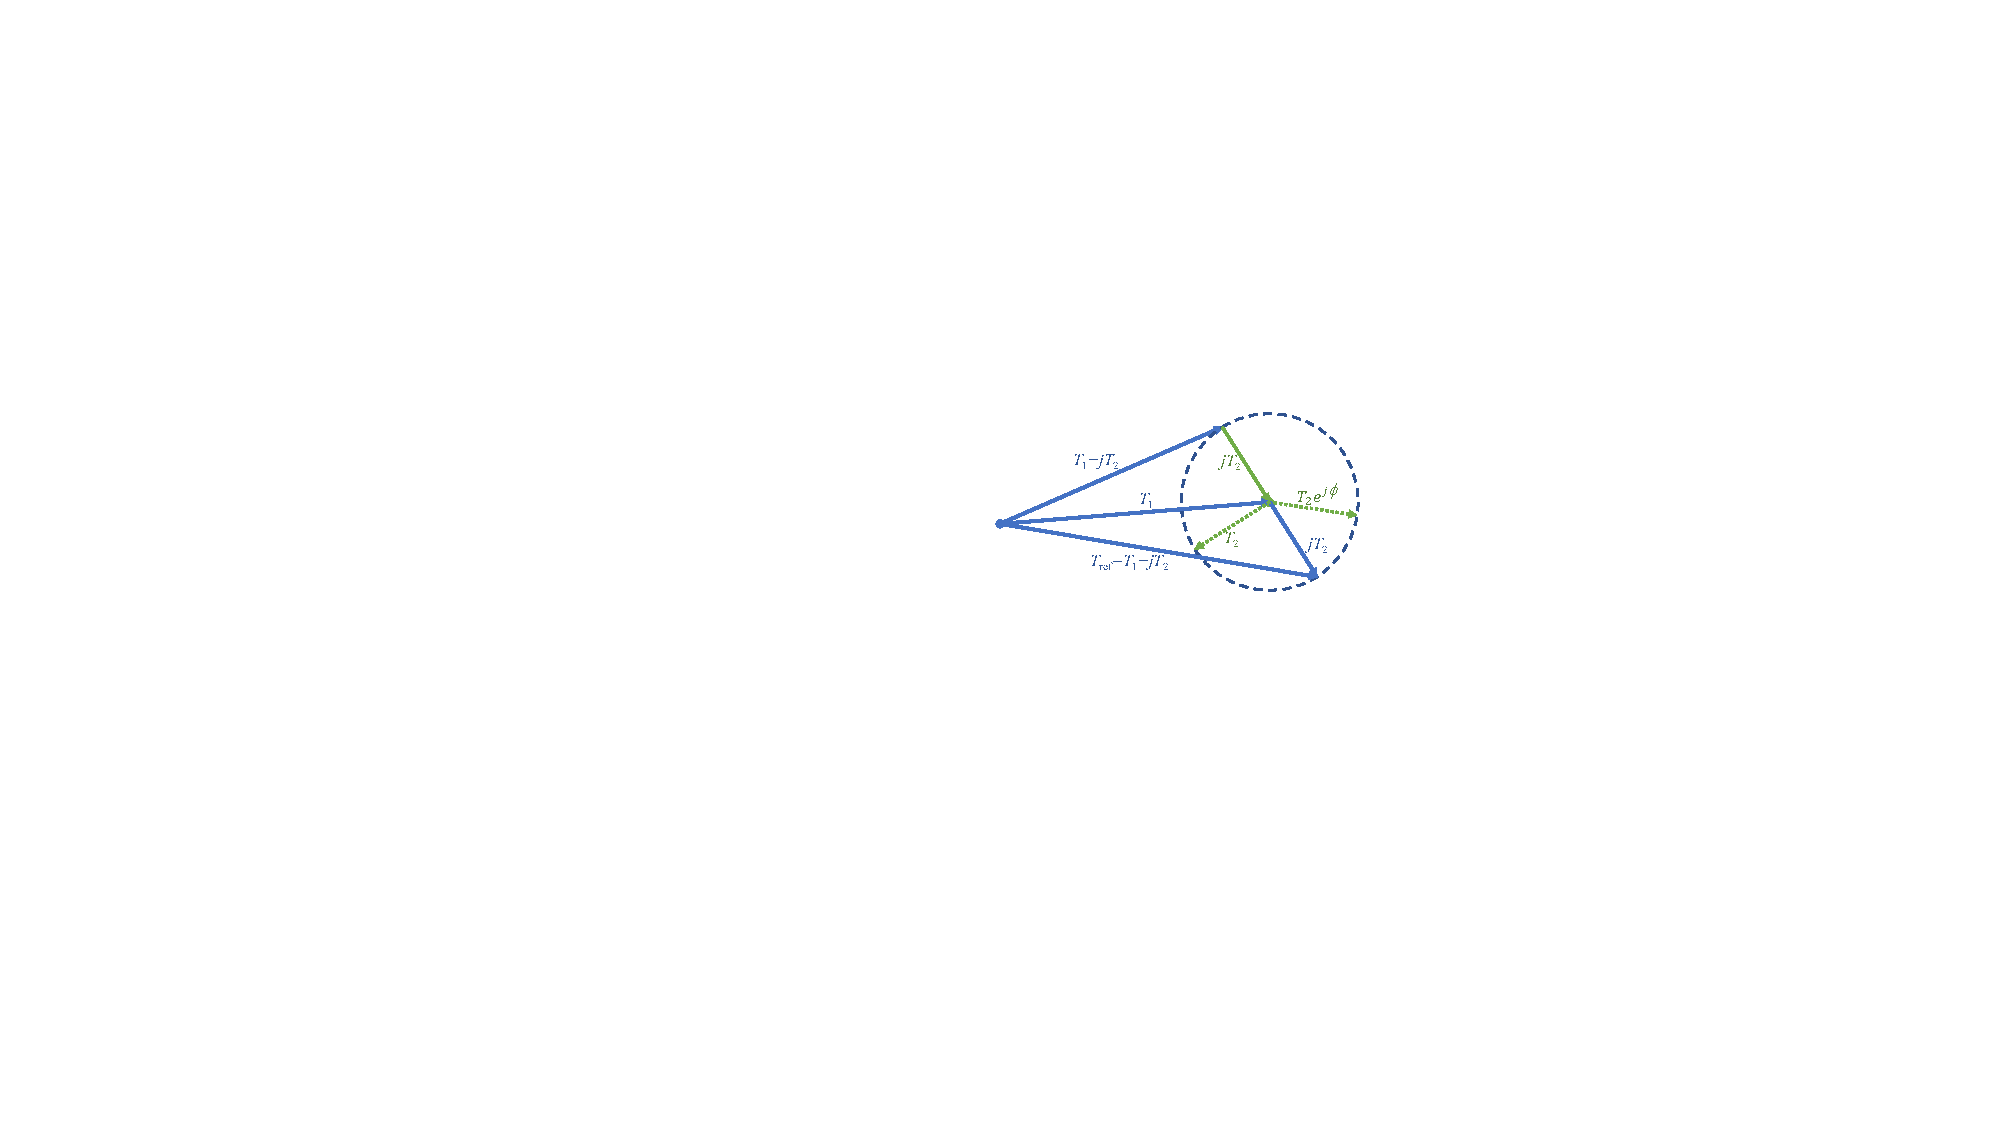
\includegraphics[width=0.5\linewidth]{cdma/cdma_phase_alignment}
	\caption{$T_1$、$T_2$与$T_{\text{ref}}$的几何关系图}
	\label{fig:cdma_phase_alignment}
\end{figure}

如图~\ref{fig:cdma_phase_alignment}所示，在RECD算法的单步优化中，目标相位$\psi = \arg(T_1 T_2^*)$旨在将当前单元信号 $T_2 e^{j\phi_{i,\lambda}}$ 对齐到背景矢量 $T_1$ 上。
然而，$T_1$ 的定义中包含了除当前单元外的其余单元贡献，在优化的过程中，$T_1$会随着目标单元的不同而变化。
若要实现非迭代求解，关键在于建立一个独立于当前单元状态的统一参考。观察式~\eqref{eq:cdma_phi_star}可以发现，最终的有效信道增益的方向与所有单元的相移为$\pi/2$时的方向是一致的。
定义所有单元相位均为 $\pi/2$ 时的全局参考信号为 $T_{\text{ref}} = j \sum_{l=1}^{N_e} u_{i,l}$，目标是求解当前单元信号$T_2$与$T_{\text{ref}}$的夹角$\psi_\lambda=\arg(T_{\text{ref}}T_2^*)$。
根据几何关系，有：
\begin{equation}\label{eq:cdma_TrefT2}
	T_{\text{ref}}T_2^* = (T_1+jT_2)T_2^*=T_1 T_2^* + j|T_2|^2.
\end{equation}
回顾式~\eqref{eq:cdma_linear_model}中的线性回归模型，有$T_1 T_2^*=\frac{1}{2}(x_1 + j x_2)$，代入上式并对其取模的平方，可得：
\begin{equation}
	|T_{\text{ref}}|^2|T_2|^2 =\frac{1}{4}(x_1^2+x_2^2)+x_2|T_2|^2+|T_2|^4,
\end{equation}
其中$|T_{\text{ref}}|^2 = |T_1+jT_2|^2=x_0+x_2-\sigma^2$，代入整理可得关于$|T_2|^2$的一元二次方程：
\begin{equation}
	|T_2|^4-(x_0-\sigma^2)|T_2|^2+\frac{1}{4}(x_1^2+x_2^2)=0.
\end{equation}

通常情况下，$|T_2|<|T_1|$，求解上述方程并取符合物理意义的较小正实根，有：
\begin{equation}
	|T_2|^2=\frac{x_0-\sigma^2-\sqrt{(x_0-\sigma^2)^2 - (x_1^2 + x_2^2)}}{2}.
\end{equation}
利用该能量值对观测矢量进行自干扰剔除，代入式~\eqref{eq:cdma_TrefT2}，可得：
\begin{equation}
	T_{\text{ref}}T_2^* =\frac{x_1}{2}+
	\frac{j\left( x_0+x_2-\sigma^2-\sqrt{(x_0-\sigma^2)^2 - (x_1^2 + x_2^2)}\right) }{2}.
\end{equation}
于是，当前单元信号$T_2$与$T_{\text{ref}}$的夹角可以估计为：
\begin{equation}\label{eq:cdma_hat_psi_lambda}
	\hat{\psi}_\lambda = \operatorname{atan2}\left(\hat x_0 +\hat x_2 - \sigma^2 - \sqrt{(\hat x_0 - \sigma^2)^2 - ( \hat x_1^2 +\hat x_2^2)},\; \hat x_1 \right).
\end{equation}
该解析式表明，最优相位配置完全由三个估计参数$(\hat x_0, \hat x_1, \hat x_2)$及噪声方差$\sigma^2$决定。基于上述推导，NI-REPA算法的执行流程如算法~\ref{alg:cdma_ni_repa}所示，执行一次算法的总测量次数为$T_{\text{meas}} = N_d \times N_e \times M$，这意味着在同等采样精度下，NI-REPA的导频开销仅为RECD算法的$1/K$，有效提升了波束赋形的配置效率。

\begin{algorithm}[!t]
	\caption{基于RSSI的非迭代逐元素相位对齐算法（NI-REPA）}
	\label{alg:cdma_ni_repa}
	\begin{algorithmic}[1]
		\REQUIRE 波导数量 $N_d$，单元数 $N_e$，采样点数 $M$，噪声方差 $\sigma^2$。
		\ENSURE 优化后的DMA配置矩阵$\bm{Q}$。
		\FOR{波导索引 $i = 1,\cdots,N_d$}
		\FOR{单元索引 $l = 1,\cdots,N_e$}
		\STATE 保持除 $l$ 外其余单元的相位为 $\pi/2$，依次设置 $\phi_{i,l} \in \{0, \frac{2\pi}{M}, \dots, \frac{2\pi(M-1)}{M}\}$，测量 $M$ 个接收功率值得到向量 $\bm p$；
		\STATE 根据式~\eqref{eq:cdma_hatbmx}计算中间参数 $\hat{x}_0, \hat{x}_1, \hat{x}_2$；
		\STATE 根据式~\eqref{eq:cdma_hat_psi_lambda}计算当前单元相对于全局参考的最优相位 $\hat{\psi}_l$；
		\ENDFOR
		\FOR{单元索引 $l = 1,\cdots,N_e$}
		\STATE 更新单元相位$\phi_{i,l} \leftarrow \hat{\psi}_l,\;[\bm Q]_{(i-1)N_e+l,i}\leftarrow (j+e^{j\phi_{i,l}})/2$；
		\ENDFOR
		\ENDFOR
		\RETURN DMA配置矩阵$\bm{Q}$。
	\end{algorithmic}
\end{algorithm}


\section{数值仿真分析}

\subsection{仿真参数设置}

本节将通过数值仿真验证所提的最优相位配置方法及基于RSSI的相位对齐算法的性能。考虑下行链路通信场景，基站配备的DMA阵列默认包含 $N_d = 10$ 条独立的微带波导，每条波导上集成 $N_e = 40$ 个辐射单元，总辐射单元数量为 $N = 400$。设定波导的衰减系数为 $\alpha = 0.5 \text{ Np/m}$，波数为 $\beta = 77.46 \text{ rad/m}$，相应的导波波长为 $\lambda_g = 2\pi/\beta$\cite{li2022digital}。为减小DMA单元间的互耦效应并满足弱耦合假设，辐射单元的间距设置为半个导波波长，即 $D = 0.5 \lambda_g$。
系统工作于典型的微波频段，载波频率设定为 $f_c = 2.6 \text{ GHz}$。基站的发射功率设定为 $P_t = 30 \text{ dBm}$，用户端的接收噪声功率为 $\sigma^2 = -100 \text{ dBm}$，基站与用户之间的距离为 $d = 100 \text{ m}$。大尺度衰落采用3GPP城市微小区路径损耗模型，其路损值计算公式为：
\begin{equation}
	\mathrm{PL} = 31.24 + 35.3 \log_{10}(d).
\end{equation}
除非在具体仿真中另有说明，本节所有的数值仿真均采用上述默认参数，且所有统计结果均通过 $N_{\mathrm{mc}} = 2000$ 次蒙特卡洛随机试验取平均得到。


\subsection{理论性能仿真与验证}

\begin{figure}[!htbp]
	\centering
	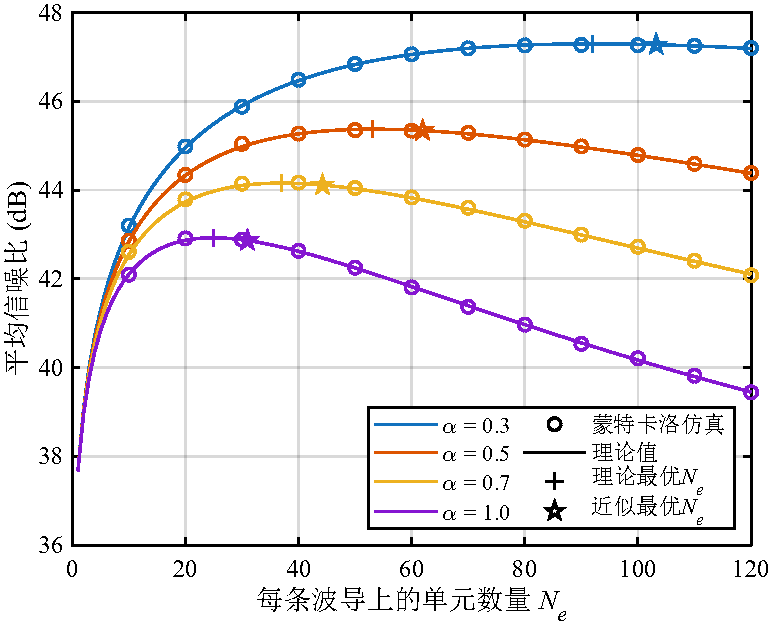
\includegraphics[width=0.6\linewidth]{cdma/cdma_figSNRvsNe.pdf}
	\caption{平均信噪比随单条波导辐射单元数量 $N_e$ 的变化趋势}
	\label{fig:cdma_figSNRvsNe}
\end{figure}

首先，图~\ref{fig:cdma_figSNRvsNe}展示了在不同波导衰减系数$\alpha$下，系统平均信噪比随单条波导上辐射单元数量$N_e$的变化关系。图中显示，对于所有的$\alpha$取值，仿真结果均与定理~\ref{the:cdma_gamma}给出的理论值完美吻合，验证了前文对平均信噪比推导的准确性。各条曲线的变化趋势验证了推论~\ref{cor:cdma_Ne_opt}中揭示的非单调特性：随着$N_e$的增加，平均信噪比呈现出先快速上升、达到峰值后缓慢下降的规律。
此外，图中还展示了波导衰减程度对系统性能及最佳阵列规模的影响。衰减系数$\alpha$越大，系统的最大平均信噪比越低，且达到峰值所需的单元数量也越少。图中分别标注了真实最优单元数量与根据式~\eqref{eq:cdma_Ne_opt}计算得到的近似最优数量。客观来看，随着 $\alpha$ 的增大，两者在横轴上出现了一定的偏差，近似公式给出的估计值略大于真实最优值。然而，从性能表现来看，由于曲线在峰值区域较为平缓，近似最优数量时的信噪比与全局最大信噪比之间的差距较小。这表明，近似公式依然能够作为一种快速的指导准则，帮助设计者根据衰减特性圈定最佳的天线规模区间，从而避免盲目增加天线单元带来的冗余与性能损失。


\begin{figure}[!htbp]
	\centering
	\begin{subfigure}[b]{0.48\linewidth}
		\centering
		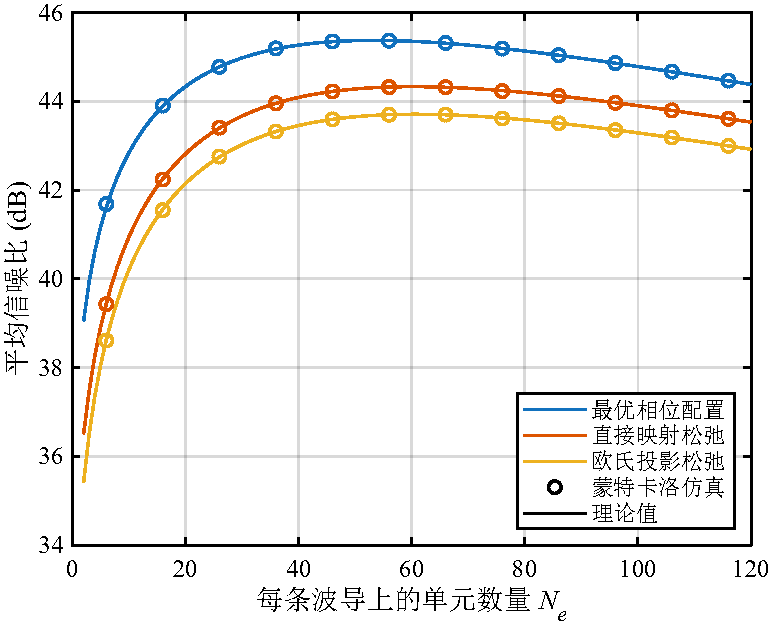
\includegraphics[height=5.8cm]{cdma/cdma_figSNRvsPhaseProjectionMethod.pdf}
		\caption{平均信噪比对比}
	\end{subfigure}%
	\hfill % 在两个子图之间水平填充空间
	\begin{subfigure}[b]{0.48\linewidth}
		\centering
		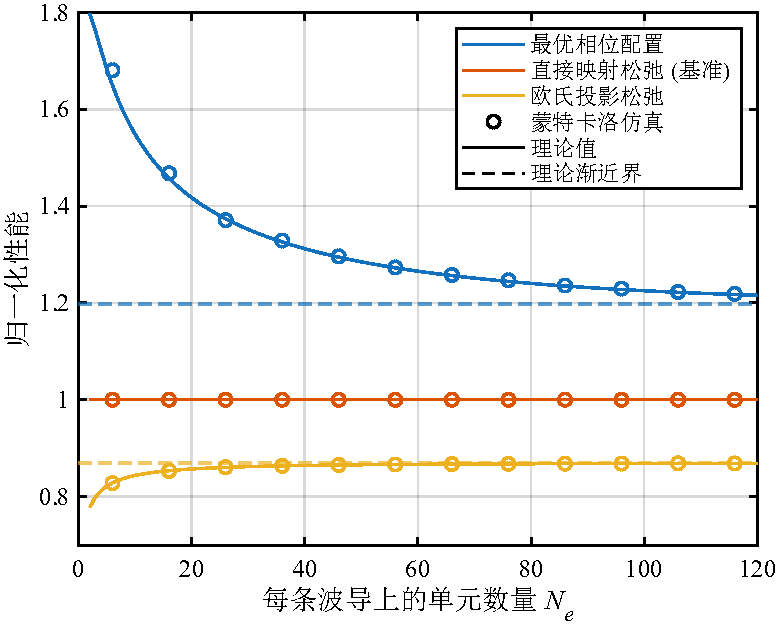
\includegraphics[height=5.8cm]{cdma/cdma_figNormalizedPhaseProjection.pdf}
		\caption{归一化渐近性能对比}
	\end{subfigure}
	\vspace{-0.5cm}
	\caption{三种相位配置方法的系统性能对比}
	\label{fig:cdma_phase_comparison}
\end{figure}

图~\ref{fig:cdma_phase_comparison}对比了所提的最优相位配置方法与现有研究中常用的直接映射松弛与欧氏投影松弛的性能表现。从图~\ref{fig:cdma_phase_comparison}(a)可以看出，两种松弛算法的仿真结果与推论~\ref{cor:cdma_gamma_relax}和推论~\ref{cor:cdma_gamma_proj}给出的理论曲线重合，并且三者均保持了随$N_e$先增后减的趋势。在绝对性能上，最优相位配置方法在整个$N_e$区间内均优于两种松弛方案，且直接映射松弛优于欧氏投影松弛，与前文的分析一致。为了验证前文的渐近性能分析，图~\ref{fig:cdma_phase_comparison}(b)以直接映射松弛的平均信噪比为基准，绘制了相应的归一化性能曲线。从图中可以看出，当每条波导上的辐射单元数量$N_e$较小时，最优方法带来的性能提升最为显著，相对增益可达 $70\%$ 左右。随着$N_e$的进一步增加，曲线逐渐趋于平缓。当$N_e$足够大时，最优相位配置与欧氏投影松弛的归一化性能精确地收敛于虚线所示的渐近界限，这与表~\ref{tab:cdma_comparison}中提取的渐近归一化性能一致。这表明，即使在大规模DMA阵列中，所提的最优相位配置方法相对于传统的松弛投影策略，依然能够保持一个恒定的性能优势。


\begin{figure}[!htbp]
	\centering
	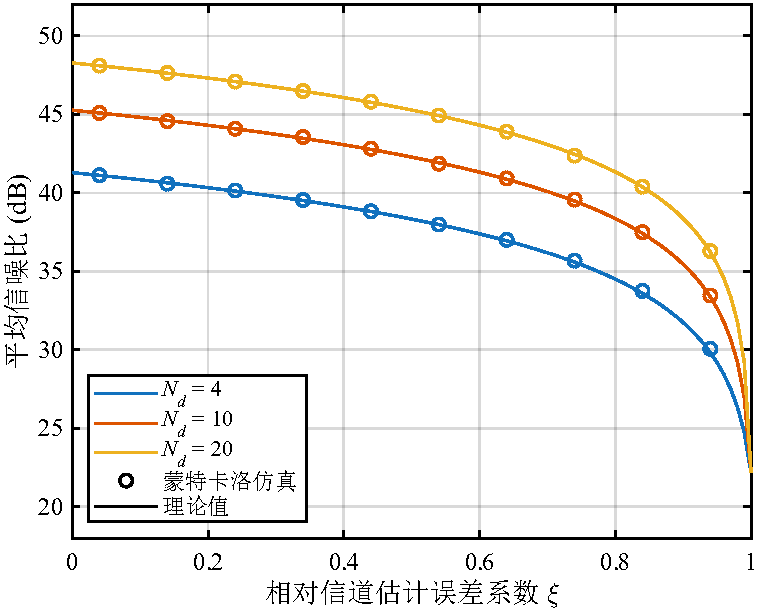
\includegraphics[width=0.6\linewidth]{cdma/cdma_figSNRvsImperfectCSI.pdf}
	\caption{平均信噪比随相对信道估计误差系数 $\xi$ 的变化趋势}
	\label{fig:cdma_figSNRvsImperfectCSI}
\end{figure}


图~\ref{fig:cdma_figSNRvsImperfectCSI}评估了非完美CSI对系统性能的影响，展示了平均信噪比随相对信道估计误差系数 $\xi$ 的变化曲线。从图中可以看出，在不同的波导数量 $N_d$ 配置下，仿真结果与推论~\ref{cor:cdma_gamma_imp}给出的理论曲线均吻合。随着误差系数 $\xi$ 的增大，由于信道估计的不准确导致相位发生严重失配，系统的平均信噪比呈现出显著的下降趋势。特别地，当信道估计完全失效时，不同波导数量对应的曲线最终收敛于同一个极低的信噪比水平，这一现象与前文的理论分析一致。另一方面，在相同的估计误差水平下，增加波导数量 $N_d$ 能够提升系统的整体信噪比。这表明，在信道获取质量受限的实际通信场景中，通过适度扩大基站端的DMA阵列规模，可以有效地弥补由于CSI不完美所带来的性能损失，从而保障系统传输的可靠性。

\begin{figure}[!htbp]
	\centering
	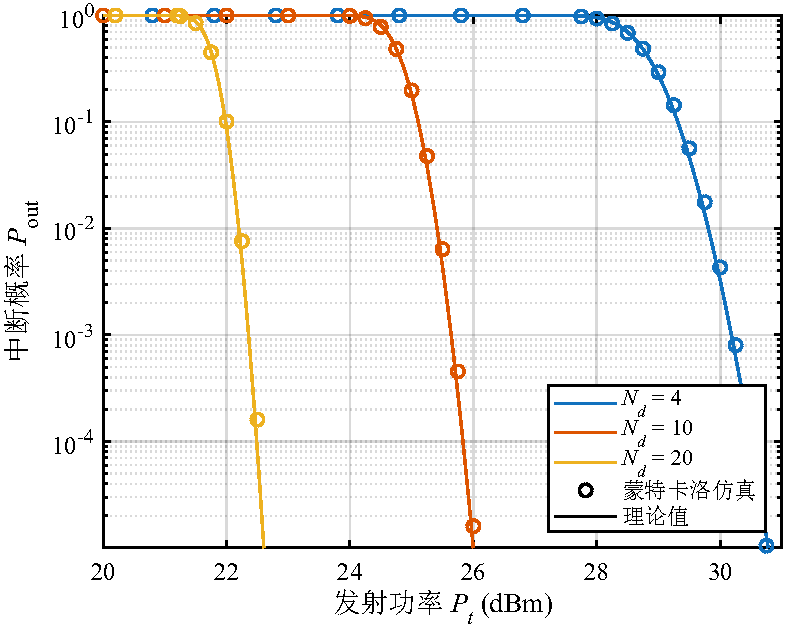
\includegraphics[width=0.6\linewidth]{cdma/cdma_figOutageProbabilityvsPt.pdf}
	\caption{系统中断概率随发射功率 $P_t$ 的变化曲线}
	\label{fig:cdma_figOutageProbabilityvsPt}
\end{figure}

为了更直观地评估DMA系统在最优相位配置下的通信可靠性，图~\ref{fig:cdma_figOutageProbabilityvsPt}展示了在不同波导数量配置下，中断概率随发射功率 $P_t$ 的变化关系，其中目标信噪比阈值设定为 $\gamma_{\text{th}} = 40 \text{ dB}$。从图中可以看出，基于伽马分布推导的中断概率理论曲线与蒙特卡洛仿真数据相吻合，说明对瞬时信噪比进行伽马分布建模是较为精确的。从性能趋势上看，所有配置下的曲线均呈现出典型的瀑布式下降特征。随着发射功率的提升，系统的中断概率呈指数级迅速降低。此外，随着 $N_d$ 从 $4$ 增加到 $20$，中断概率曲线大幅向左平移，表明增加波导数量能够提供更强的波束赋形增益，从而降低基站端的发射功率。


\begin{figure}[!htbp]
	\centering
	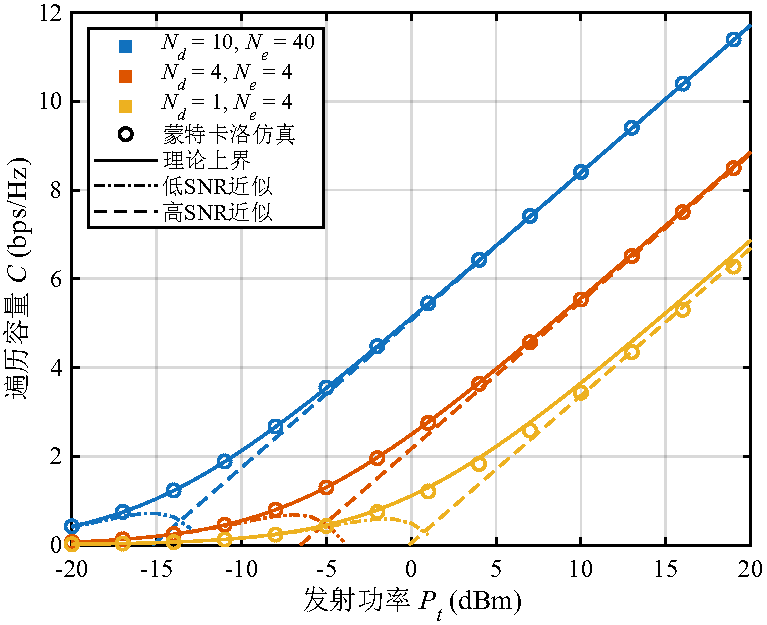
\includegraphics[width=0.6\linewidth]{cdma/cdma_figErgodicCapacity.pdf}
	\caption{系统遍历容量随发射功率 $P_t$ 的变化曲线}
	\label{fig:cdma_figErgodicCapacity}
\end{figure}

最后，图~\ref{fig:cdma_figErgodicCapacity}展示了在不同DMA阵列配置下，系统的遍历容量随基站发射功率 $P_t$ 的变化关系。图中同时绘制了蒙特卡洛仿真结果、式~\eqref{eq:cdma_capacity_upper}的理论上界，以及低信噪比和高信噪比条件下的渐近近似曲线。首先可以观察到，理论上界的紧致程度与DMA阵列的规模密切相关。对于黄色曲线所代表的小规模阵列，受瞬时信噪比起伏的影响，仿真值和理论上界有一定距离。然而，如前文分析所述，随着单元数量的增加，大量独立信道增益的叠加使得瞬时信噪比的波动变小，理论上界变得非常紧致。其次，两组渐近近似曲线也分别在各自的适用区间内表现出高度的准确性。在低发射功率区域，低SNR近似曲线有效追踪了容量的非线性增长；而在高发射功率区域，仿真点与高SNR近似曲线重合，验证了渐近推导的正确性。


\subsection{基于RSSI的相位对齐算法仿真分析}

\begin{figure}[!htbp]
	\centering
	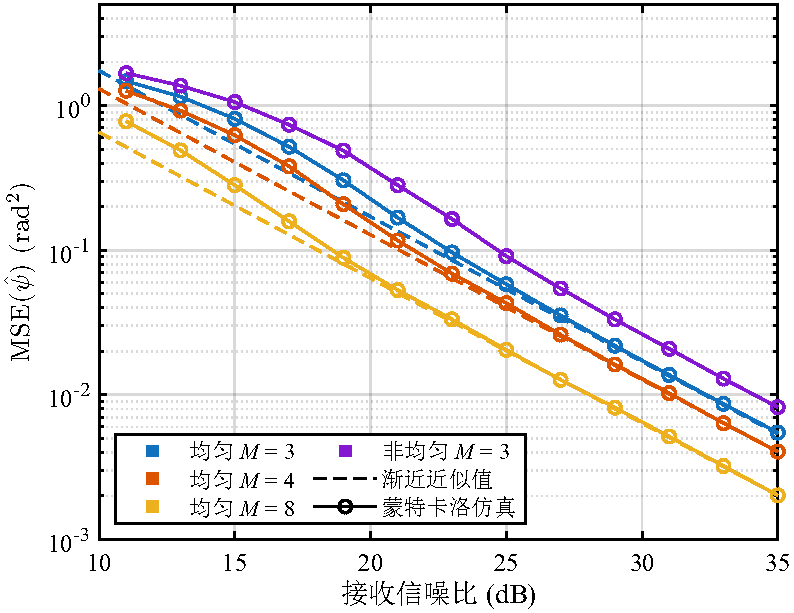
\includegraphics[width=0.6\linewidth]{cdma/cdma_figLinearEstimator.pdf}
	\caption{单个单元相位估计的均方误差随接收信噪比的变化曲线}
	\label{fig:cdma_figLinearEstimator}
\end{figure}

为了验证第~\ref{sec:cdma_phase_est_method}节中的相位估计理论，图~\ref{fig:cdma_figLinearEstimator}评估了相位估计量 $\hat{\psi}$ 的均方误差随接收信噪比的变化规律。从图中首先可以观察到，在较高信噪比区域，不同配置下的蒙特卡洛仿真曲线均与理论渐近近似虚线贴合，证明了线性回归误差分析模型的准确性。在采样策略的对比方面，当采样点数同为 $M=3$ 时，均匀采样策略的估计误差低于相位取值为 $\{0, \pi/2, \pi\}$ 的非均匀采样策略。这一结果印证了前文通过最小化信息矩阵逆的迹得出的理论结论，即均匀采样能最小化估计的MSE。此外，横向对比不同 $M$ 取值的均匀采样曲线可知，均方误差随着 $M$ 的增加呈比例下降。这表明在实际应用中，适当增加采样点数能提升相位估计的抗噪性能。

\begin{figure}[!htbp]
	\centering
	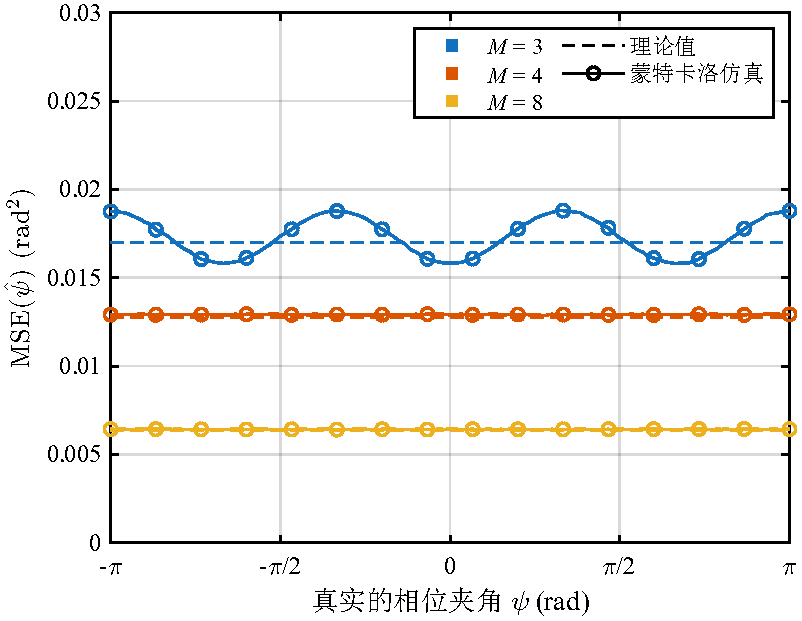
\includegraphics[width=0.6\linewidth]{cdma/cdma_figLinearEstimatorMSEvsPhase.pdf}
	\caption{单个单元相位估计的均方误差随真实相位夹角 $\psi$ 的变化曲线}
	\label{fig:cdma_figLinearEstimatorMSEvsPhase}
\end{figure}

在接收信噪比为 $30 \text{ dB}$ 的条件下，图~\ref{fig:cdma_figLinearEstimatorMSEvsPhase}展示了估计误差随 $T_1$ 和 $T_2$ 真实相位夹角 $\psi$ 的变化规律。当采样点数 $M \ge 4$ 时，仿真数据贴合理论水平线，表现出各向同性的特征；然而，当 $M=3$ 时，MSE呈现出随 $\psi$ 周期性波动的特征。其在 $[-\pi, \pi]$ 区间内包含三个完整的周期。这是因为在功率检测模型中，单次测量的观测噪声方差随相位夹角而波动，体现出异方差性。波动的方差项会通过三角函数乘积产生三倍频谐波项，导致 $M=3$ 时的估计方差受 $\psi$ 调制而发生波动。相比之下，当 $M \ge 4$ 时，高阶谐波项在对称均匀采样下抵消，使得估计方差呈现为与 $\psi$ 无关的水平直线。上述分析表明，尽管 $M=3$ 已满足最小参数求解自由度，但为确保在任意相位夹角下获得一致的估计精度，通常采样点数应至少设定为 $M=4$。

\begin{figure}[!htbp]
	\centering
	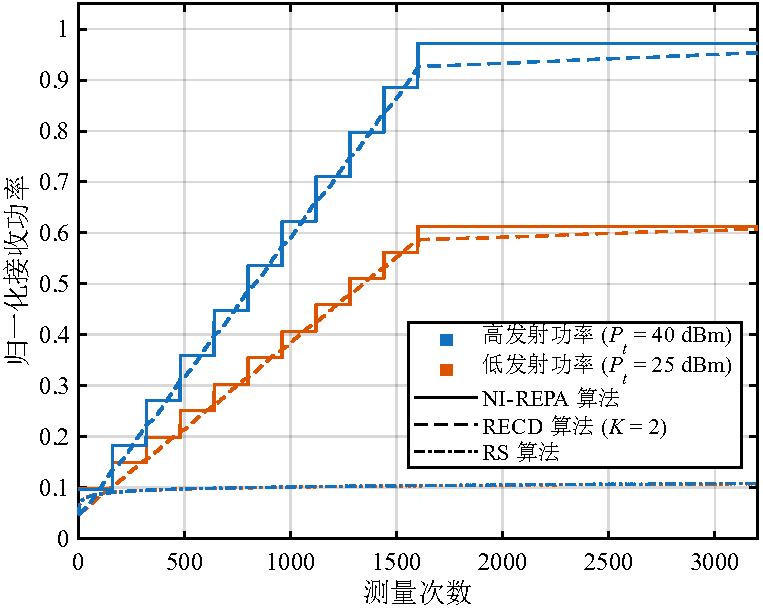
\includegraphics[width=0.6\linewidth]{cdma/cdma_figConvergence.pdf}
	\caption{不同算法的归一化接收功率随测量次数的收敛曲线}
	\label{fig:cdma_figConvergence}
\end{figure}

在采样点数 $M=4$ 的条件下，图~\ref{fig:cdma_figConvergence}展示了在高、低两种发射功率场景下，系统的归一化接收功率随测量次数的变化情况。其中，随机搜索算法为基准方案，完美CSI条件下的最优接收功率为归一化上限。从图中可以观察到，RS算法的收敛速度缓慢且性能低下。相比之下，本文提出的RECD算法和NI-REPA算法收敛速度较快。迭代两次的RECD算法表现为平滑的上升曲线；而NI-REPA算法由于采取集中测量、统一更新的方式，呈现出阶梯式跃升的特征。在高发射功率下，两种算法的归一化接收功率都达到了0.95以上，且NI-REPA算法的性能略优于RECD算法。这一结果表明，NI-REPA算法是一种高效的DMA阵列配置方案。

\begin{figure}[!htbp]
	\centering
	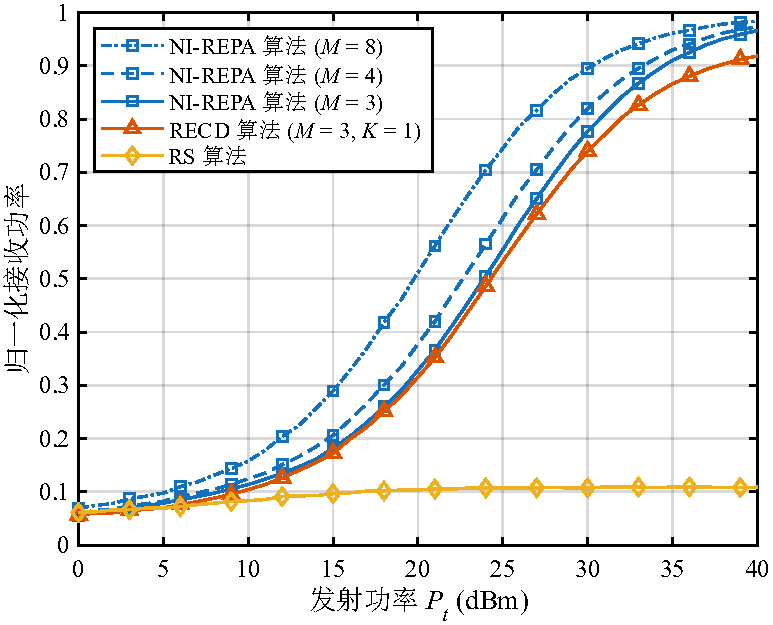
\includegraphics[width=0.6\linewidth]{cdma/cdma_figMNAPvsM.pdf}
	\caption{不同采样点数下算法归一化接收功率随发射功率 $P_t$ 的变化曲线}
	\label{fig:cdma_figMNAPvsM}
\end{figure}

最后，为了进一步探究采样点数 $M$ 对性能的影响，图~\ref{fig:cdma_figMNAPvsM}展示了不同配置下各个算法归一化接收功率随发射功率 $P_t$ 的变化规律。图中的曲线反映了所提算法在不同参数下的抗噪能力。随着 $P_t$ 增加，算法的相位估计误差减小，最终的归一化接收功率逐渐趋于理想情况。当发射功率达到 $40 \text{ dBm}$ 时，NI-REPA 算法的归一化接收功率超过 $0.95$，RECD 算法也突破了 $0.9$。此外，通过对比 $M=3,4,8$ 的曲线可知，增加采样点能改善低功率区域的性能，提高估计的鲁棒性。


\section{本章小结}




\noindent\rule{\linewidth}{2pt}


\noindent\rule{\linewidth}{2pt}

\chapter{离散相移DMA波束赋形性能分析与角域分划算法}\label{ch:ddma}


\section{引言}

\textcolor{red}{之后再写}

\section{系统模型}

本章继续研究基于DMA架构的下行链路单用户通信系统。基站天线阵列架构与第~\ref{sec:cdma_system_model}节保持一致，即包含$N_d$条平行微带波导，每条波导集成$N_e$个超材料辐射单元，共$N=N_d \times N_e$个单元。基站发射信号经数字预编码$\bm w$和DMA配置矩阵$\bm Q$处理后，通过信道$\bm g$传输至单天线用户。如图~\ref{fig:ddma_system}所示，与上一章假设相位连续可调的理想情况不同，本章将重点考察受硬件限制的实际应用场景，对DMA的相位离散特性及信道模型进行重新建模。

\begin{figure}[!htbp]
	\centering
	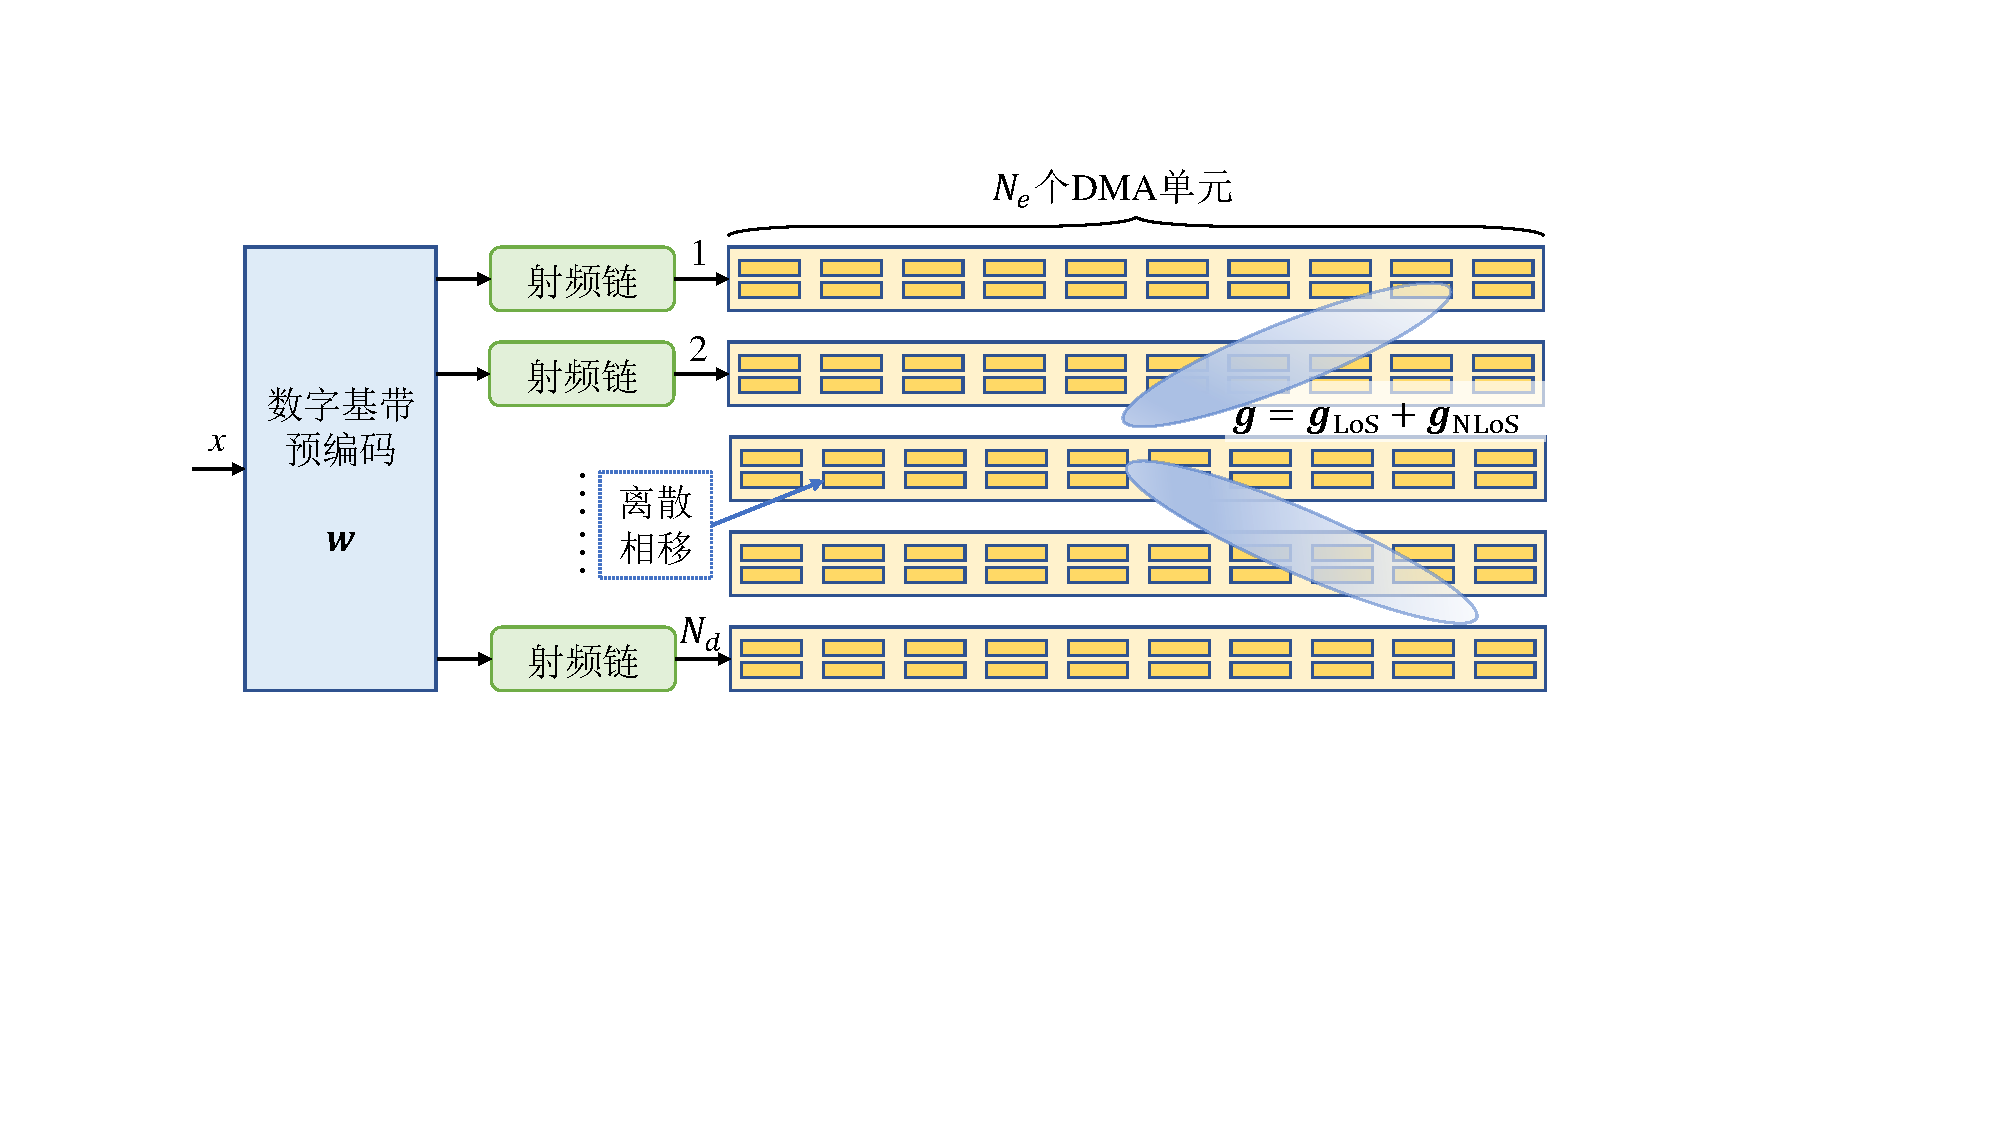
\includegraphics[width=0.7\linewidth]{ddma/ddma_system.pdf}
	\caption{离散相移DMA结构示意图}
	\label{fig:ddma_system}
\end{figure}

在实际的DMA硬件实现中，辐射单元的频率响应通常是通过加载变容二极管或PIN二极管等可调谐元件来控制的。
虽然变容二极管理论上支持连续调谐，但受限于数模转换器的精度，实际能够实现的相位状态是有限的。更常见的情况是采用PIN二极管，其仅具有“导通”和“截止”两种状态，只能提供低分辨率的相位控制。
图~\ref{fig:ddma_discrete_phase}展示了DMA在实际应用中面临的三种典型的离散相移特性：第一种为理想的均匀量化情形，其相位状态在$[0, 2\pi)$周期内均匀分布，常见于高精度数字控制的场景；第二种为非均匀离散相移情形，由于阵列面板制造公差或工作温度波动等原因，导致实际相位偏离均匀分布，呈现非均匀特性；第三种为移相能力受限情形，主要原因是受超材料单元极化率的谐振频率调控范围的物理限制，导致单元的调相范围无法覆盖完整的洛伦兹圆，只能在一定的角度范围内进行调节。

\begin{figure}[!htbp]
	\centering
	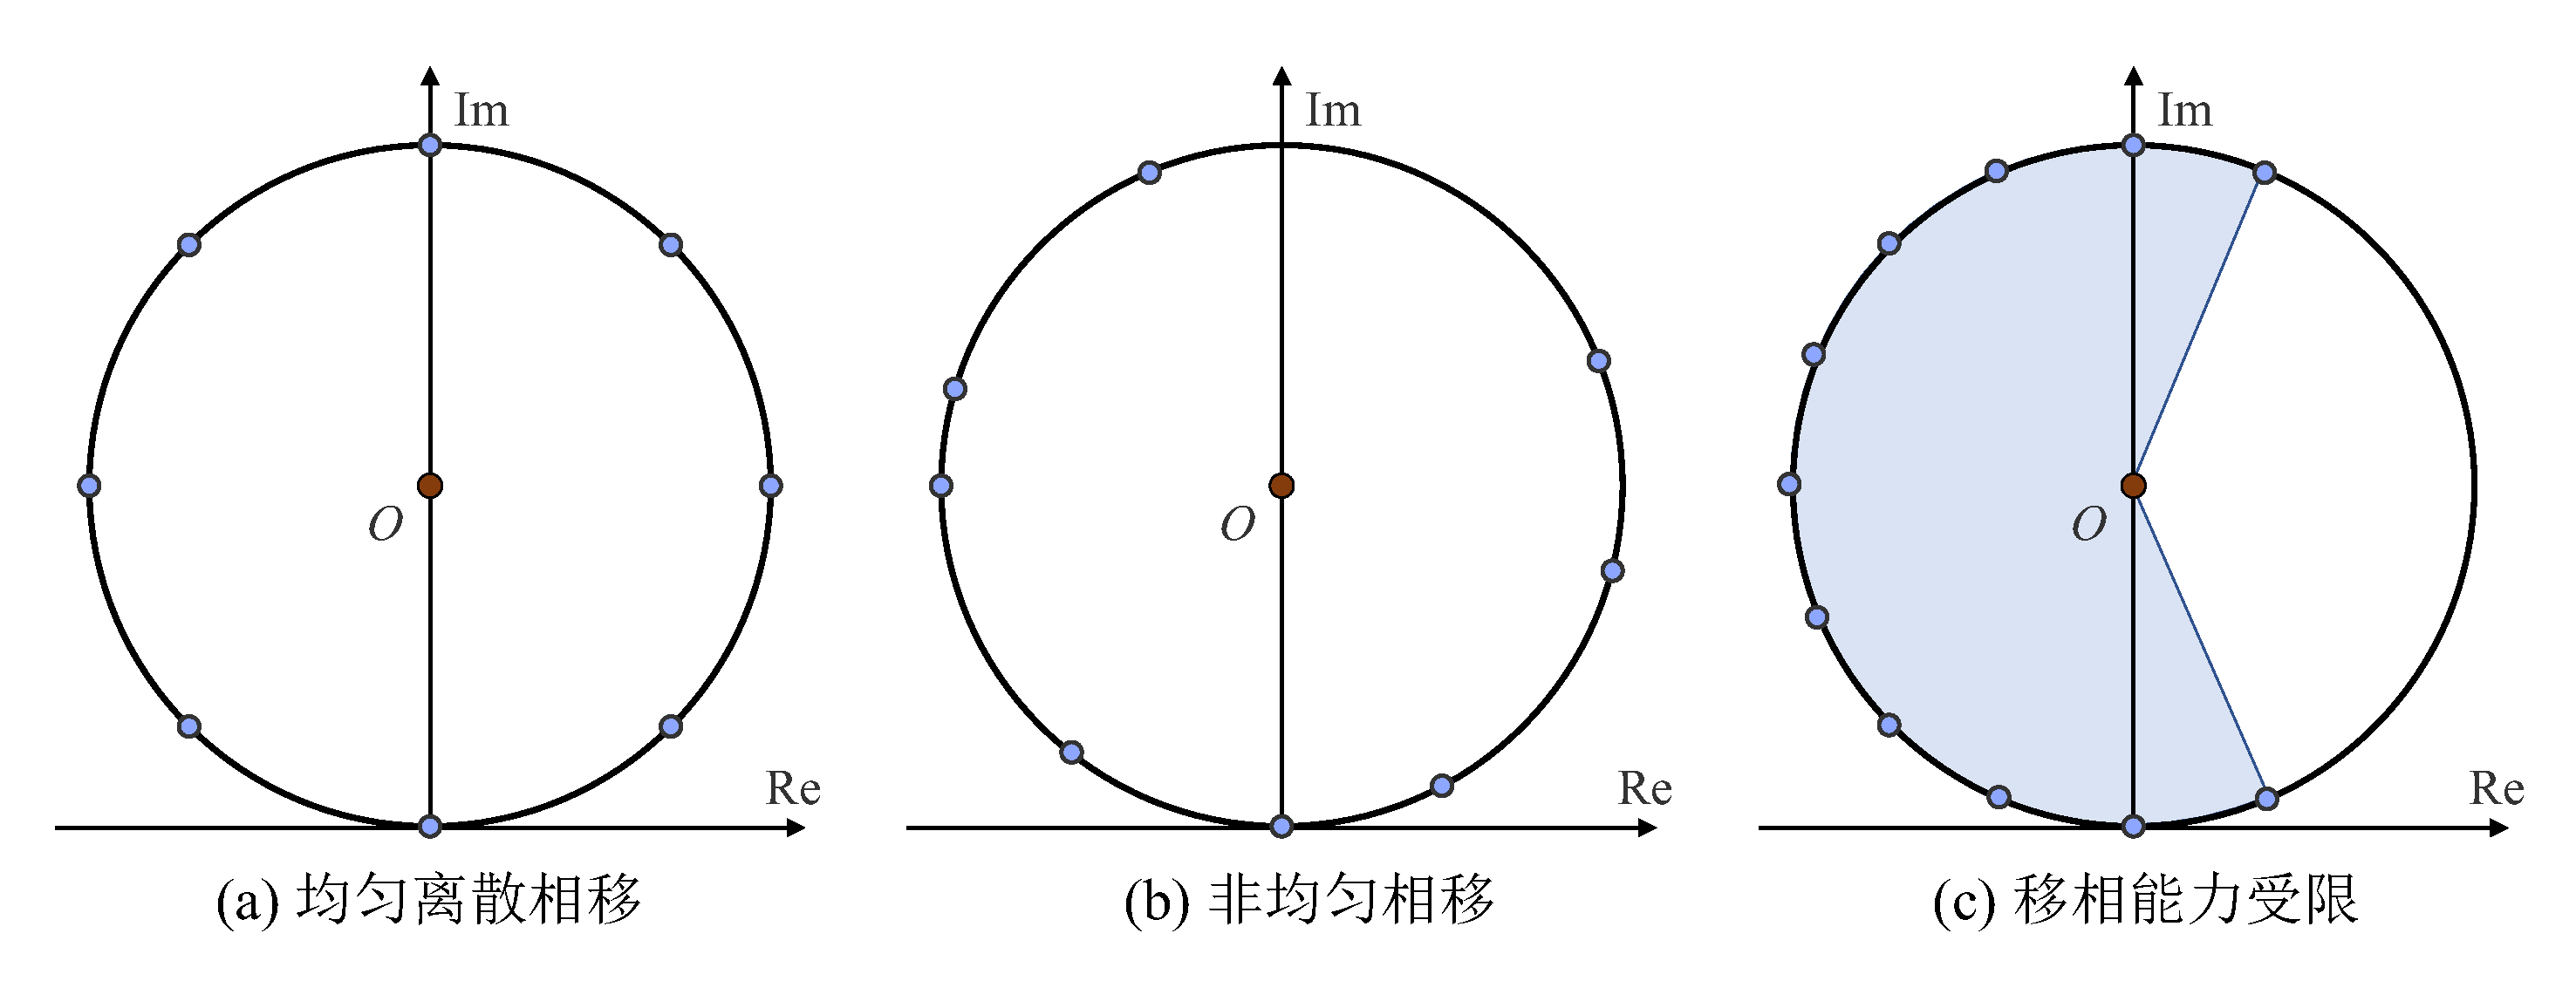
\includegraphics[width=0.8\linewidth]{ddma/ddma_discrete_phase.pdf}
	\caption{DMA实际相移特性的几种情况}
	\label{fig:ddma_discrete_phase}
\end{figure}

为了能够通用地分析上述各种离散特性，本章不再使用连续相位集合，而是将第$i$条波导上第$l$个单元的相位$\phi_{i,l}$建模为从一个有限的任意离散集合$\Phi_M$中取值：
\begin{equation}\label{eq:ddma_discrete_set}
	\phi_{i,l} \in \bm \Phi_M = \{\Phi_1, \Phi_2, \cdots, \Phi_M\}, \quad \forall i, l,
\end{equation}
其中$M$表示可取的相位状态数量。不失一般性，假设离散相位值满足如下关系：
\begin{equation}
	0 \le \Phi_1 < \Phi_2 < \cdots < \Phi_M < 2\pi.
\end{equation}
在此基础上，定义移相能力$C=\Phi_M-\Phi_1$，对于移相能力受限的情形，满足$C<\frac{2\pi(M-1)}{M}$，这意味着此时$M$个离散相位点无法在$[0, 2\pi)$周期内实现均匀分布。
相应地，DMA单元的权重系数仍满足式~\eqref{eq:cdma_qil}的洛伦兹形式耦合关系，但相位受到式~\eqref{eq:ddma_discrete_set}的严格约束。

在上一章中，研究假设了瑞利衰落信道。然而，DMA通常应用于视距分量较强的场景，且由于DMA与用户之间的距离远大于DMA自身的物理尺寸，各单元到用户的路径损耗可近似认为相同。
因此，本章采用莱斯衰落模型来描述DMA阵列与用户之间的信道$\bm g \in \mathbb{C}^{N \times 1}$：
\begin{equation}\label{eq:ddma_rician_channel}
	\bm g = \sqrt{\rho} \left( \sqrt{\frac{\kappa}{\kappa+1}}\bar{\bm g} + \sqrt{\frac{1}{\kappa+1}}\tilde{\bm g} \right),
\end{equation}
其中，$\rho$表示距离相关的路径损耗；$\kappa$为莱斯因子，表征视距分量与非视距分量的功率比；$\bar{\bm g}$和$\tilde{\bm g}$分别表示确定的视距分量和随机的非视距散射分量。

基于上述模型，为了最大化用户端的接收信噪比，需对DMA的权重矩阵$\bm Q$进行优化。最优的数字预编码向量$\bm w$仍然采用最大比传输策略获得，此时的离散优化问题为：
\begin{equation}\label{eq:ddma_pQ}
	\max_{\bm{Q}} \quad  p(\bm{Q})=\|\bm{g}^\mathrm{T} \bm{HQ}\|^2,
	\quad \text{s.t.} \quad  \eqref{eq:cdma_Q}, \;
	\eqref{eq:ddma_discrete_set}.
\end{equation}
该优化问题属于典型的非凸整数非线性规划问题。若采用穷举法寻找全局最优解，搜索空间高达$\mathcal{O}(M^{N_d N_e})$，对于大规模DMA阵列而言，指数级增长的计算复杂度在实际中不可行。
为了在性能与计算复杂度之间取得平衡，下文将提出一种基于最近点投影的低复杂度次优算法。

\section{最近点投影算法与离散性能分析}

本节首先针对任意离散相移场景介绍最近点投影算法，随后，基于前述信道模型推导系统平均信噪比的闭式解，并以此为基础全面分析DMA离散相移分布特性对系统性能的影响。

\subsection{任意离散相移的最近点投影算法}

针对离散相移约束，一种直观且高效的求解思路是首先忽略离散约束，获取连续相移条件下的最优解（如第\ref{ch:cdma}章定理~\ref{the:cdma_Qstar}所述），随后，在离散相位集合$\bm \Phi_M$中寻找与连续最优解相位差最小的离散点作为最终解。
这种方法的理论依据在于，随着离散相移选择$M$的数量增加，离散问题的解空间将逐渐逼近连续情形\cite{you2020channel, wang2021dynamic, abeywickrama2020intelligent}。
具体来说，对于连续最优相位$\phi_{i,l}^\star$，其对应的离散解$\phi_{i,l}^{\text{CPP}}$可通过下式获得：
\begin{equation}
	\phi_{i,l}^{\text{CPP}} = \mathop{\arg\max}_{\phi \in \bm \Phi_M} \cos(\phi_{i,l}^\star-\phi).
\end{equation}

尽管CPP算法获得的解$\bm Q^{\text{CPP}}$可能不是优化问题~\eqref{eq:ddma_pQ}的全局最优解，但该方法避免了处理非凸约束所需的复杂迭代过程。
在计算复杂度方面，CPP算法仅需对每个单元的连续最优相位在$M$个离散值中进行一次最近邻搜索，其总计算复杂度降低为$\mathcal{O}(MN_dN_e)$。
该算法的具体执行步骤总结于算法~\ref{alg:ddma_cpp}中。

\begin{algorithm}[!t]
	\caption{离散相移最近点投影算法（CPP）}
	\label{alg:ddma_cpp}
	\begin{algorithmic}[1]
		\REQUIRE 信道向量$\bm g$，波导传输矩阵$\bm H$，波导数$N_d$，单元数$N_e$，量化相移数$M$，离散相位集$\bm \Phi_M$。
		\ENSURE 离散相移DMA配置矩阵$\bm Q^{\text{CPP}}$。
		\STATE 初始化配置矩阵 $\bm Q^{\text{CPP}}=\bm 0_{N\times N_d}$；
		\FOR {$i=1,2,\cdots, N_d$}
		\FOR {$l=1,2,\cdots, N_e$}
		\STATE 根据第\ref{ch:cdma}章定理~\ref{the:cdma_Qstar}计算连续最优相位 $\phi_{i,l}^\star$；
		\FOR {$m=1,2,\cdots, M$}
		\STATE 计算投影相关系数 $A_m=\cos(\phi_{i,l}^\star-\Phi_m)$；
		\ENDFOR
		\STATE 选取相关系数最大的索引 $m^\star=\mathop{\arg\max}\limits_{1\leq m \leq M} (A_m)$；
		\STATE 确定离散相位 $\hat{\phi}_{i,l}\leftarrow\Phi_{m^\star}$，更新配置矩阵 $[\bm Q^{\text{CPP}}]_{(i-1)N_e+l, i} = (j+e^{j \phi_{i,l}^{\text{CPP}}})/2$；
		\ENDFOR
		\ENDFOR
		\RETURN $\bm Q^{\text{CPP}}$。
	\end{algorithmic}
\end{algorithm}

\subsection{任意离散相移下的平均信噪比分析}

本小节将推导任意离散相移约束下，采用CPP算法时DMA系统的平均信噪比闭式解。根据式~\eqref{eq:cdma_gamma}定义的平均信噪比，代入式~\eqref{eq:ddma_rician_channel}中的莱斯衰落信道模型，并应用CPP算法得到的离散权重系数$\bm Q^{\text{CPP}}$，由于所有波导具有相同的统计特性，平均信噪比 $\gamma^{\text{CPP}}$ 可展开为：
\begin{equation}\label{eq:ddma_gamma_expand}
	\gamma^{\text{CPP}} = \frac{P_t \rho N_d}{\sigma^2} \left( \frac{\kappa}{\kappa+1} \mathbb{E}_{\text{LoS}} + \frac{1}{\kappa+1} \mathbb{E}_{\text{NLoS}} \right),
\end{equation}
其中 $\mathbb{E}_{\text{LoS}}$ 和 $\mathbb{E}_{\text{NLoS}}$ 分别表示第$i$条波导的视距分量和非视距分量对应的归一化期望增益：
\begin{equation}
	\mathbb{E}_{\text{LoS}} = \mathbb{E}\left(\left| \sum_{l=1}^{N_{e}} \bar{g}_{i,l} h_{i, l} q_{i,l}^{\text{CPP}}\right|^{2}\right), 
	\quad
	\mathbb{E}_{\text{NLoS}} = \mathbb{E}\left(\left| \sum_{l=1}^{N_{e}} \tilde{g}_{l} h_{i, l} q_{i,l}^{\text{CPP}}\right|^{2}\right).
\end{equation}

首先分析视距分量$\mathbb{E}_{\text{LoS}}$。定义CPP算法引入的量化相位误差为 $\varphi_{i,l} = \phi_{i,l}^{\text{CPP}} - \phi_{i,l}^\star$。
将 $q_{i,l}^{\text{CPP}} = (j+e^{j(\phi_{i,l}^\star + \varphi_{i,l})})/2$ 以及连续最优相位 $\phi_{i,l}^\star$ 的表达式代入，并利用 $\bar{g}_{i,l}$ 的单位模性质，$\mathbb{E}_{\text{LoS}}$ 可化简为：
\begin{equation}\label{eq:ddma_ELoS_def}
	\mathbb{E}_{\text{LoS}} = \frac{1}{4} \mathbb{E}\left( \left| |\Lambda_i| + \sum_{l=1}^{N_e} |\bar{g}_{i,l} h_{i,l}| e^{j\varphi_{i,l}} \right|^2 \right),
\end{equation}
其中 $\Lambda_i = j \sum_{l=1}^{N_{e}} \bar{g}_{i,l} h_{i,l}$ 为与量化误差无关的常数项。对模平方进行展开，得到如下三项之和：
\begin{equation}\label{eq:ddma_ELoS_terms}
	\medmath{
		\mathbb{E}_{\text{LoS}} = \frac{1}{4} \mathbb{E}
		\bigg( \underbrace{|\Lambda_i|^2 + \sum_{l=1}^{N_e} |\bar{g}_{i,l} h_{i,l}|^2}_{A_1} + \underbrace{2|\Lambda_i| \sum_{l=1}^{N_e} |\bar{g}_{i,l} h_{i,l}| \cos \varphi_{i,l}}_{A_2} + \underbrace{\sum_{l \ne \lambda} |\bar{g}_{i,l} h_{i,l}| |\bar{g}_{i,\lambda} h_{i,\lambda}| e^{j(\varphi_{i,l} - \varphi_{i,\lambda})}}_{A_3} \bigg).
	}
\end{equation}

下面逐项计算 $A_1, A_2, A_3$ 的期望值。
首先将$\mathbb{E}(A_1)$表达为自相关项与互相关项之和：
\begin{equation}\label{eq:ddma_EA1_expand}
	\mathbb{E}(A_1) = \mathbb{E}\left( 2\sum_{l=1}^{N_e} |\bar{g}_{i,l} h_{i,l}|^2 + \sum_{l=1}^{N_e} \sum_{\substack{\lambda=1 \ \lambda \neq l}}^{N_e} \bar{g}_{i,l} h_{i,l} \bar{g}_{i,\lambda}^* h_{i,\lambda}^* \right).
\end{equation}
由于视距分量 $\bar{g}_{i,l}$ 具有单位模，且假设其相位在 $[0, 2\pi)$ 内服从独立均匀分布 ，则交叉项的期望满足：
\begin{equation}
	\mathbb{E}(\bar{g}_{i,l} h_{i,l} \bar{g}_{i,\lambda}^* h_{i,\lambda}^*) =
	\begin{cases}
		|h_{i,l}|^2, & \text{若}\; l=\lambda, \\
		0, & \text{否则}.
	\end{cases}
\end{equation}
因此，式~\eqref{eq:ddma_EA1_expand}中的第二项求和结果为零。结合波导衰减模型 $|h_{i,l}| = e^{-\alpha D(l-1)}/\sqrt{N_e}$，可得：
\begin{equation}
	\mathbb{E}(A_1) = 2 \sum_{l=1}^{N_e} |h_{i,l}|^2 = \frac{2}{N_e} \frac{1 - e^{-2\alpha D N_e}}{1 - e^{-2\alpha D}}.
\end{equation}

对于项 $A_2$，当单元数量 $N_e > 2$ 时，可以合理假设 $\Lambda_i$、信道项$\bar{g}_{i,l} h_{i,l}$与量化误差 $\varphi_{i,l}$ 之间相互独立。
当$N_e$较大时，根据中心极限定理，$\Lambda_i$近似服从循环对称复高斯分布，相应地，其模值$|\Lambda_i|$近似服从瑞利分布，其均值为：
\begin{equation}
	\mathbb{E}(|\Lambda_i|) = \frac{\sqrt{\pi}}{2} \sqrt{\sum_{l=1}^{N_e} |h_{i,l}|^2} = \frac{\sqrt{\pi}}{2\sqrt{N_e}} \sqrt{\frac{1 - e^{-2\alpha D N_e}}{1 - e^{-2\alpha D}}}.
\end{equation}
将上述期望代入 $A_2$ 的定义式，其期望取决于量化误差的余弦期望 $\mathbb{E}(\cos \varphi_{i,l})$，即：
\begin{equation}
	\mathbb{E}(A_2) = \frac{\sqrt{\pi}}{N_e} \sqrt{\frac{1 - e^{-2\alpha D N_e}}{1 - e^{-2\alpha D}}} \frac{1 - e^{-\alpha D N_e}}{1 - e^{-\alpha D}} \mathbb{E}(\cos \varphi_{i,l}).
\end{equation}

最后计算项$A_3$的期望，由于不同单元的量化误差 $\varphi_{i,l}$ 和 $\varphi_{i,\lambda}$ 相互独立，且 $\mathbb{E}(e^{j\varphi_{i,l}}) = \mathbb{E}(\cos \varphi_{i,l})$，有：
\begin{equation}
	\mathbb{E}(A_3) = \frac{1}{N_e} \left[ \left(\frac{1 - e^{-\alpha D N_e}}{1 - e^{-\alpha D}}\right)^2 - \frac{1 - e^{-2\alpha D N_e}}{1 - e^{-2\alpha D}} \right]\cdot [\mathbb{E}(\cos \varphi_{i,l})]^2.
\end{equation}

\begin{figure}[!htbp]
	\centering
	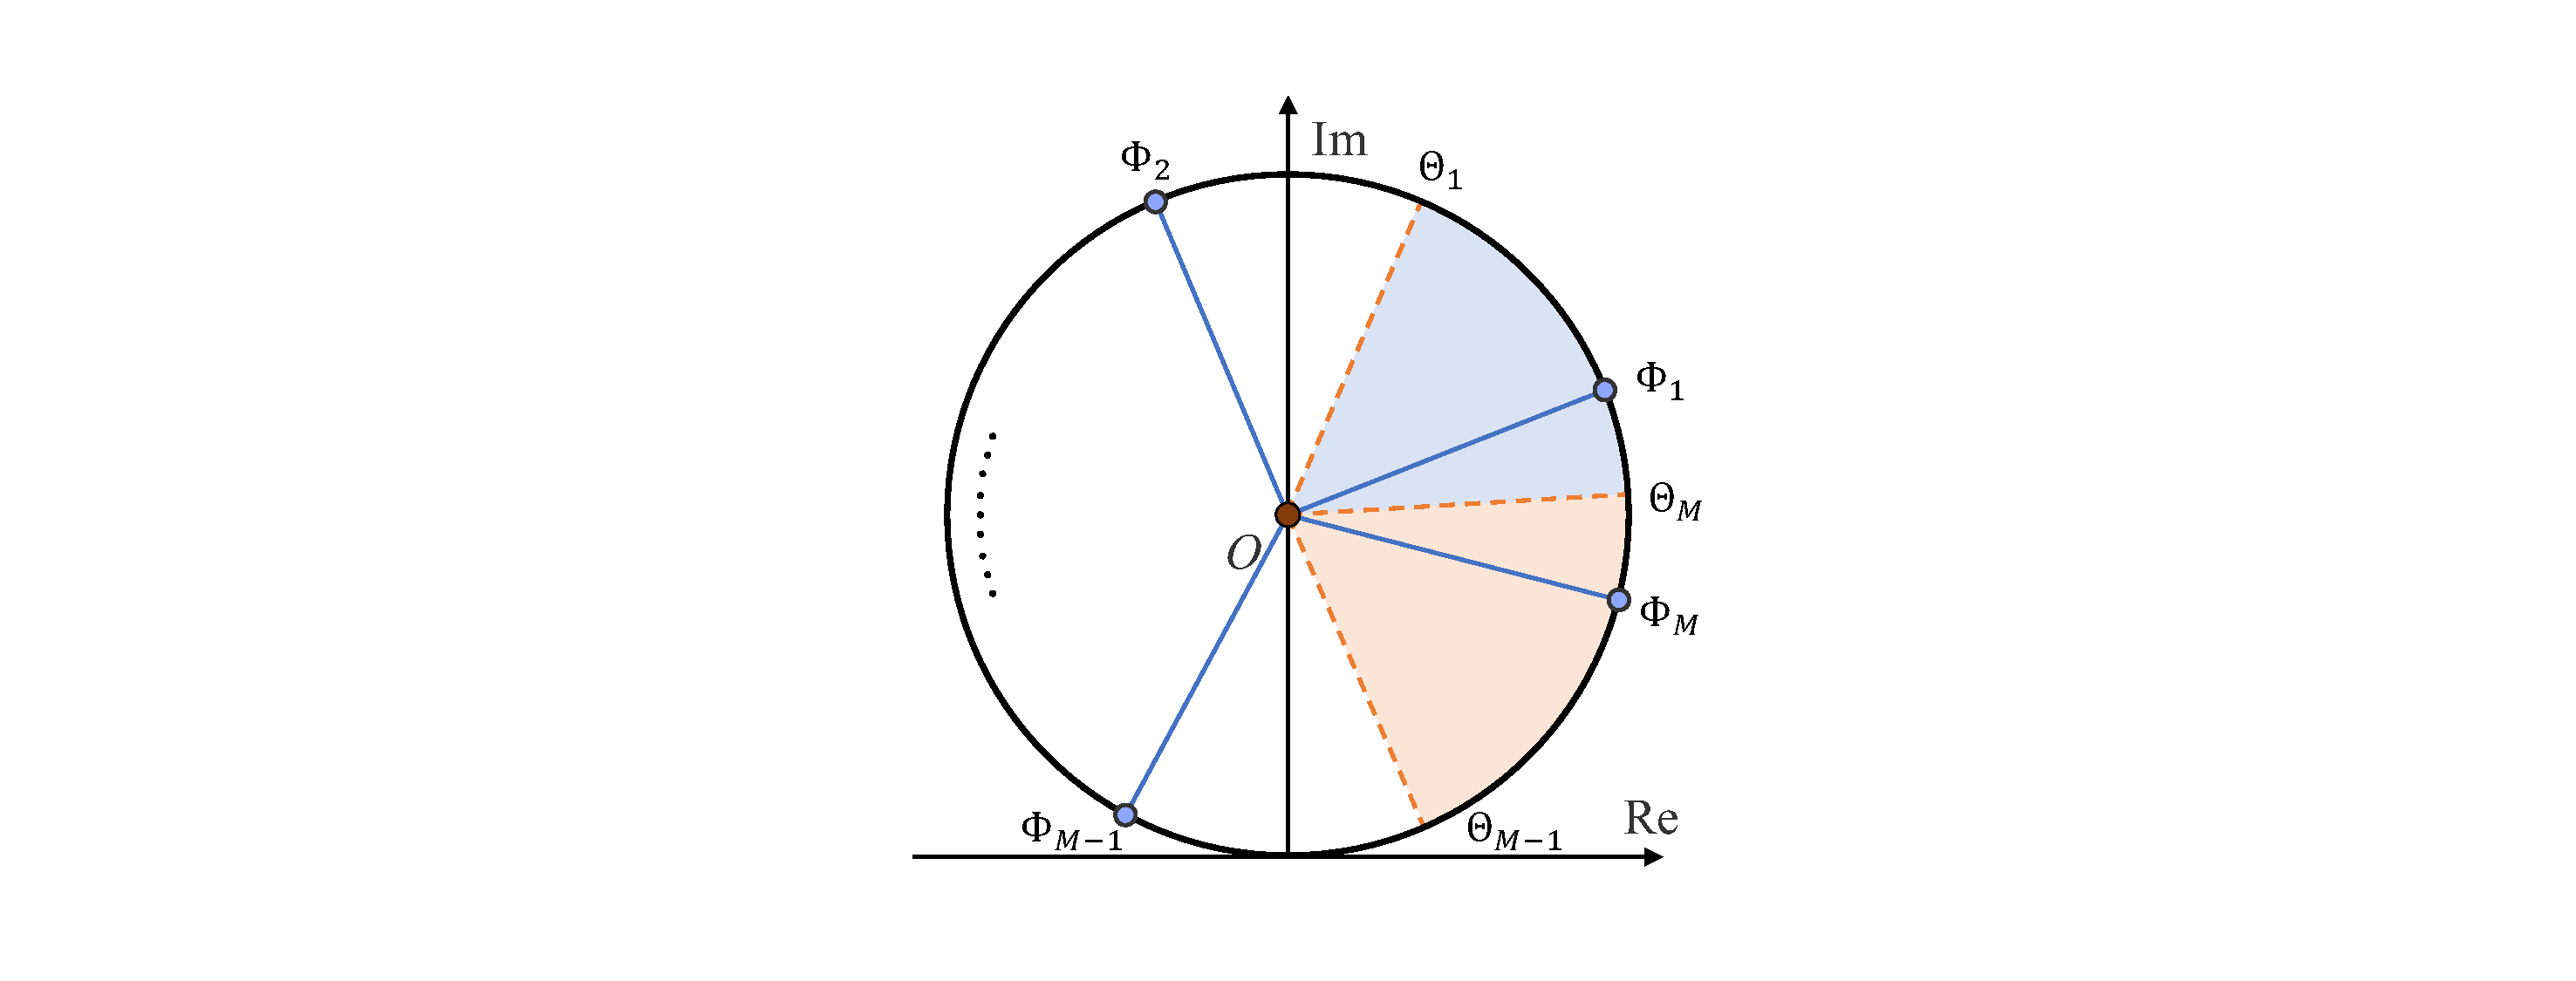
\includegraphics[width=0.4\linewidth]{ddma/ddma_cos.pdf}
	\caption{CPP算法的相位量化区间与决策边界}
	\label{fig:ddma_cos}
\end{figure}

上述推导中的关键在于量化误差的统计特性。
如图~\ref{fig:ddma_cos}所示，在洛伦兹圆上对量化误差进行分区讨论。
由于连续最优相位 $\phi_{i,l}^\star$ 在 $[0, 2\pi)$ 上均匀分布，其概率密度函数为 $f(\phi) = \frac{1}{2\pi}$。
图中蓝色实心点表示离散相位集合 $\bm \Phi_M$，橙色虚线表示相邻离散相位之间的决策边界 $\Theta_m$。
根据最近点投影原则，决策边界位于相邻两点的角平分线上，即：$\Theta_m=\frac{\Phi_m+\Phi_{m+1}}{2}$。
对于最终量化为$\Phi_m$的连续解而言，其量化误差在$[\Theta_{m-1}-\Phi_m,\Theta_{m}-\Phi_m]$上均匀分布。
为了计算全周期的期望值 $\mathbb{E}(\cos \varphi_{i,l})$，将整个 $[0, 2\pi)$ 积分域分解为 $M$ 个这样的子区间之和，有：
\begin{align}
	\mathbb{E}(\cos \varphi_{i,l}) 
	&= \int_{0}^{2\pi} \frac{1}{2\pi}\cos(\phi^{\text{CPP}} - \phi) \, \mathrm{d}\phi \\
	&= \sum_{m=1}^M \left( \int_{-\frac{\Phi_{m}-\Phi_{m-1}}{2}}^{\frac{\Phi_{m+1}-\Phi_m}{2}} \frac{1}{2\pi} \cos \varphi \, \mathrm{d}\varphi \right) \\
	&= \frac{1}{2\pi} \sum_{m=1}^M
	\left( \sin\left(\frac{\Phi_{m+1}-\Phi_m}{2}\right)
	+ \sin\left(\frac{\Phi_{m}-\Phi_{m-1}}{2}\right)
	\right) \\
	&= \frac{1}{\pi} \sum_{m=1}^M \sin \frac{\Phi_{m+1}-\Phi_m}{2},\label{eq:ddma_E_cos_phi}
\end{align}
其中约定 $\Phi_{M+1} = \Phi_1 + 2\pi$ 以处理循环边界条件。

类似地，对于非视距分量，由于信道 $\tilde{g}_{i,l}$ 的随机性占主导，离散相位的具体取值对平均功率的影响被平均化，可推导得：
\begin{equation}
	\mathbb{E}_{\text{NLoS}} = \frac{1}{2N_e} \frac{1 - e^{-2\alpha D N_e}}{1 - e^{-2\alpha D}}.
\end{equation}
综合上述各项结果，并代入式~\eqref{eq:ddma_gamma_expand}，得到如下定理。

\begin{theorem}\label{the:ddma_gamma_cpp}
	假设DMA阵列与用户间服从莱斯衰落信道，且每个单元的相位受限于任意离散集合 $\bm \Phi_M$。采用CPP算法时，系统的平均信噪比 $\gamma^{\text{CPP}}$ 为：
	\begin{equation}\label{eq:ddma_gamma_cpp_closed}
		\gamma^{\text{CPP}} = \frac{P_t \rho N_d}{4\sigma^2 N_e} \left( 2a_2 + \frac{\kappa}{\kappa+1} \left[ \sqrt{\frac{a_2 a_1^2}{\pi}} \sum_{m=1}^M \sin \frac{\delta_m}{2} + \frac{a_1^2 - a_2}{\pi^2} \left( \sum_{m=1}^M \sin \frac{\delta_m}{2} \right)^2 \right] \right),
	\end{equation}
	其中 $\delta_m = \Phi_{m+1}-\Phi_m$（约定 $\Phi_{M+1} = \Phi_1 + 2\pi$），$a_1 = \frac{1 - e^{-\alpha D N_e}}{1 - e^{-\alpha D}}$，$a_2 = \frac{1 - e^{-2\alpha D N_e}}{1 - e^{-2\alpha D}}$ 为波导衰减相关系数。
\end{theorem}

定理~\ref{the:ddma_gamma_cpp}揭示了离散相移DMA系统性能的解析规律。相比于连续相移情形，离散约束带来的性能损失由因子$\mathcal{S}=\sum_{m=1}^M \sin \frac{\delta_m}{2}$刻画。显然，在不同的离散相位集合 $\bm \Phi_M$下，系统性能会有所差异。为了指导实际DMA系统的量化设计，有必要深入探究相位分布与系统性能之间的内在联系，寻找最优的相位量化策略。

\subsection{离散相位分布对系统性能的影响分析}

本小节将基于定理~\ref{the:ddma_gamma_cpp}中的结论，进一步分析离散相位的分布特性对系统平均信噪比的影响。首先考虑非均匀离散相移的一般情形，分析随机相位分布下的平均性能基准；随后，通过数学推导寻找使得系统性能最大化的最优相位分布策略。

在某些低成本或受制造工艺限制的场景中，DMA单元的离散相位可能呈现非均匀分布的特性。例如，变容二极管的偏置电压漂移或超材料单元的物理尺寸公差，都可能导致实际相位偏离预设值。为了评估此类非理想特性下的系统性能基准，假设离散相位集合 $\bm \Phi_M = \{\Phi_1, \Phi_2, \cdots, \Phi_M\}$ 为在 $[0, 2\pi)$ 周期内独立同分布的均匀随机变量。
在此假设下，相邻相位之间的间隔$\delta_1,\delta_2,\cdots,\delta_M$的统计特性是完全相同的，考虑任意相邻两点间的间隔 $\delta$，由几何概型容易得出：
\begin{equation}
	\operatorname{Pr}(\delta < x) = 1-\left( 1 - \frac{x}{2\pi} \right)^{M-1}.
\end{equation}
求导得到间隔$\delta$的概率密度函数：
\begin{equation}
	f_\delta(x) = \frac{d}{dx} \operatorname{Pr}(\delta < x) = \frac{M-1}{2\pi} \left( 1 - \frac{x}{2\pi} \right)^{M-2}, \quad 0 \le x \le 2\pi.
\end{equation}

基于对称性，$\mathcal{S}$ 中每一项的期望值相等。因此，$\mathcal{S}$ 的统计平均值可表示为单个间隔正弦值的期望的 $M$ 倍：
\begin{align}
	\mathbb{E}[\mathcal{S}_{\text{rand}}] 
	&= M \int_0^{2\pi} \sin\left(\frac{x}{2}\right) f_\delta(x) \, \mathrm{d}x \nonumber \\
	&= M(M-1) \int_0^{2\pi} \sin\left(\frac{x}{2}\right) \frac{1}{2\pi} \left(1-\frac{x}{2\pi}\right)^{M-2} \, \mathrm{d}x.
\end{align}
为简化积分计算，进行变量代换，令 $u = 1 - \frac{x}{2\pi}$，代入上式整理得：
\begin{equation}\label{eq:ddma_random_phase_expect}
	\mathbb{E}[\mathcal{S}_{\text{rand}}] = M(M-1) \int_0^1 u^{M-2} \sin(\pi - \pi u) \, \mathrm{d}u = M(M-1) \int_0^1 u^{M-2} \sin(\pi u) \, \mathrm{d}u.
\end{equation}

令 $n = M-2$，记上式中的定积分为 $I_n = \int_0^1 u^n \sin(\pi u) \, \mathrm{d}u$。为了求解该积分，采用分部积分法。首先令 $U=u^n, \mathrm{d}V=\sin(\pi u)\mathrm{d}u$，有：
\begin{equation}
	I_n = \left[ -\frac{u^n}{\pi}\cos(\pi u) \right]_0^1 + \frac{n}{\pi} \int_0^1 u^{n-1} \cos(\pi u) \, \mathrm{d}u = \frac{1}{\pi} + \frac{n}{\pi} \int_0^1 u^{n-1} \cos(\pi u) \, \mathrm{d}u.
\end{equation}
对右端的剩余积分项再次使用分部积分法，令 $U=u^{n-1}, \mathrm{d}V=\cos(\pi u)\mathrm{d}u$，可得：
\begin{equation}
	\int_0^1 u^{n-1} \cos(\pi u) \, \mathrm{d}u = \left[ \frac{u^{n-1}}{\pi}\sin(\pi u) \right]_0^1 - \frac{n-1}{\pi} \int_0^1 u^{n-2} \sin(\pi u) \, \mathrm{d}u = - \frac{n-1}{\pi} I_{n-2}.
\end{equation}
将此结果代回前式，可以建立如下关于 $I_n$ 的二阶递推关系：
\begin{equation}\label{eq:ddma_In_recursion}
	I_n = \frac{1}{\pi} - \frac{n(n-1)}{\pi^2} I_{n-2}.
\end{equation}


利用式~\eqref{eq:ddma_In_recursion}反复迭代展开，可以将 $I_n$ 表示为有限项级数求和的形式。考虑到 $n=M-2$ 的奇偶性取决于 $M$：
\begin{itemize}
	\item 当 $M$ 为奇数时，$n$ 为奇数，递推最终终止于 $I_1 = 1/\pi$；
	\item 当 $M$ 为偶数时，$n$ 为偶数，递推最终终止于 $I_0 = 2/\pi$。
\end{itemize}
通过归纳法整理通项公式，并代入式~\eqref{eq:ddma_random_phase_expect}，得到随机相位分布下相位性能因子的期望为：
\begin{equation}\label{eq:ddma_ESrandom_closed_floor}
	\mathbb{E}[\mathcal{S}_{\text{rand}}] = \sum_{k=0}^{\lfloor \frac{M-3}{2} \rfloor} \frac{(-1)^k M!}{(M-2-2k)! \pi^{2k+1}} + \frac{1+(-1)^M}{2} \left[ (-1)^{\frac{M-2}{2}} \frac{2 \cdot M!}{\pi^{M-1}} \right].
\end{equation}

式~\eqref{eq:ddma_ESrandom_closed_floor}表征了在相位配置完全随机、缺乏任何优化设计时的系统平均性能，构成了DMA系统性能的下界基准。
为了获得最佳的波束赋形增益，需要优化相位集合 $\bm \Phi_M$ 的分布，以最大化因子 $\mathcal{S}$。该优化问题可表述为在间隔之和满足一定的约束条件下，寻找最优的间隔序列 $\{\delta_m\}$：
\begin{align}\label{eq:ddma_opt_phase_question}
	\max_{\{\delta_m\}} \quad & \mathcal{S} = \sum_{m=1}^M \sin \frac{\delta_m}{2}, \\ 
	\text{s.t.} \quad & \sum_{m=1}^M \delta_m = 2\pi, \quad
	\sum_{m=1}^{M-1} \delta_m\le C, \quad
	\delta_m > 0, \; \forall m,
\end{align}
其中，约束条件 $\sum_{m=1}^{M-1} \delta_m \le C$ 引入了对DMA单元移相能力的限制，$C$ 表示硬件所能提供的最大相位动态范围。下面的定理给出了在任意移相能力约束下，使得系统性能最大化的最优相位分布策略及相应的相位性能因子。

\begin{theorem}\label{the:ddma_opt_phase}
	在移相能力 $C$ 的约束下，最优离散相位分布策略及其对应的相位性能因子 $\mathcal{S}^\star$ 取决于 $C$ 是否满足临界阈值 $C_{\text{th}} = \frac{2\pi(M-1)}{M}$：
	\begin{itemize}
		\item 若 $C \ge C_{\text{th}}$，最优策略为全周期均匀分布。
		此时，相邻相位间隔 $\delta_m^\star$ 及最大相位性能因子 $\mathcal{S}^\star$ 为：
		\begin{equation}\label{eq:ddma_case_sufficient}
			\delta_1^\star = \cdots =\delta_M^\star = \frac{2\pi}{M}, \quad 
			\mathcal{S}^\star = M \sin \frac{\pi}{M}.
		\end{equation}
		
		\item 若 $C < C_{\text{th}}$，最优策略为在 $[0, C]$ 范围内的局部均匀分布。
		此时，最优间隔及最大相位性能因子为：
		\begin{equation}\label{eq:ddma_case_limited}
			\begin{cases}
				\delta_1^\star = \cdots =\delta_{M-1}^\star = \frac{C}{M-1}, \quad \delta_M^\star = 2\pi - C, \\
				\mathcal{S}^\star = (M-1) \sin \left( \frac{C}{2(M-1)} \right) + \sin \left( \pi - \frac{C}{2} \right).
			\end{cases}
		\end{equation}
	\end{itemize}
\end{theorem}

\begin{proof}
	目标是最大化相位性能因子 $\mathcal{S} = \sum_{m=1}^M \sin(\delta_m/2)$。首先假设回环间隔 $\delta_M$ 固定，则其余 $M-1$ 个间隔之和固定为 $2\pi - \delta_M$。
	对于函数 $f(x) = \sin(x/2)$，其二阶导数 $f''(x) = -\frac{1}{4}\sin(x/2)$ 在区间 $(0, 2\pi)$ 上恒小于零，故 $f(x)$ 为严格凹函数。
	根据琴生不等式，对于凹函数 $f(x)$，在自变量之和固定的约束下，当且仅当所有自变量相等时，函数值之和取得最大值。
	因此，对于任意给定的 $\delta_M$，要使得目标函数 $\mathcal{S}$最大，前 $M-1$ 个间隔必须相等，即：
	\begin{equation}
		\delta_1 = \delta_2 = \cdots = \delta_{M-1} = \frac{2\pi - \delta_M}{M-1}.
	\end{equation}
	将上式代入目标函数$\mathcal{S}$，转化为关于$\delta_M$的单变量优化问题：
	\begin{equation}
		\mathcal{S}(\delta_M) = (M-1)\sin\left( \frac{2\pi - \delta_M}{2(M-1)} \right) + \sin\left( \frac{\delta_M}{2} \right).
	\end{equation}
	对 $\delta_M$ 求导，整理得：
	\begin{equation}
		\mathcal{S}'(\delta_M) = \frac{1}{2} \left[ \cos\left( \frac{\delta_M}{2} \right) - \cos\left( \frac{2\pi - \delta_M}{2(M-1)} \right) \right].
	\end{equation}
	
	令 $\mathcal{S}'(\delta_M) = 0$，由余弦函数的单调性可知：
	\begin{equation}
		\frac{\delta_M}{2} = \frac{2\pi - \delta_M}{2(M-1)}\quad \Rightarrow \quad \delta_M = \frac{2\pi}{M}.
	\end{equation}
	进一步分析导数的符号，当 $\delta_M < \frac{2\pi}{M}$ 时，导数大于零，$\mathcal{S}(\delta_M)$ 在 $(0, 2\pi/M]$ 上单调递增；反之当 $\delta_M > \frac{2\pi}{M}$ 时，导数小于零，$\mathcal{S}(\delta_M)$在 $[2\pi/M, 2\pi)$ 上单调递减。因此，$\delta_M = 2\pi/M$ 为全局最大值点。接下来结合约束条件 $\delta_M \ge 2\pi - C$ 进行讨论：
	\begin{enumerate}
		\item 当 $C \ge \frac{2\pi(M-1)}{M}$ 时，可行域下界 $2\pi - C \le \frac{2\pi}{M}$，此时最优解取 $\delta_M^\star = \frac{2\pi}{M}$，所有间隔相等，代入目标函数即得$\mathcal{S}^\star = M \sin \frac{\pi}{M}$。
		\item 当 $C < \frac{2\pi(M-1)}{M}$ 时，可行域下界$2\pi - C > \frac{2\pi}{M}$，此时可行域完全位于函数 $\mathcal{S}(\delta_M)$ 的单调递减区间内。因此，为最大化目标函数，$\delta_M$ 应取可行域的最小值，即 $\delta_M^\star = 2\pi - C$，此时其余间隔为 $\delta_m^\star = \frac{C}{M-1}$，代入目标函数得到式~\eqref{eq:ddma_case_limited}。
	\end{enumerate}
\end{proof}

\begin{figure}[!htbp]
	\centering
	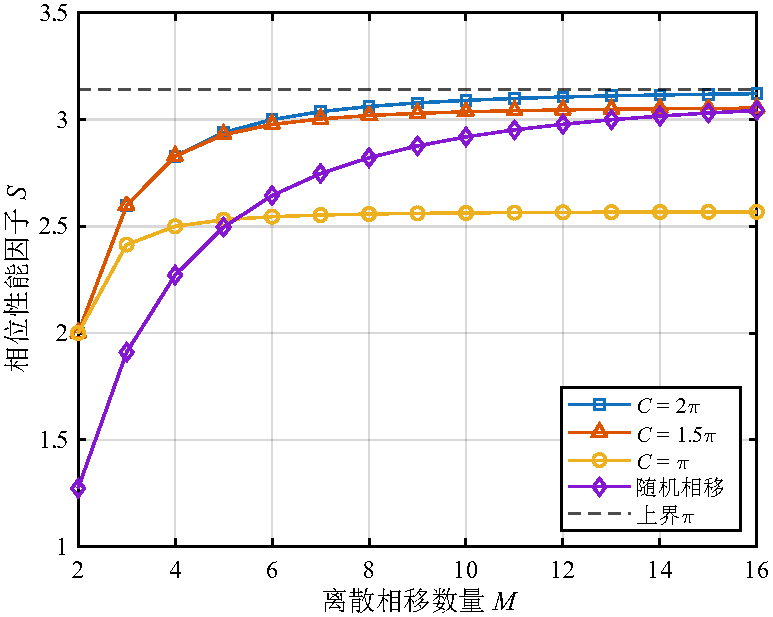
\includegraphics[width=0.6\linewidth]{ddma/ddma_figSvsM.pdf}
	\caption{相位性能因子$\mathcal{S}$随离散相移数量$M$的变化趋势}
	\label{fig:ddma_figSvsM}
\end{figure}

为了直观展示离散相位分布对系统性能的影响，根据定理~\ref{the:ddma_opt_phase}的结论以及随机相位分布的推导结果，图~\ref{fig:ddma_figSvsM}展示了在不同移相能力$C$的约束下，相位性能因子 $\mathcal{S}$ 随离散相位状态数 $M$ 的变化趋势，并与随机相位分布进行了对比。
从图中可以看出，在相同的量化精度下，均匀量化所获得的性能因子 $\mathcal{S}$ 优于随机相移，特别是当 $M$ 较小时，性能差异更加显著，这说明在低分辨率量化场景下有必要对相位分布进行设计。
然而，不同移相能力$C$下的增长速率和性能上界存在明显差异。
当移相能力充足时，$\mathcal{S}$随着$M$的增加逐渐逼近理论上界$\pi$。相反，当移相能力受限时，随着$M$增加，$\mathcal{S}$很快便达到饱和，收敛于一个小于$\pi$的值。
这说明若DMA硬件的调谐范围受限，单纯增加相位控制位数并不能弥补相位覆盖范围不足带来的性能损失。

由于全周期均匀量化是最通用且性能最优的方案，在此场景下，与第\ref{ch:cdma}章类似，将所提CPP算法与直接映射松弛下的量化方法进行对比。结合定理~\ref{the:ddma_gamma_cpp}、定理~\ref{the:ddma_opt_phase}与推论~\ref{cor:cdma_gamma_relax}，得到均匀量化下CPP算法与松弛方法的平均信噪比表达式：
\begin{align}
	\gamma^{\text{CPP}} &= \frac{P_t \rho N_d}{4\sigma^2 N_e} \left( 2a_2 + \frac{\kappa}{\kappa+1} \left[ M\sqrt{\frac{a_2 a_1^2}{\pi}} \sin \frac{\pi}{M} + \frac{M^2(a_1^2-a_2)}{\pi^2} \sin^2 \frac{\pi}{M} \right] \right), \label{eq:ddma_gamma_cpp_uni}\\
	\gamma^{\text{RLX}} &= \frac{P_t \rho N_d}{4\sigma^2 N_e} \left( 2a_2 + \frac{\kappa}{\kappa+1} \left[ \frac{M^2(a_1^2-a_2)}{\pi^2} \sin^2 \frac{\pi}{M} \right] \right). \label{eq:ddma_gamma_rlx_uni}
\end{align}
对比式~\eqref{eq:ddma_gamma_cpp_uni}和式~\eqref{eq:ddma_gamma_rlx_uni}可见，CPP算法相比松弛算法多出了含 $M \sin(\pi/M)$ 的一阶项，这反映了CPP算法在处理离散约束时能够更有效地保留信号的相干叠加增益。
尽管CPP算法展现出了优于传统松弛方法的性能，但其获得的解 $\bm Q^{\text{CPP}}$ 毕竟是基于连续解的直接投影，并非离散约束下的全局最优解。
下述命题给出了在均匀量化的条件下，CPP算法的性能边界。

\begin{proposition}\label{pro:ddma_cpp_bound}
	令 $\bm Q^{\natural}$ 表示在均匀量化约束下优化问题~\eqref{eq:ddma_pQ}的全局最优解。CPP算法获得的解 $\bm Q^{\text{CPP}}$ 与全局最优解的性能比值满足如下界限：
	\begin{equation}
		\cos^2 \left(\frac{\pi}{M}\right) \le \frac{p(\bm Q^{\text{CPP}})}{p(\bm Q^{\natural})} \le 1.
	\end{equation}
\end{proposition}

\begin{proof}
	根据定义，$\bm Q^{\natural}$ 是离散约束下的最优解，而 $\bm Q^\star$ 是无约束连续最优解，显然成立 $p(\bm Q^{\text{CPP}}) \leq p(\bm Q^{\natural}) \leq p(\bm Q^\star)$。因此，只需找到 $p(\bm Q^{\text{CPP}})$ 与 $p(\bm Q^\star)$ 之间的比例关系即可确定下界。
	
	首先，回顾连续最优解对应的目标函数值形式。令 $\Lambda_i = j \sum_{l=1}^{N_{e}} g_{i,l} h_{i,l}$，将定理~\ref{the:cdma_Qstar}中的连续最优相位 $\phi_{i,l}^\star$ 代入目标函数，可得：
	\begin{equation}\label{eq:ddma_p_Qstar}
		p(\bm Q^\star) = \frac{1}{4}\sum_{i=1}^{N_{d}} \left( |\Lambda_i| + \sum_{l=1}^{N_{e}} |g_{i,l} h_{i, l}| \right)^{2}.
	\end{equation}
	接下来计算CPP算法的目标函数值 $p(\bm Q^{\text{CPP}})$：
	\begin{subequations}
		\begin{align}
			p(\bm Q^{\text{CPP}})
			&= \frac{1}{4}\sum_{i=1}^{N_{d}}\left| \Lambda_i +\sum_{l=1}^{N_{e}} g_{i,l} h_{i, l} e^{j \phi_{i,l}^{\text{CPP}}} \right|^{2} \\
			&= \frac{1}{4}\sum_{i=1}^{N_{d}} \left| |\Lambda_i| + \sum_{l=1}^{N_{e}} |g_{i,l} h_{i, l}| e^{j( \phi_{i,l}^{\text{CPP}} - \phi_{i,l}^\star)} \right|^{2} \\
			&\overset{\text{(a)}}{\geq} \frac{1}{4}\sum_{i=1}^{N_{d}} \left( |\Lambda_i| + \sum_{l=1}^{N_{e}} |g_{i,l} h_{i, l}| \cos( \phi_{i,l}^{\text{CPP}} - \phi_{i,l}^\star) \right)^{2} \\
			&\overset{\text{(b)}}{\geq} \frac{1}{4}\sum_{i=1}^{N_{d}} \left( |\Lambda_i| + \sum_{l=1}^{N_{e}} |g_{i,l} h_{i, l}| \cos \left(\frac{\pi}{M}\right) \right)^{2} \\
			&\geq \cos^2 \left(\frac{\pi}{M}\right) \cdot \frac{1}{4} \sum_{i=1}^{N_{d}} \left( |\Lambda_i| + \sum_{l=1}^{N_{e}} |g_{i,l} h_{i, l}|\right)^{2} \\
			&= \cos^2\left(\frac{\pi}{M}\right) p(\bm Q^\star) \geq \cos^2\left(\frac{\pi}{M}\right) p(\bm Q^\natural),
		\end{align}
	\end{subequations}
	其中，步骤(a)利用了复数模值的性质$|z| \ge \text{Re}\{z\}$；步骤(b)基于CPP算法的最近邻投影原则，在均匀量化条件下，任意单元的相位量化误差满足$|\phi_{i,l}^{\text{CPP}} - \phi_{i,l}^\star| \le \frac{\pi}{M}$，结合余弦函数的单调递减性质，有 $\cos( \phi_{i,l}^{\text{CPP}} - \phi_{i,l}^\star) \ge \cos(\frac{\pi}{M})$。证毕。
\end{proof}

命题~\ref{pro:ddma_cpp_bound}确立了CPP算法的性能下界，揭示了其适用范围与局限性。在低分辨率量化场景下，CPP算法的性能保证急剧下降，特别是在1比特量化时，理论下界为 $\cos^2(\pi/2)=0$。这说明在最坏的情况下，算法可能完全失效。
为了在低分辨率量化场景下仍然能获得可观的波束赋形增益，需要探索一种直接针对离散约束进行优化的算法。
下一节将就此展开研究，提出一种基于辅助变量内积最大化的全局最优离散相位优化方案。


\section{角域排序分划搜索算法}\label{sec:ddma_adsps}

本节提出一种角域排序分划搜索算法以解决前述低分辨率量化条件下的性能限制问题。首先引入辅助变量，研究目标函数的几何特性，将离散组合优化问题转化为角域上的单变量优化问题；随后，针对求解过程中计算开销最大的临界角排序环节，利用相位叠加组合的秩-1结构特性，提出了一种基于多路归并的快速排序策略，实现了在多项式时间内的精确求解；进而，针对均匀量化场景，进一步压缩了有效搜索区间。
该算法不仅保证了离散约束下解的最优性，同时将计算复杂度从穷举法的指数级别降低至多项式时间级别。


\subsection{角域问题转化与几何特性}

由于目标函数~\eqref{eq:ddma_pQ}关于不同波导具有可分离性，原问题可分解为 $N_d$ 个独立的子问题。仍然考虑第 $i$ 条波导（$i \in \{1, \dots, N_d\}$）的优化问题，通过提取洛伦兹约束中的常数项并忽略比例因子 $1/4$，该子问题可重写为：
\begin{align}\label{eq:ddma_adsps_P}
	\max_{\{\phi_{i,l}\}} \quad &\left|j \sum_{l=1}^{N_{e}} g_{i,l} h_{i,l} + \sum_{l=1}^{N_{e}} g_{i, l} h_{i, l} e^{j \phi_{i,l}} \right|^{2}, \\
	\text{s.t.} \quad &\phi_{i,l} \in \bm \Phi_M,\; \forall l.
\end{align}
基于式~\eqref{eq:ddma_adsps_P}构建更易于几何分析的实数域形式，定义二维实向量 $\bm c_{i,l} \in \mathbb R^{2 \times 1}$：
\begin{equation}\label{eq:ddma_adsps_c}
	\bm c_{i,l} =
	\begin{cases}
		[\Re\{\Lambda_i\},\Im\{\Lambda_i\}]^\mathrm T,&\text{若}\; l=0, \\
		[\Re\{g_{i,l} h_{i,l}\},\Im\{g_{i,l} h_{i,l}\}]^\mathrm T,&  \text{若}\; 1\le l \le N_e,
	\end{cases}
\end{equation}
其中 $\Lambda_i = j \sum_{l=1}^{N_{e}} g_{i,l} h_{i,l}$ 为第 $i$ 条波导的固有信道项。
进一步地，引入如下的旋转矩阵 $\bm{U}(\phi) \in \mathbb{R}^{2 \times 2}$：
\begin{equation}\label{eq:ddma_adsps_U}
	\bm{U}(\phi_{i,l}) = \begin{bmatrix} \cos\phi_{i,l} & \sin\phi_{i,l} \\ -\sin\phi_{i,l} & \cos\phi_{i,l} \end{bmatrix},
\end{equation}
则第 $i$ 个子问题等价转化为如下的范数最大化形式：
\begin{equation}\label{eq:ddma_adsps_PU}
	\max_{\{\phi_{i,l}\}} \; \left\|\bm{c}_{i,0} + \sum_{l=1}^{N_e} \bm{U}(\phi_{i,l}) \bm{c}_{i,l}\right\|^2,
	\quad \text{s.t.} \; \phi_{i,l} \in \bm \Phi_M,\; \forall l.
\end{equation}

通过引入单位模长的辅助向量 $\bm{t} = [\cos\theta, \sin\theta]^\mathrm{T},\theta \in [0, 2\pi)$，利用柯西-施瓦茨不等式得到范数的变分形式 $\|\bm v\| = \max_{\|\bm t\|=1} \langle \bm v, \bm t \rangle$，目标函数可以等价转化为：
\begin{align}
	\left\|\bm{c}_{i,0} + \sum_{l=1}^{N_e} \bm{U}(\phi_{i,l}) \bm{c}_{i,l}\right\|^2
	&= \left\|\bm{c}_{i,0} + \sum_{l=1}^{N_e} \bm{U}(\phi_{i,l}) \bm{c}_{i,l}\right\|^2 \|\bm{t}\|^2 \\
	&= \max_{\|\bm{t}\| = 1} \left\langle \bm{c}_{i,0} + \sum_{l=1}^{N_e} \bm{U}(\phi_{i,l}) \bm{c}_{i,l}, \bm{t} \right\rangle^2. \label{eq:ddma_adsps_Cauchy}
\end{align}
对于给定的 $\theta$，式~\eqref{eq:ddma_adsps_Cauchy}中的内积项取决于 $\{\phi_{i,l}\}$，定义该内积关于$\theta$的最大值为：
\begin{equation}\label{eq:ddma_adsps_F}
	\mathcal F_i (\theta) \triangleq \max_{\{\phi_{i,l}\}} \left\langle \bm{c}_{i,0} + \sum_{l=1}^{N_e} \bm{U}(\phi_{i,l}) \bm{c}_{i,l}, \bm{t} \right\rangle.
\end{equation}
将向量$\bm{c}_{i,l}$参数化为极坐标的形式 $\bm{c}_{i,l} = \|\bm{c}_{i,l}\| [\cos\vartheta_{i,l},\sin\vartheta_{i,l}]^\mathrm{T}$，根据内积的几何定义，问题~\eqref{eq:ddma_adsps_PU}转化为关于辅助角 $\theta$ 的单变量优化问题：
\begin{equation}\label{eq:ddma_adsps_Ftheta}
	\max_{\theta \in [0, 2\pi)} \mathcal{F}_i(\theta) \triangleq \|\bm{c}_{i,0}\|\cos(\theta - \vartheta_{i,0}) + \sum_{l=1}^{N_e} \|\bm{c}_{i,l}\| \cos(\theta - \vartheta_{i,l} - \check{\phi}_{i,l}),
\end{equation}
其中 $\check{\phi}_{i,l}$ 为给定 $\theta$ 下第 $i$ 条波导上第 $l$ 个单元的最优相位选择：
\begin{equation}\label{eq:ddma_adsps_checkphi}
	\check{\phi}_{i,l} = \mathop{\arg\max}_{\phi_{i,l} \in \bm \Phi_M} \cos(\theta - \vartheta_{i,l} - \phi_{i,l}).
\end{equation}

由式~\eqref{eq:ddma_adsps_checkphi}可知，对于给定的 $\theta$，考虑到相位的离散特性，$\check{\phi}_{i,l}$ 应当使 $\theta$ 与 $\vartheta_{i,l} + \phi_{i,l}$ 之间的角度差最小。
所以当 $\theta$ 连续变化时，仅当其穿过两个相邻离散相位的角平分线时，$\check{\phi}_{i,l}$才会发生跳变，则对于第$i$条波导，所有导致决策跳变的临界角集合$\bm \Theta_i$可表示为：
\begin{equation}\label{eq:ddma_adsps_Theta_i}
	\bm \Theta_i = \left\{ (\vartheta_{i,l} + \frac{\Phi_m + \Phi_{m+1}}{2}) \bmod 2\pi \mid l=1,\dots,N_e, \; m=1,\dots,M \right\}.
\end{equation}
这些临界角将周期 $[0, 2\pi)$分划为最多$MN_e+1$个互不重叠的区间。

为了找到最优的相位配置，需要在整个角域 $\theta \in [0, 2\pi)$ 上进行全面搜索。通过去除重复角度并按升序排列临界角集合 $\bm \Theta_i$，可以构建一系列连续区间：
\begin{equation}\label{eq:ddma_adsps_theta_intervals}
	[\Theta_0, \Theta_1), \cdots, [\Theta_z, \Theta_{z+1}), \cdots, [\Theta_Z, \Theta_{Z+1}),
\end{equation}
其中 $\Theta_0 = 0$，$\Theta_{Z+1} = 2\pi$，且 $Z \le MN_e$。值得注意的是，由于角度的周期性，首区间 $[\Theta_0, \Theta_1)$ 与末区间 $[\Theta_Z, \Theta_{Z+1})$ 在逻辑上是连通的。
在任意一个区间$[\Theta_z, \Theta_{z+1})$内，所有单元的离散相位$\check{\phi}_{i,l}$均保持恒定，从而$\mathcal{F}_i(\theta)$处处可微。对其求导可得：
\begin{equation}\label{eq:ddma_adsps_dF}
	\mathcal{F}_i'(\theta) = -\|\bm{c}_{i,0}\|\sin(\theta - \vartheta_{i,0}) - \sum_{l=1}^{N_e}\|\bm c_{i,l}\|\sin(\theta - \vartheta_{i,l} - \check{\phi}_{i,l}).
\end{equation}
令导数为零，可求得该区间内的唯一驻点$\theta_z^c$：
\begin{equation}\label{eq:ddma_adsps_thetazc}
	\theta_z^c = \arctan\left( \frac{\|\bm c_{i,0}\|\sin\vartheta_{i,0}+\sum_{l=1}^{N_e} \|\bm c_{i,l}\| \sin(\vartheta_{i,l}+\check{\phi}_{i,l})}
	{\|\bm c_{i,0}\|\cos\vartheta_{i,0}+\sum_{l=1}^{N_e} \|\bm c_{i,l}\| \cos(\vartheta_{i,l}+\check{\phi}_{i,l})} \right).
\end{equation}
通过遍历所有临界角以及各区间内部的驻点，必然能在多项式时间内找到 $\mathcal{F}_i(\theta)$ 的全局最大值。

这一策略的实施依赖于对临界角集合$\bm \Theta_i$的有序排列，若直接对 $\bm \Theta_i$ 中 $MN_e$ 个元素进行全排序，其计算复杂度将达到 $\mathcal{O}(MN_e \log(MN_e))$。
为了进一步降低算法开销，下一小节将利用 $\bm \Theta_i$ 的生成结构特性，提出一种高效的快速排序与分划策略。

\subsection{基于外和结构的快速排序与分划}

ADSPS算法的核心挑战在于对每条波导的临界角集合 $\bm \Theta_i$ 进行高效排序，以构建连续的搜索区间。
回顾式~\eqref{eq:ddma_adsps_Theta_i}，临界角集合 $\bm \Theta_i$ 由 $M$ 个离散相位决策边界 $\tau_m=(\Phi_m + \Phi_{m+1})/2$ 与 $N_e$ 个信道相位 $\vartheta_{i,l}$ 两两求和生成。
若将 $\bm \Theta_i$ 视为一个 $N_e \times M$ 的矩阵，其元素$[\bm \Theta_i]_{l,m}$由列向量 $\bm \vartheta_i = [\vartheta_{i,1}, \cdots, \vartheta_{i,N_e}]^\mathrm{T}$ 和行向量 $\bm \tau = [\tau_1, \cdots, \tau_M]$ 的和构成，可表示为：
\begin{equation}
	[\bm \Theta_i]_{l,m} = (\vartheta_{i,l} + \tau_m) \bmod 2\pi.
\end{equation}
从代数结构上看，矩阵 $\bm \Theta_i$ 对应于两个单位模长复向量外积的主辐角，在相位域中，这种特殊的加法结构使得当生成向量有序时，矩阵 $\bm \Theta_i$ 的行或列也呈现出特定的单调性。
利用这一性质，可以避免对所有 $MN_e$ 个元素进行全排序。
鉴于实际应用中通常满足 $N_e \gg M$，本节利用该集合的单调结构特性，提出一种基于多路归并的高效排序策略。

首先，对信道相位向量 $\bm \vartheta_i$ 进行升序排列，得到有序序列 $\tilde{\bm \vartheta}_i$，满足 $0 \le \tilde\vartheta_{i,1} \le \tilde\vartheta_{i,2} \le \cdots \le \tilde\vartheta_{i,N_e} < 2\pi$。对于固定的决策边界索引 $m$，考察生成的子序列 $[\bm \Theta_i]_{l,m} = (\tilde\vartheta_{i,l} + \tau_m) \bmod 2\pi$。由于 $\tilde\vartheta_{i,l} + \tau_m$ 关于 $l$ 单调递增，且 $\tilde\vartheta_{i,l}, \tau_m \in [0, 2\pi)$，其和 $\tilde\vartheta_{i,l} + \tau_m \in [0, 4\pi)$。因此，模 $2\pi$ 运算至多导致一次数值跳变：
\begin{equation}
	[\bm \Theta_i]_{l,m} = 
	\begin{cases} 
		\tilde\vartheta_{i,l} + \tau_m, & \text{若 } \tilde\vartheta_{i,l} + \tau_m < 2\pi, \\ 
		\tilde\vartheta_{i,l} + \tau_m - 2\pi, & \text{若 } \tilde\vartheta_{i,l} + \tau_m \ge 2\pi. 
	\end{cases}
\end{equation}
这说明，虽然子序列 $[\bm \Theta_i]_{l,m}$ 整体上并非单调，但它必定由两个严格单调递增的子段拼接而成：
\begin{align}
	\mathcal{X}_{m,1} &= \{ \tilde\vartheta_{i,1}+\tau_m, \cdots, \tilde\vartheta_{i,l_m}+\tau_m \}, \\
	\mathcal{X}_{m,2} &= \{ \tilde\vartheta_{i,l_m+1}+\tau_m-2\pi, \cdots, \tilde\vartheta_{i,N_e}+\tau_m-2\pi \},
\end{align}
其中，分割点 $l_m$ 是满足 $\tilde\vartheta_{i,l_m} < 2\pi - \tau_m \le \tilde\vartheta_{i,l_m+1}$ 的索引，可通过二分查找确定。
通过上述分析，整个临界角集合 $\bm \Theta_i$ 实际上是由 $2M$ 个有序子序列 $\{\mathcal{X}_{1,1}, \mathcal{X}_{1,2}, \cdots, \mathcal{X}_{M,1}, \mathcal{X}_{M,2}\}$ 构成的。
这一结构特性可以使用多路归并加速排序：维护一个大小为 $2M$ 的最小堆，用于动态管理当前所有非空子序列的队首元素。首先，将所有 $2M$ 个子序列的首元素及其所属序列号压入堆中。随后，执行 $MN_e$ 次迭代：每次弹出堆顶元素，存入结果数组 $\tilde{\bm \Theta}_{i}$；若该元素所属子序列仍有剩余元素，则读取该序列的下一元素并压入堆中，直到所有子序列均为空，完成最终的排序。


\begin{algorithm}[!t]
	\caption{角域排序分划搜索算法（ADSPS）}
	\label{alg:ddma_adsps}
	\begin{algorithmic}[1]
		\REQUIRE 信道 $\bm g$，传输矩阵 $\bm H$，离散相移$\bm \Phi_M$，离散阶数 $M$，波导数$N_d$，单元数$N_e$。
		\ENSURE 全局最优DMA配置矩阵 $\bm Q^{\natural}$。
		\STATE 初始化 $\bm Q^{\natural} = \bm 0_{N \times N_d}$；
		\FOR {$i = 1, 2, \cdots, N_d$}
		\STATE 根据式~\eqref{eq:ddma_adsps_c}计算 $\bm c_{i,l}$ 及相位 $\vartheta_{i,l}$，计算决策偏移量 $\tau_m$；
		\STATE 对 $\{\vartheta_{i,1}, \dots, \vartheta_{i,N_e}\}$ 进行升序排序得到 $\tilde{\bm \vartheta}_i$；
		\STATE 初始化最小堆 $H = \emptyset$，有序临界角结果数组 $\tilde{\bm \Theta}_{i} = []$；
		\FOR {$m = 1$ to $M$}
		\STATE 在 $\tilde{\bm \vartheta}_i$ 中二分查找分割点 $l_m$，满足 $\tilde\vartheta_{i,l_m} < 2\pi - \tau_m \le \tilde\vartheta_{i,l_m+1}$；
		\STATE 构建子序列 $\mathcal{X}_{m,1}$ 和 $\mathcal{X}_{m,2}$；
		\STATE 若 $\mathcal{X}_{m,1}$ 或 $\mathcal{X}_{m,2}$ 非空，则将其首元素及其所属序列号ID压入堆$H$；
		\ENDFOR
		\WHILE {$H$ 非空}
		\STATE 弹出堆顶元素 $(\theta, \text{ID})$，将 $\theta$ 追加至 $\tilde{\bm \Theta}_{i}$；
		\STATE 若序列 $\text{ID}$ 仍有后继元素，读取下一元素并压入堆 $H$；
		\ENDWHILE
		\STATE 去除有序集合 $\tilde{\bm \Theta}_{i}$中的重复元素，根据式~\eqref{eq:ddma_adsps_theta_intervals}构建区间序列；
		\FOR {每个有效区间$[\Theta_z, \Theta_{z+1})$}
		\STATE 根据式~\eqref{eq:ddma_adsps_checkphi}确定区间内的离散相位配置$\{\check{\phi}_{i,l}\}$；
		\STATE 利用式~\eqref{eq:ddma_adsps_thetazc}计算驻点 $\theta_z^c$；
		\IF {$\theta_z^c \in (\Theta_z, \Theta_{z+1})$}
		\STATE 计算目标函数值$\mathcal{F}_i(\theta_z^c)$；
		\ENDIF
		\STATE 与区间端点的函数值比较，得到区间内的最大值及对应的最优角 $\theta^{\natural}$；
		\ENDFOR
		\STATE 根据全局最大值对应的$\theta^{\natural}$反解最优离散相位$\{{\phi}_{i,l}^{\natural}\}$，更新 $[\bm Q^{\natural}]_{(i-1)N_e+1:iN_e, i}$；
		\ENDFOR
		\RETURN $\bm Q^{\natural}$。
	\end{algorithmic}
\end{algorithm}

综合上述分析，对每个波导进行分化搜索，可得到问题~\eqref{eq:ddma_pQ}的全局最优解$\bm Q^{\natural}$。
ADSPS算法的完整流程如算法~\ref{alg:ddma_adsps}所示。
下面对该算法的计算复杂度进行详细分析。
ADSPS算法的计算开销由临界角排序与区间搜索两个阶段共同决定。
对于单个波导子问题，在排序阶段主要有预排序、虚拟分割和多路归并这三个步骤：对长度为 $N_e$ 的信道相位向量进行预排序，复杂度为 $\mathcal{O}(N_e \log N_e)$；
在查找定位分割点 $l_m$中，需要执行 $M$ 次二分查找，每次查找长度为 $N_e$，复杂度为 $\mathcal{O}(M \log N_e)$；在归并排序中，共进行了$MN_e$次堆的插入与删除操作，堆的大小维持在 $2M$，单次操作复杂度为 $\mathcal{O}(\log M)$，总归并复杂度为 $\mathcal{O}(MN_e \log M)$。
相较于对所有元素进行全排序，该策略实现了显著的复杂度下降。
随后进入区间搜索，算法在生成的至多 $MN_e+1$ 个连续区间 $[\Theta_z, \Theta_{z+1})$ 内进行搜索，在每个有效区间内，需要依据式~\eqref{eq:ddma_adsps_thetazc}计算驻点 $\theta_z^c$ 并评估目标函数值。
当辅助角 $\theta$ 跨越任意临界角进入相邻区间时，仅有一个特定天线单元的离散最优相位 $\check{\phi}_{i,l}$ 会发生跳变，因此，可以采用增量更新机制来计算式~\eqref{eq:ddma_adsps_thetazc}中的三角函数求和项，使得单次区间切换和驻点计算的复杂度仅为$\mathcal{O}(1)$。基于此滑动窗口式的计算策略，整个区间搜索阶段的计算复杂度为 $\mathcal{O}(MN_e)$。
考虑到原问题由 $N_d$ 条相互独立的波导构成，所提ADSPS算法的整体计算复杂度最终可表示为：
\begin{equation}\label{eq:ddma_adsps_complexity}
	\mathcal{O}\left( N_d (N_e \log N_e + M \log N_e + MN_e \log M + MN_e) \right).
\end{equation}
相比之下，若采用传统的穷举搜索法直接在离散相位集合 $\bm \Phi_M$ 中寻找每条波导的最优配置，其计算复杂度为 $\mathcal{O}(N_d M^{N_e})$。
ADSPS算法不仅在理论上严格保证了离散量化约束下波束赋形解的全局最优性，更将问题的计算开销从穷举法的指数级别降低至多项式级别。

\subsection{均匀量化下的搜索空间分析}

尽管ADSPS算法在一般任意离散相移场景下已经具备了多项式级别的计算复杂度，但对于实际中应用最广泛的均匀量化情形，最优解的搜索空间可以进一步压缩。下述命题给出了精简后的有效搜索空间。

\begin{proposition}\label{pro:ddma_thetaFlat}
	若离散相位集合 $\bm \Phi_M$ 为均匀分布，令 $\theta_i^{\natural} = \mathop{\arg\max}_{\theta \in [0,2\pi)} \mathcal{F}_i(\theta)$ 为第 $i$ 条波导对应的最优辅助角。
	则$\theta_i^\natural$必然位于以下区间内：
	\begin{equation}\label{eq:ddma_thetaFlatin}
		\theta_i^{\natural} \in
		\begin{cases}
			[0,\vartheta_{i,0}+\frac{\pi}{M})\cup(\vartheta_{i,0}-\frac{\pi}{M}+2\pi,2\pi), & \text{若}\; \vartheta_{i,0} < \frac{\pi}{M}, \\
			[0,\vartheta_{i,0}+\frac{\pi}{M}-2\pi)\cup(\vartheta_{i,0}-\frac{\pi}{M},2\pi), & \text{若}\; \vartheta_{i,0} > 2\pi- \frac{\pi}{M}, \\
			(\vartheta_{i,0}-\frac{\pi}{M}, \vartheta_{i,0}+\frac{\pi}{M}), & \text{其他情况}.
		\end{cases}
	\end{equation}
	更进一步地，假设 $\mathcal{F}_i(\theta)$ 在区间 $[\Theta_z, \Theta_{z+1})$ 内取得全局最大值，则必有：
	\begin{equation}\label{eq:ddma_thetaFlatzc}
		\theta_i^{\natural} = \theta_z^c \in (\Theta_z, \Theta_{z+1}),
	\end{equation}
	即最优解总是位于某个区间的内部，而不会落在任意区间的边界端点上。
\end{proposition}

\begin{proof}
	首先证明式~\eqref{eq:ddma_thetaFlatin}的邻域约束。由反证法，根据式~\eqref{eq:ddma_adsps_Ftheta}，将目标函数分解为常数信道项与可调相位项之和，定义辅助函数：
	\begin{equation}\label{eq:ddma_F0}
		\mathcal F_{i,0}(\theta) = \sum_{l=1}^{N_e} \|\bm{c}_{i,l}\| \cos(\theta - \vartheta_{i,l} - \check{\phi}_{i,l}),
	\end{equation}
	则原目标函数可表示为 $\mathcal F_i(\theta) = \|\bm{c}_{i,0}\| \cos(\theta - \vartheta_{i,0}) + \mathcal F_{i,0}(\theta)$。
	由于均匀量化集合中相位的等间隔特性，对于任意给定的 $\theta$，将其平移 $2\pi/M$ 的整数倍后，所有单元的量化决策 $\check{\phi}_{i,l}$ 也会随之同步发生 $2\pi/M$ 的循环移位，因此，辅助函数 $\mathcal F_{i,0}(\theta)$ 是一个周期为 $2\pi/M$ 的周期函数。
	假设$\theta_i^{\natural} = \mathop{\arg\max}_{\theta \in [0,2\pi)} \mathcal{F}_i(\theta)$，有：
	\begin{equation}\label{eq:ddma_F0flat}
		\mathcal F_{i,0}(\theta_i^{\natural}) = \mathcal F_{i,0}\left(\theta_i^{\natural} + \frac{2\pi}{M}\right) = \cdots = \mathcal F_{i,0}\left(\theta_i^{\natural} + \frac{2(M-1)\pi}{M}\right).
	\end{equation}
	
	假设$\theta_i^{\natural}$ 落在了式~\eqref{eq:ddma_thetaFlatin}所定义的区间之外，则必然存在一个整数$m$，使得平移后的角度 $\theta_i^{\natural} + \frac{2m\pi}{M}$ 恰好落入式~\eqref{eq:ddma_thetaFlatin}所定义的区间内。
	此时，由于平移后的角度更接近 $\vartheta_{i,0}$，余弦函数的单调性决定了 $\cos(\theta_i^{\natural} + \frac{2m\pi}{M} - \vartheta_{i,0}) > \cos(\theta_i^{\natural} - \vartheta_{i,0})$。
	结合式~\eqref{eq:ddma_F0flat}，可推得 $\mathcal{F}_i(\theta_i^{\natural} + \frac{2m\pi}{M}) > \mathcal{F}_i(\theta_i^{\natural})$。
	这与 $\theta_i^{\natural}$ 是 $\mathcal{F}_i(\theta)$ 全局最大值点的假设相矛盾。因此，式~\eqref{eq:ddma_thetaFlatin}得证。
	
	接下来证明式~\eqref{eq:ddma_thetaFlatzc}，回顾式~\eqref{eq:ddma_adsps_Cauchy}的推导，$\mathcal{F}_i(\theta)$取得最大值等价于柯西-施瓦茨不等式取等号。
	这意味着合成向量 $\bm{c}_{i,0} + \sum_{l=1}^{N_e} \bm{U}(\phi_{i,l}) \bm{c}_{i,l}$ 与辅助向量 $\bm{t}$ 平行，从而最大值只能在内部驻点 $\theta_z^c$ 处取得。
	现在进一步排除驻点$\theta_z^c$恰好落在区间端点$\Theta_z$的可能性。
	再次采用反证法，假设 $\theta_i^{\natural} = \Theta_z = \vartheta_{i,l} + \frac{(2m-1)\pi}{M}$，即最大值在第 $l$ 个单元的第 $m$ 个决策边界处取得。
	在此假设下，$\check{\phi}_{i,l}$ 的取值为 $\frac{2(m-1)\pi}{M}$ 或 $\frac{2m\pi}{M}$。
	构造剔除第 $l$ 个单元影响的剩余函数：
	\begin{equation}\label{eq:ddma_Fil}
		\mathcal F_{i,l}(\theta) = \mathcal F_i(\theta) - \|\bm{c}_{i,l}\| \cos(\theta - \vartheta_{i,l} - \check{\phi}_{i,l}).
	\end{equation}
	
	易知 $\mathcal{F}_{i,l}(\theta)$ 在 $\theta = \Theta_z$ 处是连续且可导的。
	当从左侧逼近边界时，$\check{\phi}_{i,l} = \frac{2(m-1)\pi}{M}$，此时原函数$\mathcal{F}_i(\theta)$在 $\Theta_z$ 处的左导数为：
	\begin{equation}
		\mathcal{F}_{i-}'(\Theta_z) = \mathcal{F}_{i,l}'(\Theta_z) - \|\bm{c}_{i,l}\| \sin\left(\frac{\pi}{M}\right) = 0.
	\end{equation}
	而当从右侧逼近边界时，$\check{\phi}_{i,l} = \frac{2m\pi}{M}$，对应的右导数为：
	\begin{equation}
		\mathcal{F}_{i+}'(\Theta_z) = \mathcal{F}_{i,l}'(\Theta_z) + \|\bm{c}_{i,l}\| \sin\left(\frac{\pi}{M}\right) > 0.
	\end{equation}
	右导数大于零表明函数$\mathcal{F}_i(\theta)$在穿过 $\Theta_z$ 后将继续增加，这与 $\Theta_z$ 为局部最大值点的假设矛盾。同理，若设定右导数为零，则推得左导数小于零，同样导致矛盾。因此，最优角 $\theta_i^{\natural}$ 必然严格位于某开区间 $(\Theta_z, \Theta_{z+1})$ 的内部。
\end{proof}

命题~\ref{pro:ddma_thetaFlat}表明，在均匀量化下，有效搜索区域的角域宽度被限制为 $2\pi/M$，每个天线单元有且仅有一个临界角会落入该有效邻域内。相较于原始至多$MN_e$个分划区间，落入该有效邻域内的区间数量大幅下降至仅约$N_e+1$个。对这些筛选出的有效临界角进行局部排序的复杂度为$\mathcal{O}(N_e \log N_e)$。
其次，式~\eqref{eq:ddma_thetaFlatzc}明确了极值点不会出现在边界上。因此，在遍历有效区域内的区间 $[\Theta_z, \Theta_{z+1})$ 时，只需简单检验计算得到的驻点 $\theta_z^c$ 是否满足 $\theta_z^c \in (\Theta_z, \Theta_{z+1})$ 即可。若不满足，则直接舍弃该候选点；若满足，则保留并计算对应的函数值 $\mathcal{F}_i(\theta_z^c)$。
整个搜索阶段的复杂度也相应降低至$\mathcal{O}(N_e)$。
因此，考虑$N_d$条波导，针对均匀量化条件精简后的ADSPS算法的整体计算复杂度可表示为$\mathcal{O}\left( N_d (N_e \log N_e + N_e) \right)$。

\subsection{算法性能下界分析}

前述小节从理论上证明了ADSPS算法能在多项式时间内寻找到离散量化约束下的全局最优解，并大幅降低了计算复杂度。
为了进一步从理论层面揭示该算法相比最近点投影算法在低分辨率量化条件下的鲁棒性与性能优势，本小节将对其波束赋形增益的性能下界展开推导与分析。

首先考虑1-bit均匀量化情况，离散相位集合$\bm \Phi_2 = \{0, \pi\}$是目前应用最广泛的低分辨率配置。
此时，目标函数$\mathcal F_{i}(\theta)$退化为：
\begin{equation}\label{eq:ddma_Fi_theta_1bit}
	\mathcal F_{i}(\theta) = \sum_{l=0}^{N_e} \|\bm{c}_{i,l}\| |\cos(\theta - \vartheta_{i,l})|.
\end{equation}
该函数可视为在辅助角 $\theta$上各天线单元信道向量投影绝对值之和。通过相似的一维连续搜索，ADSPS算法能够协调所有天线单元的符号选择。下面通过命题的形式给出其在1比特情形的性能下界。

\begin{proposition}\label{pro:ddma_adsps_1bit_bound}
	对于1比特均匀量化情形，设 $\bm Q^{\natural}$ 为采用ADSPS算法获得的离散全局最优配置矩阵，$\bm Q^{\star}$ 为无约束连续最优配置矩阵。则ADSPS算法的目标性能满足以下界限：
	\begin{equation}
		p(\bm Q^{\natural}) \ge \frac{1}{4} p(\bm Q^{\star}).
	\end{equation}
\end{proposition}

\begin{proof}
	两相位均匀量化下第 $i$ 条波导的最大化子问题等价于求 $\max_{\theta \in [0, 2\pi)} |\mathcal F_i(\theta)|^2$。
	由于对于任意实数 $x \in [-1, 1]$ 均有 $|x| \ge x^2$ 成立，根据式~\eqref{eq:ddma_Fi_theta_1bit}，利用该不等式放缩 $|\cos(\theta - \vartheta_{i,l})|$，目标函数的最大值可建立如下界限：
	\begin{align}
		\max_{\theta \in [0, 2\pi)} \left| \mathcal F_i(\theta) \right|^2 
		&= \max_{\theta \in [0, 2\pi)} \left| \sum_{l=0}^{N_e} \|\bm c_{i,l}\| |\cos(\theta - \vartheta_{i,l})| \right|^2 \nonumber \\
		&\ge \max_{\theta \in [0, 2\pi)} \left| \sum_{l=0}^{N_e} \|\bm c_{i,l}\| \cos^2(\theta - \vartheta_{i,l}) \right|^2 \nonumber \\
		&= \max_{\theta \in [0, 2\pi)} \left| \sum_{l=0}^{N_e} \|\bm c_{i,l}\| \frac{1 + \cos(2(\theta - \vartheta_{i,l}))}{2} \right|^2 \nonumber \\
		&= \medmath{\max_{\theta \in [0, 2\pi)} \left| \sum_{l=0}^{N_e} \frac{\|\bm c_{i,l}\|}{2} + \sum_{l=0}^{N_e} \frac{\|\bm c_{i,l}\|}{2} \cos(2\vartheta_{i,l})\cos(2\theta) + \sum_{l=0}^{N_e} \frac{\|\bm c_{i,l}\|}{2} \sin(2\vartheta_{i,l})\sin(2\theta) \right|^2}. \label{eq:ddma_proof_1bit_expand}
	\end{align}
	对于式~\eqref{eq:ddma_proof_1bit_expand}中的后两项，总可以找到一个特定的辅助角 $\theta \in [0, 2\pi)$，使得 $\cos(2\theta)$ 和 $\sin(2\theta)$ 分别与常数系数 $\sum_{l=0}^{N_e} \frac{\|\bm c_{i,l}\|}{2} \cos(2\vartheta_{i,l})$ 和 $\sum_{l=0}^{N_e} \frac{\|\bm c_{i,l}\|}{2} \sin(2\vartheta_{i,l})$ 具有相同的符号。
	这说明在该特定的 $\theta$ 处，这两项分量之和必定非负。
	因此，该式在整个周期上的最大值必定不小于第一项常数分量：
	\begin{equation}\label{eq:ddma_proof_1bit_final}
		\max_{\theta \in [0, 2\pi)} \left| \mathcal F_i(\theta) \right|^2 \ge \left| \sum_{l=0}^{N_e} \frac{\|\bm c_{i,l}\|}{2} \right|^2 = \frac{1}{4} \left( \sum_{l=0}^{N_e} \|\bm c_{i,l}\| \right)^2.
	\end{equation}
	将式~\eqref{eq:ddma_proof_1bit_final}代入系统整体目标函数 $p(\bm Q^{\natural}) = \frac{1}{4} \sum_{i=1}^{N_d} \max_\theta (\mathcal F_i(\theta))^2$ 中，并对照式~\eqref{eq:ddma_p_Qstar}中无约束连续最优目标函数 $p(\bm Q^{\star})$ 的表达式，直接可得 $p(\bm Q^{\natural}) \ge \frac{1}{4} p(\bm Q^{\star})$。证毕。
\end{proof}

命题~\ref{pro:ddma_adsps_1bit_bound}证实了在1比特量化下，ADSPS算法仍能保证获得理想连续相移情形$25\%$以上的波束赋形增益，而前节CPP算法的理论性能下界为 $\cos^2(\pi/2) = 0$。这是因为CPP算法仅对各单元相位进行孤立的就近量化投影，当信道相位恰好处于量化死区边缘时，容易引起各个单元的相消叠加；而ADSPS算法通过在角域 $[0, 2\pi)$ 上的全局协同搜索，有效避免了这种情况的发生。
在上述代数不等式推导的基础上，进一步放宽对量化阶数的限制，可以推导任意$M$阶均匀量化下ADSPS算法的普遍性能下界。

\begin{proposition}\label{pro:ddma_adsps_Mbit_bound}
	对于任意离散阶数 $M \ge 2$ 的均匀量化情形，ADSPS算法获得的离散最优目标函数值 $p(\bm Q^{\natural})$ 与无约束连续最优值 $p(\bm Q^{\star})$ 满足如下界限：
	\begin{equation}\label{eq:ddma_adsps_Mbit_bound}
		p(\bm Q^{\natural}) \ge \left( \frac{M}{\pi} \sin \frac{\pi}{M} \right)^2 p(\bm Q^{\star}).
	\end{equation}
\end{proposition}

\begin{proof}
	对于任意波导$i$，根据式~\eqref{eq:ddma_adsps_Ftheta}和命题~\ref{pro:ddma_thetaFlat}的结论，在均匀量化条件下，最优辅助角 $\theta_i^{\natural}$ 必定落入以常数信道求和项的相位 $\vartheta_{i,0}$为中心、宽度为$2\pi/M$的有效搜索邻域内。
	不失一般性，可将该连通的有效搜索区间等效记为 $\mathcal{I}_i = [\vartheta_{i,0} - \frac{\pi}{M}, \vartheta_{i,0} + \frac{\pi}{M}]$。
	
	既然全局最大值必定在该区间 $\mathcal{I}_i$ 内取得，那么目标函数的全局最大值自然不小于其在该特定局部区间上的积分平均值，即：
	\begin{equation}
		\max_{\theta \in [0, 2\pi)} \mathcal F_i(\theta) = \max_{\theta \in \mathcal{I}_i} \mathcal F_i(\theta) \ge \frac{M}{2\pi} \int_{\vartheta_{i,0} - \frac{\pi}{M}}^{\vartheta_{i,0} + \frac{\pi}{M}} \mathcal F_i(\theta) \, \mathrm{d}\theta.
	\end{equation}
	分别对常数项和可调相位项进行区间积分计算，对于常数信道求和项，其在区间 $\mathcal{I}_i$ 上的积分为：
	\begin{equation}
		\frac{M}{2\pi} \int_{\vartheta_{i,0} - \frac{\pi}{M}}^{\vartheta_{i,0} + \frac{\pi}{M}} \|\bm c_{i,0}\| \cos(\theta - \vartheta_{i,0}) \, \mathrm{d}\theta  
		= \|\bm c_{i,0}\| \frac{M}{\pi} \sin \frac{\pi}{M}.
	\end{equation}
	对于第 $l$ 个可调相位项，根据式~\eqref{eq:ddma_adsps_checkphi}中离散相位 $\check{\phi}_{i,l}$ 的最优决策准则，在均匀量化条件下，连续相位 $(\theta - \vartheta_{i,l})$ 与其最优离散选择 $\check{\phi}_{i,l}$ 之间的量化误差是一个关于 $\theta$ 的周期函数，其周期恰为 $2\pi/M$。
	由于积分区间 $\mathcal{I}_i$ 的长度正好涵盖一个完整的周期，该项在 $\mathcal{I}_i$ 上的积分不受信道相位偏移的影响，恒等于余弦函数在标准量化误差区间 $[-\frac{\pi}{M}, \frac{\pi}{M}]$ 上的积分：
	\begin{equation}
		\frac{M}{2\pi} \int_{\mathcal{I}_i} \|\bm c_{i,l}\| \cos(\theta - \vartheta_{i,l} - \check{\phi}_{i,l}) \, \mathrm{d}\theta = \|\bm c_{i,l}\| \frac{M}{2\pi} \int_{-\frac{\pi}{M}}^{\frac{\pi}{M}} \cos(x) \, \mathrm{d}x = \|\bm c_{i,l}\| \frac{M}{\pi} \sin \frac{\pi}{M}.
	\end{equation}
	合并以上各项，可得：
	\begin{equation}
		\max_{\theta \in [0, 2\pi)} \mathcal F_i(\theta) \ge \left( \frac{M}{\pi} \sin \frac{\pi}{M} \right) \left( \|\bm c_{i,0}\| + \sum_{l=1}^{N_e} \|\bm c_{i,l}\| \right).
	\end{equation}
	对上式两侧进行平方，并对所有波导 $i=1,\dots,N_d$ 求和。最后，代入系统总目标函数$p(\bm Q)$并对照式~\eqref{eq:ddma_p_Qstar}，即证得式~\eqref{eq:ddma_adsps_Mbit_bound}。
\end{proof}

对比上述两个命题可以发现，基于局部积分均值特性推导的命题~\ref{pro:ddma_adsps_Mbit_bound}提供了一个更为普适且紧致的下界，证明了所提ADSPS算法的性能下限由于启发式的CPP算法。
随着量化阶数 $M$ 的增加，下界因子 $( \frac{M}{\pi} \sin \frac{\pi}{M} )^2$ 将迅速逼近 1，说明ADSPS算法在高分辨率条件下能快速逼近连续最优解。


\noindent\rule{\linewidth}{2pt}





\section{数值仿真分析}

\section{本章小结}

\textcolor{red}{之后再写}




%由于 $a_1, a_2, M$ 均为正数，这从理论上直接证明了在相同的量化条件下，CPP算法能够获得比松弛算法更高的波束赋形增益。为了量化评估相位离散化带来的性能折损，定义连续相移下的理想平均信噪比为 $\gamma^\star \triangleq \lim_{M \to \infty} \gamma^{\text{CPP}}_{\text{uni}}$。利用极限 $\lim_{M \to \infty} M \sin(\frac{\pi}{M}) = \pi$，可得：
%\begin{equation}\gamma^\star = \frac{P_t \rho N_d}{4\sigma^2 N_e}\left(2a_2+\frac{\kappa}{\kappa+1} \left(\sqrt{\pi a_2 a_1^2}+a_1^2-a_2\right)\right).\end{equation}
%进一步定义量化性能损失比 $\varepsilon \triangleq \frac{\gamma}{\gamma^\star}$，其中 $\gamma$ 可取 $\gamma^{\text{CPP}}_{\text{uni}}$ 或 $\gamma^{\text{Rel}}_{\text{uni}}$。图~\ref{fig:performance_loss}展示了在不同单元数 $N_e$ 配置下，CPP算法、松弛算法以及随机相位方法的性能损失 $\varepsilon$ 随量化比特数（即状态数 $M$）的变化趋势。图中随机方法的性能下界由式~\eqref{eq:ddma_ESrandom_closed_floor}计算所得。
%
%\begin{figure}[!htbp]\centering
%	\caption{不同算法的性能损失 $\varepsilon$ 随离散相位状态数 $M$ 的变化对比 ($\kappa=10$, $\alpha = 0.6$ m$^{-1}$, $D = 0.0054$ m)}\label{fig:performance_loss}\end{figure}
%
%从图~\ref{fig:performance_loss}的数值结果可以得出以下分析结论：首先，CPP算法在所有配置下均显著优于松弛算法。尤其是在低量化精度（如 $M$ 较小）和波导单元数 $N_e$ 较少的情况下，CPP算法的优势更为明显。例如，当 $N_e=8$ 且 $M$ 趋于无穷大时，CPP算法相比松弛算法仍保持约 2.1 dB 的性能增益；即使当 $N_e$ 增加至 32 时，该增益仍维持在 1.3 dB 左右。这说明直接针对离散约束进行最近点投影（CPP），相比于先在松弛域求解再量化（Relaxation），能更有效地保留信号的相干叠加增益。其次，量化损失随分辨率提高而快速收敛。对于CPP算法，当 $M=8$（即3比特量化）时，性能损失已趋近于 0 dB，意味着此时系统性能已非常接近连续相移的理想情况。这为实际工程设计提供了重要参考：采用 3 比特或 4 比特的低成本移相器即可满足大部分DMA系统的性能需求。
%最后，单元规模 $N_e$ 对量化敏感度有影响。对比不同 $N_e$ 的曲线可知，随着单条波导上单元数量的增加，系统对相位误差的敏感度降低，量化损失收敛速度加快。然而，对于松弛算法和随机方法，随着 $N_e$ 的增加（即 $N_e \to \infty$），其性能损失反而趋于一个较大的常数（例如随机方法在 $N_e \to \infty$ 时损失高达 24.8 dB），这进一步凸显了在大规模DMA阵列中采用高效波束赋形算法（如CPP）的必要性。
%
%\noindent\rule{\linewidth}{2pt}
%
%为了定量量化效应带来的性能损失，定义连续相移条件下的极限信噪比 $\gamma^\star \triangleq \lim_{M \to \infty} \gamma^{\text{CPP}}$ 作为性能基准：
%\begin{equation}
%	\gamma^\star = \frac{P_t \rho N_d}{4\sigma^2 N_e} \left( 2a_2 + \frac{\kappa}{\kappa+1} \left[ \sqrt{\pi a_2 a_1^2} + a_1^2 - a_2 \right] \right).
%\end{equation}
%相应地，定义量化性能损失因子为 $\varepsilon \triangleq \gamma / \gamma^\star$。
%
%\begin{figure}[!htbp]
%	\centering
%	\caption{不同算法的性能损失 $\varepsilon$ 随离散相移数量 $M$ 和单元数 $N_e$ 的变化关系}
%	\label{fig:ddma_performance_loss}
%\end{figure}
%
%图~\ref{fig:ddma_performance_loss}展示了CPP算法与松弛算法的性能损失 $\varepsilon$ 随离散相移数量 $M$ 及每个波导单元数 $N_e$ 的变化趋势。图中还绘制了随机相位方法的性能作为下界参考。
%从量化精度的角度看，随着 $M$ 的增加，CPP算法的性能损失显著降低，迅速逼近连续相移基准。特别是在 $N_e \to \infty$ 这一“最差”量化场景下（即单元数众多导致累积量化误差影响最大），3位量化（$M=8$）的性能损失仅为 $0.22\text{ dB}$，而2位量化（$M=4$）的损失也仅为 $0.87\text{ dB}$。这表明在实际工程中，采用3位精度的离散DMA即可获得接近理想连续系统的性能，在硬件成本与系统性能之间取得了良好的折中。
%
%从算法对比的角度分析，CPP算法在各种配置下均优于传统的松弛算法。
%对比式~\eqref{eq:ddma_gamma_cpp_uni}与式~\eqref{eq:ddma_gamma_rel_uni}可知，CPP算法的优势主要来源于信噪比表达式中包含的 $M \sin(\pi/M)$ 一次项，该项反映了CPP算法在处理离散约束时能够更有效地保留信号的相干叠加增益。
%如图所示，当 $N_e=8$ 时，CPP算法相比松弛算法有约 $2.1\text{ dB}$ 的性能优势；即使在 $N_e$ 增大至 $32$ 时，优势依然维持在 $1.3\text{ dB}$ 左右。
%这证明了CPP算法虽然计算简单，但在处理非凸的离散相位约束时，能够比直接量化的松弛方法更精准地逼近全局最优解，具有显著的性能优越性。




\chapter{捏合天线波束赋形性能分析与几何辅助定位算法}\label{ch:pass}

\section{引言}

\textcolor{red}{之后再写}

\section{系统模型}

\subsection{系统模型}

本章考虑一个典型的基于捏合天线的上行通信系统。如图~\ref{fig:pass_structure}所示，系统由$M$条介质波导组成，波导均沿$x$轴方向铺设，长度为$L_x$，并在$y$轴方向上均匀分布于区间$[0, L_y]$内，即相邻两条波导之间的间距为$L_y/(M-1)$。所有波导位于高度为$L_z$的水平平面上，每条波导上部署一个可沿波导方向连续滑动的捏合天线。
建立图示的坐标系，第$m$个捏合天线的位置坐标可表示为$\bm{p}_m = [x_m, y_m, z_m]^{\mathrm{T}}$。其中，$x_m \in [0, L_x]$为该天线在波导上可动态调节的滑动位置，$y_m = \frac{L_y(m-1)}{M-1}$为其固定的纵坐标，$z_m = L_z$为波导所在平面的高度。假设单天线用户终端位于地面，其位置坐标表示为$\bm{p}_U = [u, v, 0]^{\mathrm{T}}$，其中$u \in [0, L_x]$，$v \in [0, L_y]$。

\begin{figure}[!htbp]
	\centering
	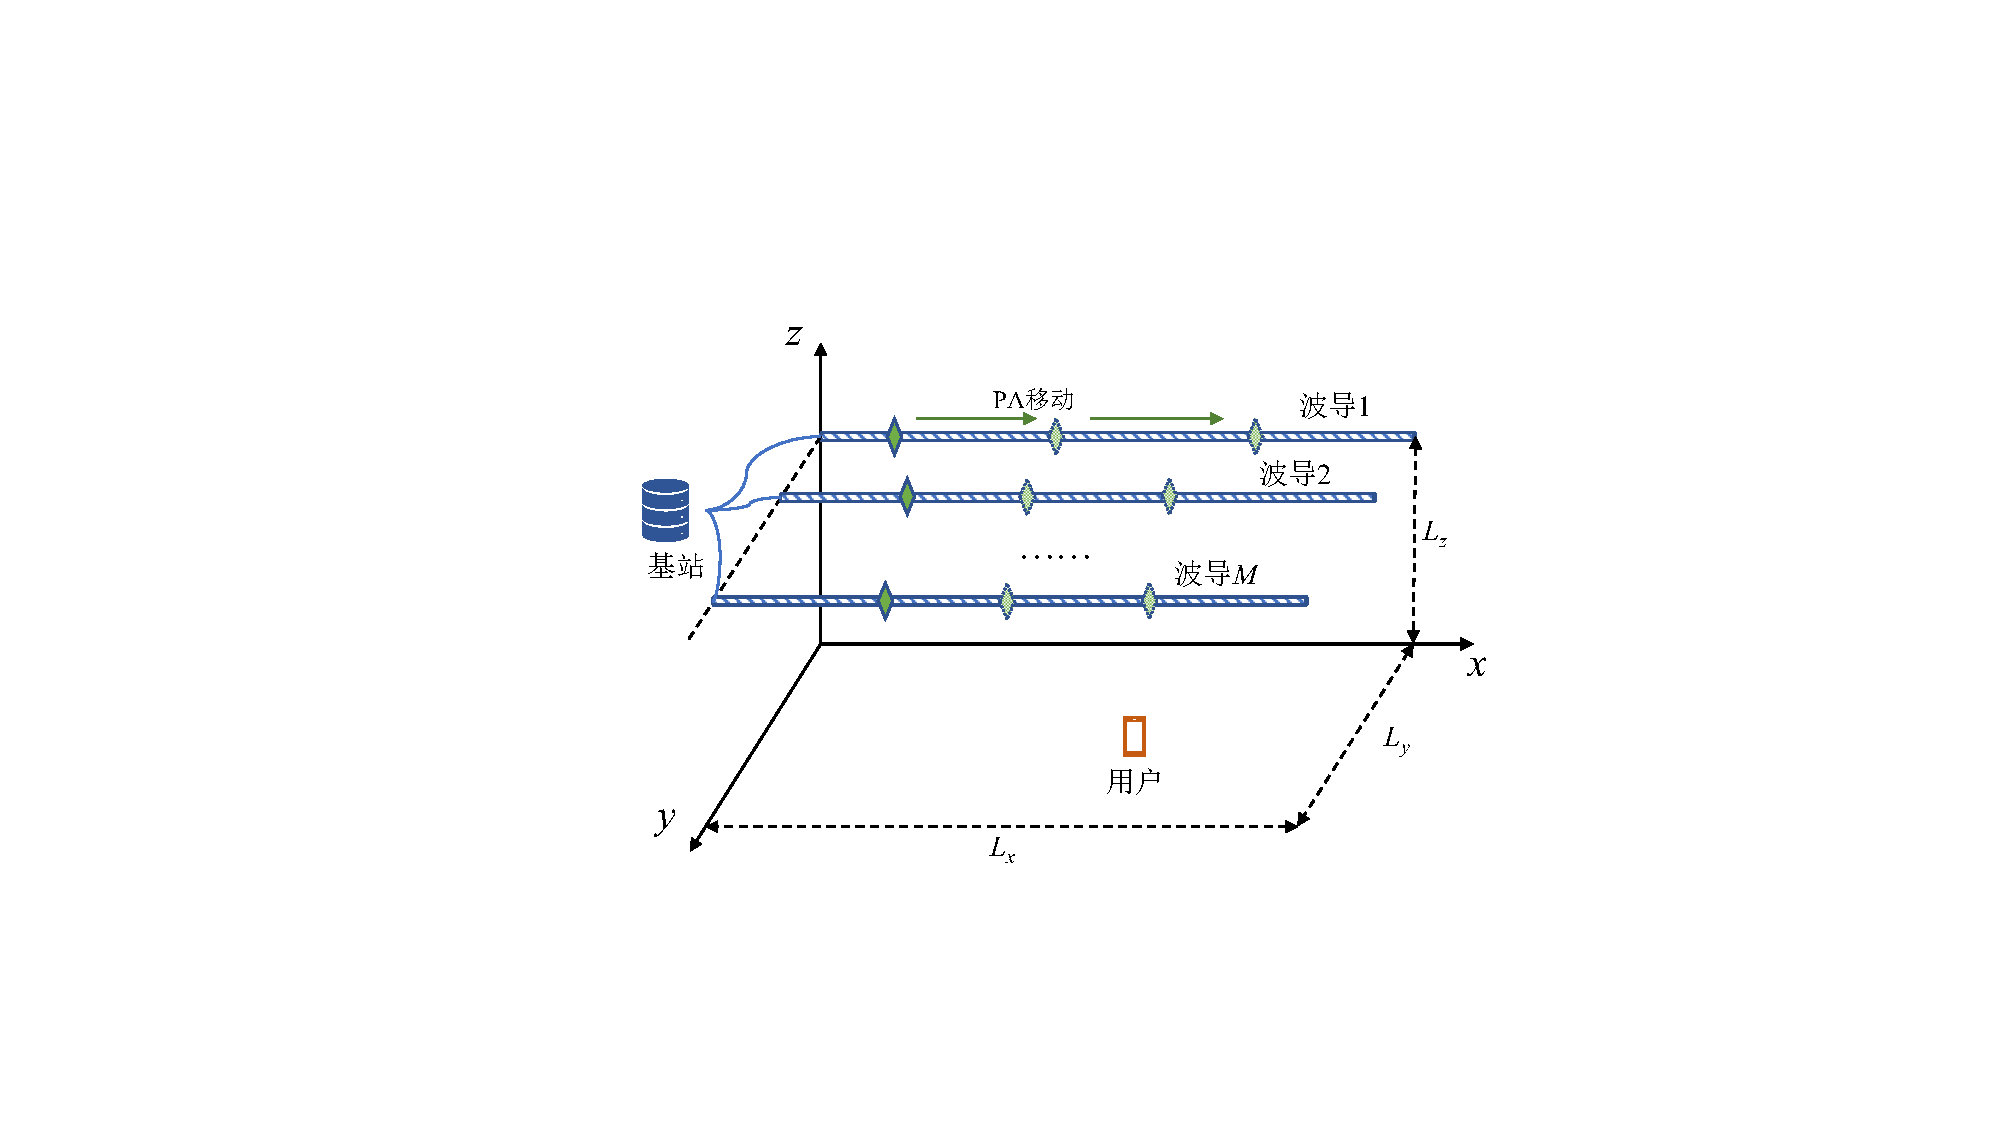
\includegraphics[width=0.6\linewidth]{pass/pass_structure.pdf}
	\caption{捏合天线系统模型}
	\label{fig:pass_structure}
\end{figure}

在捏合天线系统中，用户端到基站端的端到端信道由两段级联而成：其一是从用户到捏合天线的自由空间传播信道；其二是从捏合天线到波导馈电点的波导内部传输信道。
假设用户与捏合天线之间存在视距路径，用户到第$m$个捏合天线的自由空间信道$h_m$可建模为：
\begin{equation}\label{eq:pass_channel_hm}
	h_m = \frac{\sqrt{\eta}}{\|\bm{p}_U - \bm{p}_m\|} e^{-j\frac{2\pi}{\lambda}\|\bm{p}_U - \bm{p}_m\|},
\end{equation}
其中，$\lambda$为自由空间中的载波波长，$\eta = \frac{\lambda^2}{16\pi^2}$为各向同性辐射假设下的参考路径损耗因子，$\|\bm{p}_U - \bm{p}_m\| = \sqrt{(u - x_m)^2 + (v - y_m)^2 + L_z^2}$表示用户与第$m$个捏合天线之间的物理距离。
电磁波被捏合天线耦合进介质波导后，沿着波导向基站馈电点传输。在理想无损波导假设下，电磁波在波导内的传输仅引入额外的相位偏移。因此，第$m$条波导的传输响应函数$g_m$可以表示为：
\begin{equation}\label{eq:pass_channel_gm}
	g_m = e^{-j\frac{2\pi}{\lambda_g} x_m},
\end{equation}
其中，$\lambda_g = \lambda/n_{\mathrm{eff}}$为波导内的导波波长，$n_{\mathrm{eff}}$为波导的有效折射率。

\subsection{上行接收信号模型}

假设用户终端发送的上行数据符号为$s$，满足归一化约束$\mathbb{E}[|s|^2] = 1$，发射功率为$P_t$。则基站端接收到的基带信号向量$\bm{y} \in \mathbb{C}^{M \times 1}$可表示为：
\begin{equation}\label{eq:pass_signal_model}
	\bm{y} = \sqrt{P_t} \bm{G} \bm{h} s + \bm{z},
\end{equation}
其中，$\bm{G} = \mathrm{diag}(g_1, g_2, \cdots, g_M) \in \mathbb{C}^{M \times M}$表示波导传输矩阵，$\bm{h} = [h_1, h_2, \cdots, h_M]^{\mathrm{T}} \in \mathbb{C}^{M \times 1}$表示用户与捏合天线之间的信道向量，$\bm{z} \sim \mathcal{CN}(\bm{0}, \sigma^2 \bm{I}_M)$表示基站接收机引入的加性高斯白噪声，$\sigma^2$为噪声功率。

基站采用最大比合并接收机对多天线信号进行合并处理，以最大化接收信号的信噪比。根据MRC准则，基站端通过对接收信号左乘等效端到端信道的共轭转置来进行相位对齐与信号合并。
定义线性合并向量 $\bm{w} = \bm{G}\bm{h}$，则经过MRC处理后的输出标量信号 $\hat{s}$ 可表示为：
\begin{equation}\label{eq:pass_mrc_signal}
	\hat{s} = \bm{w}^{\mathrm{H}} \bm{y} = (\bm{G}\bm{h})^{\mathrm{H}} (\sqrt{P_t} \bm{G} \bm{h} s + \bm{z}) = \sqrt{P_t}\|\bm{G}\bm{h}\|^2 s + (\bm{G}\bm{h})^{\mathrm{H}} \bm{z}.
\end{equation}

在式~\eqref{eq:pass_mrc_signal}中，有用信号分量的功率为 $P_{\mathrm{sig}} = P_t \|\bm{G}\bm{h}\|^4$，合并后的有效噪声功率为 $P_{\mathrm{noise}} = \mathbb{E}[|(\bm{G}\bm{h})^{\mathrm{H}} \bm{z}|^2] = \sigma^2 \|\bm{G}\bm{h}\|^2$。因此，信噪比可表示为：
\begin{equation}\label{eq:pass_snr_def}
	\mathrm{SNR} = \frac{P_{\mathrm{sig}}}{P_{\mathrm{noise}}} = \frac{P_t \|\bm{G}\bm{h}\|^2}{\sigma^2}.
\end{equation}
由于波导传输矩阵 $\bm{G}$ 为对角阵，且其对角线元素仅包含相位偏转，满足$|g_m| = 1$，说明波导传输过程不会改变信号的能量，即 $\|\bm{G}\bm{h}\|^2 = \|\bm{h}\|^2$。
结合式~\eqref{eq:pass_channel_hm}，系统信噪比可以展开为与所有捏合天线位置$\bm{x} = [x_1, x_2, \cdots, x_M]^{\mathrm{T}}$相关的表达式：
\begin{align}\label{eq:pass_snr_final}
	\mathrm{SNR}(\bm{x}) &= \frac{P_t}{\sigma^2} \|\bm{h}\|^2 
	= \frac{P_t \eta}{\sigma^2} \sum_{m=1}^M \frac{1}{\|\bm{p}_U - \bm{p}_m\|^2} \nonumber \\
	&= \frac{P_t \eta}{\sigma^2} \sum_{m=1}^M \frac{1}{(u - x_m)^2 + (v - y_m)^2 + L_z^2}.
\end{align}

\section{最优天线位置与理论性能分析}

在上一节建立的接收信号模型基础上，本节将首先推导最优天线位置对齐策略及其平均信噪比闭式解，随后基于大阵列渐近，推导PASS系统的空间中断概率。

\subsection{最优对齐策略与平均信噪比推导}

由式~\eqref{eq:pass_snr_final}可知，为了在给定用户位置 $(u, v)$ 的前提下最大化系统通信性能，需要最小化电磁波在自由空间中的大尺度路径损耗。
因此，当且仅当所有捏合天线均滑动至与用户 $x$ 轴坐标对齐时，各天线到用户的欧氏距离达到极小值，即：
\begin{equation}\label{eq:pass_optimal_xm}
	x_m^\ast = u, \quad \forall m \in \{1, 2, \cdots, M\}.
\end{equation}
将式~\eqref{eq:pass_optimal_xm}代入式~\eqref{eq:pass_snr_final}，可得到当前用户位置下的最大信噪比：
\begin{equation}\label{eq:pass_snr_max}
	\mathrm{SNR}_{\max}(v) = \frac{P_t \eta}{\sigma^2} \sum_{m=1}^M \frac{1}{(v - y_m)^2 + L_z^2}.
\end{equation}

上式表明，系统的最大信噪比仅依赖于用户的 $y$ 轴坐标 $v$，而与 $x$ 轴坐标无关。为了进一步评估捏合天线系统在目标覆盖区域内的整体通信能力，下面的定理给出了系统在用户服务平面内的平均信噪比。

\begin{theorem}\label{the:pass_avg_snr}
	假设用户在服务区域$\mathcal{D} = \{ (u,v) \mid 0 \le u \le L_x, 0 \le v \le L_y \}$内服从均匀分布。
	当捏合天线系统采用 $x_m^\ast = u$ 的最优对齐策略时，系统的平均接收信噪比为：
	\begin{equation}\label{eq:pass_avg_snr}
		\overline{\mathrm{SNR}} = \frac{P_t \eta}{\sigma^2 L_y L_z} \sum_{m=1}^M \left[ \arctan\left(\frac{L_y - y_m}{L_z}\right) + \arctan\left(\frac{y_m}{L_z}\right) \right].
	\end{equation}
	进一步地，当系统部署的波导数量 $M$ 较大时，上述平均信噪比可渐近近似为：
	\begin{equation}\label{eq:pass_avg_snr_approx}
		\overline{\mathrm{SNR}} \approx \frac{P_t \eta}{\sigma^2} \left[ \frac{2M-1}{L_y L_z} \arctan\left(\frac{L_y}{L_z}\right) - \frac{M-1}{L_y^2} \ln\left(1 + \frac{L_y^2}{L_z^2}\right) \right].
	\end{equation}
\end{theorem}

\begin{proof}
	由于用户坐标 $(u,v)$ 在区域 $\mathcal{D}$ 内均匀分布，SNR的期望可以表示为：
	\begin{equation}\label{eq:pass_avg_snr_proof_step1}
		\overline{\mathrm{SNR}} = \frac{1}{L_x L_y} \int_0^{L_y} \left( \int_0^{L_x} \mathrm{SNR}_{\max}(v) \, \mathrm{d}u \right) \mathrm{d}v = \frac{P_t \eta}{\sigma^2 L_y} \sum_{m=1}^M \int_0^{L_y} \frac{1}{(v - y_m)^2 + L_z^2} \, \mathrm{d}v.
	\end{equation}
	利用标准积分公式 $\int \frac{1}{x^2 + a^2} \, \mathrm{d}x = \frac{1}{a} \arctan(\frac{x}{a})$，可求得单项的定积分结果为：
	\begin{equation}\label{eq:pass_avg_snr_proof_step2}
		\int_0^{L_y} \frac{1}{(v - y_m)^2 + L_z^2} \, \mathrm{d}v = \frac{1}{L_z} \left[ \arctan\left(\frac{L_y - y_m}{L_z}\right) + \arctan\left(\frac{y_m}{L_z}\right) \right].
	\end{equation}
	将式~\eqref{eq:pass_avg_snr_proof_step2}代回式~\eqref{eq:pass_avg_snr_proof_step1}即可得到式~\eqref{eq:pass_avg_snr}。
	
	当 $M$ 较大时，相邻波导间距 $\Delta y = \frac{L_y}{M-1}$ 较小，令式~\eqref{eq:pass_avg_snr}中的求和项为$g(y) = \arctan(\frac{L_y - y}{L_z}) + \arctan(\frac{y}{L_z})$，根据欧拉–麦克劳林公式的一阶修正，离散求和可近似展开为：
	\begin{equation}\label{eq:pass_avg_snr_proof_step3}
		\sum_{m=1}^M g(y_m) \approx \frac{1}{\Delta y} \int_0^{L_y} g(y) \, \mathrm{d}y + \frac{g(0) + g(L_y)}{2},
	\end{equation}
	其中$g(0) = g(L_y) = \arctan(\frac{L_y}{L_z})$。
	对于连续积分项，利用$g(y)$的对称性，有：
	\begin{equation}\label{eq:pass_avg_snr_proof_step4}
		\int_0^{L_y} g(y) \, \mathrm{d}y = 2 \int_0^{L_y} \arctan\left(\frac{y}{L_z}\right) \mathrm{d}y = 2 \left[ L_y \arctan\left(\frac{L_y}{L_z}\right) - \frac{L_z}{2} \ln\left(1 + \frac{L_y^2}{L_z^2}\right) \right].
	\end{equation}
	将式~\eqref{eq:pass_avg_snr_proof_step3}，式~\eqref{eq:pass_avg_snr_proof_step4}代入式~\eqref{eq:pass_avg_snr}，即可得到式~\eqref{eq:pass_avg_snr_approx}，定理得证。
\end{proof}

定理~\ref{the:pass_avg_snr}从理论上揭示了捏合天线系统通信性能的基本边界与阵列增益特性。由于天线的自适应对齐抵消了$x$轴维度的距离变化，系统的平均信噪比与覆盖区域的长度$L_x$无关。这表明捏合天线系统在长廊、隧道等条状覆盖场景中具有一定的技术优势，相比传统固定基站，能够覆盖远端用户的信号盲区。
渐近解析解~\eqref{eq:pass_avg_snr_approx}剥离了求和算子，表明了在最优对齐策略下，平均信噪比与波导总数$M$呈现线性增长关系，印证了捏合天线系统同样具备阵列增益特性。

\subsection{空间中断概率与通信可靠性分析}

平均信噪比反映了捏合天线系统的整体覆盖能力，但在实际通信系统中，保障处于覆盖区边缘用户的通信可靠性同样至关重要。
为此，引入空间中断概率作为可靠性评估指标，其定义为用户在给定空间中随机分布的情况下，系统瞬时接收信噪比低于预设通信门限 $\gamma_{\mathrm{th}}$ 的概率，即 $P_{\mathrm{out}}(\gamma_{\mathrm{th}}) = \mathrm{Pr}(\mathrm{SNR} < \gamma_{\mathrm{th}})$。
基于前述的大 $M$ 渐近条件，进一步推导出空间中断概率的闭式表达式，如下述命题所示。

\begin{proposition}\label{pro:pass_outage_prob}
	假设用户在服务区域$\mathcal{D} = \{ (u,v) \mid 0 \le u \le L_x, 0 \le v \le L_y \}$内服从均匀分布。
	在天线数量$M$较大的渐近条件下，系统的空间中断概率为：
	\begin{equation}\label{eq:pass_outage_prob}
		P_{\mathrm{out}}(\gamma_{\mathrm{th}}) =
		\begin{cases}
			0, & \gamma_{\mathrm{th}} \le \gamma_{\min}, \\
			1 - \sqrt{1 - 4\left(\frac{L_z}{L_y}\right)^2 + \frac{4L_z}{L_y}\cot\left(\frac{\gamma_{\mathrm{th}}}{C}\right)}, & \gamma_{\min} < \gamma_{\mathrm{th}} < \gamma_{\max}, \\
			1, & \gamma_{\mathrm{th}} \ge \gamma_{\max},
		\end{cases}
	\end{equation}
	其中，常数$C = \frac{P_t \eta (M-1)}{\sigma^2 L_y L_z}$，$\gamma_{\min} = C \arctan\left(\frac{L_y}{L_z}\right)$，$\gamma_{\max} = 2C \arctan\left(\frac{L_y}{2L_z}\right)$。
\end{proposition}

\begin{proof}
	由式~\eqref{eq:pass_snr_max}可知，系统的最大信噪比仅取决于用户的纵坐标$v$，在波导数量$M$较大的条件下，连续渐近下的SNR可表示为：
	\begin{align}\label{eq:pass_snr_v_approx}
		\mathrm{SNR}(v) &\approx \frac{P_t \eta}{\sigma^2} \frac{M-1}{L_y} \int_0^{L_y} \frac{1}{(v - y)^2 + L_z^2} \,\mathrm{d}y \nonumber \\
		&= C \left[ \arctan\left(\frac{v}{L_z}\right) + \arctan\left(\frac{L_y - v}{L_z}\right) \right].
	\end{align}
	对$\mathrm{SNR}(v)$关于$v$求导，可得：
	\begin{equation}
		\frac{\mathrm{d}(\mathrm{SNR}(v))}{\mathrm{d}v} = C \left[ \frac{1/L_z}{1 + (v/L_z)^2} - \frac{1/L_z}{1 + ((L_y - v)/L_z)^2} \right].
	\end{equation}
	令导数为0，有：$v^2 = (L_y - v)^2$，解得区间$[0, L_y]$内的唯一驻点为$v = L_y/2$。
	通过单调性分析可知，$\mathrm{SNR}(v)$在区间$[0, L_y/2]$上单调递增，在$[L_y/2, L_y]$上单调递减，且关于中心线$v = L_y/2$呈轴对称分布。
	因此，信噪比的边界值为最小值$\gamma_{\min} = \mathrm{SNR}(0) = C \arctan\left(\frac{L_y}{L_z}\right)$，中心值为最大值$\gamma_{\max} = \mathrm{SNR}(L_y/2) = 2C \arctan\left(\frac{L_y}{2L_z}\right)$。
	
	根据空间中断概率的定义可知，当 $\gamma_{\mathrm{th}} \le \gamma_{\min}$ 时，全区域满足通信要求，无中断发生；当 $\gamma_{\mathrm{th}} \ge \gamma_{\max}$ 时，全区域均无法满足要求，通信完全中断。
	当 $\gamma_{\min} < \gamma_{\mathrm{th}} < \gamma_{\max}$ 时，中断发生在靠近端点的两个边缘区域，即$v \in [0, v_1) \cup (v_2, L_y]$，$v_1,v_2$是方程$\mathrm{SNR}(v) = \gamma_{\mathrm{th}}$的根。对方程两边同时取正切，利用正切函数的和角公式可得：
	\begin{equation}
		\tan\left(\frac{\gamma_{\mathrm{th}}}{C}\right) = \frac{\frac{v}{L_z} + \frac{L_y - v}{L_z}}{1 - \frac{v(L_y - v)}{L_z^2}} = \frac{L_y L_z}{L_z^2 - L_y v + v^2}.
	\end{equation}
	整理可得关于$v$的一元二次方程：
	\begin{equation}
		v^2 - L_y v + L_z^2 - L_y L_z \cot\left(\frac{\gamma_{\mathrm{th}}}{C}\right) = 0.
	\end{equation}
	根据一元二次方程求根公式，覆盖达标区域的长度为：
	\begin{equation}
		\Delta v = v_2 - v_1 = \sqrt{L_y^2 - 4L_z^2 + 4L_y L_z \cot(\frac{\gamma_{\mathrm{th}}}{C})}.
	\end{equation}
	则中断概率为中断区间长度与总长度的比$P_{\mathrm{out}}(\gamma_{\mathrm{th}}) = \frac{L_y - \Delta v}{L_y}$，将 $\Delta v$ 代入即得式~\eqref{eq:pass_outage_prob}。命题得证。
\end{proof}

命题~\ref{pro:pass_outage_prob}说明当用户位于边缘区域时，由于远端波导上的天线到用户的传播距离增加，导致系统容易在边缘处发生通信中断。
为了保证边缘用户的服务质量，除了增加发射功率外，增加波导部署密度也是降低中断概率的直接途径，在实际PASS系统应综合服务区域面积和信噪比要求来确定部署的波导数量。

\section{基于圆形几何的交替天线配置与定位算法}

上一节的分析表明，当捏合天线系统用于通信传输时，最优的天线配置策略是将所有捏合天线动态滑动并对齐至用户的横坐标。
这说明基站准确获取用户的位置坐标是执行动态波束赋形和提升通信性能的前提。
然而，在实际的通信场景中，用户位置往往是未知的信息，需要依靠接收到的上行导频信号进行估计。
如果PASS系统采用固定的天线几何构型，例如使用通信最优的共线排布进行位置估计，会使得空间分集缺失，从而难以提供高精度的定位结果。
因此，为了精准获取用户位置以支撑后续的波束赋形，同时挖掘PASS系统在定位感知方面的潜力，本节将利用捏合天线位置的动态可重构特性，重塑空间传播几何构型，提出一种联合用户位置估计与天线几何配置的优化框架。

\subsection{基于FIM的定位问题建模}

为了实现高精度的用户定位并优化天线配置，首先需要在初始天线状态下获取用户位置的粗估计。随后，对位置估计的理论误差下界进行分析，建立位置估计误差最小化的天线放置问题。

在给定的初始天线配置下，基站可以通过经典的二维多重信号分类算法对用户的平面坐标 $\bm{p}_U = [u, v, 0]^{\mathrm{T}}$ 进行初步估计\cite{schmidt1986multiple}。
假设用户在 $T$ 个连续快拍内发送导频序列 $\bm{s} = [s_1, s_2, \cdots, s_T]^{\mathrm{T}} \in \mathbb{C}^{T \times 1}$，根据前文建立的式~\eqref{eq:pass_signal_model}，基站端接收到的信号矩阵 $\bm{Y} = [\bm{y}_1, \bm{y}_2, \cdots, \bm{y}_T] \in \mathbb{C}^{M \times T}$ 可表示为：
\begin{equation}\label{eq:pass_music_Y}
	\bm{Y} = \sqrt{P_t} \bm{G} \bm{h} \bm{s}^{\mathrm{T}} + \bm{Z},
\end{equation}
其中，$\bm{Z} = [\bm{z}_1, \bm{z}_2, \cdots, \bm{z}_T] \in \mathbb{C}^{M \times T}$ 为加性高斯白噪声矩阵。
接收信号的样本协方差矩阵可计算为：
\begin{equation}\label{eq:pass_music_R}
	\hat{\bm{R}} = \frac{1}{T} \bm{Y} \bm{Y}^{\mathrm{H}}.
\end{equation}

对协方差矩阵 $\hat{\bm{R}}$ 进行奇异值分解，将其划分为信号子空间与噪声子空间：
\begin{equation}\label{eq:pass_music_svd}
	\hat{\bm{R}} = \bm{w}_s \Lambda_s \bm{w}_s^{\mathrm{H}} + \bm{W}_z \bm{\Lambda}_z \bm{W}_z^{\mathrm{H}},
\end{equation}
其中，信号子空间由对应最大奇异值$\Lambda_s$的左奇异列向量 $\bm{w}_s \in \mathbb{C}^{M \times 1}$ 构成；$\bm{W}_z \in \mathbb{C}^{M \times (M-1)}$ 为对应其余 $(M-1)$ 个较小奇异值的左奇异矩阵，代表噪声子空间；$\bm{\Lambda}_z \in \mathbb{R}^{(M-1) \times (M-1)}$ 为包含这些噪声奇异值的对角矩阵。

定义潜在用户位置 $(u,v)$ 对应的阵列导向矢量为 $\bm{a}(u,v) \triangleq \bm{G} \bm{h}(u,v)$。根据 MUSIC 算法的正交性原理，真实用户位置 $(\bar{u}, \bar{v})$ 对应的导向矢量位于信号子空间内，因而与噪声子空间正交，即 $\bm{W}_z^{\mathrm{H}} \bm{a}(\bar{u}, \bar{v}) = \bm{0}$。因此，可构造二维MUSIC空间谱函数如下：
\begin{equation}\label{eq:pass_music_spectrum}
	P_{\mathrm{MUSIC}}(u,v) = \frac{1}{\bm{a}^{\mathrm{H}}(u,v)\bm{W}_z \bm{W}_z^{\mathrm{H}}\bm{a}(u,v)}.
\end{equation}
通过在目标服务区域内搜索空间谱的谱峰，即可获得用户位置的估计$(\hat{u}, \hat{v})$：
\begin{equation}\label{eq:pass_music_peak}
	(\hat{u}, \hat{v}) = \mathop{\arg\max}_{u \in [0,L_x], v \in [0,L_y]} P_{\mathrm{MUSIC}}(u,v).
\end{equation}

上式的估计精度受限于当前固定的天线几何位置。因此，将天线位置 $\bm{x} = [x_1, x_2, \cdots, x_M]^{\mathrm{T}}$ 作为可调优化的变量，进一步改善传播几何结构，是提升定位精度的关键。在复高斯观测模型下，任意无偏估计量对用户位置 $(u,v)$ 的估计性能受限于克拉美-罗下界。具体而言，二维位置估计的均方误差满足以下不等式：
\begin{equation}\label{eq:pass_mse_crlb}
	\mathrm{MSE}(u,v) = \mathbb{E}\left[ (u-\hat{u})^2+(v-\hat{v})^2 \right] \geq \mathrm{tr}\left( \bm{J}^{-1}(u, v) \right),
\end{equation}
其中，$\bm{J}(u, v) \in \mathbb{R}^{2 \times 2}$ 为费雪信息矩阵。

依据式~\eqref{eq:pass_signal_model}的系统模型，可知接收信号$\bm{y} \sim \mathcal{CN}(\bm{\mu}(u,v), \sigma^2 \bm{I}_M)$，其中，均值向量为$\bm{\mu}(u,v) = \sqrt{P_t} \bm{G} \bm{h}(u,v) s$。
FIM 的第$(i,j)$个元素可由均值向量对参量的偏导数内积求得：
\begin{equation}\label{eq:pass_slepian_bangs}
	[\bm{J}]_{i,j} = \frac{2}{\sigma^2} \Re \left\{ \left( \frac{\partial \bm{\mu}}{\partial \theta_i} \right)^{\mathrm{H}} \left( \frac{\partial \bm{\mu}}{\partial \theta_j} \right) \right\}, \quad i, j \in \{1, 2\},
\end{equation}
其中$\theta_1 = u,\, \theta_2 = v$。
由于波导传输矩阵 $\bm{G}$ 是仅包含相位信息的对角阵，且不依赖于用户坐标 $(u,v)$，因此满足酉矩阵性质 $\bm{G}^{\mathrm{H}}\bm{G} = \bm{I}_M$。在计算偏导数时，$\bm{G}$ 的影响被抵消，例如对于横坐标$u$，有：
\begin{equation}\label{eq:pass_fim_deriv}
	\left( \frac{\partial \bm{\mu}}{\partial u} \right)^{\mathrm{H}} \left( \frac{\partial \bm{\mu}}{\partial u} \right) = P_t |s|^2 \left( \frac{\partial \bm{h}}{\partial u} \right)^{\mathrm{H}} \bm{G}^{\mathrm{H}} \bm{G} \left( \frac{\partial \bm{h}}{\partial u} \right) = P_t \left\| \frac{\partial \bm{h}}{\partial u} \right\|^2,
\end{equation}
其中，$\frac{\partial \bm{h}}{\partial u}$ 和 $\frac{\partial \bm{h}}{\partial v}$ 分别表示用户与捏合天线之间的信道向量相对于用户二维坐标的梯度。
同理可求得其他的偏导数项，将所有项代入式~\eqref{eq:pass_slepian_bangs}中，得到FIM的表达式：
\begin{equation}\label{eq:pass_fim_matrix}
	\bm{J}(u,v) = \frac{2 P_t}{\sigma^2} \,
	\Re \left\{
	\begin{bmatrix}
		\left\| \frac{\partial \bm{h}}{\partial u} \right\|^2 & \left( \frac{\partial \bm{h}}{\partial u} \right)^{\mathrm{H}} \frac{\partial \bm{h}}{\partial v} \\
		\left( \frac{\partial \bm{h}}{\partial v} \right)^{\mathrm{H}} \frac{\partial \bm{h}}{\partial u} & \left\| \frac{\partial \bm{h}}{\partial v} \right\|^2
	\end{bmatrix}
	\right\}.
\end{equation}

从式~\eqref{eq:pass_fim_matrix}中可以看出，FIM中的梯度项仅依赖于信道$\bm{h}$，受天线位置坐标$\bm{x}$的影响。为了最大化接收信号中所蕴含的位置信息，实现定位误差下界的最小化，可以通过调整天线位置 $\bm{x}$ 来最小化 FIM 逆矩阵的迹。由此，可建立如下的天线位置优化问题：
\begin{equation}\label{eq:pass_prob_p1}
	\begin{aligned}
		\min_{\bm{x}} \quad & \mathrm{tr}\left( \bm{J}^{-1}(\bm{x}, u, v) \right), \\
		\text{s.t.} \quad & 0 \leq x_m \leq L_x, \quad m = 1, 2, \cdots, M.
	\end{aligned}
\end{equation}

优化问题~\eqref{eq:pass_prob_p1}准确地刻画了最小化定位误差下界的理论准则。然而，由于对FIM的求逆操作引入了非线性的强耦合项，各个捏合天线坐标 $x_m$ 之间相互依赖，问题高度非凸，需要通过复杂的优化方法解决，不存在闭式表达式。接下来的小节将对该目标函数进行合理的松弛与推导，以揭示定位导向的最优几何分布形态。

\subsection{定位导向的最优天线几何形态}

为了获得具有物理意义且计算高效的天线几何分布策略，本节引入空间感知中经典的“各向同性误差”假设对问题进行合理松弛化。
从几何角度看，当缺乏某一方向的观测信息时，该方向的误差将急剧放大并主导总误差，呈现出狭长的误差椭圆。
因此，最优的捏合天线分布会自然地倾向于从各个正交方向均衡地获取目标信息，在目标周围形成具有高度空间对称性的均匀观测视角，使误差椭圆向正圆收敛。
在此状态下，$x$轴与$y$轴方向的估计误差方差相近且相关性较弱，故两个正交方向的费雪信息近似相等，即$J_{uu} \approx J_{vv} \triangleq J_0$，交叉耦合项$J_{uv}$趋近于0，可以近似忽略FIM的非对角线元素。
将上述近似条件代入原目标函数，可得：
\begin{equation}\label{eq:pass_trJ_inv_approx}
	\mathrm{tr}(\bm{J}^{-1}) = \frac{J_{uu} + J_{vv}}{J_{uu}J_{vv} - J_{uv}^2} \approx \frac{2J_0}{J_0^2 - 0} = \frac{2}{J_0}.
\end{equation}
同时，FIM 的迹可表示为 $\mathrm{tr}(\bm{J}) = J_{uu} + J_{vv} \approx 2J_0$。由此可见，最小化$\mathrm{tr}(\bm{J}^{-1})$与最大化 $\mathrm{tr}(\bm{J})$具有一致性。
从特征值角度看，设FIM的两个正特征值为$\alpha_1$ 与 $\alpha_2$，根据均值不等式，有：
\begin{equation}
	\mathrm{tr}(\bm{J})\,\mathrm{tr}(\bm{J}^{-1}) =
	(\alpha_1 + \alpha_2)(\alpha_1^{-1} + \alpha_2^{-1})\ge 4,
\end{equation}
在各向同性假设下，$\alpha_1=\alpha_2$，不等式取等，同样证明了一致性。
因此，采用最大化FIM的迹$\mathrm{tr}(\bm{J})$作为替代准则，不仅解除了天线位置变量间的非线性耦合，有效降低了优化复杂度，而且通常能够得到高质量的近似解。替代的优化问题表示如下：
\begin{equation}\label{eq:pass_prob_p2}
	\begin{aligned}
		\max_{\bm{x}} \quad & \mathrm{tr}\left( \bm{J}(\bm{x}, u, v) \right), \\
		\text{s.t.} \quad & 0 \leq x_m \leq L_x, \quad m = 1, 2, \cdots, M.
	\end{aligned}
\end{equation}

针对优化问题~\eqref{eq:pass_prob_p2}，若暂时忽略边界约束，目标函数中蕴含着极具物理指导意义的结构特征。下面的定理给出了能够最大化总体费舍尔信息的最优天线几何分布规律。

\begin{theorem}\label{the:pass_optimal_geometry}
	在天线可于 $z = L_z$ 平面内任意部署的无约束条件下，优化问题~\eqref{eq:pass_prob_p2} 的最优解为：所有捏合天线均分布在一个以目标用户正上方点 $(u, v, L_z)$ 为圆心的圆周上，且该最优圆周的半径为：
	\begin{equation}\label{eq:pass_optimal_radius}
		r^\ast = \sqrt{
			\frac{
				- \lambda^2 
				+ \sqrt{ \lambda^4 + 4\pi^2 \lambda^2 L_z^2 + 16\pi^4 L_z^4 }
			}{
				4\pi^2
		}}.
	\end{equation}
\end{theorem}

\begin{proof}
	根据式~\eqref{eq:pass_fim_matrix}，费雪信息矩阵的迹可以展开为：
	\begin{equation}\label{eq:pass_trJ_expand}
		\mathrm{tr}(\bm{J}) = \frac{2P_t}{\sigma^2} \sum_{m=1}^{M} \left( \left| \frac{\partial h_m}{\partial u} \right|^2 + \left| \frac{\partial h_m}{\partial v} \right|^2 \right),
	\end{equation}
	其中$h_m = \sqrt{\eta} d_m^{-1} e^{-j\frac{2\pi}{\lambda} d_m}$，$d_m = \|\bm{p}_U - \bm{p}_m\|$。
	
	对 $h_m$ 关于横坐标 $u$ 求偏导可得：
	\begin{equation}\label{eq:pass_hm_deriv_u}
		\frac{\partial h_m}{\partial u} = h_m \left( -\frac{1}{d_m} - j \frac{2\pi}{\lambda} \right) \frac{\partial d_m}{\partial u}, \quad \text{其中} \quad \frac{\partial d_m}{\partial u} = \frac{u - x_m}{d_m}.
	\end{equation}
	计算关于$u$的偏导数的模平方，可得：
	\begin{equation}\label{eq:pass_hm_deriv_u_sq}
		\left| \frac{\partial h_m}{\partial u} \right|^2 = \eta \frac{(u-x_m)^2}{d_m^6} \left(1 + \frac{4\pi^2 d_m^2}{\lambda^2}\right).
	\end{equation}
	同理，对纵坐标 $v$ 的偏导数的模平方为：
	\begin{equation}\label{eq:pass_hm_deriv_v_sq}
		\left| \frac{\partial h_m}{\partial v} \right|^2 = \eta \frac{(v-y_m)^2}{d_m^6} \left(1 + \frac{4\pi^2 d_m^2}{\lambda^2}\right).
	\end{equation}
	
	将式~\eqref{eq:pass_hm_deriv_u_sq}与式~\eqref{eq:pass_hm_deriv_v_sq}代入式~\eqref{eq:pass_trJ_expand}，并利用几何关系 $(u-x_m)^2 + (v-y_m)^2 = d_m^2 - L_z^2$，可将 $\mathrm{tr}(\bm{J})$ 化简为关于距离 $d_m$ 的函数：
	\begin{equation}\label{eq:pass_trJ_final}
		\mathrm{tr}(\bm{J}) = \frac{2P_t \eta}{\sigma^2} \sum_{m=1}^M \left(1 + \frac{4\pi^2 d_m^2}{\lambda^2}\right) \left(\frac{1}{d_m^4} - \frac{L_z^2}{d_m^6}\right).
	\end{equation}
	
	式~\eqref{eq:pass_trJ_final}表明，最大化迹的目标函数可以完全解耦为$M$个独立子问题。忽略常数项，定义单个天线对目标函数的贡献函数为 $f(d)$，有：
	\begin{equation}\label{eq:pass_func_d}
		f(d) = \left(1 + \frac{4\pi^2 d^2}{\lambda^2}\right) \left(\frac{1}{d^4} - \frac{L_z^2}{d^6}\right),\, d \ge L_z.
	\end{equation}
	对 $f(d)$ 关于 $d$ 求导：
	\begin{equation}\label{eq:pass_func_d_deriv}
		f'(d) = \frac{1}{d^7} \left( -4d^2 + 6L_z^2 - \frac{8\pi^2}{\lambda^2} d^4 + \frac{16\pi^2 L_z^2}{\lambda^2} d^2 \right).
	\end{equation}
	令 $f'(d) = 0$，可将其转化为关于 $d^2$ 的一元二次方程：
	\begin{equation}\label{eq:pass_d_quadratic}
		4\pi^2 (d^2)^2 + (2\lambda^2 - 8\pi^2 L_z^2) d^2 - 3\lambda^2 L_z^2 = 0.
	\end{equation}
	求解该方程并舍去负根，可得到最优距离$d^\ast$：
	\begin{equation}\label{eq:pass_d_ast}
		d^\ast = \sqrt{ \frac{ (4\pi^2 L_z^2 - \lambda^2) + \sqrt{ (\lambda^2 - 4\pi^2 L_z^2)^2 + 12\pi^2 \lambda^2 L_z^2 } }{4\pi^2} }.
	\end{equation}
	由于所有捏合天线均被约束在高度为 $L_z$ 的平面内，其对应的最优水平投影半径为 $r^\ast = \sqrt{(d^\ast)^2 - L_z^2}$。将式~\eqref{eq:pass_d_ast}代入并化简，即可得到式~\eqref{eq:pass_optimal_radius}，定理得证。
\end{proof}

定理~\ref{the:pass_optimal_geometry}给出了最大化$\mathrm{tr}(\bm{J})$的最优半径表达式。在实际的微波或毫米波频段PASS系统中，由于工作波长通常远小于波导安装高度，上述表达式可以进一步简化，如下面的推论所示。

\begin{corollary}\label{cor:pass_high_freq}
	当系统满足高频近似条件 $L_z \gg \lambda$ 时，最优圆形阵列的半径可简化为：
	\begin{equation}\label{eq:pass_r_ast_approx}
		r^\ast \approx L_z - \frac{\lambda^2}{16\pi^2 L_z} \approx L_z.
	\end{equation}
\end{corollary}

\begin{proof}
	定义$\varepsilon = \lambda/L_z \ll 1$。提取式~\eqref{eq:pass_optimal_radius}最内层根号中的 $16\pi^4 L_z^4$ 作为公因式，内部的二次根号项可以写为：
	\begin{equation}
		\sqrt{ \lambda^4 + 4\pi^2 \lambda^2 L_z^2 + 16\pi^4 L_z^4 } = 4\pi^2 L_z^2 \sqrt{ 1 + \frac{\varepsilon^2}{4\pi^2} + \frac{\varepsilon^4}{16\pi^4} }.
	\end{equation}
	忽略高阶小量$\varepsilon^4/(16\pi^4)$，并利用一阶泰勒展开式 $\sqrt{1+x} \approx 1 + x/2$，该项可近似为：
	\begin{equation}
		4\pi^2 L_z^2 \left( 1 + \frac{\varepsilon^2}{8\pi^2} \right) = 4\pi^2 L_z^2 + \frac{1}{2}\lambda^2.
	\end{equation}

	将上述近似结果代回式~\eqref{eq:pass_optimal_radius}中化简，由于 $\frac{\lambda^2}{8\pi^2 L_z^2} \ll 1$，对最外层根号再次运用一阶泰勒展开 $\sqrt{1-x} \approx 1 - x/2$，可得：
	\begin{equation}
		r^\ast \approx \sqrt{ \frac{-\lambda^2 + 4\pi^2 L_z^2 + \frac{1}{2}\lambda^2}{4\pi^2} } = L_z \sqrt{ 1 - \frac{\lambda^2}{8\pi^2 L_z^2} } \approx L_z \left( 1 - \frac{\lambda^2}{16\pi^2 L_z^2} \right) \approx L_z.
	\end{equation}
	推论得证。
\end{proof}

推论~\ref{cor:pass_high_freq}为确定理想的天线圆排布提供了一条直观的准则：最优捏合天线半径等于波导的部署高度。
考虑到实际中天线只能沿着特定的波导滑动，通过将理想圆周上的点投影至最近的可行域边界内，可计算出实际可行的第$m$个捏合天线目标位置：
\begin{equation}\label{eq:pass_xm_clip}
	x_m^\ast = 
	\begin{cases}
		\mathop{\mathrm{clip}}\limits_{[0,\,L_x]}\!\left( u \pm \sqrt{(r^\ast)^2 - (v - y_m)^2} \right), & r^\ast > |v - y_m|, \\
		u, & \text{其它},
	\end{cases}
\end{equation}
其中，操作符 $\mathrm{clip}(\cdot)$ 用于将坐标截断，约束在波导的物理长度 $[0, L_x]$ 内。对于穿过目标圆的波导，在实际排布中可以交替分配正负号以确保天线阵列的几何对称性，进一步减弱 $u$ 和 $v$ 两个维度的估计误差之间的耦合。

对比本节基于定位感知的最优圆形分布与上一节基于通信传输的最优共线分布，揭示了捏合天线系统中通信与感知功能之间的内在矛盾：将所有捏合天线对齐于用户正上方能够最大化阵列接收增益与通信信噪比，但这种共线的构型会引起严重的几何精度衰减，导致定位精度较差；相反，最优定位要求天线分散部署于特定的圆环轨迹上以构建丰富的多视角观测，但这不可避免地增加了大尺度路径损耗，降低了通信速率。

\subsection{CG-APPL算法设计}

结合前文建立的二维MUSIC定位估计方法与基于费雪信息最大化的天线几何配置策略，本小节提出一种基于圆形几何的交替天线配置与定位算法。该算法通过交替迭代的方式，逐步优化用户位置估计与捏合天线的几何分布，其核心思想如下：首先利用初始的天线阵列构型获取用户位置的粗估计；随后，根据该估计位置计算最优的观测圆半径，并驱动捏合天线向理想的圆形几何分布滑动以重构阵列；在新构型下，能够获取包含更高费雪信息的观测数据，从而在后续迭代中实现更高精度的位置估计。

随着上述交替迭代过程的不断深入，天线构型逐渐逼近用户正上方的最优圆周，定位误差稳步收敛。当两次相邻迭代间的用户估计位置变化量低于预设的阈值，或达到最大迭代次数 $I$ 时，算法终止。
CG-APPL算法的完整执行流程总结于算法~\ref{alg:pass_cg_appl}中。

\begin{algorithm}[!htbp]
	\caption{基于圆形几何的交替天线配置与定位算法（CG-APPL）}
	\label{alg:pass_cg_appl}
	\begin{algorithmic}[1]
		\REQUIRE 初始天线位置向量 $\bm{x}^{(1)}$，最大迭代次数 $I$。
		\ENSURE 最终的用户位置估计 $(\hat{u}, \hat{v})$。
		\FOR{$i = 1, 2, \cdots, I$}
		\STATE \textbf{// 步骤 1：位置估计更新}
		\STATE 在当前天线配置 $\bm{x}^{(i)}$ 下获取接收导频信号矩阵 $\bm{Y}^{(i)}$；
		\STATE 根据式~\eqref{eq:pass_music_R}计算样本协方差矩阵 $\hat{\bm{R}}$，并按式~\eqref{eq:pass_music_svd}进行奇异值分解；
		\STATE 求解式~\eqref{eq:pass_music_peak}，通过二维空间谱搜索获得当前用户位置估计 $(\hat{u}^{(i)}, \hat{v}^{(i)})$；
		\STATE \textbf{// 步骤 2：天线位置更新}
		\STATE 依据式~\eqref{eq:pass_optimal_radius}或高频近似式~\eqref{eq:pass_r_ast_approx}计算最优半径 $(r^\ast)^{(i)}$；
		\STATE 根据投影映射公式~\eqref{eq:pass_xm_clip}交替分配符号，更新各捏合天线位置$\bm{x}^{(i+1)}$；
		\STATE \textbf{若} $\|(\hat{u}^{(i)}, \hat{v}^{(i)}) - (\hat{u}^{(i-1)}, \hat{v}^{(i-1)})\|_2$ 小于预设阈值 \textbf{则} 提前终止迭代；
		\ENDFOR
		\RETURN 最终用户位置估计 $(\hat{u}, \hat{v}) = (\hat{u}^{(I)}, \hat{v}^{(I)})$。
	\end{algorithmic}
\end{algorithm}


\section{数值仿真分析}

本节通过蒙特卡洛仿真，验证本章所提的捏合天线通信理论性能分析结果以及CG-APPL算法的有效性。本节首先介绍系统的默认参数设置与对比基准方案；随后，验证不同波导部署数量下的平均信噪比与空间中断概率的理论解；最后，深入分析所提定位算法在不同导频开销、发射功率、空间几何条件下的定位精度。
%，并揭示捏合天线系统在通信与感知功能之间的性能折中关系。


\subsection{仿真参数设置与基准方案}

为了贴近实际的室内捏合天线部署场景，本节设定目标服务区域$\mathcal{D}$的长、宽分别为 $L_x = 10 \text{ m}$ 与 $L_y = 10 \text{ m}$，捏合波导水平悬挂于 $L_z = 3 \text{ m}$ 的天花板高度。系统默认部署波导数量为 $M = 10$，均匀分布在 $y$ 轴方向上。
系统工作于典型的微波频段，载波频率设定为 $f_c = 1 \text{ GHz}$。在此工作频率下，波导高度 $L_z$ 远大于波长 $\lambda$，满足$L_z \gg \lambda$的高频近似条件。
在提出的联合定位算法中，二维 MUSIC 空间谱的峰值搜索采用“粗-精”两阶段搜索策略，不仅消除了粗网格量化带来的误差，还降低了搜索的复杂度。
除非在具体仿真中另有说明，本节的所有数值仿真均采用表~\ref{tab:pass_sim_params}中列出的默认参数，且所有结果均通过$N_{\mathrm{mc}}$次蒙特卡洛随机试验取平均得到，每次试验中的用户位置在服务区域$\mathcal{D}$内随机生成。

\begin{table}[!htbp]
	\centering
	\caption{捏合天线系统仿真参数表}
	\label{tab:pass_sim_params}
	\begin{tabular}{cc}
		\toprule
		\textbf{参数} & \textbf{数值} \\
		\midrule
		服务区域长度 $L_x$ / 宽度 $L_y$ & $10 \text{ m}$ / $10 \text{ m}$ \\
		波导部署高度 $L_z$ & $3 \text{ m}$ \\
		捏合波导 / 天线数量 $M$ & $10$ \\
		载波频率 $f_c$ & $1 \text{ GHz}$ \\
		用户发射功率 $P_t$ & $30 \text{ dBm}$ \\
		噪声功率 $\sigma^2$ & $-30 \text{ dBm}$ \\
		导频序列快拍数 $T$ & $20$ \\
		二维MUSIC粗搜 / 精搜步长 & $0.1 \text{ m}$ / $0.001 \text{ m}$ \\
		CG-APPL迭代次数 $I$ & $3$ \\
		蒙特卡洛试验次数 $N_{\mathrm{mc}}$ & $320$ \\
		\bottomrule
	\end{tabular}
\end{table}

本节引入以下三种定位基准方案与所提CG-APPL算法进行对比分析：
\begin{itemize}
	\item \textbf{WLS方案：}
	该方案中，所有捏合天线固定在波导的起始端（即 $x_m = 0, \forall m$），不进行滑动调整。基站基于该固定构型接收到的信号，采用基于接收信号强度的加权最小二乘算法进行位置估计\cite{zhang2025pinchingantenna}。

	\item \textbf{MUSIC方案：}
	天线配置与WLS方案相同，但在位置估计环节，采用本章提出的二维MUSIC谱峰搜索算法。该方案用于评估在相同固定几何构型下，高分辨率子空间算法相对于传统WLS算法的性能提升。
	
	\item \textbf{WLS-AO方案：}
	该方案保留了本章提出的动态天线配置策略，但在每次迭代更新天线位置后，采用WLS算法重新估计用户位置。该方案旨在验证最优圆形分布策略对不同定位估计算法的普适增强效果。
\end{itemize}

本节采用二维均方根误差（Root Mean Squared Error，RMSE）对定位精度进行评价，其定义为：
\begin{equation}\label{eq:pass_rmse_def}
	\mathrm{RMSE} = \sqrt{ \frac{1}{N_{\mathrm{mc}}} \sum_{n=1}^{N_{\mathrm{mc}}} \left[ (u_n - \hat{u}_n)^2 + (v_n - \hat{v}_n)^2 \right] },
\end{equation}
其中 $(u_n, v_n)$ 和 $(\hat{u}_n, \hat{v}_n)$ 分别表示第 $n$ 次蒙特卡洛试验中的真实用户坐标与估计用户坐标。


\subsection{捏合天线通信理论性能验证}

本小节主要验证捏合天线系统通信性能的理论推导，包括定理~\ref{the:pass_avg_snr}中的平均信噪比与命题~\ref{pro:pass_outage_prob}中的空间中断概率。

\begin{figure}[!htbp]
	\centering
	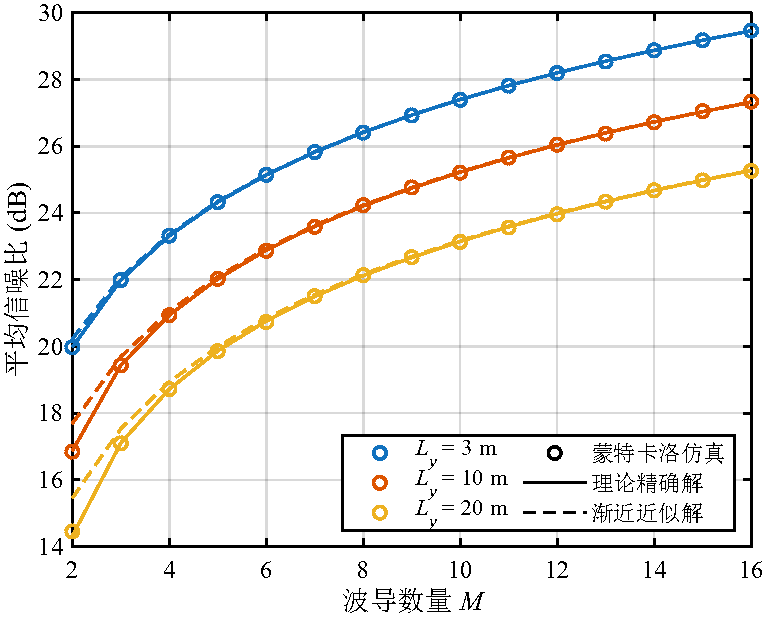
\includegraphics[width=0.6\linewidth]{pass/pass_figSNRvsM.pdf}
	\caption{不同区域宽度$L_y$下，平均信噪比与波导数量$M$的关系}
	\label{fig:pass_figSNRvsM}
\end{figure}

图~\ref{fig:pass_figSNRvsM} 给出了在不同服务区域宽度（$L_y = 3 \text{ m}, 10 \text{ m}, 20 \text{ m}$）下，系统平均接收信噪比随部署波导数量 $M$ 的变化曲线。
从图中可以观察到，在所有区域宽度下，蒙特卡洛仿真结果与式~\eqref{eq:pass_avg_snr}给出的理论精确解完全吻合，对于式~\eqref{eq:pass_avg_snr_approx}所给出的渐近近似解，在波导数量较少时，由于相邻波导间距较大，会引入微小误差；然而随着$M$增大，该渐近解迅速收敛至精确解，说明所推导的近似表达式在较大波导数量条件下具有很好的适用性。此外，在固定 $M$ 的情况下，服务区域宽度 $L_y$ 的增大会导致平均信噪比下降，其原因是区域越宽，用户分布于远离阵列中心的边缘区域的概率越高，从而使得大尺度路径损耗的平均值上升。

\begin{figure}[!htbp]
	\centering
	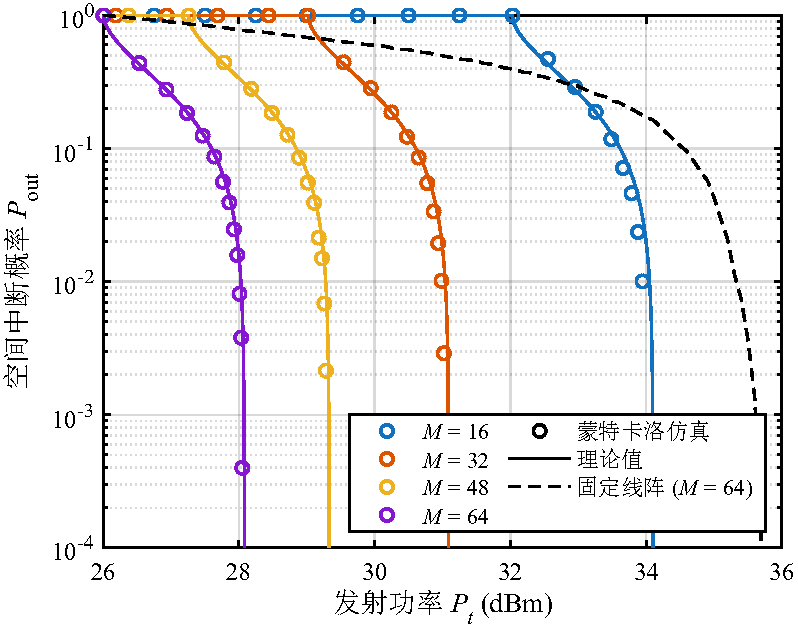
\includegraphics[width=0.6\linewidth]{pass/pass_figOutagevsPt.pdf}
	\caption{不同波导数量$M$下，空间中断概率随发射功率的变化曲线}
	\label{fig:pass_figOutagevsPt}
\end{figure}

图~\ref{fig:pass_figOutagevsPt} 展示了在目标通信信噪比门限为$\gamma_{\text{th}}=30$~dB的条件下，系统空间中断概率 $P_{\mathrm{out}}$ 随用户发射功率 $P_t$ 的变化曲线，并对比了不同波导部署密度（$M = 16, 32, 48, 64$）下的性能。同时，图中引入了天线在起始端且规模为$M=64$的传统固定线阵作为对比基准。
从图中可以看出，捏合天线系统相较于同等规模的传统固定线阵展现出了压倒性的优势，在相同的中断概率下所需的发射功率显著降低。这一优势主要源于捏合天线的可移动特性，有效缩短了信号传播距离，抑制大尺度的路径损耗，并维持稳定的LoS链路。相比之下，传统固定天线对边缘用户的覆盖较差，导致其中断概率曲线随发射功率增加下降缓慢。
例如，为达到$10^{-3}$的中断概率，固定线阵需要超过 $35.5\ \text{dBm}$ 的发射功率，比捏合天线系统高出约 $7.5\ \text{dB}$。
此外，随着波导数量的增加，中断性能逐渐改善，曲线整体左移。
例如，为保证 $10^{-3}$ 的中断概率，当$M$ 从 $16$ 增至 $64$ 时，所需发射功率由约 $34\ \text{dBm}$ 下降至约 $28\ \text{dBm}$。
最后，图中所有配置下的蒙特卡洛仿真结果均与理论曲线吻合良好，尤其在中断概率急剧下降的“瀑布区”表现一致，从而验证了命题~\ref{pro:pass_outage_prob}所推导的表达式。



\subsection{联合定位与天线配置算法性能分析}

本小节将全面评估CG-APPL算法的综合性能。通过分析天线构型与空间谱的动态演变过程、不同系统参数对定位RMSE的影响，并结合全区域RMSE热力图，探讨动态几何重构对定位精度的提升作用。

\begin{figure}[!htbp]
	\centering
	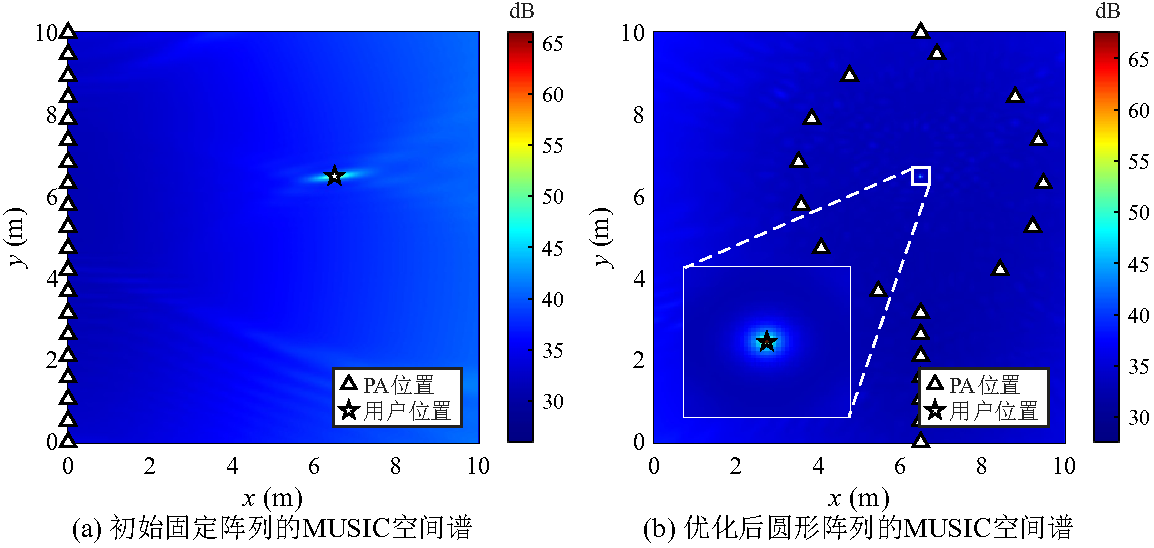
\includegraphics[width=0.85\linewidth]{pass/pass_figMUSICheatmap.pdf}
	\caption{天线几何构型演变与 MUSIC 空间谱对比}
	\label{fig:pass_figMUSICheatmap}
\end{figure}

图~\ref{fig:pass_figMUSICheatmap}展示了捏合天线系统在优化前后的阵列几何形态以及对应的二维MUSIC空间谱图。图中仿真采用 $M=20$ 条波导的密集配置，以清晰呈现阵列构型的变化，目标用户位于$(6.5, 6.5) \text{ m}$处。
如图~\ref{fig:pass_figMUSICheatmap}(a)所示，在初始阶段，传统的固定线阵虽然能够通过MUSIC算法估计出用户的大致位置，但其空间谱峰较为平缓，且存在明显径向拖尾。这种观测不对称在图中表现为狭长的误差椭圆，从而制约了定位精度。
而图~\ref{fig:pass_figMUSICheatmap}(b)经过重构阵列形态，形成了一个以目标为中心、半径约为$L_z$的离散对称圆形阵列。在此几何构型下，阵列可从正交方向均匀地获取目标的空间信息，空间谱的谱峰因此变得尖锐集中。这一结果表明，圆形几何构型有效克服了单侧观测的局限，有效提升了系统的空间分辨率与定位精度。

\begin{figure}[!htbp]
	\centering
	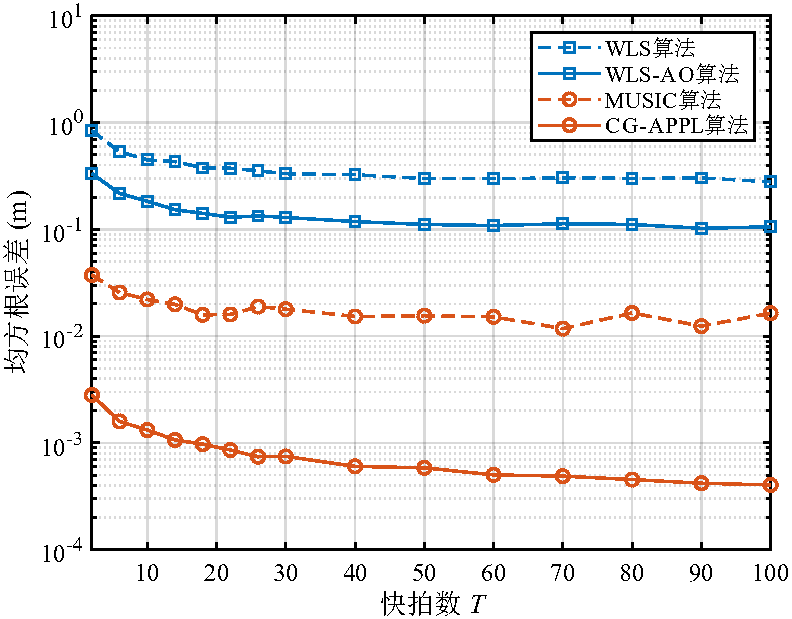
\includegraphics[width=0.6\linewidth]{pass/pass_figRMSEvsNT.pdf}
	\caption{不同算法的定位均方根误差随导频快拍数 $T$ 的变化曲线}
	\label{fig:pass_figRMSEvsNT}
\end{figure}

在明确了圆形几何构型对空间分辨率的提升效果后，系统实际部署中的导频资源分配问题也需要重点考量。导频序列过短会使得噪声无法被充分平均，增大定位误差；而导频序列过长又会占用过多的通信资源，并引入不必要的定位时延。
图~\ref{fig:pass_figRMSEvsNT} 展示了在发射功率 $P_t = 30 \text{ dBm}$、噪声功率为 $-35 \text{ dBm}$ 的条件下，四种算法的RMSE随导频快拍数 $T$的变化关系。
从图中可以看出：在 $T$ 较小的阶段，所有算法的RMSE均随快拍数增加而迅速下降；当 $T > 20$ 后，各算法的误差曲线逐渐趋于平缓。WLS与MUSIC算法的误差在达到一定下限后基本不再改善，CG-APPL算法虽在 $T$ 继续增加时仍有微小精度提升，但边际收益已不明显。
综合以上分析，将导频快拍数设定为$T = 20$是一种兼顾精度与开销的工程折中方案。在此条件下，CG-APPL能实现毫米级精度的定位，本节的后续仿真均采用 $T = 20$这一快拍数。

\begin{figure}[!htbp]
	\centering
	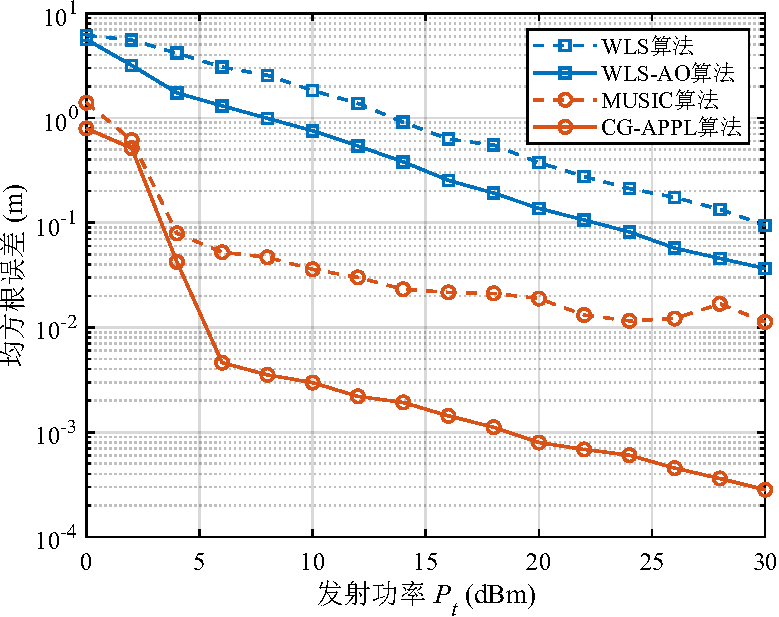
\includegraphics[width=0.6\linewidth]{pass/pass_figRMSEvsTransmitPower.pdf}
	\caption{不同算法的定位均方根误差随发射功率的变化曲线}
	\label{fig:pass_figRMSEvsTransmitPower}
\end{figure}

图~\ref{fig:pass_figRMSEvsTransmitPower} 展示了在噪声功率固定为 $-45 \text{ dBm}$ 的条件下，四种定位算法的均方根误差随目标用户发射功率 $P_t$ 的变化关系。
从图中可以看出，所有算法的 RMSE 均随 $P_t$ 的增加而下降，这是高信噪比条件下信号分量增强、噪声影响减弱的直接体现。
然而，不同算法的性能差距十分显著：一方面，基于固定线阵的二维 MUSIC 算法凭借其高分辨谱峰提取能力，在整个功率范围内均优于基于能量检测的固定 WLS 算法；另一方面，引入阵列重构策略的 WLS-AO 与本章提出的 CG-APPL 算法，其精度均显著超越对应的固定线阵算法。
在低发射功率的阶段，当有效信号刚刚从强噪声背景中浮现时，CG-APPL 算法的误差曲线呈现急剧下降；进入高发射功率段后，其通过粗‑精两阶段搜索克服了离散网格误差，RMSE 继续保持下降趋势，并与 WLS-AO 的下降趋势一致，最终达到亚毫米级的定位精度。

\begin{figure}[!htbp]
	\centering
	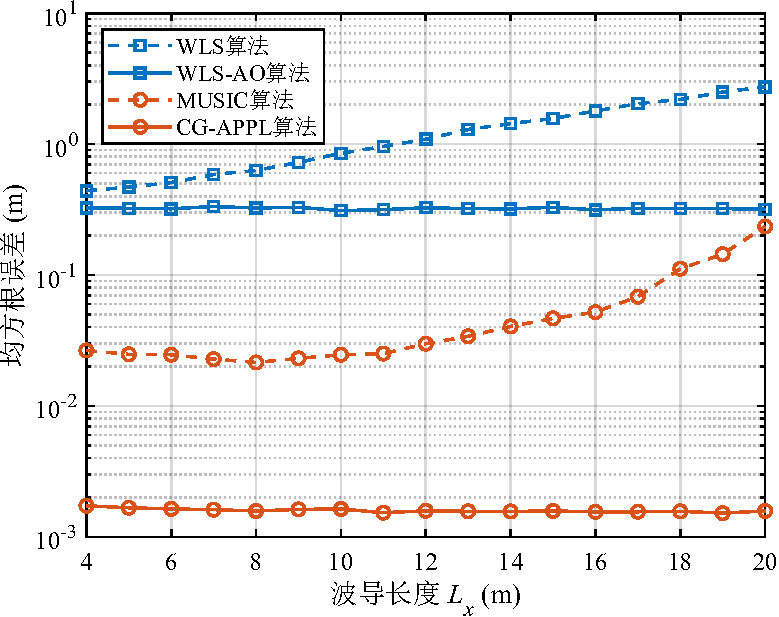
\includegraphics[width=0.6\linewidth]{pass/pass_figRMSEvsLx.pdf}
	\caption{不同定位算法的均方根误差随波导长度 $L_x$ 的变化曲线}
	\label{fig:pass_figRMSEvsLx}
\end{figure}

为了探究服务区域尺寸对系统定位鲁棒性的影响，图~\ref{fig:pass_figRMSEvsLx} 给出了在噪声功率为 $-30 \text{ dBm}$ 的条件下，四种算法的定位均方根误差随 $x$ 轴方向的房间深度 $L_x$ 的变化情况。仿真中 $L_x$ 由 $4 \text{ m}$ 逐步增至 $20 \text{ m}$，目标用户在各尺寸区域内服从随机均匀分布。
整体来看，随着波导长度增加，用户可能的分布范围扩大，远端用户路径损耗增大，导致固定观测视角下几何精度衰减。这使得固定天线阵列方案的定位误差持续上升，而具备动态重构能力的算法则表现出几乎不受房间深度影响的稳定性能。
进一步对比这两种动态方案，本章所提的 CG-APPL 算法凭借子空间高分辨率搜索，其 RMSE 在整个 $L_x$ 变化范围内始终稳定在 $10^{-3} \text{ m}$ 量级，优于基于信号强度的 WLS-AO 算法。


\begin{figure}[!htbp]
	\centering
	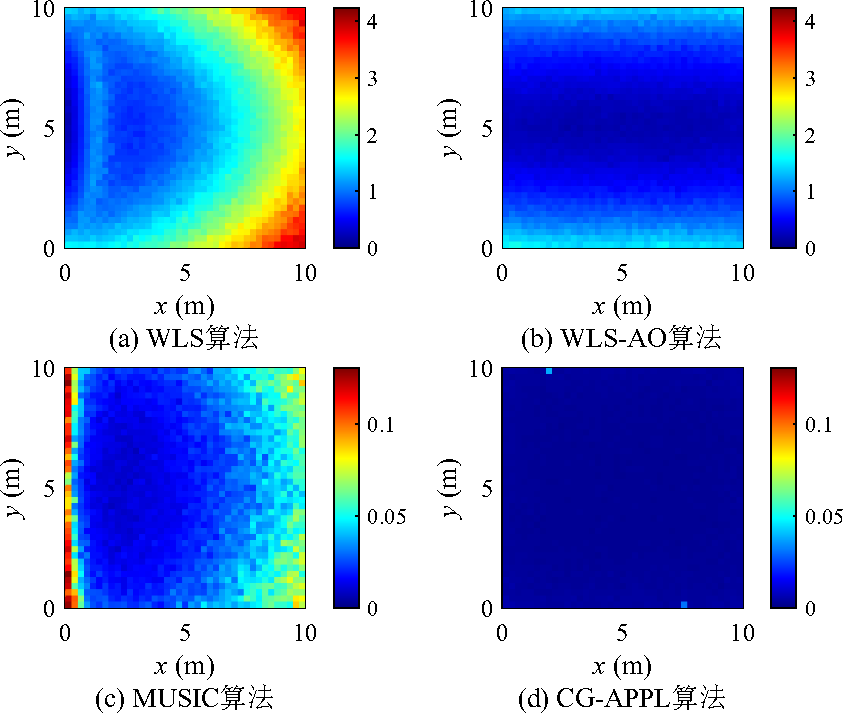
\includegraphics[width=0.6\linewidth]{pass/pass_figRMSEheatmap.pdf}
	\caption{噪声功率为 $-25 \text{ dBm}$ 条件下，四种算法的全区域定位 RMSE 空间热力图}
	\label{fig:pass_figRMSEheatmap_cn}
\end{figure}

图~\ref{fig:pass_figRMSEheatmap_cn} 展示了在噪声功率为 $-25 \text{ dBm}$ 时，四种算法的定位性能在全服务区域内的空间分布细节。仿真中将 $10 \text{ m} \times 10 \text{ m}$ 的房间离散为 $40 \times 40$ 的网格，热力图中每个单元的颜色代表用户落入该区域时的平均 RMSE。
从热力图的空间分布可见，基于初始固定阵列的 WLS 与 MUSIC 算法，其误差在空间上的分布较为不均匀。随着目标远离阵列，尤其在房间深处与角落，路径损耗增大，观测信噪比恶化，形成深红色的高误差区。
值得注意的是，图~\ref{fig:pass_figRMSEheatmap_cn}(c)显示固定 MUSIC 算法虽然在远端误差较低，但在紧邻 $y$ 轴的区域却出现了一条红色误差带，其误差甚至高于远端。这印证了前文理论分析的观点：当用户极度靠近并与固定阵列近似共线时，观测视角失去几何多样性，导致沿法线方向的分辨能力丧失。
相比之下，采用自适应阵列重构的方案则表现出优秀的全局均匀性。
图~\ref{fig:pass_figRMSEheatmap_cn}(b) 显示 WLS-AO 算法有效缓解了房间角落的误差上升。
从图~\ref{fig:pass_figRMSEheatmap_cn}(d) 可以看出，CG-APPL 算法消除了全区域内的高误差盲区，整幅热力图呈现均匀的深蓝色。
这一结果表明，基于几何引导的动态天线重构不仅能有效提升定位准确度，更是实现室内全域无缝高精度感知的重要基础。





\section{本章小结}


\noindent\rule{\linewidth}{2pt}

\textcolor{red}{之后再写}

\chapter{可重构智能表面自适应波束赋形算法与原型系统实测}\label{ch:ris}

\section{引言}

\textcolor{red}{内容构思：简述RIS在6G中的重要地位（低功耗、低成本重塑信道）。点出现有大量RIS波束赋形算法依赖理想信道状态信息（CSI），但在实际原型系统中，信道估计开销巨大且硬件仅支持离散（如1-bit）相移。引出本章的动机：设计不依赖显式CSI估计、基于接收功率反馈的实用型自适应波束赋形算法（GFB与ASG），并自主研制大规模RIS原型系统，通过仿真与多场景实测验证其性能。}

\section{系统模型}

本章考虑一个由可重构智能表面辅助的单输入单输出下行无线通信系统。如图~\ref{fig:ris_structure}所示，该系统包含一个配备单天线的基站、一个单天线用户，以及在两者之间部署的 RIS。该 RIS 由 $N$ 个无源反射单元构成，并连接一个智能控制器。控制器一方面可调节各反射单元的相移，另一方面能够通过专用有线或无线通信链路，接收来自用户端的参考信号接收功率反馈信息。

\begin{figure}[!htbp]
	\centering
	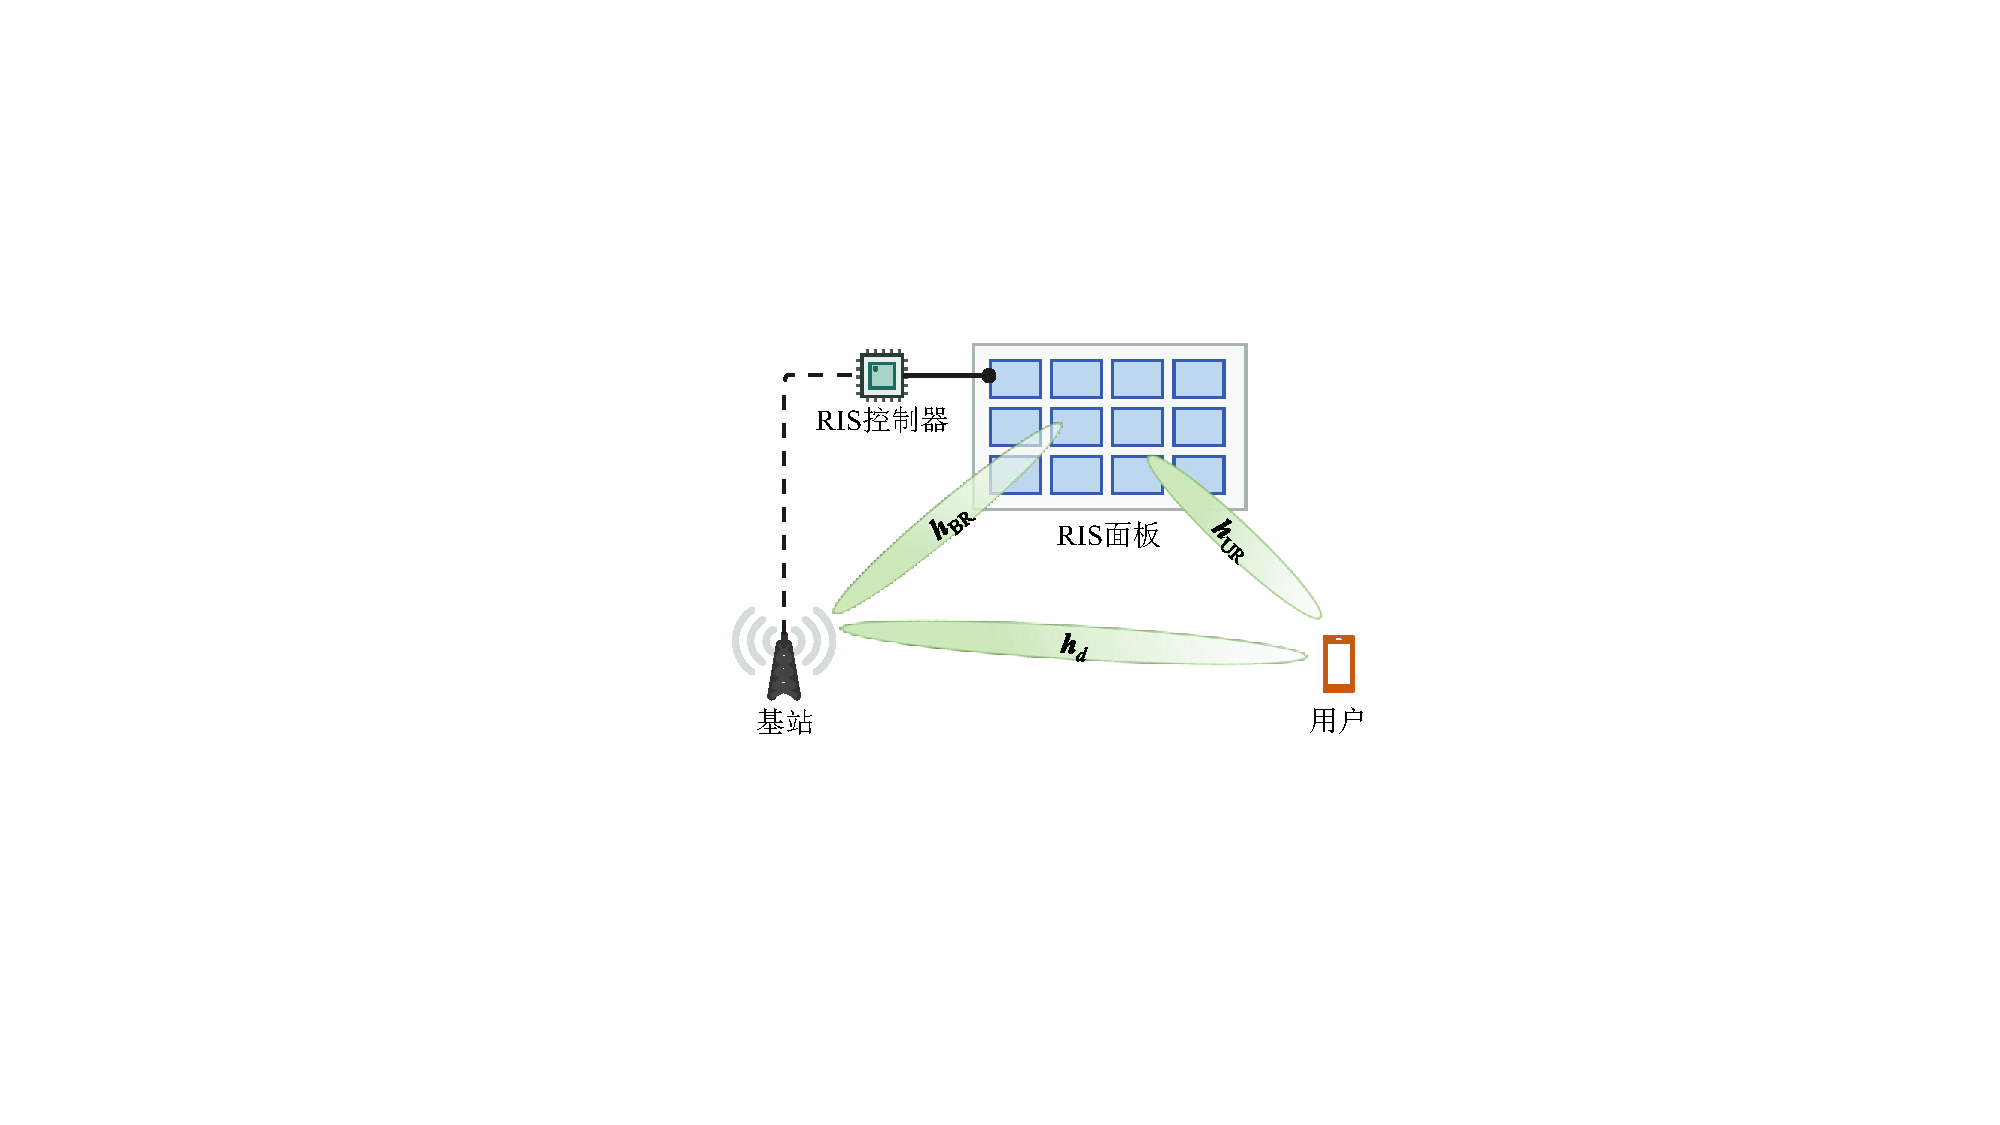
\includegraphics[width=0.5\linewidth]{ris/ris_structure.pdf}
	\caption{RIS 辅助的下行无线通信系统模型}
	\label{fig:ris_structure}
\end{figure}

假设系统处于典型的低速移动场景，信道表现为窄带准静态衰落。根据图~\ref{fig:ris_structure}，令 $h_d \in \mathbb{C}$ 表示基站到用户的直射信道，$\bm{h}_\mathrm{BR} \in \mathbb{C}^{N \times 1}$ 和 $\bm{h}_\mathrm{UR} \in \mathbb{C}^{N \times 1}$ 分别表示从基站到 RIS，以及从 RIS到用户的信道向量。定义 RIS 面板的反射系数向量为 $\bm{\phi} = [\phi_1, \dots, \phi_N]^T \in \mathbb{C}^{N \times 1}$，其中 $\phi_n = e^{j\theta_n}$ 为第 $n$ 个反射单元的反射系数，$\theta_n$ 为对应的相移。考虑到实际硬件的控制精度，相移 $\theta_n$ 通常被限制在一个离散的有限集合中取值。假设每个相移由 $b$ 比特进行均匀量化，则其可取的离散值间隔为 $\Delta\theta = 2\pi / 2^b$。

为简化表达，定义 $\bm{h}_r \in \mathbb{C}^{N \times 1}$ 为基站经由 RIS 到达用户的等效级联信道，即 $\bm{h}_r = \text{diag}(\bm{h}_\mathrm{UR})\bm{h}_\mathrm{BR}$。此时，基站到用户的信道由直射路径与级联反射路径叠加而成，用户端接收到的基带信号 $y$ 可表示为：
\begin{equation}
	y = \sqrt{P_t} (h_d + \bm{h}_r^\mathrm{T} \bm{\phi}) s + z,
\end{equation}
其中，$P_t$ 为基站发射功率，$s$ 是满足 $\mathbb{E}[|s|^2] = 1$ 的发送符号，$z \sim \mathcal{CN}(0, \sigma^2)$ 为加性复高斯噪声。
于是，用户端解码数据符号 $s$ 的信噪比可由 RIS 的反射系数向量 $\bm{\phi}$ 决定，可写为：
\begin{equation}\label{eq:ris_snr_definition}
	\text{SNR}(\bm{\phi}) = \frac{P_t |h_d + \bm{h}_r^\mathrm{T} \bm{\phi}|^2}{\sigma^2}.
\end{equation}

RIS系统的目标是通过联合设计所有反射单元的离散相移，寻找最优的反射系数向量$\bm{\phi}$，以最大化式~\eqref{eq:ris_snr_definition}所定义的接收信噪比。该优化问题可建模为：
\begin{equation}\label{eq:ris_optimization_problem}
	\begin{aligned}
		\max_{\bm{\phi}} \quad & \frac{P_t |h_d + \bm{h}_r^\mathrm{T} \bm{\phi}|^2}{\sigma^2}, \\
		\text{s.t.} \quad & \phi_n = e^{j\theta_n}, \quad \forall n = 1, \dots, N, \\
		& \theta_n \in \left\{ 0, \Delta\theta, 2\Delta\theta, \dots, (2^b - 1)\Delta\theta \right\}.
	\end{aligned}
\end{equation}

直接求解该优化问题的前提是需要准确地获取全局的精确信道状态信息$h_d$和$\bm{h}_r$。然而，由于 RIS 通常由无源器件构成，不配备射频链路和基带信号处理模块，它无法像常规基站设备那样主动收发导频信号来辅助信道估计。
若要在基站或用户端估计等效级联信道 $\bm{h}_r$，需要设计特定的导频传输与 RIS 反射模式。
由于级联信道维度与反射单元数量 $N$ 成正比，为区分每个 $h_{r,n}$ 的贡献，所需的导频开销至少与 $N$ 呈线性关系，当 $N$ 很大时，会造成相当大的系统开销；同时，单个级联反射信道强度远弱于背景信道，估计时也容易产生较大误差。
此外，传统的基于导频的信道估计方法需要对现有无线通信协议进行修改，以支持基站、RIS 和用户之间的指令交互与协作测量，阻碍了RIS的快速灵活部署。

为克服上述困难，本章研究无需显式获取 CSI 的盲波束赋形方法，利用用户端易于获取的参考信号接收功率作为优化的依据。由于测量过程不可避免地包含噪声，用户端测得的 RSRP 的期望值可表示为信号功率与噪声功率之和：
\begin{equation}\label{eq:ris_rsrp_definition}
	\mathbb{E}\left[\text{RSRP}(\bm{\phi})\right] = \mathbb{E}\left[|y|^2\right] = P_t \left| h_d + \bm{h}_r^\mathrm{T} \bm{\phi} \right|^2 + \sigma^2.
\end{equation}
对比发现，最大化 RSRP 在数学上与最大化 SNR 是完全等价的。于是，RIS 控制器可以周期性地调整其反射配置 $\bm{\phi}$，并根据用户反馈的 RSRP 来评估该配置的优劣，进而迭代地搜索最优解，实现在线优化。这一策略无需修改现有通信协议，具有良好的工程可实现性。下一节将针对这一问题模型，提出基于分组反馈的波束赋形算法，以在有限的反馈开销下高效地寻找最优的 RIS 配置。


\section{基于接收功率反馈的自适应波束赋形算法}


如上一节所述，将 RIS 的相移优化转化为最大化 RSRP 的盲优化问题，避开了较为困难的信道状态信息获取环节。然而，由式~\eqref{eq:ris_optimization_problem}可知，若直接在整个离散可行域内进行穷举搜索，其解空间大小高达 $(2^b)^N$。对于包含数百上千个反射单元的 RIS 面板而言，在实际系统较短的信道相干时间内无法穷举。因此，本节将提出两种启发式的自适应波束赋形算法。


\subsection{快速贪婪波束赋形算法}


在视距占主导或仅存在单一强多径的典型通信场景中，最优的 RIS 反射相移在空间分布上往往具有高度的结构化特征。
假设总数为 $N$ 的 RIS 反射单元呈均匀平面阵列排列，包含 $N_z$ 行与 $N_y$ 列，且行列天线间距分别为 $d_z$ 与 $d_y$。
采用标准的 3GPP 空间坐标系建模，假设 RIS 面板垂直放置（位于 $y$-$z$ 平面），在远场平面波假设下，任意空间方向 $(\vartheta, \varphi)$ 对应的阵列导向矢量 $\bm{a}(\vartheta, \varphi) \in \mathbb{C}^{N \times 1}$ 可表示为水平和垂直两个均匀线阵导向矢量的克罗内克积：
\begin{equation}
	\bm{a}(\vartheta, \varphi) = \bm{a}_y(\vartheta, \varphi) \otimes \bm{a}_z(\vartheta),
\end{equation}
其中$\bm{a}_y(\vartheta, \varphi) \in \mathbb{C}^{N_y \times 1}$ 和 $\bm{a}_z(\vartheta) \in \mathbb{C}^{N_z \times 1}$ 分别表示沿$y$ 轴水平与$z$ 轴垂直的一维导向矢量，其表达式如下：
\begin{align}
	\bm{a}_y(\vartheta, \varphi) &= \left[ 1, e^{-j\frac{2\pi}{\lambda} d_y \sin\vartheta \sin\varphi}, \dots, e^{-j\frac{2\pi}{\lambda} d_y (N_y-1) \sin\vartheta \sin\varphi} \right]^\mathrm{T}, \\
	\bm{a}_z(\vartheta) &= \left[ 1, e^{-j\frac{2\pi}{\lambda} d_z \cos\vartheta}, \dots, e^{-j\frac{2\pi}{\lambda} d_z (N_z-1) \cos\vartheta} \right]^\mathrm{T},
\end{align}
其中 $\vartheta$ 和 $\varphi$ 分别表示空间中的天顶角与方位角，$\lambda$ 为载波波长。

设基站到 RIS 的到达角为 $(\vartheta_t, \varphi_t)$，RIS 到用户的出发角为 $(\vartheta_r, \varphi_r)$。若要最大化端到端的接收信号功率，在连续相移条件下，最优的 RIS 反射系数向量 $\bm{\phi}_{\text{opt}}$ 应当使各级联路径的信号在接收端相位完全对齐，即满足：
\begin{equation}\label{eq:ris_opt_continuous_phi}
	\bm{\phi}_{\text{opt}} = \left( \bm{a}(\vartheta_r, \varphi_r) \odot \bm{a}(\vartheta_t, \varphi_t) \right)^*,
\end{equation}
其中 $\odot$ 表示哈达玛积。于是，理想的最优相移向量可以分解为列维度和行维度复指数矢量的克罗内克积。
当阵列规模较大时，这类具有等差相位梯度的导向矢量可以用离散傅里叶变换（Discrete Fourier Transform，DFT）矩阵的列向量高精度地近似\cite{yin2013coordinated,adhikary2013joint}。具体而言，定义维度为 $K \times K$ 的标准 DFT 矩阵 $\mathcal{F}(K)$ 如下：
\begin{equation}
	\mathcal{F}(K) = \begin{bmatrix}
		1 & 1 & 1 & \cdots & 1 \\
		1 & \xi & \xi^{2} & \cdots & \xi^{K-1} \\
		1 & \xi^{2} & \xi^{2 \cdot 2} & \cdots & \xi^{2(K-1)} \\
		\vdots & \vdots & \vdots & \ddots & \vdots \\
		1 & \xi^{K-1} & \xi^{2(K-1)} & \cdots & \xi^{(K-1)(K-1)}
	\end{bmatrix},
\end{equation}
其中，复指数项 $\xi = e^{-j(2\pi/K)}$表示相邻单元间的空间相位差。


基于此，对于 $N_z \times N_y$ 的平面阵列，RIS 的波束赋形码本可构建为 $\mathcal{F}(N_y) \otimes \mathcal{F}(N_z)$。该码本矩阵中的每一列，都对应着物理空间中一个特定的反射波束指向。这说明在连续相移空间中，最优的 RIS 表面相位分布呈现出沿行列方向的二维线性渐变；然而，当受限于低分辨率的离散量化，在物理空间上处于同一行或同一列的相邻反射单元有一定概率具有完全相同的相移状态。

快速贪婪波束赋形算法正是受此二维DFT码本空间量化特性的启发。为压缩搜索空间，GFB 放弃了对单个反射单元的独立盲搜，转而利用阵列的行列几何结构进行降维。为便于直观表述，将原一维反射系数向量 $\bm{\phi}$ 重新映射为反应二维物理位置的矩阵 $\bm{\Phi} \in \mathbb{C}^{N_z \times N_y}$。GFB 算法通过按行或按列对相移进行 $180^\circ$的整体翻转来执行局部搜索，整个算法分为水平搜索与垂直搜索两个连续阶段。算法首先以一个全部相同相位的初始矩阵启动，并记录初始的 RSRP 测量值。随后，逐列或逐行生成探测矩阵并下发至 RIS 面板。若探测状态下的 RSRP 较历史最佳值有所提升，则保留该翻转操作并更新最佳状态；反之，则拒绝翻转，恢复至上一状态。


\begin{algorithm}[!htbp]
	\caption{快速贪婪波束赋形算法（GFB）}
	\label{alg:ris_gfb}
	\begin{algorithmic}[1]
		\REQUIRE RIS 面板行数 $N_z$ 与列数 $N_y$，接收端实时反馈的RSRP测量值 $P(\cdot)$。
		\ENSURE 优化后的 RIS 二维反射系数矩阵 $\bm{\Phi}_{\text{GFB}}$。
		
		\STATE \textbf{// 步骤 1：系统初始化}
		\STATE 生成全 $1$ 的初始反射系数矩阵 $\bm{\Phi}_{0} \in \mathbb{C}^{N_z \times N_y}$；
		\STATE 设当前矩阵为 $\bm{\Phi} \leftarrow \bm{\Phi}_0$ 并配置至 RIS，获取初始功率反馈 $P_{\text{best}} \leftarrow P(\bm{\Phi}_0)$；
		
		\STATE \textbf{// 步骤 2：水平搜索}
		\FOR{$n = 1, 2, \cdots, N_y$}
		\STATE 将当前矩阵 $\bm{\Phi}$ 的第 $n$ 列乘以 $-1$，生成探测矩阵 $\bm{\Phi}_{\text{probe}}$；
		\STATE 将 $\bm{\Phi}_{\text{probe}}$ 配置到RIS，并获取最新的功率反馈 $P_{\text{probe}} \leftarrow P(\bm{\Phi}_{\text{probe}})$；
		\STATE \textbf{若} $P_{\text{probe}} > P_{\text{best}}$ \textbf{则} 
		\STATE \quad \textbf{接受翻转：}更新 $\bm{\Phi} \leftarrow \bm{\Phi}_{\text{probe}}$，更新历史最佳功率 $P_{\text{best}} \leftarrow P_{\text{probe}}$；
		\STATE \textbf{否则}
		\STATE \quad \textbf{拒绝翻转：}矩阵 $\bm{\Phi}$ 保持不变；
		\ENDFOR
		
		\STATE \textbf{// 步骤 3：垂直搜索}
		\FOR{$m = 1, 2, \cdots, N_z$}
		\STATE 将当前矩阵 $\bm{\Phi}$ 的第 $m$ 行乘以 $-1$，生成探测矩阵 $\bm{\Phi}_{\text{probe}}$；
		\STATE 将 $\bm{\Phi}_{\text{probe}}$ 配置到RIS，并获取最新的功率反馈 $P_{\text{probe}} \leftarrow P(\bm{\Phi}_{\text{probe}})$；
		\STATE \textbf{若} $P_{\text{probe}} > P_{\text{best}}$ \textbf{则} 
		\STATE \quad \textbf{接受翻转：}更新 $\bm{\Phi} \leftarrow \bm{\Phi}_{\text{probe}}$，更新历史最佳功率 $P_{\text{best}} \leftarrow P_{\text{probe}}$；
		\STATE \textbf{否则}
		\STATE \quad \textbf{拒绝翻转：}矩阵 $\bm{\Phi}$ 保持不变；
		\ENDFOR
		
		\RETURN 最终的反射系数矩阵 $\bm{\Phi}_{\text{GFB}} \leftarrow \bm{\Phi}$。
	\end{algorithmic}
\end{algorithm}


GFB 算法的具体执行流程如算法~\ref{alg:ris_gfb} 所示，算法完成一轮优化需与用户端进行 $N_z + N_y$ 次功率测量和交互。与传统的逐个反射单元估计信道的方法相比，GFB 将开销从$\mathcal{O}(N_y \times N_z)$降低至$\mathcal{O}(N_y + N_z)$，缩短了 RIS 系统的波束对齐延迟。
此外，由于每次仅调整部分单元，且采用单调递增的保留准则，算法运行期间的接收信噪比不会出现断崖式下跌，可以在波束赋形调整过程中进行数据传输。


\subsection{自适应步长贪婪算法}

虽然 GFB 算法通过利用阵列的几何结构实现了搜索复杂度的降低，但其局限性也十分明显。其一，该算法主要面向 1 比特精度的物理原型系统设计，其翻转机制未能充分利用多比特量化所提供的相移自由度。其二，在复杂多径散射或较高测量噪声的实际部署环境中，该算法容易受干扰而陷入局部最优解。为克服这些缺陷，本小节提出一种更具鲁棒性的自适应步长贪婪算法。
该算法的核心思想是放弃 GFB 算法中按行列分组的固定搜索模式，转而直接在全部 $N$ 个反射单元上进行操作，并且算法引入了一种动态步长机制，能更加有效地跳出局部最优。

ASG算法在每次迭代中随机选择 $N_i$ 个反射单元进行相位重配，其中步长 $N_i$ 随着迭代的进行而减小。在迭代初期，$N_i$ 取值较大，相当于在解空间中进行大范围的全局探索，有助于迅速逃离不良的局部区域；随着迭代推进，$N_i$ 逐渐减小至较低水平，算法相应转为小范围的局部精细搜索，从而能够在最优解邻域内实现稳定、精确的收敛。
具体而言，设算法的总迭代调整次数为 $I$，在第 $i$ 次迭代中，$N_i$遵循如下的余弦衰减策略：
\begin{equation}\label{eq:ris_asg_step}
	N_i = \left\lceil N_{\min} + \frac{1}{2}(N_{\max} - N_{\min}) \left( 1 + \cos\left( \pi \frac{i}{I} \right) \right) \right\rceil,
\end{equation}
其中，$N_{\max}$ 和 $N_{\min}$ 分别代表每次迭代中允许调整的反射单元数量的上限与下限。

\begin{algorithm}[!htbp]
	\caption{自适应步长贪婪算法（ASG）}
	\label{alg:ris_asg}
	\begin{algorithmic}[1]
		\REQUIRE 总迭代次数 $I$，调整单元数量上下限 $N_{\max}$ 与 $N_{\min}$，相移量化比特数 $b$。
		\ENSURE 优化得到的 RIS 反射系数向量 $\bm{\phi}_{\text{ASG}}$。
		
		\STATE \textbf{初始化：}随机生成初始配置 $\bm{\phi}_1$，相移取自离散集合 $\{0, \Delta\theta, \dots, (2^b-1)\Delta\theta\}$；
		\STATE 获取初始功率 $P_{\text{best}} \leftarrow P(\bm{\phi}_1)$，记录历史最佳状态 $\bm{\phi}_{\text{best}} \leftarrow \bm{\phi}_1$；
		
		\FOR{$i = 1, 2, \cdots, I$}
		\STATE 计算步长：根据式~\eqref{eq:ris_asg_step} 计算当前迭代重配单元数 $N_i$；
		\STATE 状态探测：令 $\bm{\phi}_{\text{probe}} \leftarrow \bm{\phi}_i$，随机选取其中 $N_i$ 个单元重新分配离散相移；
		\STATE 物理测量：将 $\bm{\phi}_{\text{probe}}$ 配置至 RIS，获取接收功率 $P(\bm{\phi}_{\text{probe}})$；
		
		\IF{$P(\bm{\phi}_{\text{probe}}) > P_{\text{best}}$}
		\STATE 接受新状态：$\bm{\phi}_{i+1} \leftarrow \bm{\phi}_{\text{probe}}$，更新最佳记录 $P_{\text{best}} \leftarrow P(\bm{\phi}_{\text{probe}})$ 且 $\bm{\phi}_{\text{best}} \leftarrow \bm{\phi}_{\text{probe}}$；
		\ELSE
		\STATE 拒绝新状态：$\bm{\phi}_{i+1} \leftarrow \bm{\phi}_i$；
		\ENDIF
		\ENDFOR
		
		\RETURN $\bm{\phi}_{\text{ASG}} \leftarrow \bm{\phi}_{\text{best}}$。
	\end{algorithmic}
\end{algorithm}

ASG 算法的具体执行流程如下。首先，算法将 RIS 的反射系数向量初始化为 $\bm{\phi}_1$，其各单元相移从离散集合 $\left\{ 0, \Delta\theta, \dots, (2^b - 1)\Delta\theta \right\}$ 中等概率随机选取。在后续的每一次迭代 $i$ 中，算法根据式~\eqref{eq:ris_asg_step} 计算当前的调整步长 $N_i$。接着，从当前配置 $\bm{\phi}_i$ 中随机选取 $N_i$ 个反射单元，为这些单元重新分配随机生成的离散相移值，其余单元则保持不变，从而得到一个新的候选探测状态 $\bm{\phi}_{\text{probe}}$。随后，系统将该候选配置下发至 RIS 并获取接收端的 RSRP 测量反馈。算法执行严格的贪婪选择准则：若探测状态带来的接收功率超越了历史最佳值，则接受该新配置；否则拒绝此次调整，保持原状态不变。ASG 算法的伪代码如算法~\ref{alg:ris_asg} 所示。

在计算复杂度方面，ASG算法由相同的$I$次迭代组成。在每一次迭代中，计算单元数的复杂度为$\mathcal{O}(1)$；随机选择单元并重新配置的复杂度与单元总数$N$成正比。因此，算法的总复杂度近似为$\mathcal{O}(IN)$，具有较高的时效性。同时，ASG算法可以避免在调整过程中使用全局均匀随机的配置，提高了调整时间内能实现的吞吐量。


\section{数值仿真分析}\label{sec:ris_simulation}

\subsection{仿真参数设置与基准方案}

本节基于 MATLAB 平台进行数值仿真，评估本章提出的快速贪婪波束赋形算法与自适应步长贪婪算法的性能。为了贴近典型的三维无线通信下行部署场景，本节设定基站位于坐标 $(150, -200, 20) \text{ m}$ 处，RIS 部署于坐标原点 $(0,0,0) \text{ m}$ 处。RIS 反射面位于 $y$-$z$ 平面。假设单天线用户均匀随机分布于以原点为球心、半径为 $4\,\text{m}$ 的半球面上。系统工作在 Sub-6 GHz 频段，载波频率设为 $f_c = 2.6\,\text{GHz}$。RIS 采用均匀平面方形阵列，包含 $N = 256$ 个无源反射单元，相邻单元间距为半波长。

在信道模型方面，考虑到实际通信环境中的多径效应，基站至 RIS、RIS 至用户与基站至用户的信道均采用莱斯衰落模型。以基站至 RIS 的信道 $\bm{h}_\mathrm{BR}$ 为例，表达式为：
\begin{equation}
	\bm{h}_\mathrm{BR} = 10^{-\mathrm{PL}_\mathrm{BR}/20} \left( \sqrt{\frac{\kappa}{\kappa+1}} \bm{h}_\mathrm{BR}^{\mathrm{LoS}} + \sqrt{\frac{1}{\kappa+1}} \bm{h}_\mathrm{BR}^{\mathrm{NLoS}} \right),
\end{equation}
其中，$\mathrm{PL}_\mathrm{BR}$ 为该段链路的路径损耗，$\kappa$ 为莱斯因子，$\bm{h}_\mathrm{BR}^{\mathrm{LoS}}$ 为由收发两端空间几何相对位置决定的归一化视距导向矢量，$\bm{h}_\mathrm{BR}^{\mathrm{NLoS}}$ 为服从 $\mathcal{CN}(\bm{0}, \bm{I})$ 的瑞利多径散射分量。同理，RIS 至用户的信道 $\bm{h}_\mathrm{UR}$ 和基站至用户的信道$h_d$亦采用类似结构。基站至RIS与RIS至用户链路的路径损耗计算为\cite{ren2023configuring, abeywickrama2020intelligent, jiang2021learning}：
\begin{equation}
	\mathrm{PL}_\mathrm{BR} = 30 + 22\log_{10}(d_\mathrm{BR}),\quad
	\mathrm{PL}_\mathrm{UR} = 30 + 22\log_{10}(d_\mathrm{UR}),
\end{equation}
其中，$d_\mathrm{BR}$ 和 $d_\mathrm{UR}$ 分别表示基站至RIS和RIS至用户的距离。基站到用户的背景通道的路径损耗则计算为：
\begin{equation}
	\mathrm{PL}_d = 32.6 + 36.7\log_{10}(d_d),
\end{equation}
其中 $d_d$ 表示基站与用户之间的距离。
除非在具体仿真分析中另有说明，本节的所有数值仿真均采用表~\ref{tab:ris_sim_params}中列出的参数。所有仿真结果均通过 $N_{\mathrm{mc}}$ 次蒙特卡洛随机用户位置取平均得到。

\begin{table}[!htbp]
	\centering
	\caption{RIS 辅助无线通信系统仿真参数表}
	\label{tab:ris_sim_params}
	\begin{tabular}{cc}
		\toprule
		\textbf{参数} & \textbf{数值} \\
		\midrule
		载波频率 $f_c$ & $2.6 \text{ GHz}$ \\
		基站发射功率 $P_t$ & $30 \text{ dBm}$ \\
		接收端背景噪声功率 $\sigma^2$ & $-100 \text{ dBm}$ \\
		RIS 反射单元总数 $N$ & $256$ \\
		反射单元量化精度 $b$ & $1 \text{-bit}$ \\
		莱斯因子 $\kappa$ & $5 \text{ dB}$ \\
		功率测量次数 $I$ & $1000$ \\
		ASG 单步最大调整单元数 $N_{\max}$ & $20$ \\
		ASG 单步最小调整单元数 $N_{\min}$ & $5$ \\
		蒙特卡洛试验次数 $N_{\mathrm{mc}}$ & $10000$ \\
		\bottomrule
	\end{tabular}
\end{table}

仿真中选取了以下方案作为性能对比与参考基准。所有方案均采用接收信噪比作为统一性能指标：
\begin{itemize}
	\item \textbf{DFT算法：}
	使用前文构建的二维 DFT 码本进行全局空间波束扫描，该码本中的连续相位已被量化至 $b$ 比特的离散状态。
	
	\item \textbf{CSM算法：}
	基于条件样本均值的盲波束赋形算法\cite{ren2023configuring}，是现有研究中不依赖CSI的统计优化方法。
	
	\item \textbf{RS算法：}
	在测量过程中持续采用纯随机生成的离散相移配置。
	
	\item \textbf{完美CSI上界：}
	假设系统能够完美获知CSI，将连续最优相移投影至离散集合，代表该系统配置下的性能上界。
	
	\item \textbf{无RIS：}
	系统未部署 RIS 时的性能，代表系统的基底性能。
\end{itemize}


\subsection{仿真结果与分析}

首先评估本章所提波束赋形算法在实际系统中的搜索效率与收敛性能。图~\ref{fig:ris_figSNRvsMeasureNumber} 给出了系统可达信噪比随测量次数 $I$ 的变化曲线。其中，可达信噪比定义为前 $I$ 次探测中所发现的最高信噪比。
从基准性能来看，若不部署 RIS，仅依靠直射链路与背景散射，接收信噪比仅约 $8\text{ dB}$；而在部署RIS的情况下，理论上界可达约 $47.5\text{ dB}$，说明引入 256 单元 RIS 可带来近 $40\text{ dB}$ 的阵列增益。
对比各波束赋形算法的收敛行为可见：GFB算法在迭代初期呈现较快的收敛速度，接收SNR迅速升至 $43\text{ dB}$ 以上，这得益于其仅需 $32$ 次测量即可完成一轮宏观波束搜索。但其受限于固定的翻转模式，易陷入局部最优，最终稳定在约 $44\text{ dB}$。
ASG算法初期收敛速度稍缓，但其克服局部最优的能力更强，能通过精细的局部扰动逼近最优配置。从图中能看出，其在 $I \approx 450$ 时反超 GFB，并于 $I=1000$ 时达到 $46\text{ dB}$ 以上，是所有算法中最为接近理论上界的。
相比之下，传统算法表现有限。DFT 算法受码本分辨率制约，性能略低于 GFB。RS搜索与CSM算法则收敛缓慢，最终信噪比仅为 $36.5\text{ dB}$左右。


\begin{figure}[!htbp]
	\centering
	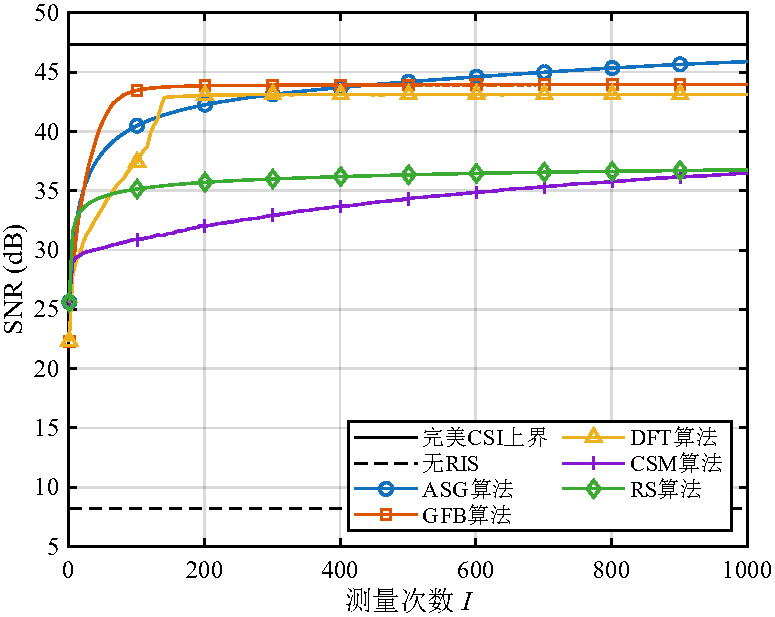
\includegraphics[width=0.6\linewidth]{ris/ris_figSNRvsMeasureNumber.pdf}
	\caption{不同算法下RIS系统可达信噪比随测量次数的变化曲线}
	\label{fig:ris_figSNRvsMeasureNumber}
\end{figure}

此外，在线传输能力是衡量算法实用性的关键。GFB 与 ASG 采用贪婪保留准则，除了一次探测的时隙可能由于相位变化导致信噪比短暂波动外，信噪比在宏观上呈现单调递增的趋势，从而支持边传输边优化的模式。
而 CSM 与 RS 算法因持续施加随机相位配置，其瞬时信噪比长期在低水平波动，在测量结束前用户几乎无法正常通信，导致系统的吞吐量较低。


\begin{figure}[!htbp]
	\centering
	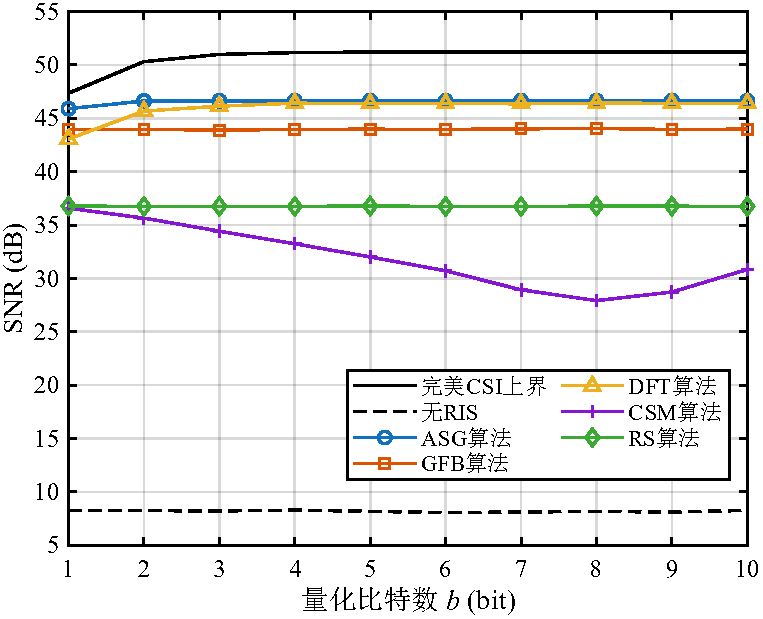
\includegraphics[width=0.6\linewidth]{ris/ris_figSNRvsPhaseBit.pdf}
	\caption{不同量化比特数下各波束赋形算法的可达信噪比表现}
	\label{fig:ris_figSNRvsPhaseBit}
\end{figure}

接下来，考虑相移量化比特数$b$对系统可达信噪比的影响。如图~\ref{fig:ris_figSNRvsPhaseBit}所示，随着$b$的增加，完美CSI上界在$b \le 3$时有明显提升，随后趋于饱和，这表明$3$比特的量化精度已基本逼近连续相移的物理极限，继续增加比特数带来的边际增益很小。
在所考虑的盲波束赋形方案中，ASG算法与DFT算法的效率随$b$的增加略有提升，但当 $b \ge 3$ 后同样趋于平缓。这是由于在有限的功率测量次数下，ASG算法难以在呈指数级膨胀的解空间中进行充分探索。
GFB算法与纯随机RS算法的性能在整个量化比特数增加的过程中保持恒定。特别是GFB算法，其行列翻转的探测机制只利用了 $1\text{-bit}$ 的自由度，适合部署于低成本的单比特RIS原型系统中。
与上述算法不同的是，CSM算法的效率随着$b$的增加出现了衰退的现象。这是由于CSM算法必须将有限的测量信息分配到反射单元的所有离散状态上，当$b$增加导致状态数骤增时，单个状态分配到的测量样本匮乏，致使条件均值估计的准确性大幅下降，最终其性能甚至劣于完全不依赖采样的RS算法。

\begin{figure}[!htbp]
	\centering
	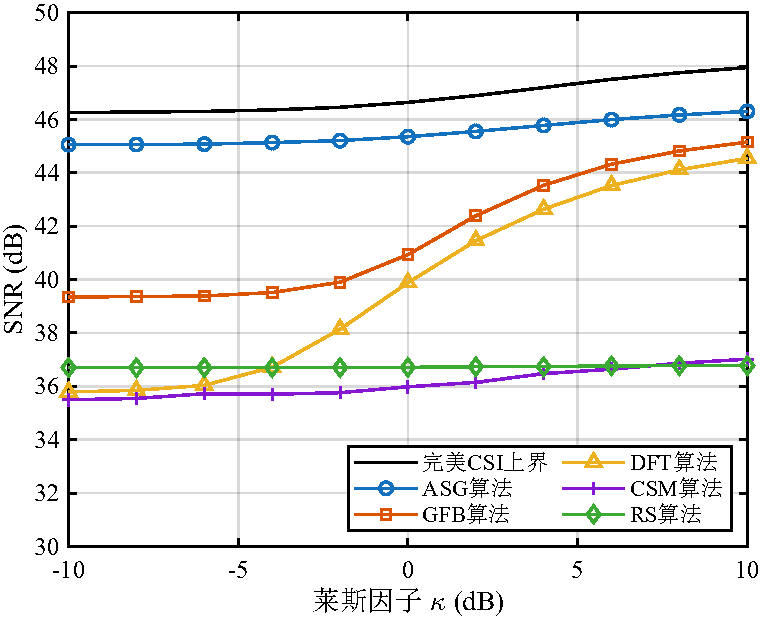
\includegraphics[width=0.6\linewidth]{ris/ris_figSNRvsRicianKfactor.pdf}
	\caption{可达信噪比随莱斯因子 $\kappa$ 的变化曲线}
	\label{fig:ris_figSNRvsRicianKfactor}
\end{figure}

进一步考察莱斯因子 $\kappa$ 对系统可达信噪比的影响，以验证各算法在不同物理传播环境下的适应能力。如图~\ref{fig:ris_figSNRvsRicianKfactor} 所示，随着 $\kappa$ 从 $-10\text{ dB}$ 增加至 $10\text{ dB}$，信道逐渐由随机多径分量主导过渡为视距分量主导。在变化过程中，ASG 算法展现出了较强的环境鲁棒性，其性能曲线在整个 $\kappa$ 区间内保持平稳且始终接近完美 CSI 上界。这是因为ASG算法没有引入关于信道分布的先验假设，能够处理多径环境下的无序信道。
相反，GFB 算法与 DFT 算法更为依赖信道的视距成分。DFT 算法受限于预定义的二维空间导向矢量，而 GFB 算法的行列整体翻转机制本质上同样隐含了最优相位分布具备二维线性梯度的空间结构假设。因此，在 $\kappa < 0\text{ dB}$ 的强多径环境中，由于缺乏主导的平面波前，这两种算法的可达信噪比较低。
此外，RS 算法由于配置完全无序，曲线呈现为一条较低的水平直线；CSM 算法受限于前文提及的样本匮乏问题，其统计均值在有限的测量次数中无法准确估计，其整体性能处于较低水平。

\begin{figure}[!htbp]
	\centering
	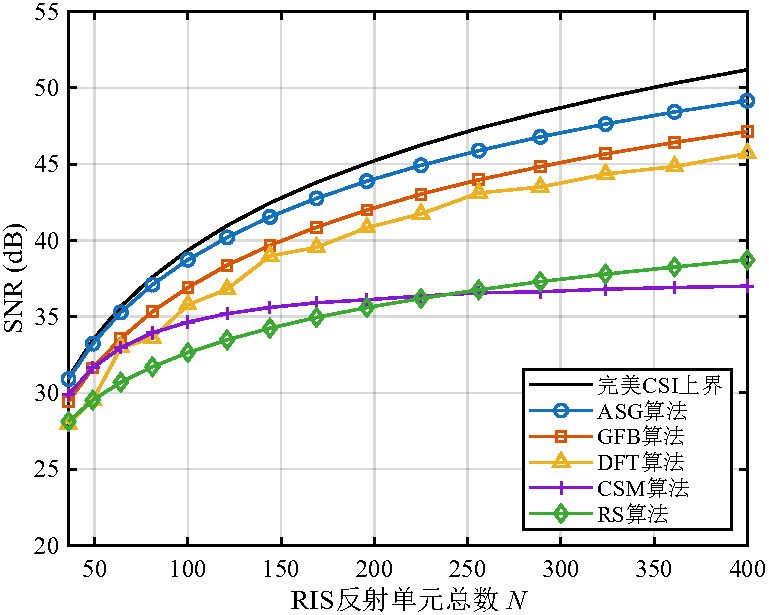
\includegraphics[width=0.6\linewidth]{ris/ris_figSNRvsRISsize.pdf}
	\caption{可达信噪比随 RIS 反射单元总数 $N$ 的变化曲线}
	\label{fig:ris_figSNRvsRISsize}
\end{figure}

最后，探讨 RIS 反射单元总数 $N$ 对系统可达信噪比的影响，以验证各算法在大规模阵列下的扩展性。如图~\ref{fig:ris_figSNRvsRISsize} 所示，随着 $N$ 从 $36$ 增加至 $400$，完美 CSI 上界呈现非线性增长，这印证了 RIS 辅助通信中接收信号功率与单元数量的平方成正比的理论特性。
在此过程中，ASG 算法的性能始终保持稳健的上升趋势，展现出较强的解空间搜索效率。GFB 算法和 DFT 算法紧随其后，在大规模部署时同样能取得可观的阵列增益。
相比之下，CSM 算法在 $N<50$ 时性能尚可，但随着 $N$ 的持续增大，其曲线迅速变缓。这说明单元数增加导致单个参数的观测样本不足，估计误差被快速放大。而 RS 算法虽无主动波束对齐，却依靠大量单元的随机叠加增益，使其信噪比随 $N$ 稳步提升，并在 $N>250$ 时反超 CSM 算法。这一对比凸显了本章所提贪婪搜索算法在大规模 RIS 盲波束赋形中的优越性与实用价值。



\section{面向 6G 的 RIS 原型通信系统设计}

本节搭建了一套软硬件协同的 RIS 原型通信系统。该系统实现了从射频收发、功率测量到状态反馈与阵列控制的完整闭环，能够运行前文提出的波束赋形算法。

\subsection{原型设计与系统架构}

作为系统的核心电磁调控节点，RIS 板卡的设计直接决定了原型的成本与性能。在文献\lcite{tan2016increasing}中，作者提出了一种可以为每个单元提供连续相移变化的RIS。其微控制器产生脉冲宽度调制信号，经过低通滤波后产生0至5 V连续变化的偏置电压。在这种方法中，每个单元的PWM信号需要独立生成，且需要相应的低通滤波电路。因此，在构建大规模RIS时，成本和硬件复杂度会大幅增加。虽然高相移分辨率在利用RIS消除多用户场景中的干扰时能够发挥重要作用\cite{wu2019intelligent}，但本章的目标是让RIS将入射波反射为指向接收机的波束。在这种场景下，低精度相位配置足以避免各单元反射的信号发生相消干涉\cite{yang2017study}。与高精度配置相比，其功率损失仅为几个分贝\cite{wu2020beamforming}。为了降低原型的复杂度，本系统采用1比特相位调控，即通过两个离散电压来表示相位差约为$180^\circ$的两种反射状态。

针对不同的测试频段与应用场景，本系统共研制了两套 RIS 面板。第一套是工作在 5.8 GHz 频段的大规模阵列，包含 1100 个反射单元，主要用于实验室及室外远距离场景的原型验证；第二套是工作在 2.6 GHz 频段的中等规模阵列，包含 256 个反射单元，主要用于与当前 5G 商用网络频段相兼容的室外覆盖增强测试。

\begin{figure}[!htbp]
	\centering
		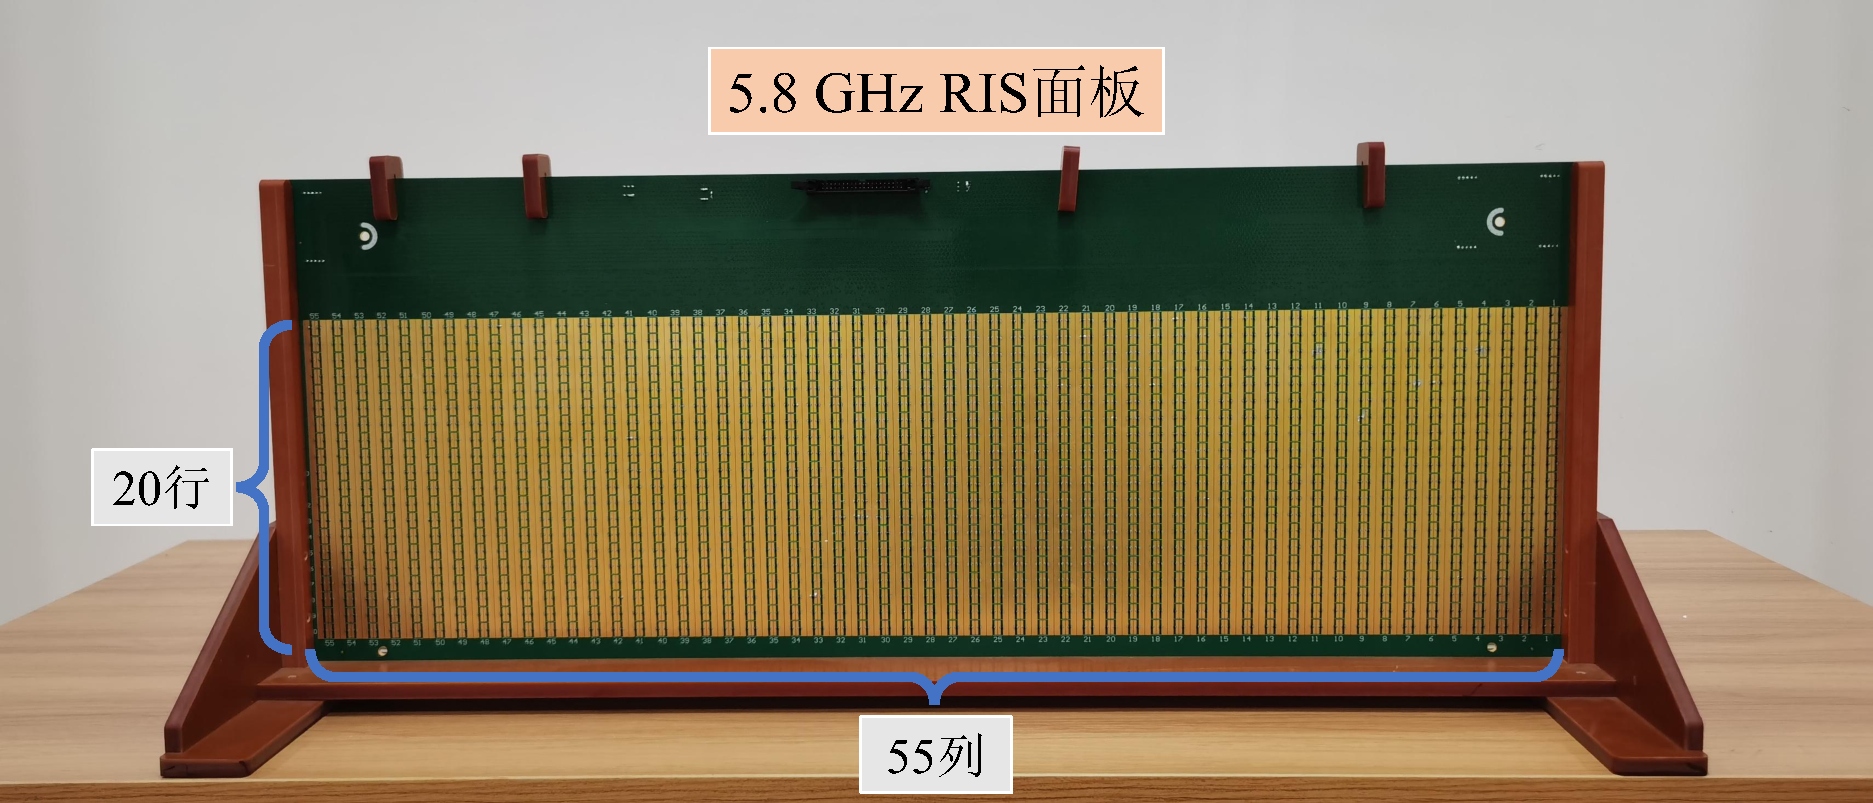
\includegraphics[width=0.6\linewidth]{ris/ris_frontview.pdf}
	\caption{工作于 5.8 GHz 频段的 1100 单元 RIS 面板实物图}
	\label{fig:ris_frontview}
\end{figure}

以5.8 GHz RIS 面板为例，其正面实物图如图~\ref{fig:ris_frontview} 所示。该RIS的尺寸为 $80.08 \, \mathrm{cm} \times 31.30 \, \mathrm{cm}$，采用均匀平面阵列布局，共包含 $55 \times 20 = 1100$ 个1比特无源反射单元，电磁反射区域的面积为$78.65 \, \mathrm{cm} \times 20.54 \, \mathrm{cm}$。在典型的无线通信场景中，用户通常在水平面内移动，而在垂直方向上的位置变化相对较小。据此，面板在布线设计上进行了分组压缩，将每一列中相邻的 5 个反射单元作为一组，共享同一路偏置电压控制信号和反射系数。因此，该RIS实际独立的控制通道数被精简至 220 路，降低了系统的布线难度与控制开销。
在阵列控制电路方面，RIS 面板的后端集成了一套基于 FPGA 的主控系统。FPGA主控板连接了 28 个 8 位串入并出移位寄存器来生成并行的离散逻辑状态，随后通过电平转换器调整输出电压幅值，使得反射单元在 5.8 GHz 工作频率下能够产生约 $180^\circ$ 的相位差。

\begin{figure}[!htbp]
	\centering
	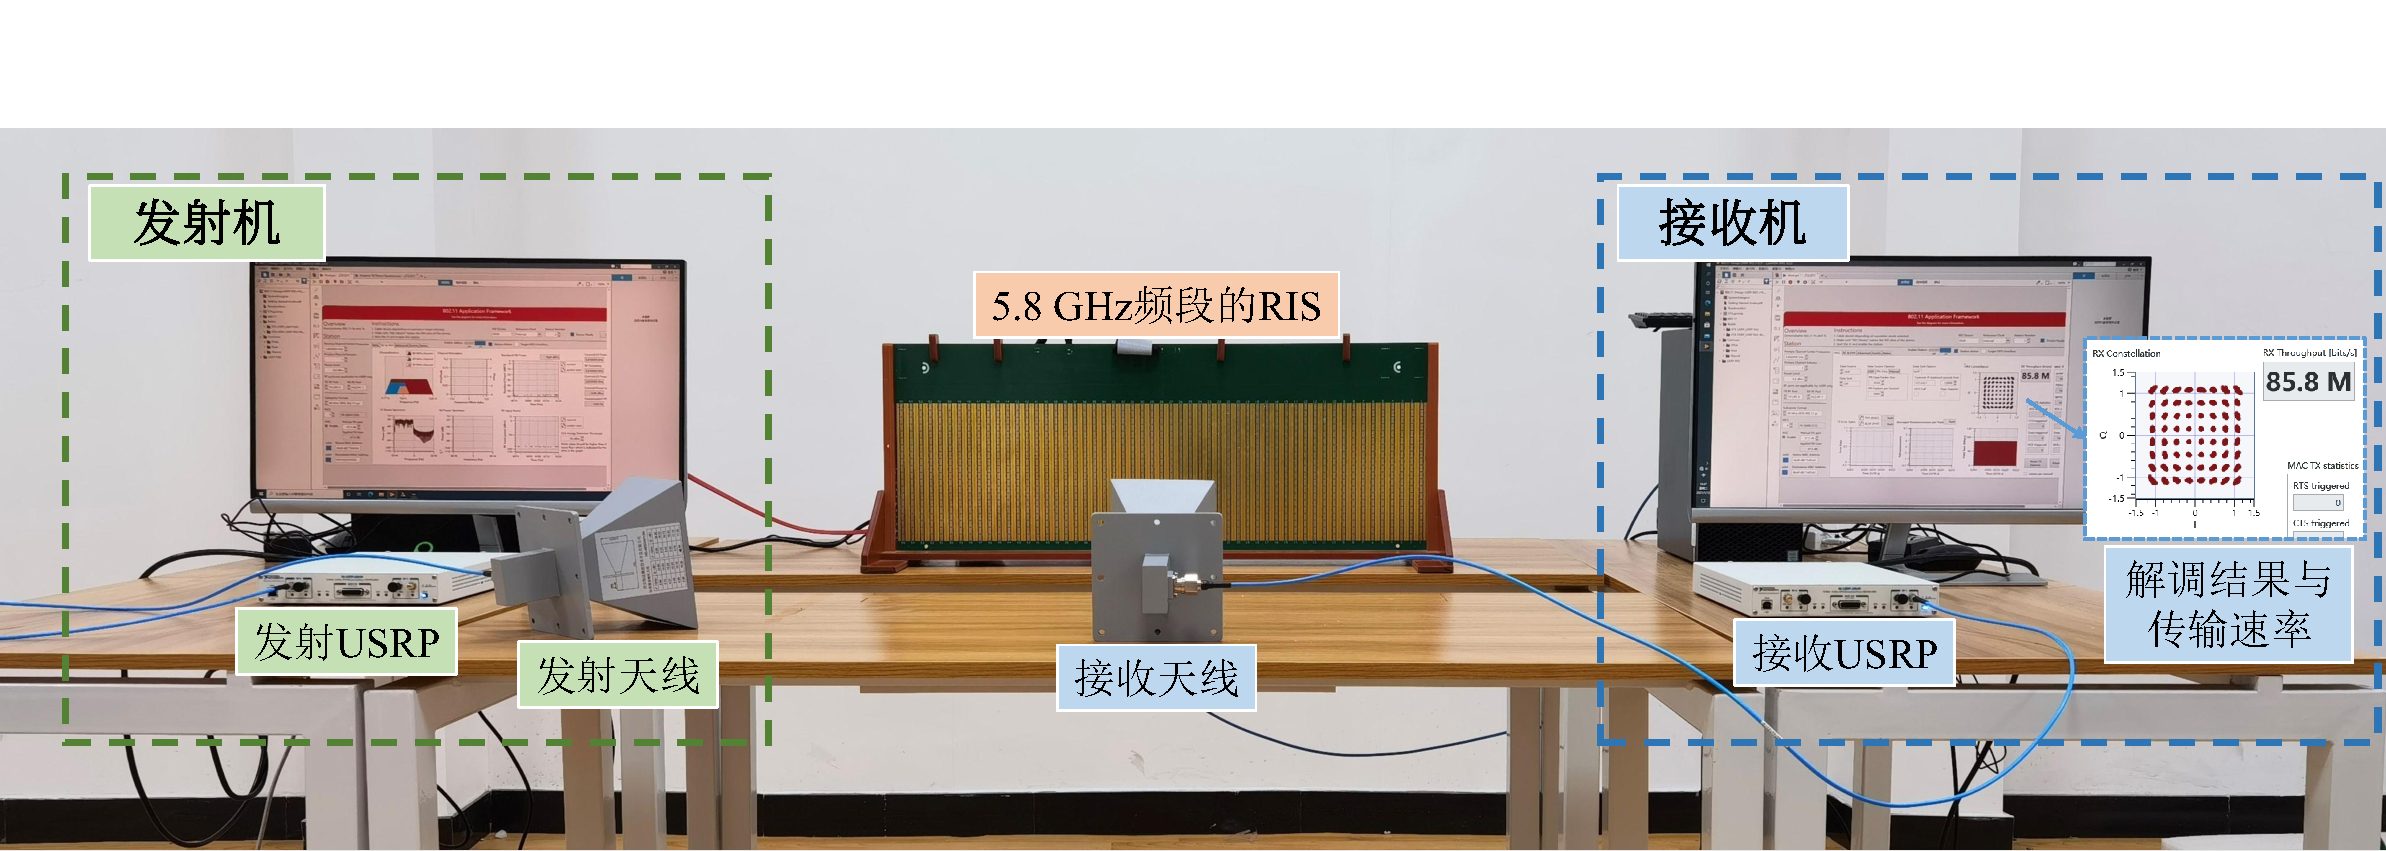
\includegraphics[width=0.9\linewidth]{ris/ris_prototype_photo.pdf}
	\caption{RIS 辅助的无线通信原型系统实物图}
	\label{fig:ris_prototype_photo}
\end{figure}

基于上述 RIS 面板搭建的完整无线通信原型系统如图~\ref{fig:ris_prototype_photo}所示。整个原型通信系统由发射机（模拟基站）、接收机（模拟用户设备）、RIS 面板及 FPGA 主控模块组成。其中，发射机和接收机均由计算机、通用软件无线电外设（USRP）及喇叭天线构成；FPGA 主控模块则包含核心板、控制电路板和实时反馈模块。图~\ref{fig:ris_system_diagram}展示了RIS辅助无线通信系统的架构框图，表~\ref{tab:ris_hardware_specs}总结了所用硬件模块的详细信息。
系统工作时，发射端通过天线发送承载高清视频流的射频信号；电磁波入射到 RIS 表面，经相位重构后反射至接收端；接收端则利用 USRP对信号进行下变频，并由上位机完成基带解调与处理。

\begin{figure}[!htbp]
	\centering
	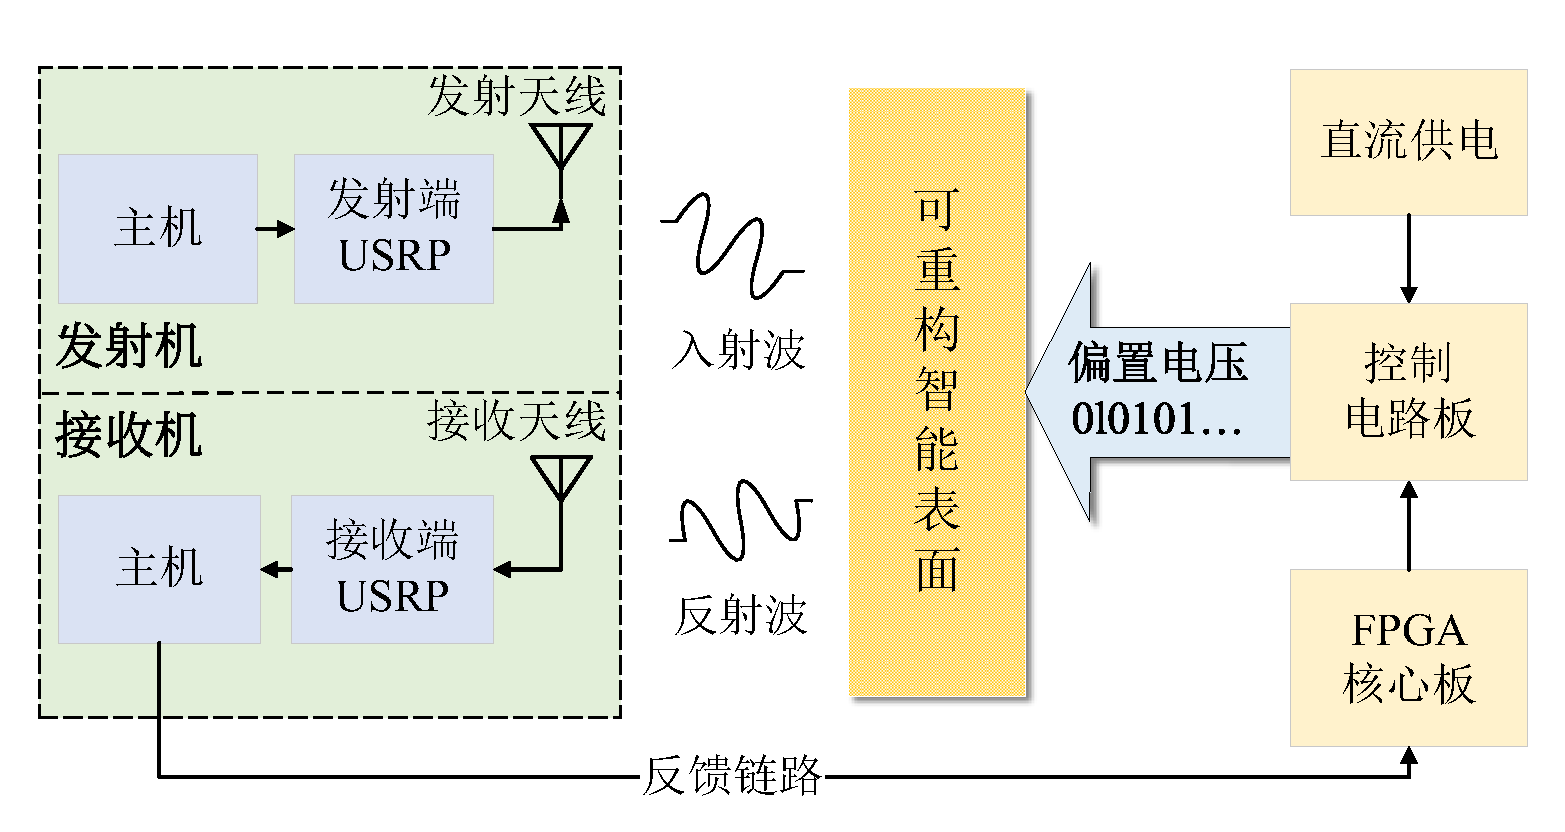
\includegraphics[width=0.6\linewidth]{ris/ris_system_diagram.pdf}
	\caption{RIS辅助的无线通信系统架构框图}
	\label{fig:ris_system_diagram}
\end{figure}

\begin{table}[!htbp]
	\centering
	\caption{原型通信系统核心硬件模块参数}
	\label{tab:ris_hardware_specs}
	\begin{tabular}{cc}
		\toprule
		\textbf{硬件模块名称} & \textbf{型号与规格描述} \\
		\midrule
		中央计算机 & 搭载 Intel Core i7-9700 处理器的通用计算机 \\
		软件无线电平台 & NI USRP-2954R \\
		主控逻辑模块 & 基于 Xilinx Zynq 7100 的开发板 \\
		喇叭天线 & 增益17.1 dBi，孔径$169 \text{ mm} \times 119 \text{ mm}$ \\
		\bottomrule
	\end{tabular}
\end{table}

为实现算法的在线迭代与波束实时追踪，系统在接收端与 RIS 控制板之间建立了一条低延迟物理反馈链路。接收机在进行基带解码的同时，实时测量当前信道的参考信号接收功率。随后，上位机通过串口将该指标实时回传至 FPGA 主控板。
FPGA 根据内置的自适应波束赋形算法进行状态评估，解算出下一时刻的最佳离散反射系数矩阵，进而驱动移位寄存器更新 RIS 单元的反射状态，完成一次波束赋形操作。
这一反馈机制无需向现有数据帧中额外插入 RIS 控制导频，使得 RIS 技术能够以透明化的方式集成至现有的无线通信网络中，避免了对终端设备的硬件升级要求。

除了具备实时波束赋形能力外，该系统还展现出了极低的功耗。RIS 的波束调控通过为变容二极管施加反向偏置电压实现，几乎不产生漏电流，二极管的总功耗仅为1.76 mW；主要的硬件功耗来自于电平转换器与稳压电路。实测数据显示，在常规波束刷新率下，这套包含 1100 个单元的 RIS 面板的总功耗仅为 0.93 W。
相较于传统基于密集射频链路的大规模 MIMO 有源天线阵列，该原型系统在能效方面展现出了数量级上的优势，从硬件层面印证了 RIS 具备低成本、低功耗部署的应用潜力。


\subsection{RIS电磁特性与波束调控验证}

本小节首先对RIS系统的信道互易性与空间波束调控能力进行验证。在当前的5G移动通信系统中，时分双工模式被广泛采用。它的一个主要特征是上行链路和下行链路的信道具有互易性。当链路的一端具有大量天线时，这是一个巨大的优势，因为可以在信道估计所需信令开销最小的方向上获取信道信息。例如，为了支持任意数量的基站天线，大规模MIMO技术正是在上行链路进行信道估计，然后将该估计值也用于下行链路的预编码。对于RIS辅助通信而言，信道互易性意味着可以将RIS配置为对下行信号进行波束赋形，随后该配置在上行方向上也能发挥同样优异的作用，而无需进行重新配置。

\begin{figure}[!htbp]
	\centering
	\begin{subfigure}[b]{0.48\linewidth}
		\centering
		 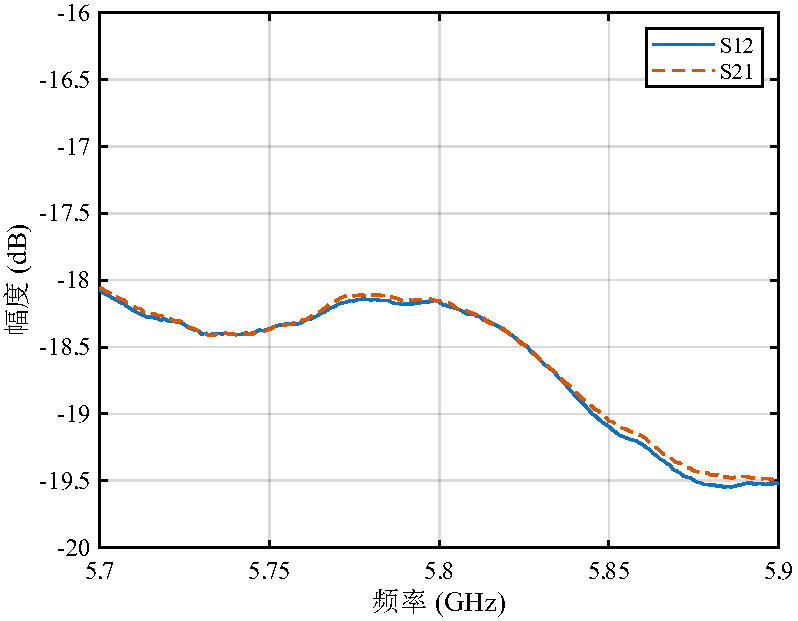
\includegraphics[height=5.8cm]{ris/ris_figChannelReciprocity_Amplitude.pdf}
		\caption{幅频响应}
	\end{subfigure}%
	\hfill % 在两个子图之间水平填充空间
	\begin{subfigure}[b]{0.48\linewidth}
		\centering
		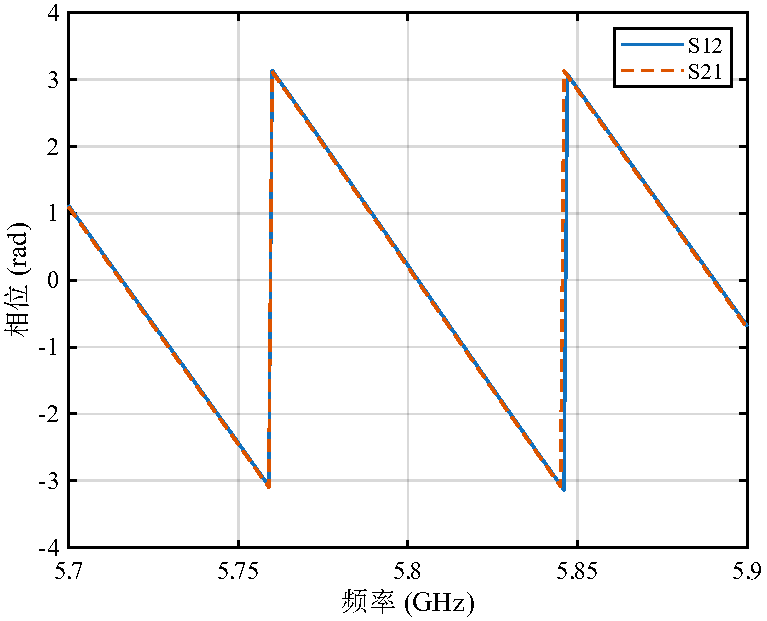
\includegraphics[height=5.8cm]{ris/ris_figChannelReciprocity_Phase.pdf}
		\caption{相频响应}
	\end{subfigure}
	\vspace{-0.5cm}
	\caption{RIS反射信道的S12与S21参数实测曲线}
	\label{fig:ris_channel_reciprocity}
\end{figure}

本小节使用矢量网络分析仪（Vector Network Analyzer, VNA）对系统的S参数进行了实测。在测试中，为尽量消除周围环境散射多径的干扰并突出RIS的纯反射信道，两副收发喇叭天线被放置在距离RIS面板0.5 m处。VNA分别向两副天线馈入测试信号，记录5.7 GHz至5.9 GHz频段内的正向传输系数S21与反向传输系数S12。
在不同天线摆放位置下进行的重复测量均显示出良好的一致性。图~\ref{fig:ris_channel_reciprocity}展示了该测试环境下的一组典型S参数测量结果。从图中可以看出，在幅频特性曲线和相频特性曲线中，S12和S21参数表现出高度的一致性。
这一结果证明了由无源超材料构成的RIS信道在宏观上服从电磁波的互易性定理。在时分双工模式下，上位机利用下行链路测得的RSRP迭代优化出的最优RIS配置向量$\bm{\phi}$，可直接应用于用户的上行信号传输。

\begin{figure}[!htbp]
	\centering
	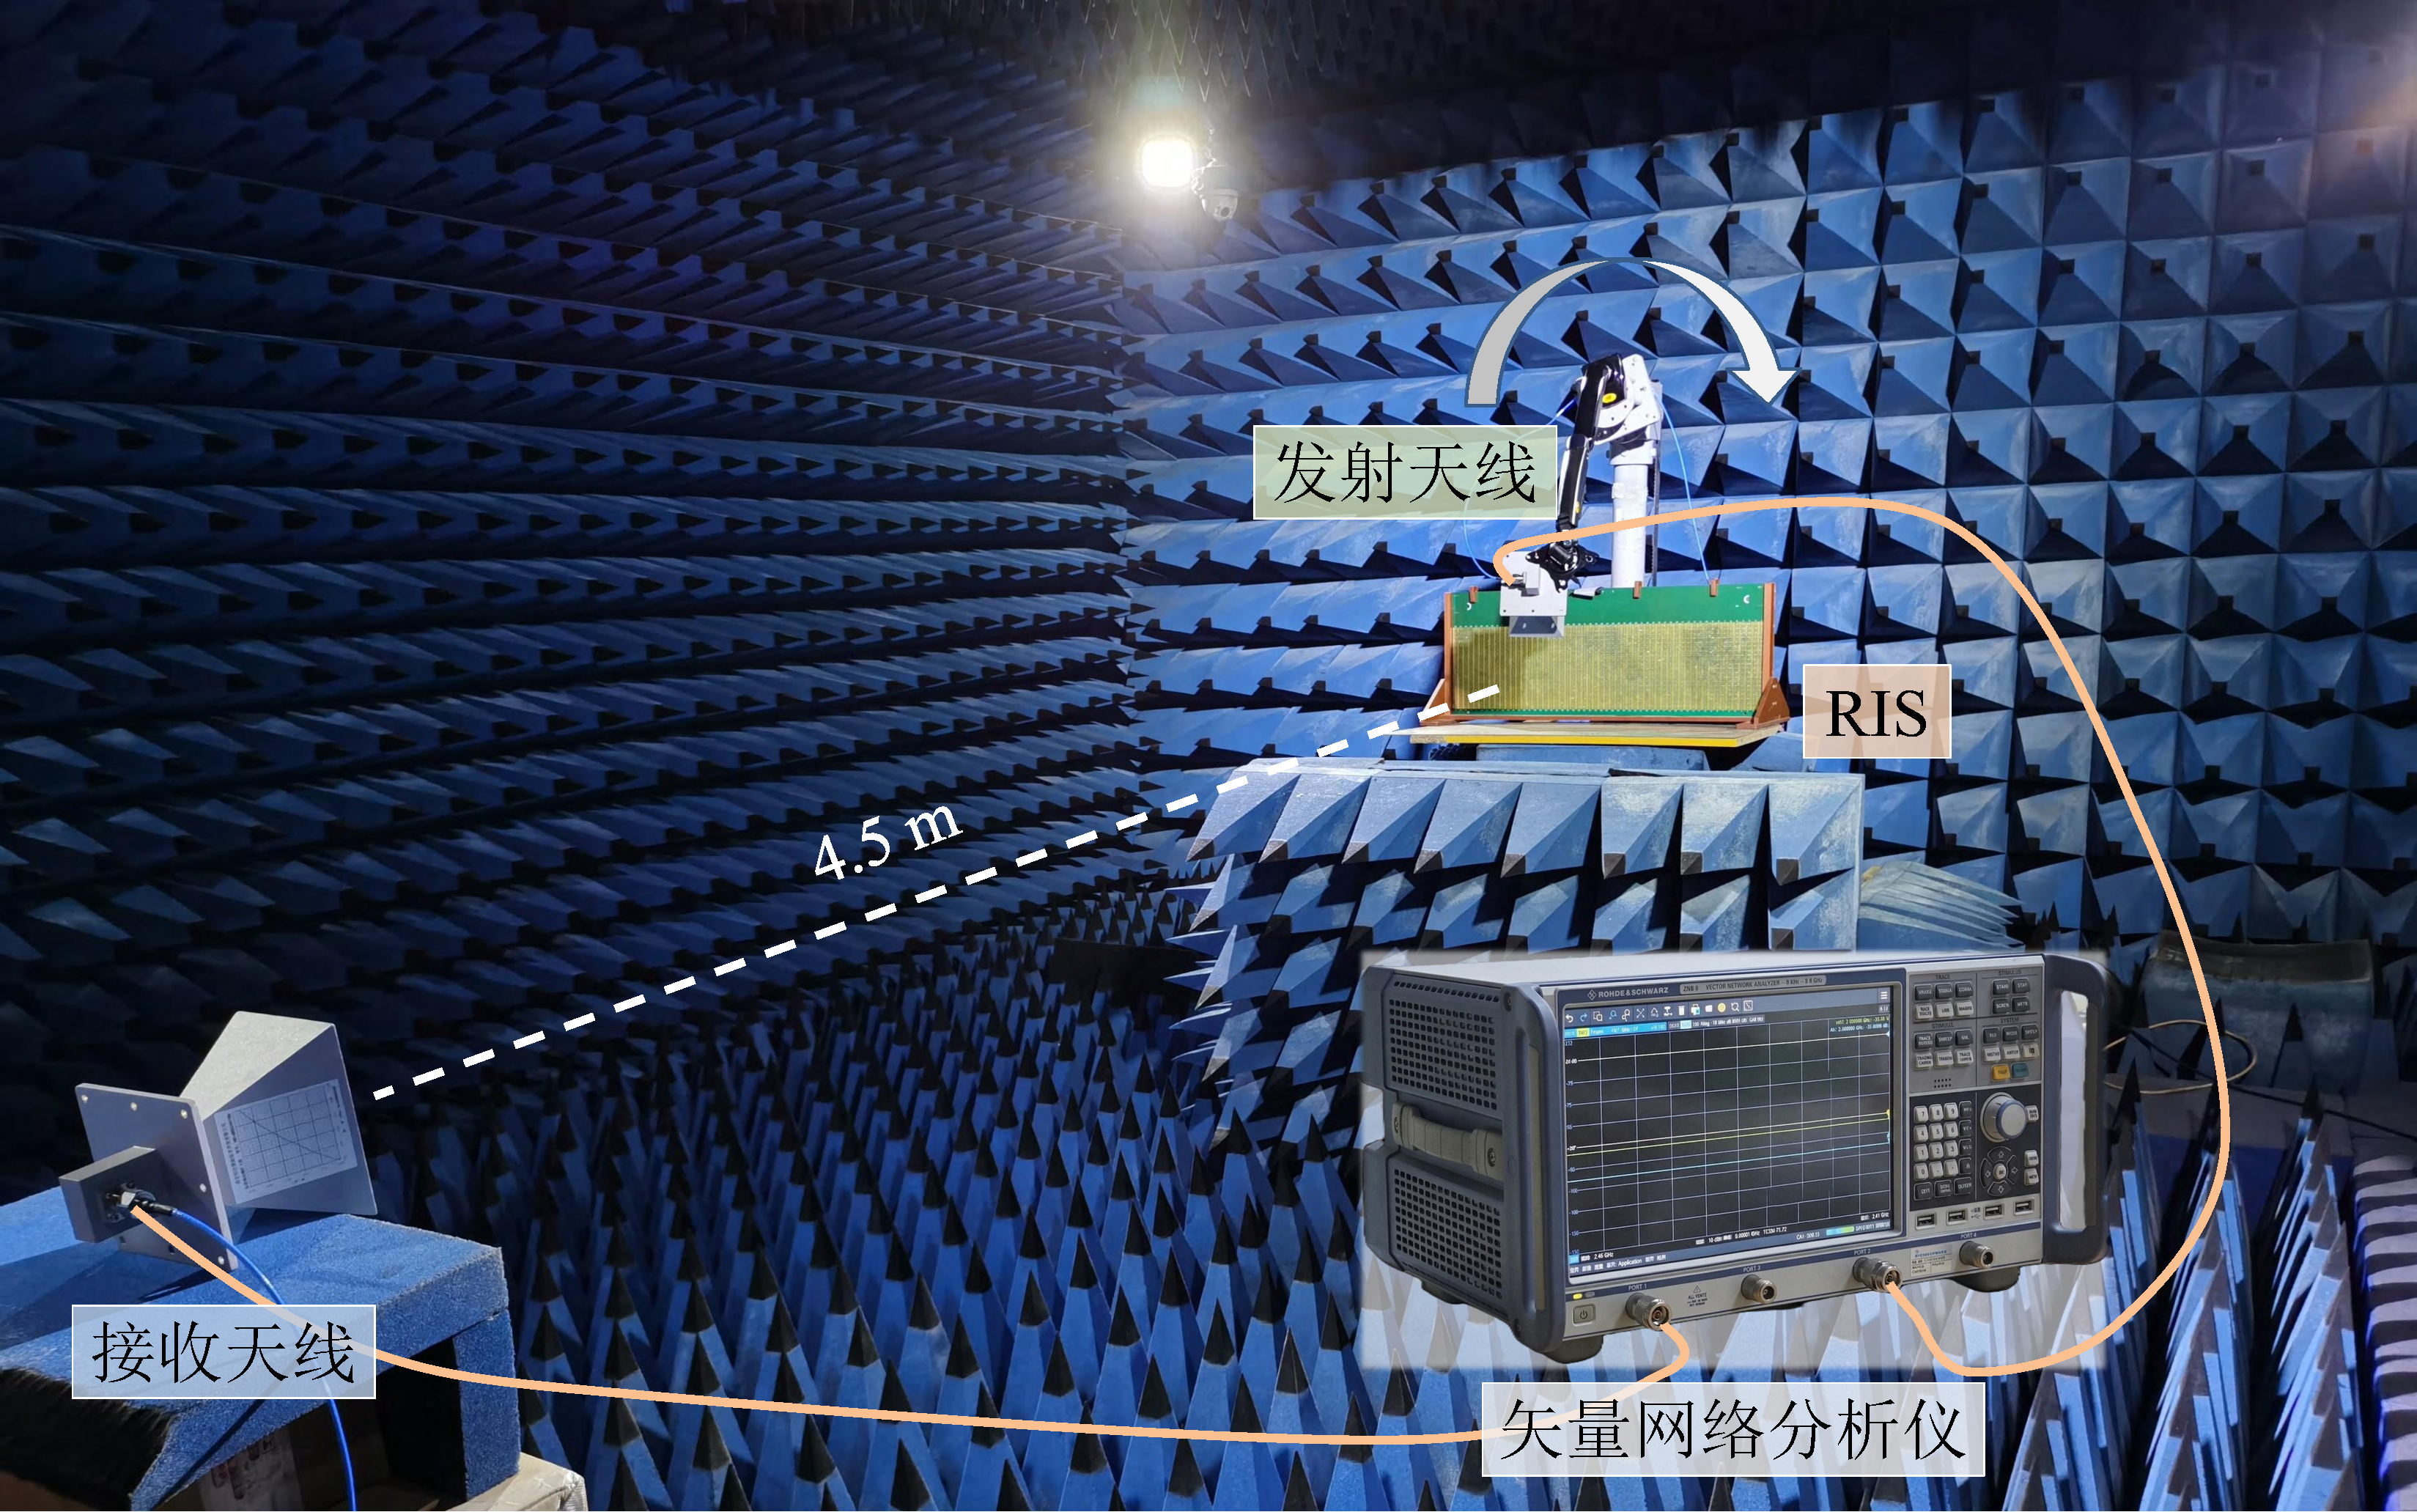
\includegraphics[width=0.6\linewidth]{ris/ris_microwave.pdf}
	\caption{微波暗室波束方向图测试环境}
	\label{fig:ris_microwave}
\end{figure}

此外，为验证RIS能否生成特定指向的空间波束，本小节在尺寸为 $7.5\,\mathrm{m} \times 5.5\,\mathrm{m} \times 3.5\,\mathrm{m}$ 的微波暗室中对RIS的辐射方向图进行了实测。如图~\ref{fig:ris_microwave}所示，测试系统由VNA与高精度转台协同构成。发射喇叭天线固定于转台延伸臂上距RIS中心 $50\,\mathrm{cm}$ 的位置，并随RIS同步旋转以维持垂直入射状态。接收天线则固定安装于距离 RIS $4.5\,\mathrm{m}$ 处的等高位置。在测量过程中，上位机通过通用接口总线协议控制转台在水平面内扫描，并同步记录 VNA 的 S 参数。

\begin{figure}[!htbp]
	\centering
	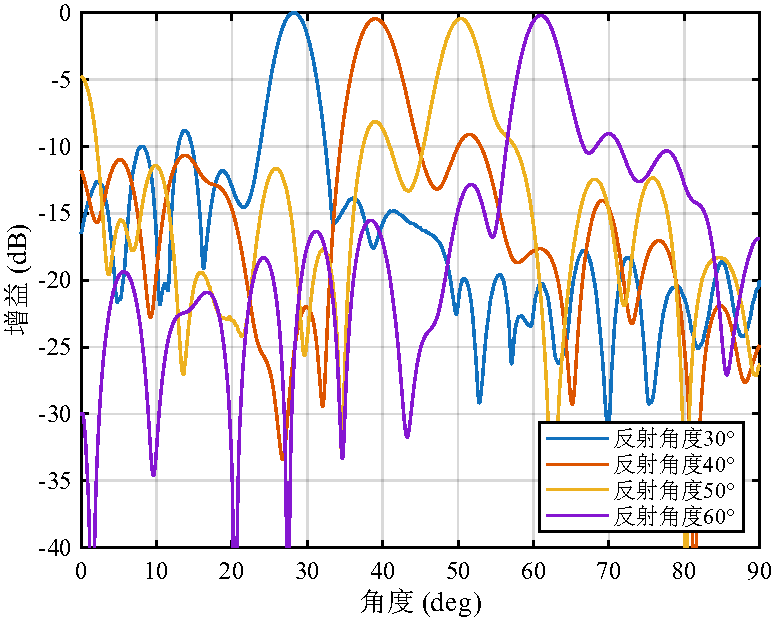
\includegraphics[width=0.6\linewidth]{ris/ris_pattern.pdf}
	\caption{垂直入射下，RIS指向不同反射角度的实测辐射方向图}
	\label{fig:ris_pattern}
\end{figure}

基于前文构建的波束赋形码本，控制器依次生成了期望反射角为 $30^\circ$、$40^\circ$、$50^\circ$ 和 $60^\circ$ 的波束赋形码字，并将其映射为 1 比特离散状态配置至 RIS。图~\ref{fig:ris_pattern} 展示了 RIS 在不同角度配置下的实测归一化辐射方向图。从图中可以看出，主瓣峰值所指向的角度与预设的期望反射角高度吻合。并且，在进行大范围的角度扫描时，主瓣的峰值增益展现出了较好的平坦度，不同指向角度下的增益波动不足 $1\,\mathrm{dB}$，且副瓣电平平均低于主瓣 $9.8\,\mathrm{dB}$。这一结果直观地验证了RIS原型系统对波束调控的准确性。


\section{RIS原型系统实测与现网应用评估}

前文已在微波暗室的理想条件下验证了所研制RIS原型系统的波束调控能力。然而，真实无线环境存在复杂遮挡与多径散射，对原型系统和算法的鲁棒性要求更高。本节将原型系统部署于实际物理环境中，依次开展室内非视距与盲区覆盖、不同波束赋形算法性能对比以及商用5G现网等多场景测试。实测中根据不同频段需求，分别采用工作于 5.8 GHz和 2.6 GHz的 RIS 面板。

\subsection{室内非视距与盲区覆盖测试}

首先，针对室内典型的高衰减与复杂多径环境，本小节分别在穿墙非视距场景和走廊、办公区边缘信号盲区场景下测试了 RIS 的覆盖补盲能力。在室内穿墙通信测试中，具体场景布局如图~\ref{fig:ris_through_wall}(a)所示，发射机部署于走廊，接收机放置于相邻的封闭房间内。收发天线之间被一堵厚度为 30 cm 的承重混凝土墙完全阻隔，墙体中间还包含一根 53 cm 厚的柱子。房间铁门处于关闭状态，不存在直接视距路径。测试过程中，发射机的发射功率设定为 $-16$ dBm。5.8 GHz RIS 被部署于房间内部，通过前文提出的GFB算法动态调整其反射系数。需要注意的是，受噪声、干扰和时变信道的影响，接收功率测量值存在一定的波动，可以通过对其进行时间平均处理，以使算法运行更加稳定。实验还引入了一块与 RIS 物理尺寸相同、且放置于同一位置的纯铜板作为对照组。

\begin{figure}[!htbp]
	\centering
	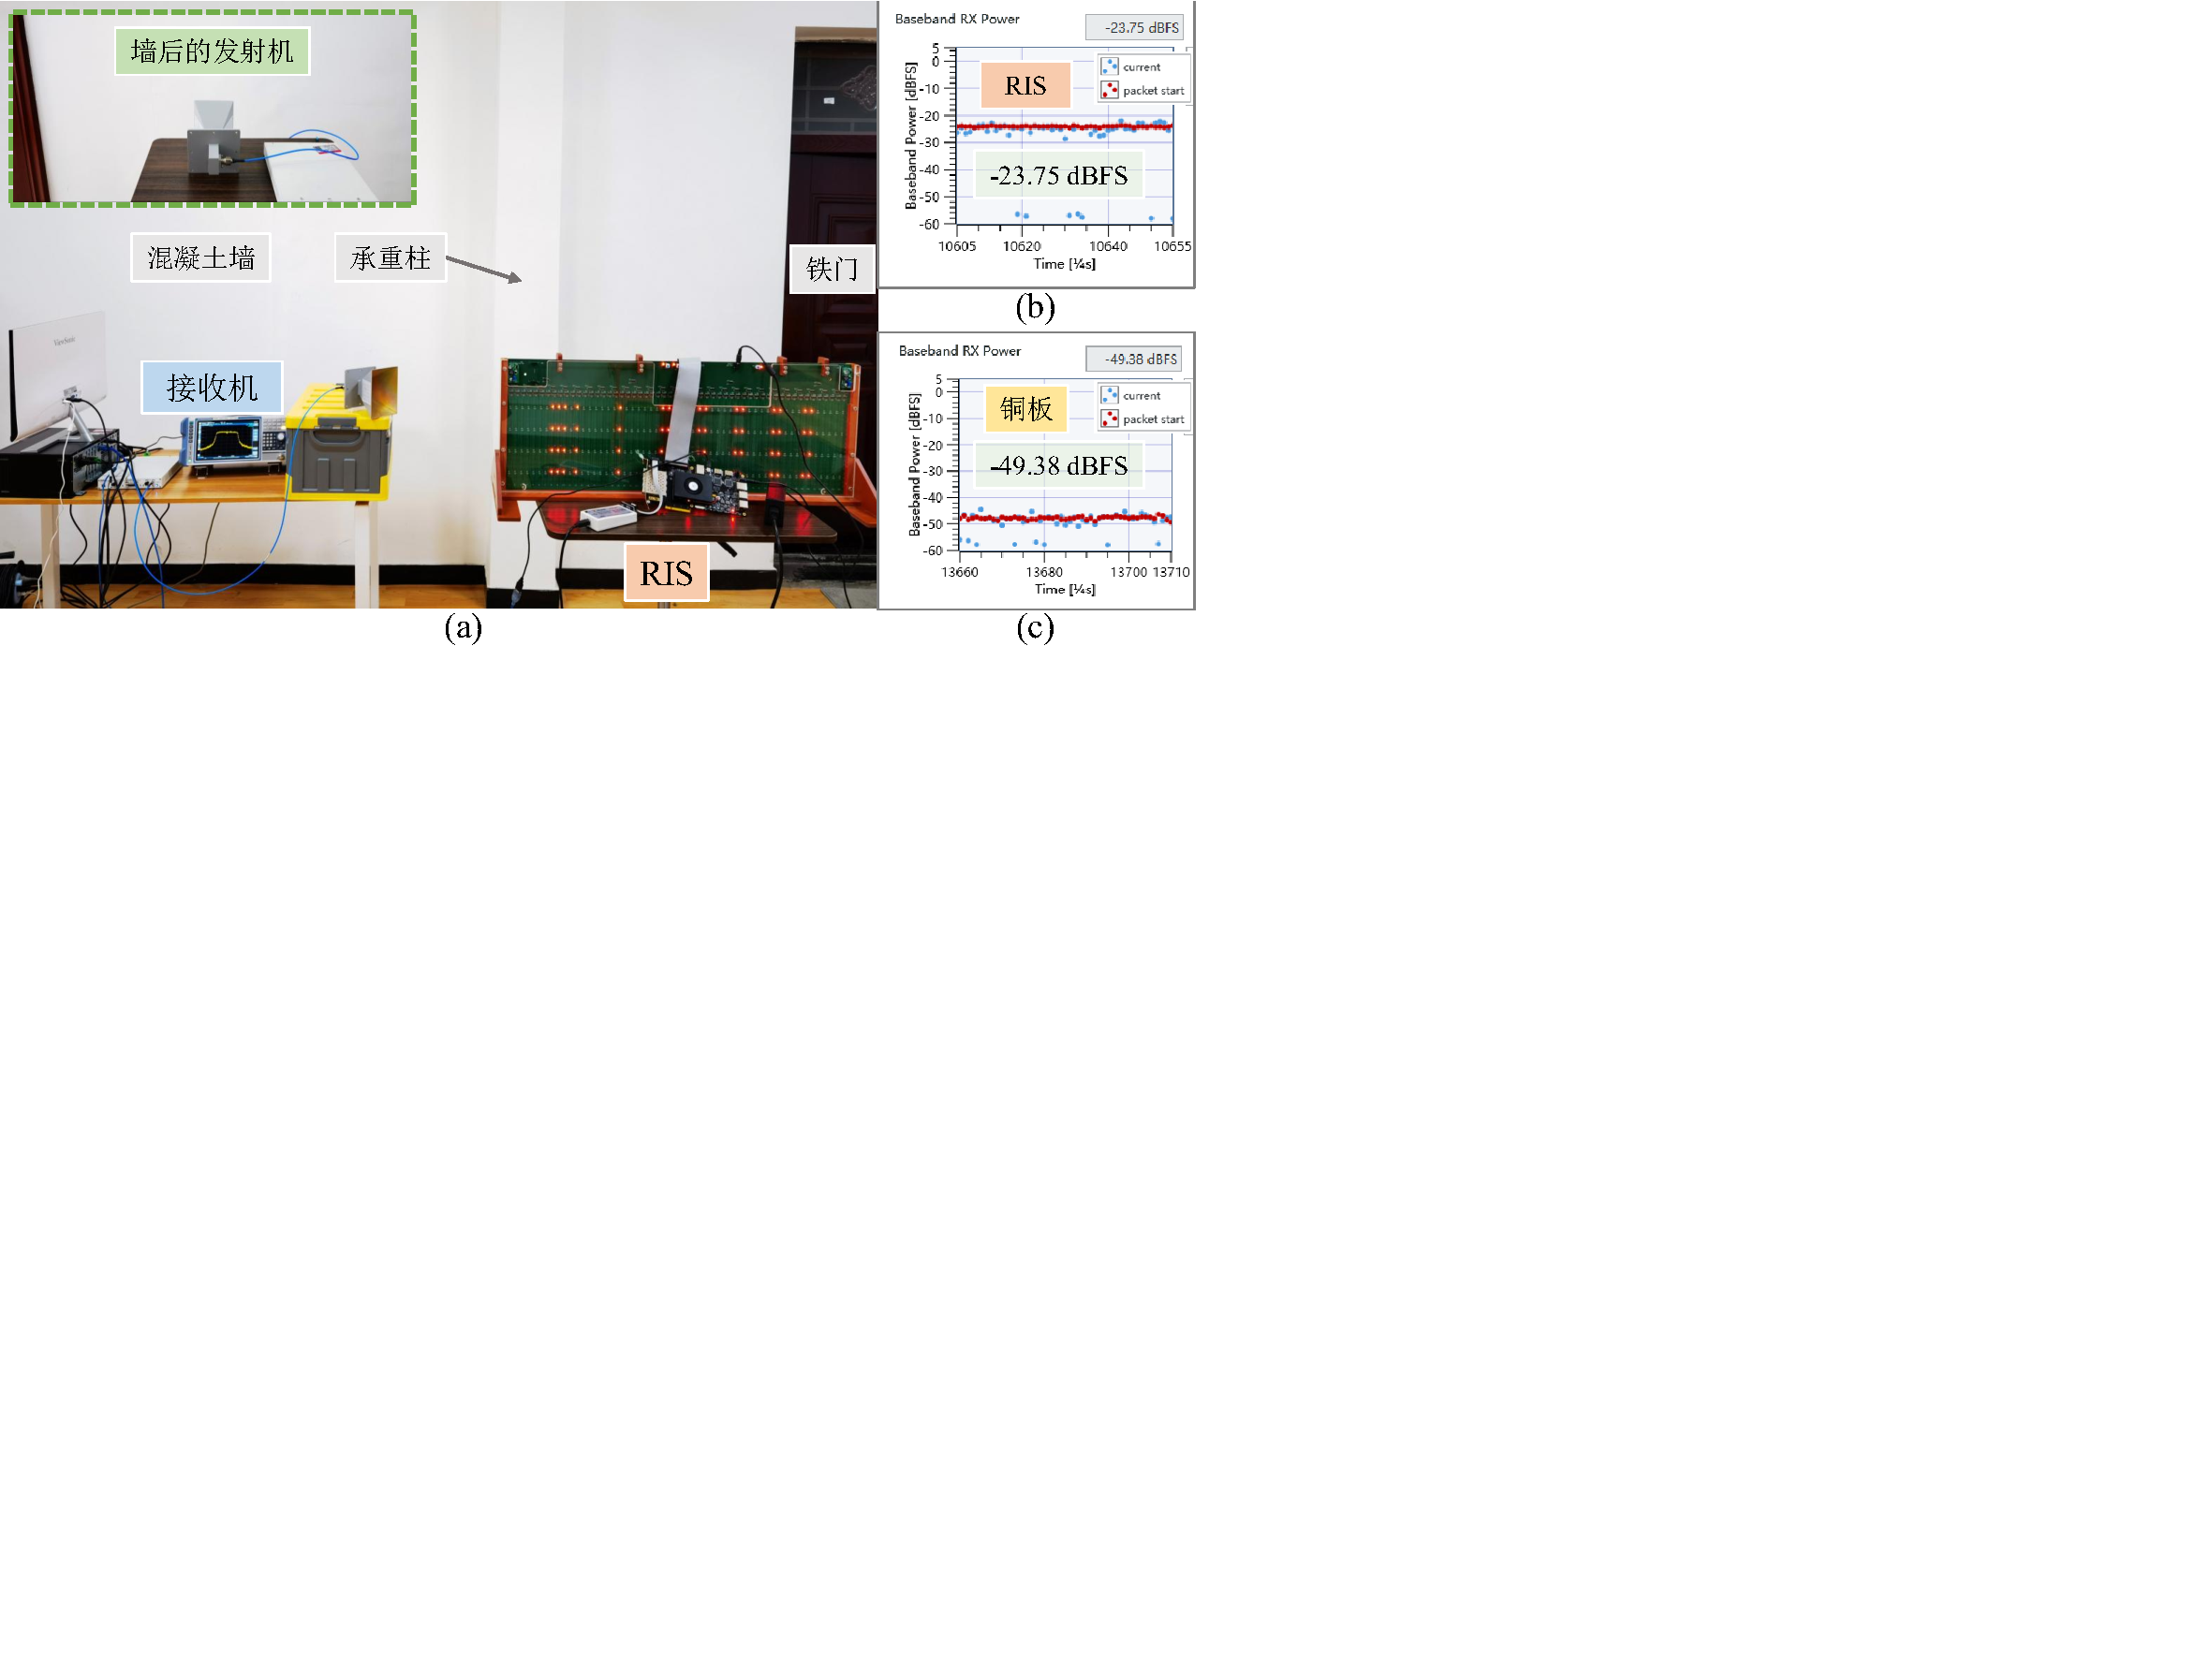
\includegraphics[width=0.7\linewidth]{ris/ris_through_wall.pdf}
	\caption{室内穿墙非视距通信测试场景及接收基带功率对比结果}
	\label{fig:ris_through_wall}
\end{figure}

图~\ref{fig:ris_through_wall}(b)和(c)展示的实测数据表明，在采用铜板反射的对照组中，接收端记录的基带信号功率仅为约 $-49.38$ dBFS，通信链路处于微弱的边缘状态；而在接入 RIS 并完成波束赋形后，基带接收功率提升至 $-23.75$ dBFS。这说明与同等尺寸的金属反射面相比，GFB算法调控的 RIS 为接收端带来了 26 dB 的功率增益。虽然普遍认为 RIS 技术在 LoS 场景下最为有效 \cite{bjornson2022reconfigurable}，但本实验证明，至少在短距离范围内，RIS 在NLoS场景下同样具有显著的增益。

\begin{figure}[!htbp]
	\centering
	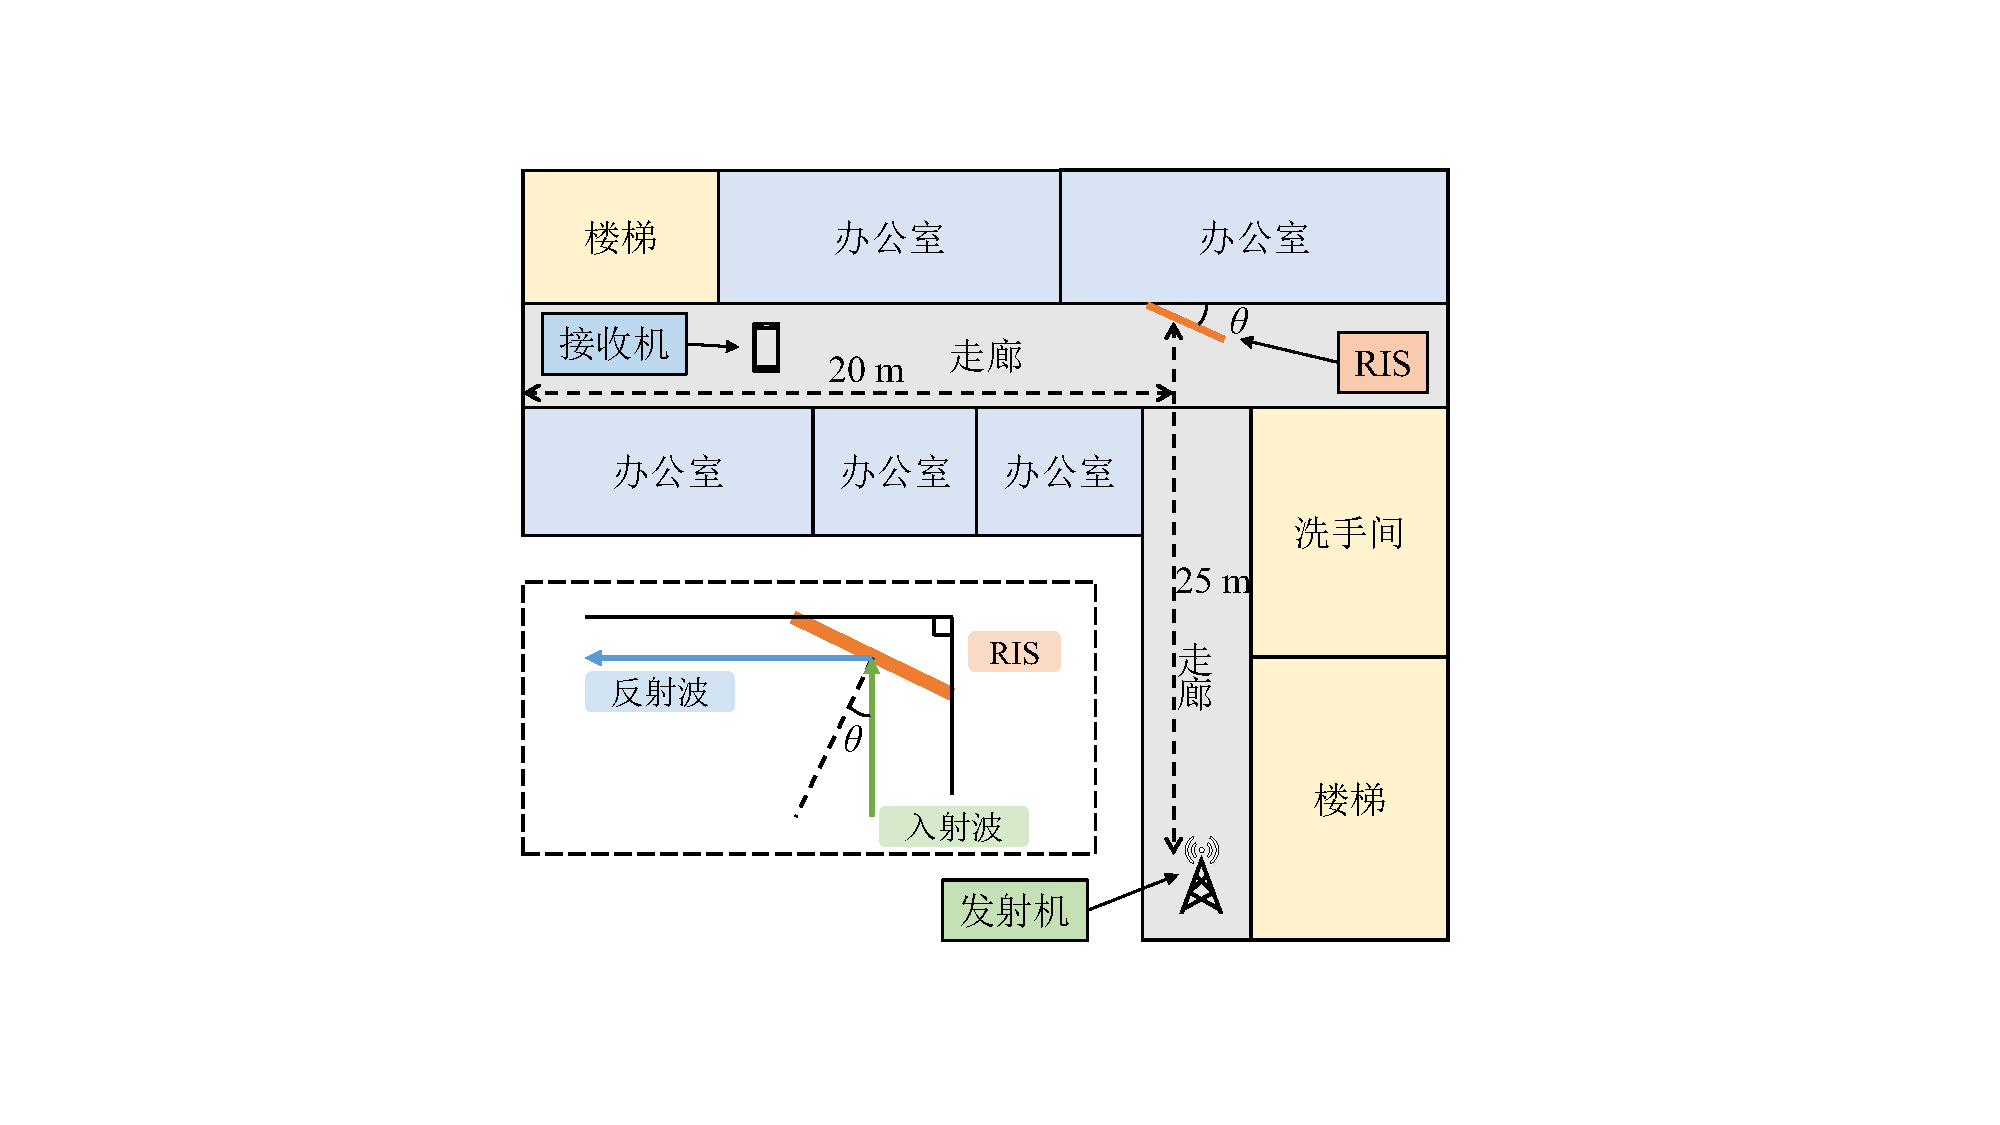
\includegraphics[width=0.4\linewidth]{ris/ris_corridor_map.pdf}
	\caption{L 型走廊盲区覆盖测试环境平面图}
	\label{fig:ris_corridor_map}
\end{figure}


现代建筑内部的 L 型走廊也是常见的电磁波传播盲区。走廊测试场景的平面图如图~\ref{fig:ris_corridor_map}所示。走廊宽度为 2.11 m，RIS 被部署于走廊拐角处，发射机和接收机分别位于两条相互垂直的走廊中。发射机到 RIS 的距离固定为 25 m，而接收机与 RIS 的距离则在 0 m 到 20 m之间，以1 m为步长变化。RIS与墙壁之间的夹角为$\theta$，该夹角同时也是入射角。发射功率为0 dBm。
首先，将接收机固定在走廊尽头，测试了不同入射角$\theta$下的接收功率。平均结果显示，与关闭 RIS 相比，开启 RIS 并完成波束赋形后，当 $\theta$ 为 $15^\circ$ 或 $75^\circ$ 时可获得 14 dB 的功率增益；当 $\theta$ 为 $30^\circ$ 或 $60^\circ$ 时增益高达 20 dB；在 $45^\circ$ 时增益约为 6 dB。

\begin{figure}[!htbp]
	\centering
	\begin{subfigure}[b]{0.48\linewidth}
		\centering
		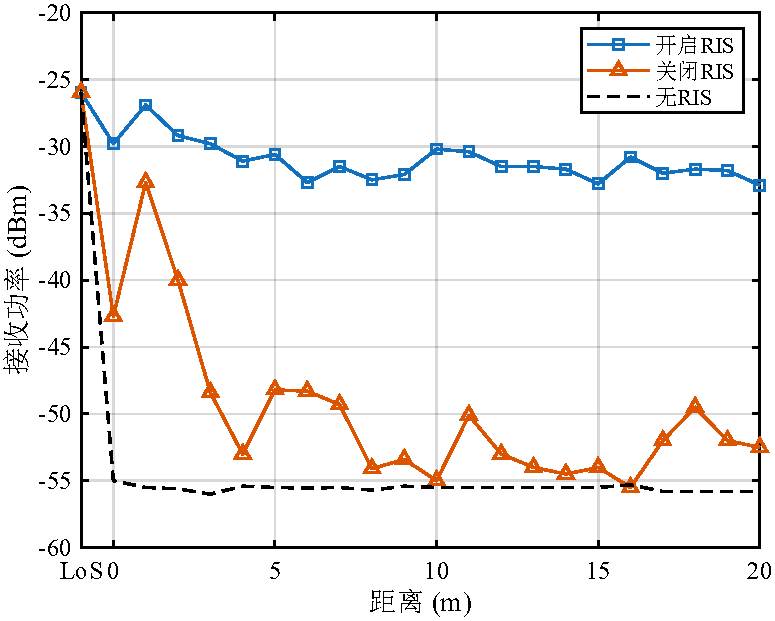
\includegraphics[height=5.8cm]{ris/ris_corridor_data.pdf}
		\caption{接收功率随距离变化曲线}
	\end{subfigure}
	\hfill
	\begin{subfigure}[b]{0.48\linewidth}
		\centering
		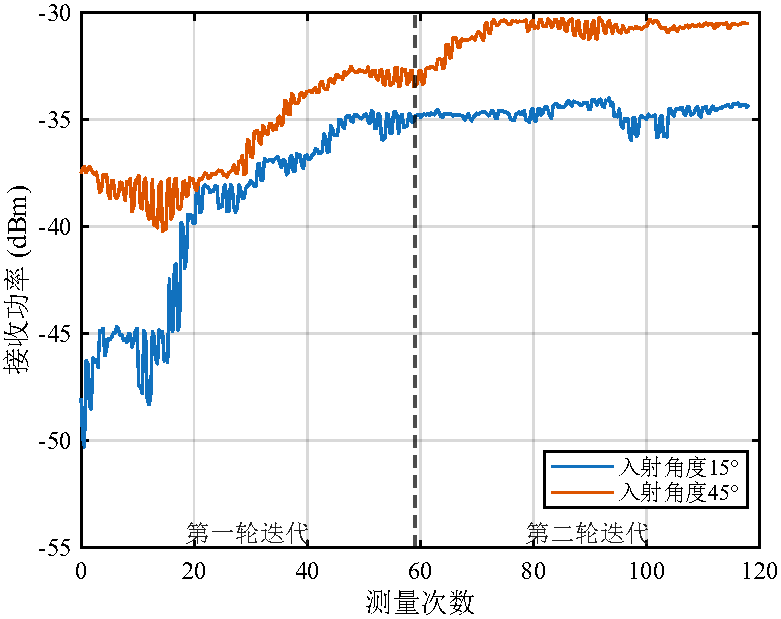
\includegraphics[height=5.8cm]{ris/ris_iteration.pdf}
		\caption{接收功率随测量次数变化曲线}
	\end{subfigure}
	\vspace{-0.5cm}
	\caption{走廊盲区覆盖性能及算法收敛性测试结果}
	\label{fig:ris_corridor_results}
\end{figure}

随后，固定入射角 $\theta = 30^\circ$，测试接收机在盲区走廊内不同距离下的接收功率，测试结果如图~\ref{fig:ris_corridor_results}(a)所示。可以看出，在没有RIS的情况下，接收功率相比视距路径下降了30 dB。随着距离的增加，处于关闭状态的 RIS仅能提供微弱且不稳定的反射，接收功率在 $-50$ dBm 以下波动。然而，当开启 RIS并运行波束赋形算法后，接收功率保持在$-32$ dBm左右。这表明，在走廊中没有直射路径的情况下，RIS可以显著增强接收功率。
此外，实验还记录了在运行GFB算法期间接收功率随时间的变化情况，如图~\ref{fig:ris_corridor_results}(b)所示。实测曲线显示，无论是在 $\theta = 15^\circ$ 还是 $\theta = 45^\circ$ 下，算法在第一轮迭代结束时，接收功率均快速爬升并趋于稳定，在第二次迭代中达到且维持了最高值。这表明GFB算法收敛较快，能够在短时间内完成盲区的波束覆盖。另外，在算法寻优过程中，接收功率未出现骤然下降的情况，具备边通信边寻优的能力。

\begin{figure}[!htbp]
	\centering
	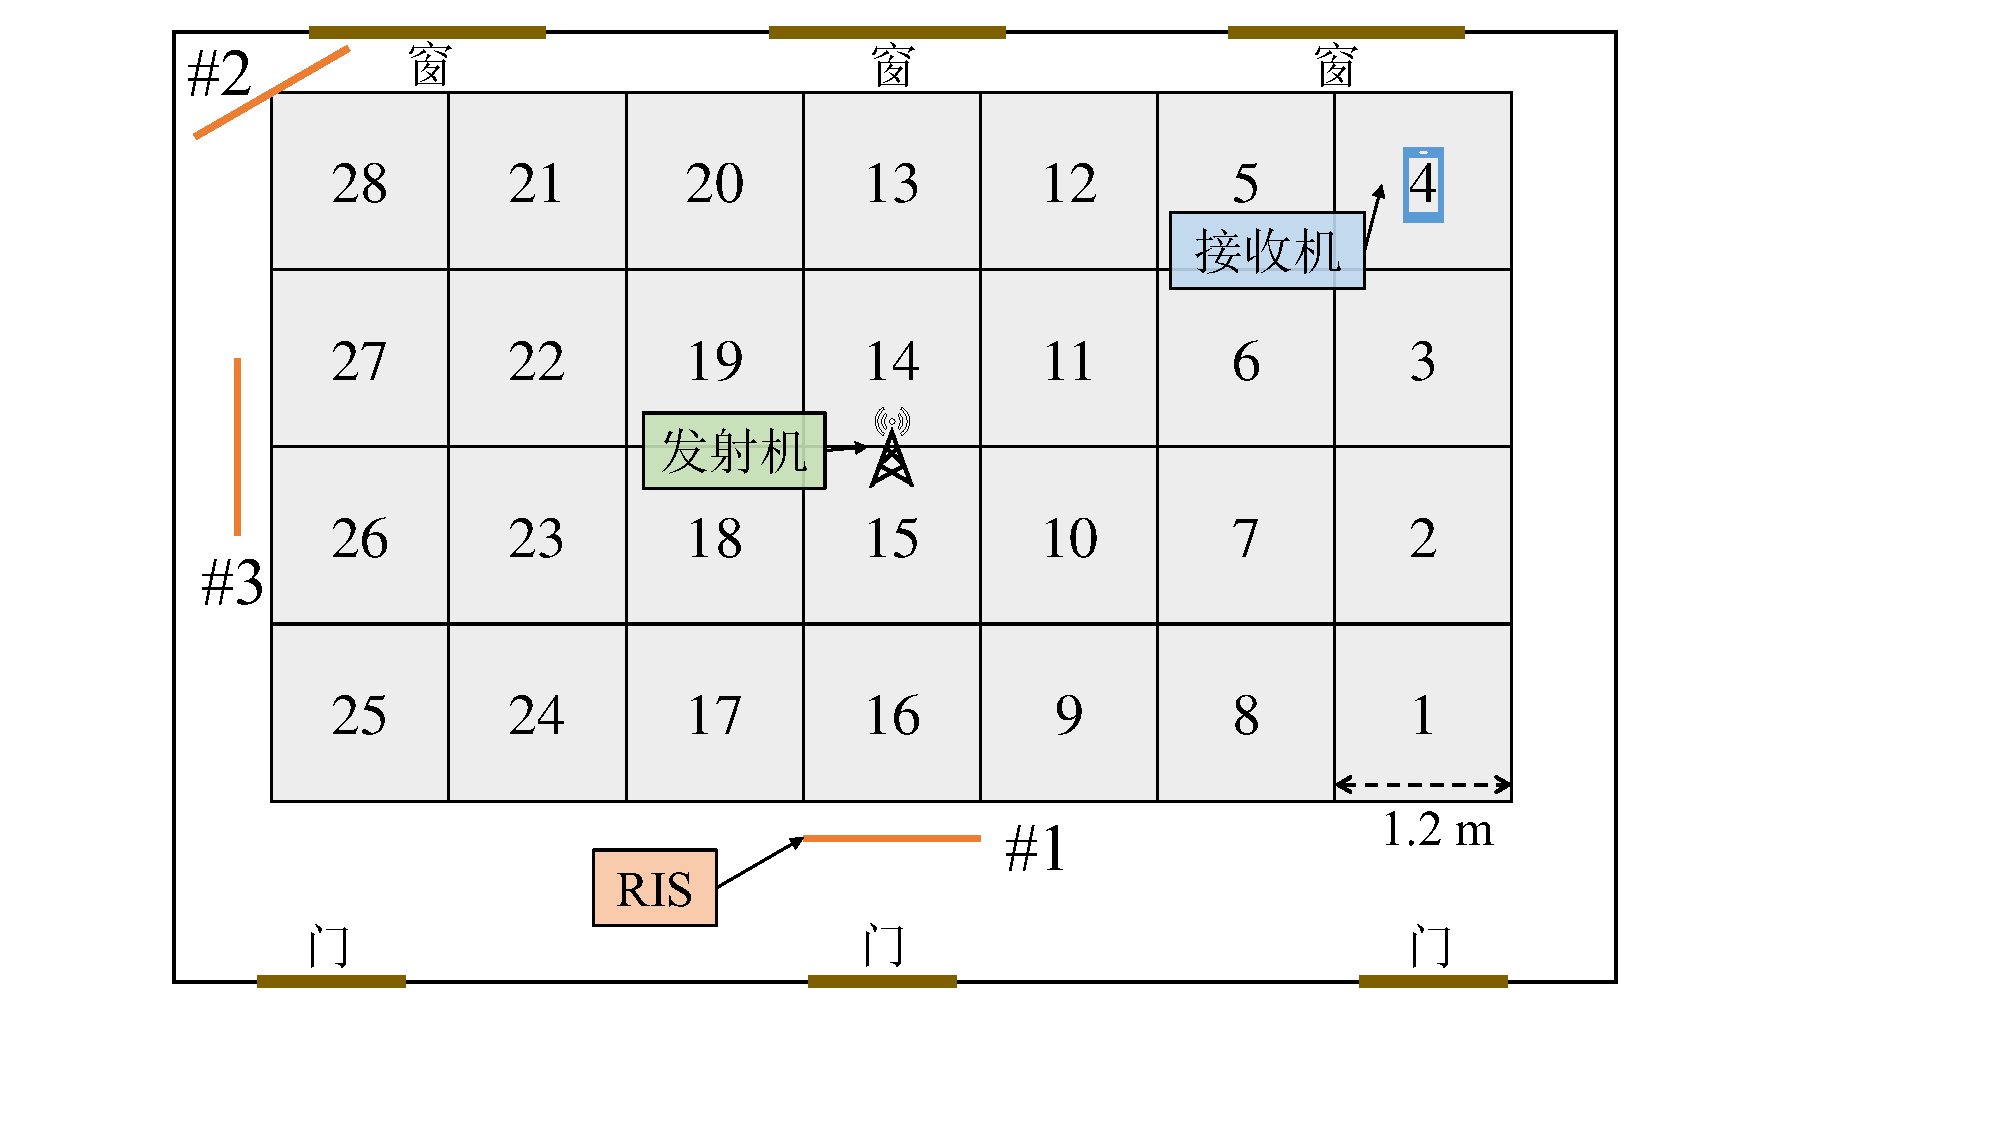
\includegraphics[width=0.5\linewidth]{ris/ris_office_map.pdf}
	\caption{室内办公区环境网格划分与 RIS 部署位置平面图}
	\label{fig:ris_office_map}
\end{figure}

为了进一步验证 RIS 在复杂室内多径环境下的补盲能力，本小节最后在一个标准的办公室内开展了边缘与角落盲区覆盖测试。如图~\ref{fig:ris_office_map}所示，该办公室被划分为 $4 \times 7$ 的网格区域，网格边长为 1.2 m。测试中，发射机固定于区域中心，发射功率设为 10 dBm，喇叭天线从发射机指向RIS的中心；接收机在 28 个网格测试点间移动，每个点停留 30 秒以记录平均接收功率。
RIS被放置在图中三个位置，定向反射波束到点4，并在整个实验过程中保持此配置不变。
实验中同样设置了同尺寸纯铜板与无反射体的基底环境作为对照组。

\begin{figure}[!htbp]
	\centering
	\begin{subfigure}[b]{0.96\linewidth}
		\centering
		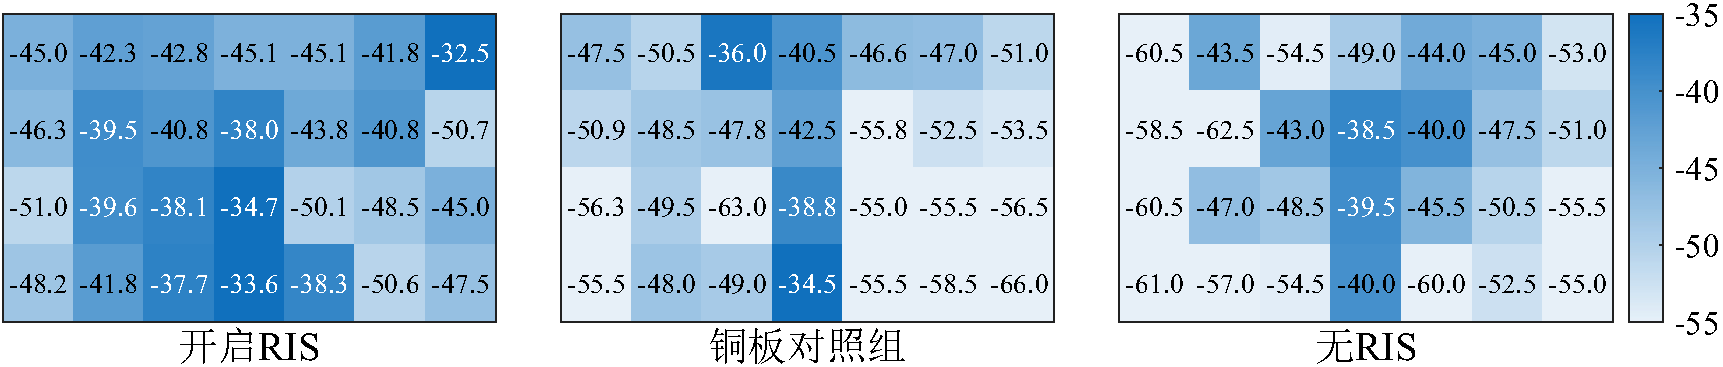
\includegraphics[width=\linewidth]{ris/ris_position1.pdf}
		\caption{RIS部署于位置1}
	\end{subfigure}
	\begin{subfigure}[b]{0.96\linewidth}
		\centering
		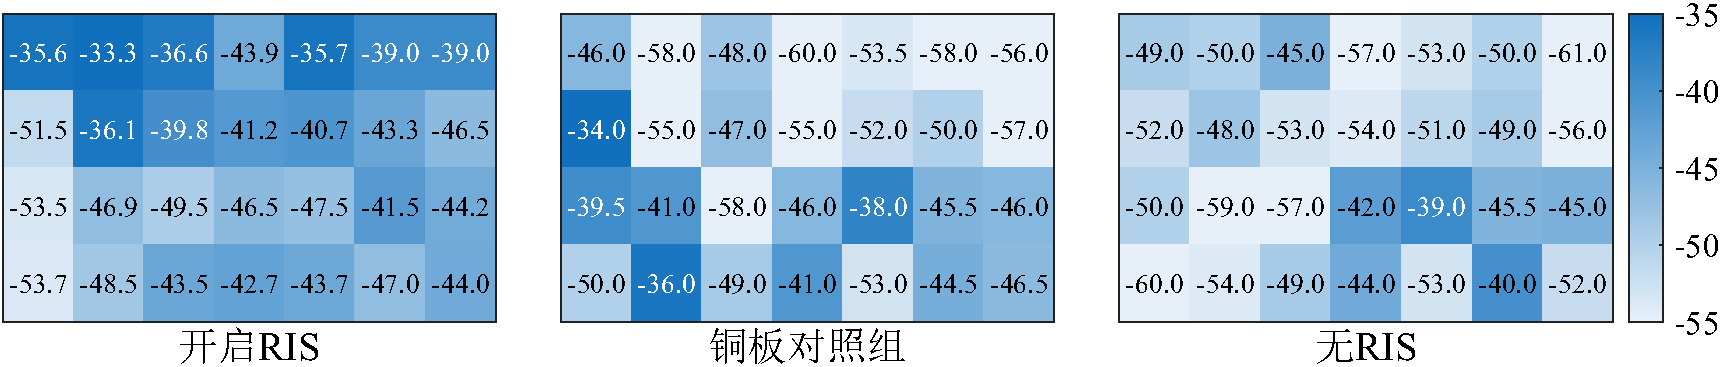
\includegraphics[width=\linewidth]{ris/ris_position2.pdf}
		\caption{RIS部署于位置2}
	\end{subfigure}
	\begin{subfigure}[b]{0.96\linewidth}
		\centering
		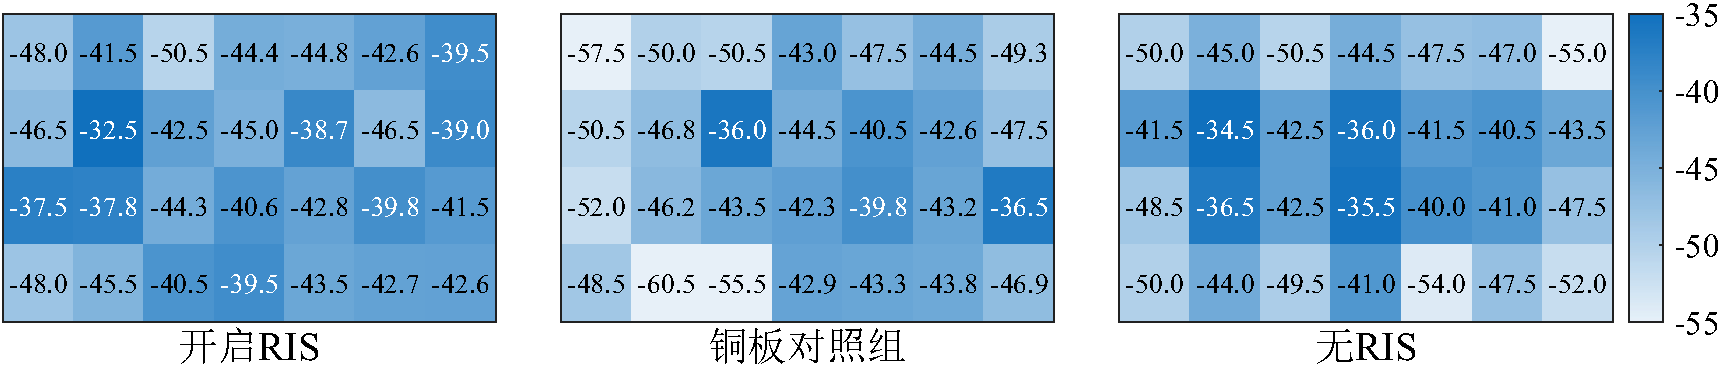
\includegraphics[width=\linewidth]{ris/ris_position3.pdf}
		\caption{RIS部署于位置3}
	\end{subfigure}
	\vspace{-0.5cm}
	\caption{不同部署位置下室内办公区各网格点接收功率空间分布图（单位：dBm）}
	\label{fig:ris_office_result}
\end{figure}

图~\ref{fig:ris_office_result}展示的测量结果表明，RIS 在复杂的室内多径环境中具有显著且普遍的信号增强效果。当 RIS 部署于墙面中部时，相比于无反射体的基底环境，运行GFB算法的 RIS 能够带来 15.5 dB 至 20.5 dB 的平均接收功率增益。其中，部署于长边中点时增益最高，相较于纯铜板提升了 18.5 dB，有效消除了整个办公区域的信号盲区；而部署于短边中点时，由于接收机与 RIS 的距离是最远的，导致接收机收到更多来自墙壁的反射信号，从RIS接收到的能量相应减少，同时，此位置的反射角是三种情况中最小的，更容易产生镜面反射，RIS的增益下降至 15.5 dB。
当 RIS 部署于办公室角落时，图~\ref{fig:ris_office_result}(b)显示，RIS 能够为目标覆盖点带来高达 22 dB 的接收功率提升，且空间连线上各点的接收功率都得到了显著增强。然而，由于在所有测试点均维持同一套码字，个别边缘测试点（如点25和点26）的接收功率仍然处于较低水平。这时，自适应调控的RIS可以快速运行算法并下发新的相位配置，将波束定向到点25处，使其接收信号功率提升至$-40.3$ dBm，较之前提高了约13 dB。
上述实验不仅证明了 RIS 在室内多径环境下能够提供稳定的覆盖增益，更反映了自适应波束赋形算法在应对动态盲区时的必要性。


\subsection{不同波束赋形算法实测性能对比}

\begin{figure}[!htbp] 
	\centering
	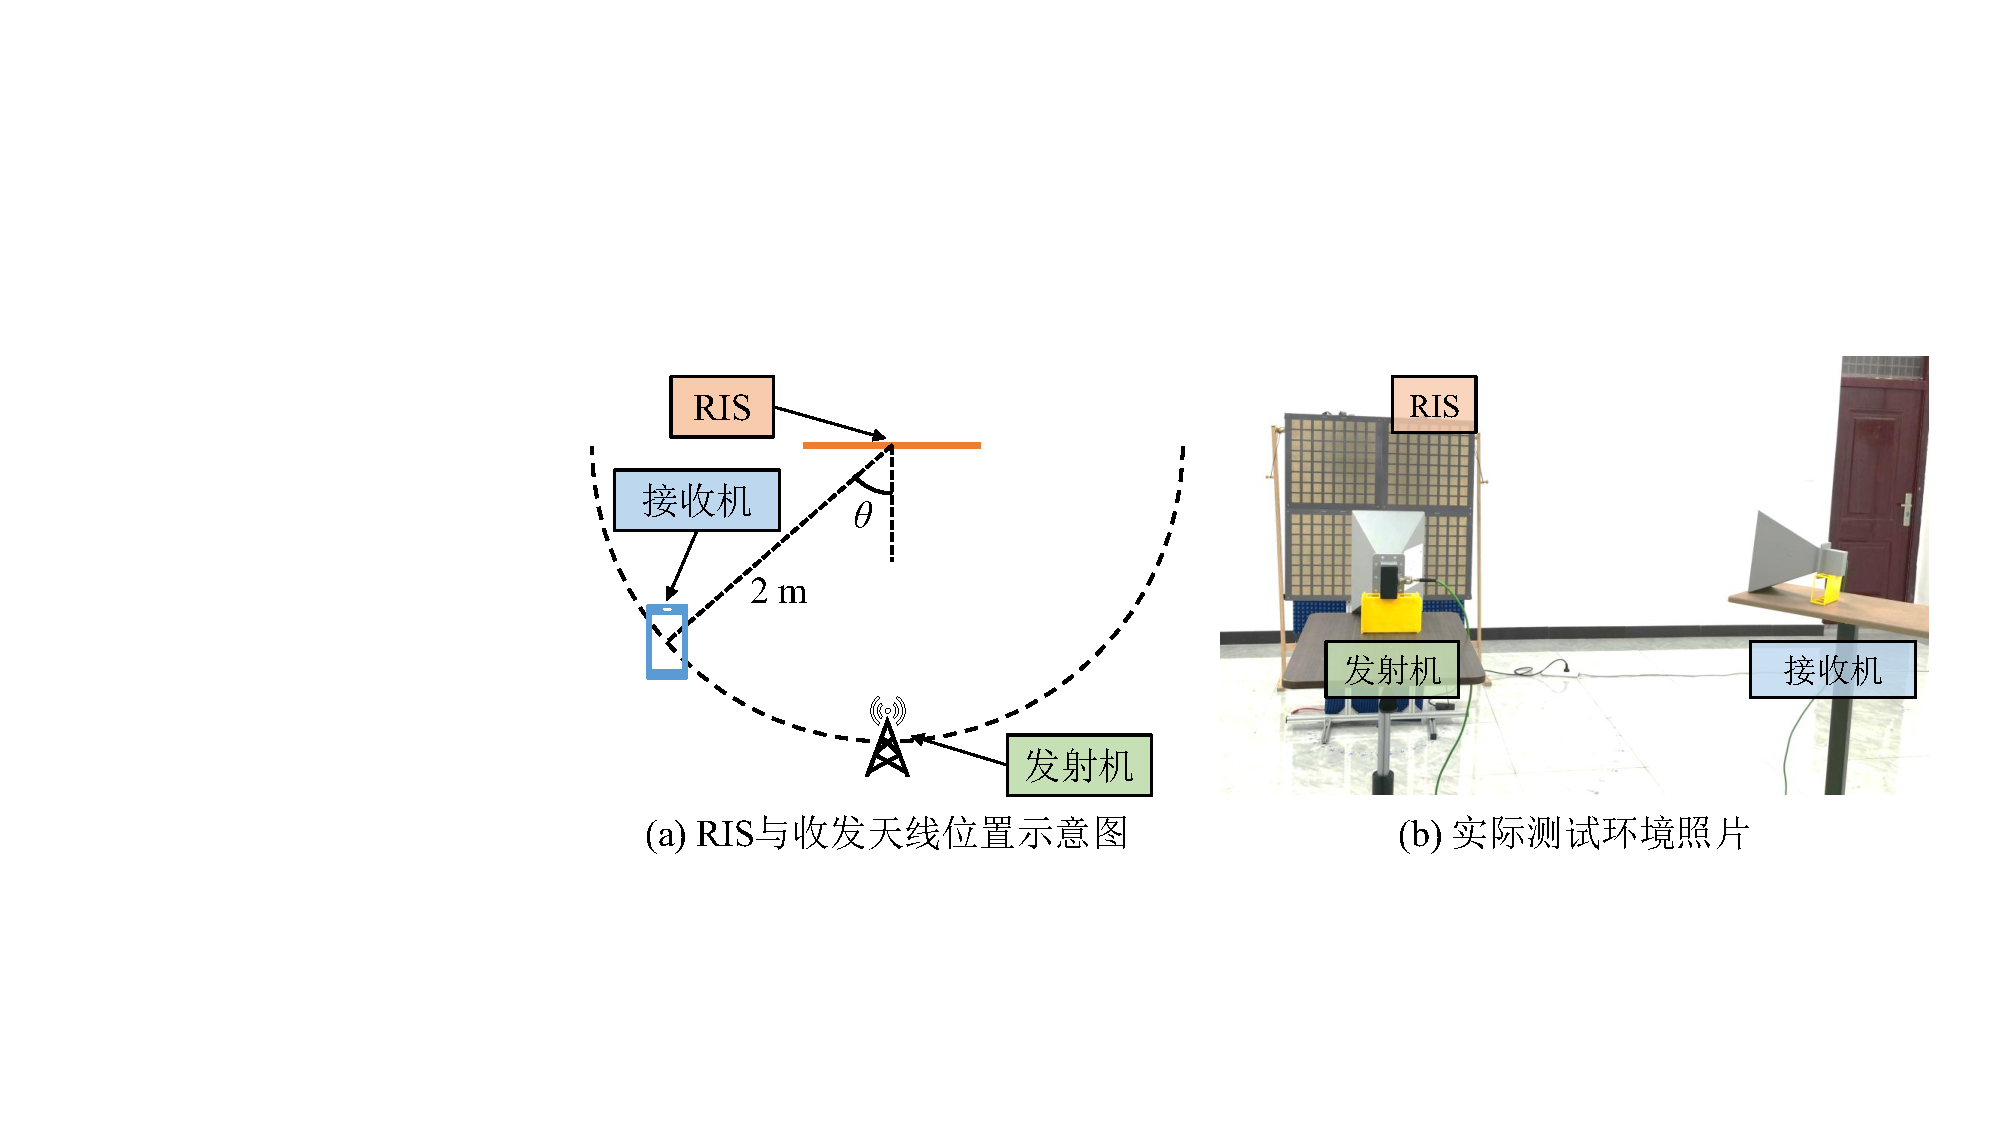
\includegraphics[width=0.8\linewidth]{ris/ris_algorithms_compare.pdf}
	\caption{实验室环境下的算法性能对比测试}
	\label{fig:ris_algorithm_test}
\end{figure}

前文的实测充分验证了 RIS 在不同场景下的盲区覆盖能力。本小节在受控的实验室环境中开展算法性能的对比测试，评估本章提出的波束赋形算法在实际物理环境中的性能。
本节测试采用了工作于 2.6 GHz 频段的 256 单元 RIS 面板。测试场景的平面布局与实物图如图~\ref{fig:ris_algorithm_test}所示。RIS 部署于房间中央，发射天线正对 RIS 面板，两者相距 2 m；接收天线沿着以RIS中心为圆心、半径为2 m的半圆移动，其与RIS法线之间的角度设置在 $30^\circ$ 至 $60^\circ$ 之间。
系统分别运行了DFT码本算法、GFB算法、ASG算法以及作为基准参考的RS算法，实验记录了在不同反射角度下，系统运行各算法完成波束赋形后相较于 RIS 关闭状态的接收功率增益。

\begin{table}[!htbp]
	\centering
	\caption{不同波束赋形算法的实测功率增益对比}
	\label{tab:ris_algorithm_comparison}
	\begin{tabular}{cccccc}
		\toprule
		\multirow{2}{*}{\textbf{算法类型}} & \multicolumn{5}{c}{\textbf{接收功率增益 (dB)}} \\ \cmidrule(lr){2-6}
		& $\theta=30^\circ$ & $\theta=40^\circ$ & $\theta=50^\circ$ & $\theta=60^\circ$ & \textbf{平均增益} \\
		\midrule
		DFT算法 & 9.5  & 10.1 & 11.4 & 11.1 & 10.5 \\
		GFB算法 & 10.0 & 10.3 & 10.3 & 10.2 & 10.2 \\
		ASG算法 & 11.1 & 12.3 & 12.8 & 11.5 & 11.9 \\
		RS算法  & 4.2  & 5.2  & 5.1  & 4.6  & 4.8  \\
		\bottomrule
	\end{tabular}
\end{table}

各算法的实测性能对比数据详见表~\ref{tab:ris_algorithm_comparison}。从表中可以看出，ASG算法展现出了最优异的性能，在所有测试角度下均取得了最高增益，平均增益为 11.9 dB，相较于 DFT 算法与 GFB 算法获得了超过 1 dB 的提升。RS算法的平均增益仅为 4.8 dB，在所有方案中表现最差。这一实测结果与第~\ref{sec:ris_simulation}节的数值仿真一致。


\subsection{商用 5G 现网环境性能评估}

为了评估RIS系统在商用网络下的性能，本小节在一处大型工业园区进行了5G现网实测。测试场景的卫星地图与现场部署情况如图~\ref{fig:ris_outdoor_map}所示。测试选定了一处室内通道信号盲区，商用 5G 基站位于室外，距走廊入口约 100 m。测试时，将 2.6 GHz 频段的 RIS 面板放置在通道入口处，其正面朝向基站方向；接收终端位于室内，距离 RIS 约 1.5 m，终端所在方向与 RIS 法线之间的夹角约为 $45^\circ$。实验中使用信号测试软件来监测来自基站的信号接收情况并记录其强度。
在不部署RIS的情况下，当用户设备在室内时，基站小区不在软件显示的小区列表中。部署RIS后，用户能够解码基站的物理小区标识，但此时的RSRP仍低于 $-90$ dBm。随后，系统运行GFB算法在线优化 RIS 反射波束。波束对准后，室内终端的 RSRP 比 RIS 关闭时提高了4至5 dB。

\begin{figure}[!htbp] 
	\centering
	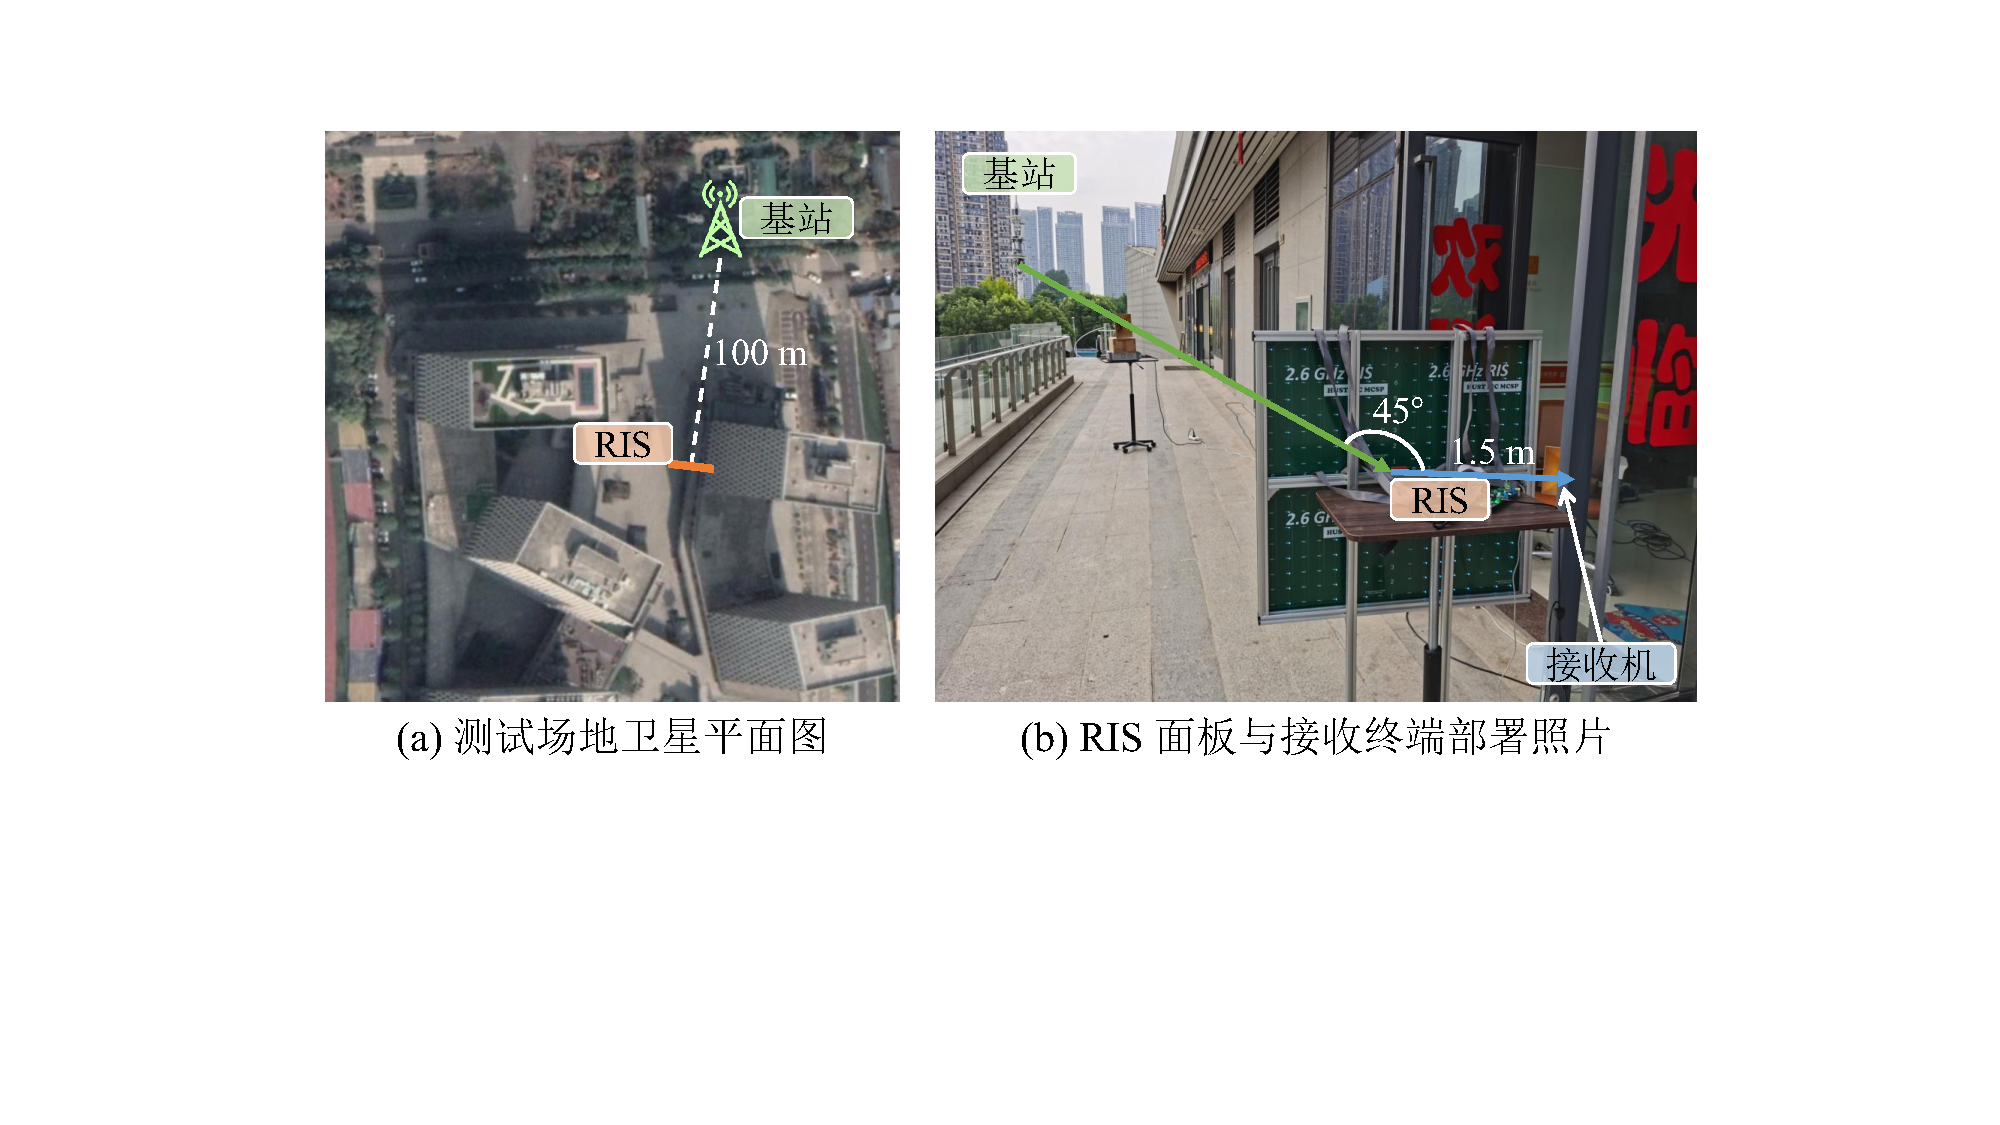
\includegraphics[width=0.7\linewidth]{ris/ris_outdoor_map.pdf}
	\caption{商用 5G 现网覆盖增强测试环境}
	\label{fig:ris_outdoor_map}
\end{figure}

尽管RIS在现网中有补盲效果，但这一数值明显低于前文室内实验室环境的测试结果。为探究原因，在该场地上设计了一组对比实验。实验用射频信号源和频谱分析仪替代现网设备，射频源置于基站与RIS的连线上，距离RIS 10 m远处，接收机在原终端位置，分别使用喇叭天线和全向天线进行测试。实验结果表明，当收发端同时使用喇叭天线时，增益为12 dB，与实验室测试结果吻合；换用全向天线后，增益降至约4 dB，这说明天线类型是导致现网环境增益低的主要原因。
在5G网络中，基站常常使用宽波束覆盖大面积的扇区，用户终端的天线也多具有全向特性以适应灵活移动，大量的环境多径信号使得用户接收到RIS调控的信号占比变低，稀释了RIS的增益。总的来说，RIS 确实能有效改善现网的弱区覆盖，但全向天线下的增益稀释效应，是其迈向规模商用面临的重要挑战。


\section{本章小结}



\noindent\rule{\linewidth}{2pt}


\noindent\rule{\linewidth}{2pt}

\chapter{总结与展望}\label{ch:conclusion}

\section{本文工作总结}

随着5G网络的全面商用以及6G技术的快速发展，人们对网络的覆盖能力提出了更高的要求。传统的适应信道的设计范式已难以满足全域覆盖的要求，可重构天线系统可以主动调控电磁传播环境，实现信道重构，是6G物理层的一个重要发展方向。
本论文围绕动态超表面天线、捏合天线系统和可重构智能表面三类典型的可重构天线技术，针对DMA存在的幅相耦合约束和离散相移受限的特征、PASS通信与感知的构型冲突以及RIS盲波束赋形开销大且缺乏实测等挑战，从闭式性能分析、波束赋形算法设计、原型系统研制三个层面完善了可重构天线系统相关理论，论文的主要研究内容和结论归纳如下：

针对DMA系统中洛伦兹幅相耦合导致松弛投影方法存在相位失配、考虑波导衰减下的性能分析缺失的问题，本文研究了连续相移DMA的波束赋形性能分析与相位对齐算法。首先，通过解耦洛伦兹约束的固定项和可调项，推导出了单用户下的最优相位闭式解。在此基础上，分析了系统的平均信噪比、中断概率、遍历容量等性能指标，得出了系统的波束赋形增益随着单波导单元数量呈现先增后降的结论，给出了最优单元数量的近似解。随后，定量对比了不同投影策略的归一化增益，从理论上证明了解耦求解的方法优于松弛方法，还分析了CSI不完美造成的性能损失。为降低大规模DMA波束赋形算法对CSI的依赖，提出了两种基于RSSI反馈的波束赋形算法。其中，RECD算法通过逐元素坐标下降与线性回归求解，逐步迭代逼近最优解；NI-REPA算法通过引入全局参考信号，剔除了测量过程中的待测单元的干扰，仅需一轮测量即可完成相位对齐。通过对线性回归模型进行误差分析，证明了上述算法在均匀采样下能取得各向同性且最小的均方误差。仿真结果验证了理论推导的准确性，在高发射功率的条件下，NI-REPA算法的归一化接收功率可达到$95\%$以上。


针对实际的DMA系统相移受限于低精度离散控制和极化率约束，呈现出相位分布不均匀、移相能力受限的特征，且直接使用连续解投影会造成性能退化的问题，本文研究了任意离散相移下的性能分析和角域全局寻优算法。首先，在考虑莱斯信道衰落和任意离散相位分布的系统模型下，给出了采用就近投影策略时的系统平均信噪比和量化损失，并推导了随机相移分布下的平均性能作为对比基准。随后，从理论上证明了当移相能力充足时，均匀分布能够最小化量化损失；当移相能力受限时，则应该在尽可能利用动态范围的前提下实现局部均匀分布，同时揭示了1-bit量化时最近投影方法可能失效。在算法方面，为减少CPP算法的性能损失，提出了一种多项式时间复杂度的ADSPS算法。该算法通过引入辅助变量与几何投影，将多变量的离散组合优化问题转化为一维角域上的遍历搜索，并结合临界角矩阵的低秩结构，设计了基于多路归并的分组排序策略，在保证取得全局最优解的前提下，搜索的复杂度相比穷举法大大降低。理论下界表明，在1-bit量化下，该算法能保证至少获得连续相移条件下四分之一的阵列增益。最后，通过不同相移配置的数值仿真验证了ADSPS算法的性能优势。结果表明，对于1-bit均匀量化的DMA阵列，ADSPS算法较CPP算法降低了0.3 dB的量化损失。


针对PASS在大尺度空间重构下通信最优与感知最优在物理几何构型上存在矛盾、缺乏最优定位几何构型理论指导的问题，本文开展了PASS波束赋形性能分析与几何辅助定位算法研究。首先，推导了天线对齐策略下平均信噪比和空间中断概率的表达式，定量刻画了PASS大尺度重构相较固定阵列所具备的空间覆盖优势。随后，在感知定位层面，基于费雪信息矩阵的迹最大化准则，证明了最优的定位天线构型是一个以用户正上方为圆心、半径近似为波导高度的圆。以此圆形构型为基础，结合二维MUSIC空间谱估计，提出了CG-APPL算法，交替执行这两个步骤，逐渐逼近最优的观测几何。仿真结果表明，CG-APPL算法克服了固定阵列在近端径向分辨率缺失和远端几何精度衰减的问题，在整个服务区域内保持了稳定的亚毫米级定位误差，实现了通信与感知性能的提升。


针对现有RIS盲波束赋形算法在NLoS环境下容易失效、随机采样开销过大且寻优的过程阻断数据传输的问题，本文研究了支持在线传输的低复杂度波束赋形算法，研制了工作在Sub-6 GHz频段的大规模RIS原型系统并开展了多场景的现场测试。首先，利用均匀平面阵列的波束结构特性，受导向矢量和DFT矩阵的启发，提出了GFB算法，通过两阶段的贪婪波束赋形，降低了搜索的复杂度。进一步地，为了增强RIS系统在多径环境下的鲁棒性，提出了变步长的ASG算法。在迭代初期，算法会同时改变较多单元的相位，有利于跳出局部最优；迭代后期转入精细化搜索，兼顾了寻优速度与在线传输性能。仿真结果表明，所提ASG算法收敛较快，在不同量化比特数、不同莱斯因子下均具有较高的性能。
在系统实现层面，研制了两套分别工作于5.8 GHz和2.6 GHz的RIS面板，实现了射频收发、基带信号处理、RIS面板控制和RSSI反馈的闭环调试。随后，在实验室环境下验证了RIS的信道互易性，评估了系统的波束调控性能。
现场实测结果表明，在室内穿墙NLoS场景、L型走廊盲区、办公区边缘覆盖场景下，RIS分别实现了最高 $26 \text{ dB}$、$20 \text{ dB}$ 和 $22 \text{ dB}$ 的接收功率增益。最后，在商用5G现网测试中，部署RIS使得室内终端的RSSI提升了 $4 \text{ dB}$ 至 $5 \text{ dB}$，通过对比实验揭示了商用环境中的宽波束基站与全向天线对RIS增益的稀释效应，为后续商用部署提供了实验参考。


\section{下一步工作展望}

本文围绕动态超表面天线、捏合天线系统和可重构智能表面三类可重构天线技术，在波束赋形算法设计、系统性能分析和原型验证等方面取得了一定进展。然而，受限于博士期间的研究时间和实验条件，目前的工作仍存在一定局限与不足：在理论层面，本文所提算法主要面向单用户场景；在系统层面，三类可重构技术的研究相对独立，缺乏联合部署与协同优化的探索；在实测层面，DMA与PASS的波束赋形方案尚未在硬件平台上进行验证。未来研究可以从以下几个方面展开：

\begin{enumerate}
	\item 探究多用户场景下的波束赋形算法设计。在实际 6G 网络中，基站需同时服务大量用户，多用户间的信道干扰将严重影响频谱效率。在此背景下，如何利用DMA和PASS独特的调控架构有效消除多用户间的同频干扰，是一个极具挑战性的问题。后续研究可考虑引入系统和速率最大化准则，设计适用于多用户干扰环境的低复杂度波束赋形算法。
	
	\item 探索可重构天线技术的混合部署与协同优化。本文分别研究了改进发射机架构的DMA和PASS技术以及改善电磁传播环境的RIS技术。单一的技术能带来一定增益，但在复杂多变的6G全域覆盖与通感一体化场景下仍存在局限。后续研究可针对“DMA+RIS”或“PASS+RIS”这两类混合架构，探索联合波束赋形与位置部署的协同优化问题，有望进一步提升通信系统性能。
	
	\item 进行DMA与PASS系统硬件原型的研制与实测验证。受限于实验条件，本文对 DMA 和 PASS 的研究停留在理论分析与数值仿真阶段，所提出的波束赋形算法未在原型系统上得到检验。后续计划研制基于超材料谐振单元和波导馈电的 DMA 原型阵列，并搭建由高精度电机驱动的PASS实验平台，验证本文提出的波束赋形与感知定位算法。随后，评估实际系统中各类非理想因素对系统性能的影响，例如由加工误差引起的DMA幅相响应偏移，以及因步进电机驱动引起的PA移动速度受限和位置偏差等情形，建立包含这些非理想因素的系统模型，并定量分析它们对系统性能的影响。
\end{enumerate}
 % 结论

\chapter{实验研究类论文*}
\label{cha:thirdsection}


\section{引言（引言标题可选）}
\label{sec:method}
由于绪论中已对全文相关的研究背景和进展做了综述，因此，每章的引言中，请用1页左右的版面写一个导引，简要说明本章研究的背景或动机，以起到承上启下的作用，不宜太长。

引言的最后一段，说明本章的主要内容，如拟基于什么理论或方法，针对什么问题开展研究。注意：这里不能给结论。

若少于1个页面时，建议省略标题“引言”，直接在章的标题下写上几段话即可。

若学位论文属实验研究类论文，且论文所用的实验材料、仪器设备、实验方法基本一样，但应用不同，此时可考虑在第二章用整章的篇幅来描述，这样后面的章节就无需描重复描述相同内容，以避免冗余。

若实验性研究论文所用的材料与方法并非完全相同时，建议在各章中分别介绍材料与方法、实验结果、分析与讨论，最后是小结。




\section{分析与讨论}
论文排版时，无论因为图表等原因还是其它原因，除章与章的之间存在分页，空白处的地方不要太多。

讨论部分的关键在于：分析本章所得到的一些结果之间的关联性；所得到的结果与文献结果是否一致？分析产生一致或不一致结果的原因，以此体现论文的创新点。也可以指出本章中的不足，并分析原因及未来改进措施。

\section{本章小结}
本章主要介绍实验研究类的论文正文章节的框架结构。在每章的最后，都需要对该章的内容进行小结，不宜太长，建议1/2-2/3页版面较好。主要小结一下本章用什么理论或方法、做了什么事、得到的重要结果或结论。

\input{body/chap04}

% 致谢
\input{body/ack}

% 参考文献
% Included for Gather Purpose only:
% input "ref/refs.bib"
\bibliographystyle{HUSTThesis}
\bibliography{ref/refs}

% 附录（根据自己实际情况增加或删减）
\begin{appendix}
\input{body/appendix/decision}
\begin{publications}
\noindent
\textbf{发表与接收论文}
\renewcommand{\labelenumi}{[\arabic{enumi}]}
\begin{enumerate}
	\item \textbf{Xilong Pei}, Haifan Yin, Li Tan, Lin Cao, Zhanpeng Li, Kai Wang, Kun Zhang, Emil Bj\"ornson.
	RIS-aided wireless communications: Prototyping, adaptive beamforming, and indoor/outdoor field trials.
	IEEE Transactions on Communications, 2021, 69(12): 8627--8640. 
	（SCI源刊；IF：8.3；署名单位：华中科技大学；ESI高被引论文；第一作者）
	
	\item \textbf{Xilong Pei}, Haifan Yin, Li Tan, Lin Cao.
	A two-stage spatial-oversampling codebook and field trials of RIS-aided wireless communications.
	in: IEEE 35th International Symposium on Personal, Indoor and Mobile Radio Communications (PIMRC).
	Valencia, Spain, 2--5 Sep., IEEE, 2024: 1--6.
	（EI检索；署名单位：华中科技大学；第一作者）
	
	\item \textbf{Xilong Pei}, Haifan Yin, Lin Cao, Rongguang Song.
	Dynamic metasurface antennas with discrete phase shifts: Performance analysis and beamforming methods.
	IEEE Transactions on Communications, 2025, 73(12): 15146--15159.
	（SCI源刊；IF：8.3；署名单位：华中科技大学；第一作者）
	
	\item \textbf{Xilong Pei}, Haifan Yin, Lin Cao, Rongguang Song, Yuanwei Liu.
	Geometry-guided pinching antenna positioning for enhanced localization accuracy.
	IEEE Wireless Communications Letters, 2026, 15: 2749--2753.
	（SCI源刊；IF：5.5；署名单位：华中科技大学；第一作者）
	
	\item Lin Cao, Haifan Yin, \textbf{Xilong Pei}, Rongguang Song.
	Initial excitation estimation for DMAs via amplitude-only measurements.
	IEEE Transactions on Antennas and Propagation, 2026, \textcolor{red}{xxxx--xxxx}.
	（SCI源刊；IF：5.8；署名单位：华中科技大学；学生第二作者）
	
	\item Lin Cao, Haifan Yin, \textbf{Xilong Pei}, Rongguang Song, Yuanwei Liu.
	Multi-pin and movable-pin enabled discretely-activated pinching antenna systems.
	IEEE Wireless Communications Letters, 2026, 15: 590--594. 
	（SCI源刊；IF：5.5；署名单位：华中科技大学；学生第二作者）
	
	\item Rongguang Song, Haifan Yin, \textbf{Xilong Pei}, Lin Cao, Taorui Yang, Xue Ren, Yuanwei Liu.
	Design and prototyping of filtering active STAR-RIS with adjustable power splitting.
	IEEE Transactions on Antennas and Propagation, 2025, 73(9): 6462--6476.
	（SCI源刊；IF：5.8；署名单位：华中科技大学；学生第二作者）
	
	\item Lin Cao, Haifan Yin, Li Tan, \textbf{Xilong Pei}.
	RIS with insufficient phase shifting capability: Modeling, beamforming, and experimental validations.
	IEEE Transactions on Communications, 2024, 72(9): 5911--5923.
	（SCI源刊；IF：8.3；署名单位：华中科技大学；学生第二作者）
	
	\item Jiangfeng Hu, Haifan Yin, Li Tan, Lin Cao, \textbf{Xilong Pei}.
	RIS-aided wireless communications: Can RIS beat flat metal plate?.
	IEEE Transactions on Vehicular Technology, 2024, 73(10): 15704--15708.
	（SCI源刊；IF：7.1；署名单位：华中科技大学）
	
	\item Lin Cao, Haifan Yin, \textbf{Xilong Pei}, Li Tan.
	RIS with practical reflection coefficients: Modeling and experimental measurements.
	in: 18th European Conference on Antennas and Propagation (EuCAP). 
	Glasgow, United Kingdom, 17--22 Mar., IEEE, 2024: 1--5.
	（EI检索；署名单位：华中科技大学；学生第二作者）
	
	\item Zipeng Wang, Li Tan, Haifan Yin, Kai Wang, \textbf{Xilong Pei}, David Gesbert.
	A received power model for reconfigurable intelligent surface and measurement-based validations.
	in: IEEE 22nd International Workshop on Signal Processing Advances in Wireless Communications (SPAWC).
	Lucca, Italy, 27--30 Sep., IEEE, 2021: 561--565.
	（EI检索；署名单位：华中科技大学）
\end{enumerate}

\noindent
\textbf{专\hspace{2em}利}
\renewcommand{\labelenumi}{[\arabic{enumi}]}
\begin{enumerate}
	\item \textbf{裴熙隆}, 尹海帆, 谭力, 张昆, 王锴, 陆骋.
	一种应用于智能超表面的控制方法及智能超表面的控制器.
	中国, 发明专利, CN202110380307.9.
	（署名单位：华中科技大学；学生第一发明人）
	
	\item 尹海帆, \textbf{裴熙隆}, 曹琳, 宋镕光.
	用于动态超表面天线的离散相位最优波束成形方法及系统.
	中国, 发明专利, CN202511446755.9.
	（署名单位：华中科技大学；学生第一发明人）
	
	\item 尹海帆, 曹琳, \textbf{裴熙隆}, 谭力.
	一种基于幅度测量的幅度-相位耦合型天线阵列初始激励估计方法.
	中国, 发明专利, CN202610055887.7.
	（署名单位：华中科技大学；学生第二发明人）
	
	\item 尹海帆, 宋镕光, 吴集旺, \textbf{裴熙隆}.
	有源透射型智能超表面及应用于此智能超表面的配套电路.
	中国, 发明专利, CN202411350355.3.
	（署名单位：华中科技大学；学生第三发明人）
	
	\item 曹琳, 王锴, 尹海帆, 陆骋, \textbf{裴熙隆}, 张昆.
	毫米波智能超表面单元及毫米波智能超表面.
	中国, 发明专利, CN202110380371.7.
	（署名单位：华中科技大学；学生第四发明人）
\end{enumerate}

\end{publications}

\chapter{公开发表的学术论文与博士学位论文的关系}
\begin{center}
%\vspace{2.0cm}
\renewcommand{\arraystretch}{1.5}
\begin{longtable}{|p{0.8cm}<{\centering}|p{4cm}<{\centering}|p{2cm}<{\centering}|p{3cm}<{\centering}|p{3cm}<{\centering}|}
    \hline
    \makecell{序号}&\makecell[c]{成果名称}&\makecell[c]{成果形式}&\makecell[c]{成果主要内容}&\makecell[c]{与学位论文\\对应的关系}\\
    \hline
    1
    & RIS-aided wireless communications: Prototyping, adaptive beamforming, and indoor/outdoor field trials
    & 期刊论文
    & 研究了
    & 该成果为论文第3章、第6章主要内容 \\
    \hline
    2
    & Dynamic metasurface antennas with discrete phase shifts: Performance analysis and beamforming methods
    & 期刊论文
    & 
    & 基于对该成果的改进，构成论文第4章主要内容 \\
    \hline
    3
    & Geometry-guided pinching antenna positioning for enhanced localization accuracy
    & 期刊论文
    & \makecell[c]{}
    & 该成果为论文第5章主要内容 \\
    \hline
    4
    & A two-stage spatial-oversampling codebook and field trials of RIS-aided wireless communications
    & 会议论文
    & \makecell[c]{}
    & 该成果为论文第6章主要内容 \\
    \hline
\end{longtable}
\end{center}  

\begin{project}
\renewcommand{\labelenumi}{\textbf{\arabic{enumi}.}}
\begin{enumerate}
	\item \textbf{国家自然科学基金面上项目}\\  
	项目名称：移动环境下Massive MIMO高性能传输理论与技术 \\
    项目编号：62071191 \\
    起止时间：2021年1月至2024年12月 \\
    担任角色：核心科研成员 \\
    项目负责人：尹海帆
    
	\item \textbf{湖北省尖刀项目}\\  
    项目名称：6G超维度天线（E-MIMO）无线接入设备研制与验证 \\
    课题名称：6G智能超表面有源天线原型系统 \\
    项目编号：2025BEA001 \\
    起止时间：2025年6月至2028年5月 \\
    担任角色：核心科研成员 \\
    课题负责人：尹海帆
    
    \item \textbf{国家科技重大专项}\\  
    项目名称：面向6G的智能超表面相控阵通信系统研究与评估验证 \\
    项目编号：2026ZD1306400 \\
    起止时间：2026年1月至2028年12月 \\
    担任角色：核心科研成员 \\
    项目负责人：尹海帆
\end{enumerate}
\end{project}
\chapter{中英文缩写对照表}\label{app:abbreviations}

\textcolor{red}{TODO：需要整理编辑}

\renewcommand{\arraystretch}{1.3}

\begin{longtable}{p{2.3cm}p{7cm}p{4cm}}
	\toprule
	英文缩写   & 英文全称  & 中文释义       \\ 
	\midrule
	\endfirsthead
	
	\toprule
	英文缩写   & 英文全称  & 中文释义       \\ 
	\midrule
	\endhead
	
	\midrule
	\multicolumn{3}{r}{续下页}  \\
	\endfoot
	
	\bottomrule
	\endlastfoot
	
	% ---- 数据开始 ----
	3GPP   & 3rd Generation Partnership Project               & 第三代合作伙伴计划  \\
	5G     & The Fifth Generation Mobile Communication Technology & 第五代移动通信技术  \\
	6G     & The Sixth Generation Mobile Communication Technology & 第六代移动通信技术  \\
	AWGN   & Additive White Gaussian Noise                    & 加性高斯白噪声    \\
	BS     & Base Station                                     & 基站         \\
	CRLB   & Cram\'er-Rao Lower Bound                         & 克拉美-罗下界 \\
	CSI    & Channel State Information                        & 信道状态信息     \\
	DAC    & Digital-to-Analog Converter                      & 数字模拟转换器    \\
	DFT    & Discrete Fourier Transform                       & 离散傅里叶变换    \\
	DMA    & Dynamic Metasurface Antenna                      & 动态超表面天线    \\
	FIM    & Fisher Information Matrix                        & 费雪信息矩阵   \\
	FPGA   & Field-Programmable Gate Array                    & 现场可编程逻辑门阵列 \\
	IoT    & Internet of Things                               & 物联网        \\
	mMIMO  & Massive Multiple-Input and Multiple-Output       & 大规模多输入多输出   \\
	mmWave & Millimeter Wave                                  & 毫米波        \\
	MRT    & Maximum Ratio Transmission                       & 最大比传输      \\
	MSE    & Mean Squared Error                               & 均方误差       \\
	MUSIC  & Multiple Signal Classification                   & 多信号分类      \\
	PA     & Pinching Antenna                                 & 捏合天线       \\
	PCB    & Printed Circuit Board                            & 印制电路板      \\
	QoS    & Quality of Service                               & 服务质量       \\
	RF     & Radio Frequency                                  & 射频         \\
	RIS    & Reconfigurable Intelligent Surface               & 可重构智能表面    \\
	RMSE   & Root Mean Squared Error                          & 均方根误差   \\
	SDR    & Software-Defined Radio                           & 软件定义无线电    \\
	SIW    & Substrate Integrated Waveguide                   & 基片集成波导     \\
	SNR    & Signal-to-Noise Ratio                            & 信噪比        \\
	THz    & Terahertz                                        & 太赫兹        \\
	UE     & User Equipment                                   & 用户设备         \\
	ULA    & Uniform Linear Array                             & 均匀线性阵列     \\
	UPA    & Uniform Planar Array                             & 均匀平面阵列     \\
	USRP   & Universal Software Radio Peripheral              & 通用软件无线电外设  \\
	VNA    & Vector Network Analyzer                          & 矢量网络分析仪    \\
	WLAN   & Wireless Local Area Network                      & 无线局域网      \\
\end{longtable}

\chapter{数学符号约定}\label{app:notations}

在本文中，斜体表示一般标量，小写粗体表示向量，大写粗体表示矩阵，花体表示集合或函数。
$(\cdot)^\mathrm{T}$、$(\cdot)^\ast$、$(\cdot)^\mathrm{H}$和$(\cdot)^{-1}$分别表示向量或矩阵的转置运算、共轭运算、共轭转置运算和逆运算。
$\mathbb{E}[\cdot]$或$\mathbb{E}(\cdot)$表示统计平均。

紧急：表的编号错误，还是用一段话说这个。

，$\lceil \cdot \rceil$ 表示向上取整操作

\renewcommand{\arraystretch}{1.3}

\begin{table}[!htbp]
	\centering
	\caption{数学符号说明表}
	\label{tab:notations}
	\begin{tabular}{ll}
		\toprule
		符号                   & 说明          \\ \midrule
		$\mathrm{tr}(\bm X)$ & 矩阵$\bm X$的迹 \\
		$\bm I_{N}$          &             \\
		$\bm 1_N$            &             \\
		$\bm 0$              &             \\
		                     &             \\
		                     &             \\
		                     &             \\
		                     &             \\
		                     &             \\
		$\mathbb{E}[\cdot]$  & 统计平均        \\ \bottomrule
	\end{tabular}%
	
\end{table}%



%\chapter{other}
%
%可包括详细的公式推导、实验数据、计算程序、援引他人的原始资料、数据及其设备条件等。

\end{appendix}

\end{document}
